\begin{partbacktext}
\part{Смысловое представление и онтологическая систематизация знаний в интеллектуальных компьютерных системах нового поколения}
\noindent Описание к главе
\end{partbacktext}

\begin{SCn}
	\scntext{аннотация}{
		В главе рассмотрено описание видов языков и информационных конструкций в рамках соответствующей онтологии, уточнение модели смыслового представления знаний, использующей понятие смыслового пространства, способы внутреннего и внешнего представления информации ostis-систем, онтологическая систематизация фактографической и логической информации, средства описаниея структуры баз знаний, а также средства описания (спецификации) денотационной семантики и синтаксиса естественных языков в ostis-системах.
	}
	\bigskip
	
	\begin{scnrelfromlist}{подраздел}
		\scnitem{Глава~\ref{chapter_inf_constr}~\nameref{chapter_inf_constr}}
		\scnitem{Глава~\ref{chapter_sc_code}~\nameref{chapter_sc_code}}
		\scnitem{Глава~\ref{chapter_ext_lang}~\nameref{chapter_ext_lang}}
		\scnitem{Глава~\ref{chapter_top_ontologies}~\nameref{chapter_top_ontologies}}
		\scnitem{Глава~\ref{chapter_kb}~\nameref{chapter_kb}}
		\scnitem{Глава~\ref{chapter_logic}~\nameref{chapter_logic}}
		\scnitem{Глава~\ref{chapter_lang}~\nameref{chapter_lang}}
	\end{scnrelfromlist}
	
\end{SCn}

\chapter{Информационные конструкции и языки}
\chapauthortoc{Никифоров С.А.\\Гойло А.А.}
\label{chapter_inf_constr}

\vspace{-7\baselineskip}

\begin{SCn}
    \begin{scnrelfromlist}{автор}
        \scnitem{Никифоров С.А.}
        \scnitem{Гойло А.А.}
    \end{scnrelfromlist}

    \bigskip

    \begin{scnrelfromlist}{подраздел}
        \scnitem{\ref{section_information_construction_formalization}~\nameref{section_information_construction_formalization}}
        \scnitem{\ref{sec_external_information_constructs_external_lang}~\nameref{sec_external_information_constructs_external_lang}}
    \end{scnrelfromlist}

    \bigskip

    \begin{scnrelfromlist}{ключевое понятие}
        \scnitem{знак}
        \scnitem{знаковая конструкция}
        \scnitem{информационная конструкция}
        \scnitem{дискретная информационная конструкция}
        \scnitem{алфавит}
        \scnitem{язык}
        \scnitem{язык ostis-системы}
        \scnitem{смысловое представление информации}
        \scnitem{синтаксис языка}
        \scnitem{денотационная семантика языка}
        \scnitem{операционная семантика языка}
        \scnitem{идентификатор}
        \scnitem{файл}
        \scnitem{файл ostis-системы}
    \end{scnrelfromlist}

    \begin{scnrelfromlist}{ключевой класс параметров}
        \scnitem{параметр, заданный на множестве знаковых конструкций}
        \scnitem{параметр, заданный на множестве дискретных информационных конструкций}
        \scnitem{параметр, заданный на множестве дискретных информационных конструкций}
        \scnitem{параметр, заданный на множестве дискретных информационных конструкций}
        \scnitem{параметр, заданный на множестве языков}
    \end{scnrelfromlist}

    \begin{scnrelfromlist}{ключевой класс отношений}
        \scnitem{отношение, заданное на множестве знаков}
        \scnitem{отношение, заданное на множестве знаковых конструкций}
        \scnitem{отношение, заданное на множестве элементов дискретных информационных конструкций}
        \scnitem{отношение, заданное на множестве дискретных информационных конструкций}
        \scnitem{отношение, заданное на множестве языков}
        \scnitem{отношение, заданное на естественно-языковых файлах}
    \end{scnrelfromlist}

    \bigskip

    \begin{scnrelfromlist}{библиографическая ссылка}
        \scnitem{\scncite{Goylo2022}}
        \scnitem{\scncite{Golenkov2019b}}
        \scnitem{\scncite{Golenkov2014}}
        \scnitem{\scncite{Standart2021}}
        \scnitem{\scncite{Golenkov2019}}
    \end{scnrelfromlist}

\end{SCn}

\section{Формализация понятия информационной конструкции}
\label{section_information_construction_formalization}

В начале определим понятия знака и знаковой конструкции.
Ранее данные понятия рассматривались в работах (см.~\textit{\scncite{Goylo2022}}).

\begin{SCn}

    \scnheader{знак}
    \begin{scnrelfromset}{разбиение}
        \scnitem{знак, являющийся элементом \textit{дискретной информационной конструкции}}
        \scnitem{знак, являющийся неатомарным фрагментом \textit{дискретной информационной конструкции}}
    \end{scnrelfromset}

\end{SCn}

Под \textbf{\textit{знаком}} понимается фрагмент \textit{информационной конструкции}, который условно представляет (изображает) некоторую описываемую сущность, которую называют \textbf{\textit{денотатом знака}}.
При этом отсутствие \textit{знака}, обозначающего некоторую сущность, не означает отсутствие самой этой сущности.
Это означает только то, что мы даже не догадываемся о её существовании и, следовательно, не приступили к её исследованию.

Поскольку все \textit{знаки} являются \textit{дискретными информационными конструкциями}, множество \textit{знаков} является областью задания всех \textit{отношений, заданных на множестве дискретных \textit{информационных конструкций}}.
Тем не менее есть как минимум одно \textit{отношение}, специфичное для множества \textit{знаков}.

\begin{SCn}

    \scnheader{отношение, заданное на множестве знаков}
    \scnhaselement{синонимия знаков*}

\end{SCn}

\textit{знаки} являются \textbf{\textit{синонимичными}} в том и только в том случае, если они обозначают одну и ту же сущность.
При этом \textit{синонимичные знаки} могут быть \textit{синтаксически эквивалентными}, а могут и не быть таковыми.

\begin{SCn}

    \scnheader{знаковая конструкция}
    \scnsubset{дискретная информационная конструкция}

\end{SCn}

\textbf{\textit{знаковая конструкция}} --- \textit{дискретная информационная конструкция} которая в общем случае представляет собой конфигурацию \textit{знаков} и специальных фрагментов \textit{информационной конструкции}, обеспечивающих структуризацию конфигурации \textit{знаков} --- различного вида \textbf{\textit{разделителей}} и \textbf{\textit{ограничителей}}.
Для некоторых \textit{знаковых конструкций} и даже для некоторых \textit{языков} необходимость в \textit{разделителях} и \textit{ограничителях} может отсутствовать.

\begin{SCn}

    \scnheader{отношение, заданное на множестве знаковых конструкций}
    \scnhaselement{знак*}
    \scnhaselement{разделитель знаковой конструкции*}
    \scnhaselement{разделители знаковой конструкции*}
    \scnhaselement{ограничитель знаковой конструкции*}
    \scnhaselement{ограничители знаковой конструкции*}
    \scnhaselement{семантическая смежность знаковых конструкций*}
    \scnhaselement{конкатенация знаковых конструкций*}
        \begin{scnindent}
        \scnidtf{декомпозиция заданной знаковой конструкции на последовательность знаковых конструкций*}
        \end{scnindent}

\end{SCn}

\textbf{\textit{знак*}} --- \textit{бинарное ориентированное отношение}, связывающее \textit{знаковую конструкцию} со множеством всех \textit{знаков}, входящих в её состав.

\textbf{\textit{семантическая смежность знаковых конструкций*}} --- \textit{бинарное отношение}, связывающее \textit{семантически смежные знаковые конструкции}.
При этом \textit{знаковые конструкции} \textit{$\bm{Ti}$} и \textit{$\bm{Tj}$} являются \textit{смежными} в том и только в том случае, если существуют \textit{синонимичные знаки} \textit{$\bm{Ti}$} и \textit{$\bm{Tj}$}, один из которых входит в состав \textit{$\bm{Ti}$}, а второй --- в состав \textit{$\bm{Tj}$}

\begin{SCn}

    \scnheader{класс знаковых конструкций\scnsupergroupsign}
    \scnhaselement{семантически элементарная знаковая конструкция}
    \scnhaselement{семантически связная знаковая конструкция}

\end{SCn}

\textbf{\textit{семантически элементарная знаковая конструкция}} --- \textit{знаковая конструкция}, описывающая некоторую (одну) связь между некоторыми \textit{знаками} сущностей.

\textbf{\textit{семантически связная знаковая конструкция}} --- \textit{знаковая конструкция}, которую можно представить в виде конкатенации \textit{семантически элементарных знаковых конструкций}, каждая из которых \textit{семантически смежна} предшествующей и последующей \textit{семантически элементарной знаковой конструкции}.

\begin{SCn}

    \scnheader{параметр, заданный на множестве знаковых конструкций\scnsupergroupsign}
    \scnhaselement{семантическая связность знаковых конструкций\scnsupergroupsign}
    \begin{scnindent}
        \scnhaselement{семантически связная знаковая конструкция}
        \scnhaselement{семантически несвязная знаковая конструкция}
    \end{scnindent}
    \scnhaselement{наличие разделителей и ограничителей\scnsupergroupsign}
    \begin{scnindent}
        \scnhaselement{знаковая конструкция, содержащая разделители и/или ограничители}
        \scnhaselement{знаковая конструкция без разделителей и ограничителей}
    \end{scnindent}

\end{SCn}

\textbf{\textit{информационная конструкция}} --- \textit{знаковая конструкция} (структура), содержащая некоторые сведения о некоторых сущностях.
Форма представления ("изображения"{}, "материализации"{}), форма структуризации (синтаксическая структура), а также \textit{смысл*} (денотационная семантика) \textit{\textit{информационных конструкций}} могут быть самыми различными.

\begin{SCn}

    \scnheader{информационная конструкция}
    \begin{scnrelfromset}{разбиение}
        \scnitem{sc-конструкция}
            \begin{scnindent}
            \scnidtf{информационная конструкция, принадлежащая внутреннему языку ostis-системы}
            \end{scnindent}
        \scnitem{информационна конструкция, не являющаяся sc-конструкцией}
            \begin{scnindent}
            \scnidtf{инородная (внешняя) для sc-памяти информационная конструкция}
            \scnidtf{информационная конструкция, представленная на внешнем языке ostis-систем}
            \begin{scnrelfromset}{разбиение}
                \scnitem{файл}
                \scnitem{информационная конструкция. не являющаяся ни sc-конструкцией, ни файлом}
            \end{scnrelfromset}
            \end{scnindent}
    \end{scnrelfromset}

\end{SCn}

\textbf{\textit{дискретная информационная конструкция}} --- \textit{информационная конструкция}, \textit{смысл} которой задается:
\begin{textitemize}
    \item множеством элементов (синтаксически атомарных фрагментов) этой \textit{информационной конструкции},
    \item \textit{алфавитом} этих элементов --- семейством классов \textit{синтаксически эквивалентных элементов информационной конструкции},
    \item принадлежностью каждого элемента \textit{информационной конструкции} соответствующему классу \textit{синтаксически эквивалентных элементов информационной конструкции},
    \item конфигурацией связей инцидентности между элементами \textit{информационной конструкции}.
\end{textitemize}

Следствием этого является то, что форма представления элементов \textit{дискретной информационной конструкции} для анализа её смысла не требует уточнения.
Главным является:
\begin{textitemize}
    \item наличие простой процедуры выделения (сегментации) элементов \textit{\textit{дискретной информационной конструкции}},
    \item наличие простой процедуры установления синтаксической эквивалентности разных элементов \textit{дискретной информационной конструкции},
    \item наличие простой процедуры установления принадлежности каждого элемента \textit{дискретной информационной конструкции} соответствующему классу синтаксически эквивалентных элементов (то есть соответствующему элементу алфавита).
\end{textitemize}

\textbf{\textit{элементом дискретной информационной конструкции}} является синтаксически атомарный фрагмент (символ), входящий в состав \textit{дискретной информационной конструкции}.
Поскольку \textit{дискретные информационные конструкции} могут иметь общие элементы (атомарные фрагменты) и даже некоторые из них могут быть частями других \textit{информационных конструкций}, элемент \textit{дискретной информационной конструкции} может входить в состав сразу нескольких \textit{информационных конструкций}.

Далее перейдем к рассмотрению понятий \textbf{\textit{синтаксиса информационной конструкции}} и \textbf{\textit{денотационной семантики}}.

\begin{SCn}

    \scnheader{синтаксис}
    \scnsuperset{синтаксис информационной конструкции}
        \begin{scnindent}
        \scnidtf{описание структуры информационной конструкции, являющееся минимально достаточным для ее семантически эквивалентное смысловое представление}
        \end{scnindent}
    \scnsuperset{синтаксис языка}
        \begin{scnindent}
        \scnidtf{синтаксические правила языка}
        \end{scnindent}

    \scnheader{денотационная семантика}
    \scnsuperset{денотационная семантика информационной конструкции}
    \begin{scnindent}
        %оно нашим правлам не противоречит?
        \scnidtf{отображение синтаксической структуры информацинной конструкции в ее семантически эквивалентное смысловое представление}
    \end{scnindent}
    \scnsuperset{денотационная семантика языка}
    \begin{scnindent}
        \scnidtf{объединение семантических окрестностей основных понятий заданного языка и конъюнкция кванторных высказываний, являющихся семантическими правилами заданного языка, то есть правилами, которым должны удовлетворять семантически правильные смысловые информационные конструкции, соответствующие (семантические эквивалентные) синтаксически правильным конструкциям (текстам) заданного языка}
    \end{scnindent}

    \scnheader{понимание}
    \scnsubset{действие}
    \scnidtf{трансляция информационной конструкции на язык смыслового представления знаний}
    \scnidtf{процесс построения семантически эквивалентного данной информационной конструкции смыслового представления}
    \scnidtf{описание структуры информационной конструкции, являющееся минимально достаточным для ее семантически эквивалентное смысловое представление}

    \scnheader{семантический анализ}
    \scnsubset{действие}
    \scnidtf{построение синтаксического описания}

    \scnheader{трансляция}
    \scnsubset{действие}
    \scnidtf{перевод}
    \scnidtf{построение семантически эквивалентной информационной конструкции}

\end{SCn}

Далее рассмотрим отношения, заданные на множестве элементов \textit{дискретных информационных конструкций}.

\begin{SCn}

    \scnheader{отношение, заданное на множестве элементов \textit{дискретных информационных конструкций}}
    \scnhaselement{элемент дискретной информационной конструкции*}
    \scnhaselement{синтаксическая эквивалентность элементов дискретных \textit{информационных конструкций}*}
    \scnhaselement{инцидентность элементов дискретных \textit{информационных конструкций}*}

\end{SCn}

\textbf{\textit{элемент дискретной информационной конструкции*}} --- \textit{бинарное ориентированное отношение}, каждая пара которого связывает (1) \textit{знак} некоторой \textit{дискретной информационной конструкции} и (2) \textit{знак} одного из элементов этой \textit{дискретной информационной конструкции}*.

\textbf{\textit{cинтаксическая эквивалентность элементов дискретных информационных конструкций*}} --- \textit{отношение}, связывающее \textit{синтаксически эквивалентные элементы} (атомарные фрагменты) одной и той же или разных \textit{дискретных информационных конструкций}, то есть элементы, принадлежащие одному и тому же классу \textit{синтаксически эквивалентных элементов дискретных информационных конструкций*}.

\textbf{\textit{инцидентность элементов дискретных информационных конструкций*}} для \textit{линейных информационных конструкций} --- это последовательность \textit{элементов} (символов), входящих в состав этих \textit{информационных конструкций}.
Для \textit{дискретных информационных конструкций}, конфигурация которых имеет нелинейный характер, \textit{отношение инцидентности} их элементов может быть разбито на несколько частных \textit{отношений инцидентности}, каждое из которых является \myuline{подмножеством} объединенного \textit{отношения инцидентности}.
Например, для двухмерных дискретных \textit{информационных конструкций} это (1) \textit{инцидентность элементов информационных конструкций} "по горизонтали"{} и (2) \textit{инцидентность элементов информационных конструкций} "по вертикали"{}.

Далее рассмотрим отношения, заданные на множестве \textit{дискретных информационных конструкций}.

\begin{SCn}

\scnheader{отношение, заданное на множестве \textit{дискретных информационных конструкций}}
\scnhaselement{неэлементарный фрагмент \textit{дискретной информационной конструкции}*}
\scnhaselement{алфавит \textit{дискретной информационной конструкции}*}
\scnhaselement{первичная синтаксическая структура \textit{дискретной информационной конструкции}*}
\scnhaselement{синтаксическая эквивалентность дискретных \textit{информационных конструкций}*}
\scnhaselement{копия \textit{дискретной информационной конструкции}*}
\scnhaselement{семантическая эквивалентность дискретных \textit{информационных конструкций}*}
\scnhaselement{семантическое расширение \textit{дискретной информационной конструкции}*}
\scnhaselement{синтаксис информационной конструкции*}
\scnhaselement{смысл*}
\scnhaselement{операционная семантика информационной конструкции*}

\end{SCn}

\textbf{\textit{неэлементарный фрагмент дискретной информационной конструкции*}} --- \textit{бинарное ориентированное отношение}, связывающее заданную \textit{дискретную информационную конструкцию} с \textit{дискретной информационной конструкцией}, которая является \myuline{подструктурой} для нее, в состав которой входит (1) подмножество элементов заданной \textit{информационной конструкции} и, соответственно, (2) подмножество пар инцидентности \textit{элементов заданной информационной конструкции}.

\textbf{\textit{алфавит дискретной информационной конструкции*}} --- \textit{бинарное отношение}, связывающее \textit{дискретную информационную конструкцию} с семейством попарно непересекающихся \textit{\myuline{классов} синтаксически эквивалентных элементов} заданной \textit{дискретной информационной конструкции}*

\textbf{\textit{первичная синтаксическая структура дискретной информационной конструкции*}} --- \textit{бинарное ориентированное отношение}, связывающее \textit{дискретную информационную конструкцию} с \textit{графовой структурой}, которая полностью описывает ее конфигурацию и которая включает: (1) \textit{знаки} всех тех классов \textit{синтаксически эквивалентных элементов}, которым принадлежат элементы описываемой \textit{дискретной информационной конструкции}, (2) \textit{знаки} всех \textit{элементов} (атомарных фрагментов) описываемой \textit{информационной конструкции}, (3) пары, описывающие \textit{инцидентность элементов} описываемой \textit{информационной конструкции}, (4) пары, описывающие принадлежность \textit{элементов} описываемой \textit{информационной конструкции} соответствующим \textit{классам синтаксически эквивалентных элементов} этой \textit{информационной конструкции}.

\textbf{\textit{синтаксическая эквивалентность дискретных информационных конструкций*}}: \textit{дискретные информационные конструкции} $\bm{Ti}$ и $\bm{Tj}$ являются синтаксически эквивалентными в том и только в том случае, если между конструкцией \textit{$\bm{Ti}$} и конструкцией \textit{$\bm{Tj}$} существует \myuline{изоморфизм}, в рамках которого каждому элементу конструкции \textit{$\bm{Ti}$} соответствует \textit{синтаксически эквивалентный элемент информационной конструкции} \textit{$\bm{Tj}$}, то есть элемент, принадлежащий тому же классу \textit{синтаксически эквивалентных} \textit{элементов дискретных информационных конструкций}.
Обратное утверждение также является верным.

\textbf{\textit{копия дискретной информационной конструкции*}} --- \textit{бинарное ориентированное отношение}, которое связывает \textit{дискретную информационную конструкцию} с \textit{дискретной информационной конструкцией}, которая не только \textit{синтаксически эквивалентна} ей, но и содержит информацию о форме представления \textit{элементов} данной копируемой \textit{информационной конструкции*}.

\begin{SCn}
    \scnheader{копия \textit{дискретной информационной конструкции}*}
    \scnsubset{синтаксическая эквивалентность дискретных \textit{информационных конструкций}*}
\end{SCn}

\textbf{\textit{семантическая эквивалентность дискретных информационных конструкций*}}: \textit{информационная конструкция} \textit{$\bm{Ti}$} и \textit{информационная конструкция} \textit{$\bm{Tj}$} являются \myuline{семантически эквивалентными} в том и только в том случае, если \myuline{каждая} сущность (в том числе, и каждая связь между сущностями), описываемая в \textit{информационной конструкции} \textit{$\bm{Ti}$} описывается также и в \textit{информационной конструкции} \textit{$\bm{Tj}$}.
Обратное утверждение также является верным.

\textbf{\textit{cемантическое расширение дискретной информационной конструкции*}}: \textit{информационная конструкция} \textit{$\bm{Tj}$} является \textit{семантическим расширением дискретной информационной конструкции} \textit{$\bm{Ti}$} в том и только в том случае, если \myuline{каждая} сущность, описываемая в \textit{$\bm{Ti}$}, описывается также и в \textit{$\bm{Tj}$}, но обратное неверно.

\textbf{\textit{синтаксис информационной конструкции*}} --- описание того, из каких частей состоит заданная \textit{информационная конструкция} и как эти части (фрагменты) связаны между собой.

\textbf{\textit{смысл*}} (\textit{денотационная семантика информационной конструкции*}) --- \textit{бинарное ориентированное отношение}, каждая пара которого связывает некоторую \textit{информационную конструкцию} с явным (формальным) представлением того, какие сущности описывает данная \textit{информационная конструкция} и как эти сущности связаны между собой.

\textbf{\textit{операционная семантика информационной конструкции*}} --- \textit{бинарное ориентированное отношение}, каждая пара которого связывает \textit{знак} некоторой \textit{информационной конструкции} со множеством правил ее трансформации --- описанием того, на основании каких правил можно осуществлять действия по преобразования (обработке, трансформации) заданной \textit{информационной конструкции}, оставляя ее в рамках класса синтаксически и семантически правильных \textit{информационных конструкций}.

\begin{SCn}

    \scnheader{операционная семантика информационной конструкции*}
    \scnrelfrom{второй домен}{операционная семантика информационной конструкции}

\end{SCn}

Далее рассмотрим заданные на множестве дискретных \textit{информационных конструкций} соответствия.

\begin{SCn}

    \scnheader{соответствие, заданное на множестве дискретных \textit{информационных конструкций}}
    \scnhaselement{соответствие между синтаксической структурой информационной конструкции и смыслом этой конструкции*}
    \begin{scnindent}
        \scnsubset{соответствие*}
    \end{scnindent}

\end{SCn}

\textbf{\textit{cоответствие, заданное на множестве дискретных информационных конструкций}} --- множество ориентированных пар, первым компонентом которых является ориентированная пара, состоящая из (1) \textit{знака} \textit{синтаксической структуры} некоторой \textit{информационной конструкции} и (2) \textit{знака} смысловой структуры этой \textit{конструкции}, а вторым компонентом которых является множество ориентированных пар, связывающих фрагменты синтаксической структуры заданной \textit{информационной конструкции} (которые описывают либо структуру фрагментов заданной конструкции, либо связи между фрагментами этой конструкции) с теми фрагментами смысловой структуры заданной \textit{информационной конструкции}, которые семантически эквивалентны либо синтаксически представленным фрагментам заданной \textit{информационной конструкции}, либо синтаксически представленным связям между такими фрагментами.

\begin{SCn}

    \scnheader{параметр, заданный на множестве дискретных \textit{информационных конструкций}\scnsupergroupsign}
    \scnhaselement{размерность дискретных \textit{информационных конструкций}\scnsupergroupsign}
    \begin{scnindent}
        \scnidtf{типология дискретных \textit{информационных конструкций}, определяемая их размерностью}
        \scnhaselement{линейная информационная конструкция}
        \scnhaselement{двухмерная информационная конструкция}
        \scnhaselement{трехмерная информационная конструкция}
        \scnhaselement{четырехмерная информационная конструкция}
        \scnhaselement{графовая информационная конструкция}
    \end{scnindent}

\end{SCn}

\textbf{\textit{линейная информационная конструкция}} --- \textit{дискретная информационная конструкция}, каждый \textit{элемент} которой может иметь не более двух инцидентных ему элементов (один слева, другой справа).

\textbf{\textit{двухмерная информационная конструкция}} --- \textit{дискретная информационная конструкция}, каждый \textit{элемент} которой может иметь не более четырех инцидентных ему элементов (слева-справа, сверху-снизу).

\textbf{\textit{трехмерная информационная конструкция}} --- \textit{дискретная информационная конструкция}, каждый \textit{элемент} которой может иметь не более шести инцидентных ему элементов (слева-справа, сверху-снизу, сзади-спереди).

\textbf{\textit{четырехмерная информационная конструкция}} --- \textit{дискретная информационная конструкция}, каждый \textit{элемент} которой может иметь не более восьми инцидентных ему элементов (например, слева-справа, сверху-снизу, сзади-спереди, раньше-позже).

\textbf{\textit{графовая информационная конструкция}} --- \textit{дискретная информационная конструкция}, множество элементов которой разбивается на два подмножества --- связки и узлы.
При этом узлы могут иметь \myuline{неограниченное} количество инцидентных им связок.
В некоторых \textit{графовых информационных конструкциях} и связки могут иметь неограниченное количество инцидентных им других связок.

\begin{SCn}

    \scnheader{параметр, заданный на множестве дискретных \textit{информационных конструкций}\scnsupergroupsign}
    \scnhaselement{типология дискретных \textit{информационных конструкций}, определяемая их носителем\scnsupergroupsign}
    \begin{scnindent}
        \scnhaselement{некомпьютерная форма представления дискретных \textit{информационных конструкций}}
        \begin{scnindent}
            \scnsuperset{аудио-сообщение}
            \scnsuperset{информационная конструкция, представленная на языке жестов}
            \scnsuperset{информационная конструкция, представленная в письменной форме}
        \end{scnindent}
        \scnhaselement{файл}
    \end{scnindent}

\end{SCn}

Представление \textit{информационных конструкций} в виде \textit{файлов} ориентировано на представление \textit{\myuline{дискретных}} (!) \textit{информационных конструкций}.
Поэтому "файловое"{} представление недискретных \textit{информационных конструкций} (например, различного рода сигналов) предполагает "дискретизацию"{} таких конструкций, то есть преобразование их в дискретные.
Так преобразуются аудио-сигналы (в частности, речевые сообщения), изображения, видео-сигналы и др.

\begin{SCn}

    \scnheader{параметр, заданный на множестве дискретных \textit{информационных конструкций}\scnsupergroupsign}
    \scnhaselement{уровень унификации представления синтаксически эквивалентных элементов дискретных \textit{информационных конструкций}\scnsupergroupsign}
    \begin{scnindent}
        \scnhaselement{дискретная информационная конструкция с низким уровнем унификации представления элементов}
        \begin{scnindent}
            \scnsuperset{аудио-сообщение}
            \scnsuperset{информационная конструкция, представленная на языке жестов}
            \scnsuperset{рукопись или её копия}
        \end{scnindent}
        \scnhaselement{дискретная информационная конструкция с высоким уровнем унификации представления элементов}
        \begin{scnindent}
            \scnsuperset{печатный текст}
            \scnsuperset{файл}
        \end{scnindent}
    \end{scnindent}

\end{SCn}

Уровень \textbf{\textit{унификации представления синтаксически эквивалентных элементов дискретных информационных конструкций\scnsupergroupsign}} --- уровень "членораздельности"{} \textit{дискретных информационных конструкций}.

Чем выше \textit{уровень унификации представления элементов дискретных информационных конструкций}, тем проще реализуется:
\begin{textitemize}
    \item процедура выделения (сегментации) элементов \textit{дискретной информационной конструкции},
    \item процедура установления синтаксической эквивалентности этих элементов,
    \item процедура их распознавания, то есть процедура установления их принадлежности соответствующим классам синтаксически эквивалентных элементов.
\end{textitemize}

Уточнив понятия \textit{знака}, \textit{знаковой конструкции}, \textit{информационной конструкции}, \textit{дискретной информационной конструкции} и рассмотрев соответствующие отношения, можно перейти к формализации понятия \textit{язык}.

\textbf{\textit{язык}} --- класс \textit{знаковых конструкций}, для которого существуют:
\begin{textitemize}
    \item общие правила их построения,
    \item общие правила их соотнесения с теми сущностями и конфигурациями сущностей, которые описываются (отражаются) указанными \textit{знаковыми конструкциями}.
\end{textitemize}

\begin{SCn}

    \scnheader{язык}
    \begin{scnrelfromset}{разбиение}
        \scnitem{язык, у которого все знаки, входящие в состав его знаковых конструкций, являются элементарными фрагментами этих конструкций}
        \scnitem{язык, у которого знаки, входящие в состав его знаковых конструкций, в общем случае не являются элементарными фрагментами этих конструкций}
        \begin{scnindent}
	        \begin{scnrelfromset}{разбиение}
	            \scnitem{язык, знаковые конструкции которого содержат разделители и ограничители}
	            \scnitem{язык, знаковые конструкции которого не содержат разделителей и ограничителей}
    	    \end{scnrelfromset}
	    \end{scnindent}
    \end{scnrelfromset}

\end{SCn}

Для \textit{языков, у которого все знаки, входящие в состав его знаковых конструкций, являются элементарными фрагментами этих конструкций} существенно упрощаются методы обработки их текстов.

\textbf{\textit{язык, знаковые конструкции которого не содержат разделителей и ограничителей}} --- \textit{язык}, \textit{знаковые конструкции} такого языка состоят \myuline{только} из \textit{знаков}.

\textbf{\textit{отношение, заданное на множестве языков}} --- \textit{отношение}, область определения которого включает в себя множество всевозможных \textit{языков}.

\textbf{\textit{текст заданного языка*}} --- \textit{бинарное отношение}, связывающее \textit{язык} и синтаксически правильную (правильно построенную) \textit{знаковую конструкцию} данного языка.
\textbf{\textit{синтаксически корректная знаковая конструкция для заданного языка*}} --- \textit{бинарное отношение}, связывающее \textit{язык} и \textit{знаковую конструкцию}, не содержащая синтаксических ошибок для данного \textit{языка}.

\begin{SCn}
    \scnheader{отношение, заданное на множестве языков}
    \scnidtf{отношение, область определения которого включает в себя множество всевозможных языков}
    \scnhaselement{текст заданного языка*}
    \begin{scnindent}
        \scneq{{\normalfont(}синтаксически корректная знаковая конструкция для заданного языка* $\cap$ синтаксически целостная знаковая конструкция для заданного языка*{\normalfont)}}
    \end{scnindent}
    \scnhaselement{синтаксически корректная знаковая конструкция для заданного языка*}
    \scnhaselement{синтаксически целостная знаковая конструкция для заданного языка*}
    \scnhaselement{синтаксически неправильная знаковая конструкция для заданного языка*}
    \begin{scnindent}
        \scneq{{\normalfont(}синтаксически некорректная знаковая конструкция для заданного языка* $\cup$ синтаксически нецелостная знаковая конструкция для заданного языка*{\normalfont)}}
        \scnsuperset{синтаксически некорректная знаковая конструкция для заданного языка*}
        \scnsuperset{синтаксически нецелостная знаковая конструкция для заданного языка*}
    \end{scnindent}
    \scnhaselement{знание, представленное на заданном языке*}
    \begin{scnindent}
        \scnidtf{семантически правильный текст заданного языка*}
        \scneq{(семантически корректный текст заданного языка* $\cap$ семантически целостный текст заданного языка*)}
        \scnidtf{истинный текст заданного языка*}
        \scnidtf{истинное высказывание, представленное на заданном языке*}
    \end{scnindent}
    \scnhaselement{семантически корректный текст заданного языка*}
    \begin{scnindent}
        \scnidtf{текст заданного языка, не содержащий семантических ошибок, противоречащих признанным закономерностям и фактам*}
    \end{scnindent}
    \scnhaselement{семантически целостный текст заданного языка*}
    \begin{scnindent}
        \scnidtf{текст заданного языка, содержащий достаточную информацию для установления его истинности*}
    \end{scnindent}
    \scnhaselement{семантически неправильный текст для заданного языка*}
    \begin{scnindent}
        \scneq{(семантически некорректный текст для заданного языка* $\cup$ семантически нецелостный текст для заданного языка*)}
        \scnsuperset{семантически некорректный текст для заданного языка*}
        \scnsuperset{семантически нецелостный текст для заданного языка*}
    \end{scnindent}
    \scnhaselement{алфавит*}
    \begin{scnindent}
        \scnidtf{алфавит заданной информационной конструкции или заданного языка*}
        \scnidtf{семейство классов синтаксически эквивалентных элементов (элементарных фрагментов) заданной информационной конструкции или \textit{информационных конструкций} заданного языка*}
    \end{scnindent}
    \scnhaselement{семейство классов синтаксически эквивалентных разделителей*}
    \begin{scnindent}
        \scnidtf{семейство классов синтаксически эквивалентных разделителей, входящих в состав заданной информационной конструкции или в состав \textit{информационных конструкций} заданного языка*}
    \end{scnindent}
    \scnhaselement{семейство классов синтаксически эквивалентных ограничителей*}
    \begin{scnindent}
        \scnidtf{семейство классов синтаксически эквивалентных ограничителей, входящих в состав заданной информационной конструкции или в состав \textit{информационных конструкций} заданного языка*}
    \end{scnindent}
    \scnhaselement{синтаксис языка*}
    \begin{scnindent}
        \scnidtf{быть теорией правильно построенных \textit{информационных конструкций}, принадлежащих заданному языку*}
        \scnidtf{определение понятия правильно построенной информационной конструкции заданного языка*}
        \scnidtf{синтаксические правила заданного языка*}
        \scnidtf{быть синтаксическими правилами заданного языка*}
        \scnidtf{\textit{бинарное ориентированное отношение}, каждая пара которого связывает \textit{знак} некоторого \textit{языка} с описанием синтаксически выделяемых классов фрагментов конструкций заданного языка, с описанием отношений, заданных на этих классах и с конъюнкцией кванторных высказываний, являющихся \textit{синтаксическими правилами заданного языка}, то есть правилами, которым должны удовлетворять все \textit{синтаксические правильные (правильно построенные) конструкции (тексты)} указанного языка*}
        \scntext{примечание}{При представлении синтаксиса (синтаксических правил) заданного \textit{языка} используются все те понятия, которые вводятся для представления синтаксических структур \textit{информационных конструкций}, принадлежащих указанному \textit{языку}. Это и синтаксически выделяемые классы фрагментов указанных \textit{информационных конструкций}, и \textit{отношения}, заданные на множестве таких фрагментов.}
        \scnrelfrom{второй домен}{синтаксис языка}
    \end{scnindent}
    \scnhaselement{описание синтаксических понятий языка*}
    \begin{scnindent}
        \scnidtf{описание синтаксически выделяемых классов фрагментов конструкций заданного языка*}
        \scnrelfrom{второй домен}{описание синтаксических понятий языка}
        \begin{scnindent}
            \scnrelto{обобщенное включение}{синтаксис языка}
        \end{scnindent}
    \end{scnindent}
    \scnhaselement{синтаксические правила языка*}
    \begin{scnindent}
        \scnidtf{синтаксические правила заданного языка*}
        \scnrelfrom{второй домен}{синтаксические правила языка}
    \end{scnindent}
    \scnhaselement{денотационная семантика языка*}
    \begin{scnindent}
        \scnidtf{быть теорией морфизмов, связывающих правильно построенные \textit{информационные конструкции} заданного языка с описываемыми конфигурациями описываемых сущностей*}
    \end{scnindent}

    \scnhaselement{денотационная семантика языка*}
    \begin{scnindent}
        \scnidtf{семантические правила заданного языка*}
        \scnidtf{быть семантическими правилами заданного языка*}
        \scnidtf{\textit{бинарное ориентированное отношение}, каждая пара которого связывает \textit{знак} некоторого \textit{языка} с описанием основных семантических понятий заданного \textit{языка} и конъюнкцией кванторных высказываний, являющихся \textit{семантическими правилами} заданного \textit{языка}, то есть правилами, которым должны удовлетворять семантически правильные \myuline{смысловые} \textit{информационные конструкции}, соответствующие (\textit{семантические эквивалентные}) синтаксически правильным конструкциям (текстам) заданного \textit{языка}*}
        \scntext{примечание}{При формулировке семантических правил заданного \textit{языка} используются понятия, введенные в рамках базовых онтологий (онтологий самого высокого уровня, в которых рассматриваются самые общие классы описываемых сущностей, самые общие \textit{отношения} и \textit{параметры}).}
        \scnrelfrom{второй домен}{денотационная семантика языка}
    \end{scnindent}
    \scnhaselement{описание семантических понятий языка*}
    \begin{scnindent}
        \scnrelfrom{второй домен}{описание семантических понятий языка}
    \end{scnindent}
    \scnhaselement{семантические правила языка*}
    \begin{scnindent}
        \scnrelfrom{второй домен}{семантические правила языка}
    \end{scnindent}
    \bigskip
    \scnhaselement{семантическая эквивалентность языков*}
    \begin{scnindent}
        \scnidtf{быть семантически эквивалентными языками*}
        \scntext{определение}{\textit{язык} \textit{$\bm{Li}$} и \textit{язык} \textit{$\bm{Lj}$} будем считать \textit{семантически эквивалентными языками*} в том и только в том случае, если для каждого текста, принадлежащего \textit{$\bm{Li}$}, существует \textit{семантически эквивалентный текст*}, принадлежащий \textit{$\bm{Lj}$}, и наоборот.}
    \end{scnindent}
    \scnhaselement{семантическое расширение языка*}
    \begin{scnindent}
        \scnrelboth{обратное отношение}{семантическое сужение языка*}
        \scntext{определение}{\textit{язык} \textit{$\bm{Lj}$} будем считать \textit{семантическим расширением*} \textit{языка} \textit{$\bm{Li}$} в том и только в том случае, есть ли для каждого текста, принадлежащего \textit{$\bm{Li}$}, существует \textit{семантически эквивалентный текст*}, принадлежащий \textit{$\bm{Lj}$}, но обратное неверно.}
    \end{scnindent}
    \scnhaselement{синтаксическое расширение языка*}
    \begin{scnindent}
        \scnidtf{быть семантически эквивалентным надмножеством заданного языка*}
        \scntext{определение}{\textit{язык} \textit{$\bm{Lj}$} будем считать \textit{синтаксическим расширением*} \textit{языка} \textit{$\bm{Li}$} в том и только в том случае, если:
            \begin{scnitemize}
                \item \textit{$\bm{L_j} \supset \bm{Li}$} (то есть все тексты языка \textit{$\bm{Li}$} являются также и текстами языка \textit{$\bm{Lj}$}, но обратное неверно);
                \item \textit{язык} \textit{$\bm{Lj}$} и \textit{язык} \textit{$\bm{Li}$} являются \textit{семантически эквивалентными языками*}.
            \end{scnitemize}
        }
    \end{scnindent}
    \scnhaselement{синтаксическое ядро языка*}
    \begin{scnindent}
        \scnidtf{быть синтаксическим ядром заданного языка*}
        \scnidtf{быть семантически эквивалентным подмножеством заданного \textit{языка}, имеющим минимальную синтаксическую сложность*}
    \end{scnindent}
    \scnhaselement{направление синтаксического расширения ядра заданного языка*}
    \begin{scnindent}
        \scnidtf{быть правилом трансформации \textit{информационных конструкций}, принадлежащих заданному \textit{языку}, которое описывает одно из направлений перехода от множества конструкций ядра этого языка ко множеству всех принадлежащих ему \textit{информационных конструкций}*}
    \end{scnindent}
    \scnhaselement{операционная семантика языка*}
    \begin{scnindent}
        \scnidtf{\textit{бинарное ориентированное отношение}, каждая пара которого связывает знак некоторого \textit{языка} со множеством правил трансформации текстов этого языка*}
        \scnrelfrom{второй домен}{операционная семантика языка}
    \end{scnindent}
    \scnhaselement{внутренний язык*}
    \begin{scnindent}
        \scnidtf{быть внутренним \textit{языком} для заданной системы, основанной на обработке информации, или заданного множества таких систем*}
        \scnidtf{быть \textit{языком} внутреннего представления информации в памяти заданной системы, основанной на обработке информации или заданного класса таких систем*}
    \end{scnindent}
    \scnhaselement{внешний язык*}
    \begin{scnindent}
        \scnidtf{быть внешним \textit{языком} для заданной системы, основанной на обработке информации, или заданного множества таких систем*}
        \scnidtf{быть \textit{языком}, используемым для обмена информацией заданной системы, основанной на обработке информации, или заданного множества таких систем с другими системами, основанными на обработке информации, (в том числе, и с себе подобными)*}
    \end{scnindent}
    \scnhaselement{используемый язык*}
    \begin{scnindent}
        \scneq{{\normalfont(}внутренний язык* $\cup$ внешний язык*{\normalfont)}}
        \scnidtf{\textit{язык}, используемый заданной системой, основанной на обработке информации или заданного множества таких систем*}
        \scnidtf{\textit{язык}, носителем которого является (которым владеет) данная система, основанная на обработке информации}
    \end{scnindent}

\end{SCn}

\textit{параметр, заданный на множестве языков\scnsupergroupsign} --- \textit{семейство классов эквивалентности} \textit{языков}, трактуемой в контексте того или иного свойства (характеристики), присущего \textit{языкам}.

\begin{SCn}

    \scnheader{параметр, заданный на множестве языков\scnsupergroupsign}
    \scnhaselement{семантическая мощность языка\scnsupergroupsign}
    \begin{scnindent}
        \scnidtf{класс \textit{языков}, семантически эквивалентных друг другу}
        \scnhaselement{универсальный язык}
        \begin{scnindent}
            \scnidtf{класс всевозможных универсальных языков}
            \scntext{примечание}{Очевидно, что все универсальные \textit{языки} (если они действительно таковыми являются, а не только претендуют на это) семантически эквивалентны друг другу, то есть имеют одинаковую семантическую мощность.}
        \end{scnindent}
    \end{scnindent}
    \scnhaselement{уровень синтаксической сложности представления знаков в текстах языка\scnsupergroupsign}
    \begin{scnindent}
        \scnhaselement{язык, в текстах которого все знаки представлены синтаксически элементарными фрагментами}
        \scnhaselement{язык, в текстах которого знаки в общем случае представлены синтаксически неэлементарными фрагментами}
    \end{scnindent}
    \scnhaselement{использование разделителей и ограничителей в текстах языка\scnsupergroupsign}
    \begin{scnindent}
        \scnhaselement{язык, в текстах которого не используются разделители и ограничители}
        \scnhaselement{язык, в текстах которого используются разделители и ограничители}
    \end{scnindent}
    \scnhaselement{уровень сложности процедуры установления синонимии знаков в текстах языка\scnsupergroupsign}
    \begin{scnindent}
        \scnhaselement{язык, в рамках каждого текста которого синонимичные знаки отсутствуют}
        \begin{scnindent}
            \scntext{пояснение}{В текстах такого языка знак каждой описываемой сущности входит \myuline{однократно}.}
        \end{scnindent}
        \scnhaselement{язык, в рамках которого синонимичные знаки представлены синтаксически эквивалентными фрагментами текстов}
        \scnhaselement{флективный язык}
        \begin{scnindent}
            \scnidtf{язык, в рамках которого синонимичные знаки могут быть представлены синтаксически неэквивалентными фрагментами, но фрагментами, являющимися модификациями некоторого "ядра"{} этих фрагментов (при склонении и спряжении этих знаков).}
        \end{scnindent}
        \scnhaselement{язык, в рамках которого синонимичные знаки в общем случае могут быть представлены синтаксически неэквивалентными текстовыми фрагментами, структура которых носит непредсказуемый характер}
    \end{scnindent}
    \scnhaselement{наличие омонимии в текстах языка\scnsupergroupsign}
    \begin{scnindent}
        \scnhaselement{язык, в текстах которого присутствует омонимия знаков}
        \begin{scnindent}
            \scnidtf{язык, в текстах которого присутствуют синтаксически эквивалентные, не синонимичные знаки}
        \end{scnindent}
        \scnhaselement{язык, в текстах которого омонимия знаков отсутствует}
    \end{scnindent}

    \scnheader{семантически выделяемый класс дискретных \textit{информационных конструкций}}
    \scnhaselement{синтаксическая структура информационной конструкции}
    \begin{scnindent}
        \scnrelto{второй домен}{синтаксис информационной конструкции*}
        \scnsuperset{первичная синтаксическая структура информационной конструкции}
        \scnsuperset{вторичная синтаксическая структура информационной конструкции}
    \end{scnindent}
    \scnhaselement{синтаксис языка}
    \scnhaselement{описание синтаксических понятий языка}
    \scnhaselement{синтаксические правила языка}
    \scnhaselement{денотационная семантика языка}
    \scnhaselement{описание семантических понятий языка}
    \scnhaselement{семантические правила языка}
    \scnhaselement{операционная семантика языка}
    \scnhaselement{смысловое представление информации}
    \begin{scnindent}
        \scnrelto{второй домен}{смысл*}
    \end{scnindent}

\end{SCn}

\textbf{\textit{смысловое представление информации}} --- явное (формальное) представление описываемых сущностей и связей между ними (см.~\scncite{Golenkov2019b}, \scncite{Golenkov2014}).
Для явного представления описываемых сущностей и связей между ними требуется существенное упрощение синтаксической структуры \textit{информационных конструкций} (см.~\textit{\ref{sec_ngics_sense_principles}~\nameref{sec_ngics_sense_principles}}).

\textbf{\textit{язык ostis-системы}} --- \textit{язык} представления \textit{информационных конструкций} в ostis-системах.

\begin{SCn}

    \scnheader{язык ostis-системы}
    \scnsubset{формальный язык}
    \scnsubset{универсальный язык}
    \scnrelto{используемые языки}{ostis-система}

    \scnhaselement{SC-код}
    \begin{scnindent}
        \scnrelto{внутренний язык}{ostis-система}
        \scniselement{универсальный язык}
    \end{scnindent}

\end{SCn}

Для формального описания различного рода \textit{языков} (включая \textit{SCg-код}, \textit{SCs-код}, \textit{SCn-код}, рассматриваемые в Главе \ref{chapter_ext_lang}) используется целый ряд метаязыковых понятий.

Перечислим некоторые из них: \textit{идентификатор}, \textit{класс синтаксически эквивалентных идентификаторов}, \textit{имя}, \textit{простое имя}, \textit{выражение}, \textit{внешний идентификатор*}, \textit{алфавит*}, \textit{разделители*}, \textit{ограничители*}, \textit{предложения*}

Синтаксис \textit{языков представления знаний в ostis-системах} может быть формально описан различными способами.
Так, например, можно использовать метаязык Бэкуса-Наура для описания синтаксиса \textit{SCs-кода} или его расширение для описания синтаксиса \textit{SCn-кода}.
Однако значительно более логично и целесообразно описывать синтаксис всех форм внешнего отображения sc-текстов с помощью самого \textit{SC-кода}.
Такой подход позволит \textit{ostis-системам} самостоятельно понимать, анализировать и генерировать тексты указанных \textit{языков} на основе принципов, общих для любых форм внешнего представления информации, в том числе нелинейных.

\textbf{\textit{алфавит*}} --- \textit{бинарное отношение}, связывающее множество текстов с  семейством максимальных множеств синтаксически однотипных элементарных (атомарных) фрагментов текстов, принадлежащих заданному множеству текстов.

\begin{SCn}

\scnheader{ограничители*}
\scnidtf{\textit{отношение}, связывающее заданный класс \textit{информационных конструкций} с соответствующим классом их \textit{ограничителей}}
\scnidtf{быть \textit{ограничителями}, используемыми в заданном множестве \textit{информационных конструкций}*}

\scnheader{разделители*}
\scnidtf{быть \textit{разделителями}, используемыми в заданном множестве \textit{информационных конструкций}*}
\scnrelfrom{второй домен}{разделитель}

\end{SCn}

\textbf{\textit{идентификатор}} --- структурированный \textit{знак} соответствующей (обозначаемой) сущности, который чаще всего представляет собой строку (цепочку символов), которую будем называть именем соответствующей сущности.
В формальных текстах (в том числе текстах \textit{SC-кода}, \textit{SCg-кода}, \textit{SCs-кода}, \textit{SCn-кода}) основные используемые \textit{идентификаторы} не должны быть омонимичными, то есть должны \myuline{однозначно} соответствовать идентифицируемым сущностям.
Следовательно, каждая пара идентификаторов, имеющих \myuline{одинаковую} структуру, должны обозначать одну и ту же сущность.

\begin{SCn}

    \scnheader{имя}
    \scnsubset{идентификатор}
    \scnidtf{строковый идентификатор}
    \scnidtf{идентификатор, представляющий собой строку (цепочку) символов}
    \begin{scnrelfromset}{декомпозиция действия}
        \scnitem{простое имя}
        \begin{scnindent}
            \scnidtf{атомарное имя}
            \scnidtf{имя, в состав которого другие имена не входят}
        \end{scnindent}
        \scnitem{выражение}
        \begin{scnindent}
            \scnidtf{неатомарное имя}
        \end{scnindent}
    \end{scnrelfromset}

\end{SCn}

\textbf{\textit{внешний идентификатор*}} --- \textit{бинарное ориентированное отношение}, каждая связка (sc-дуга) которого связывает некоторый элемент с \textit{файлом}, содержимым которого является \textit{внешний идентификатор} (чаще всего, имя), соответствующий указанному элементу.
Понятие внешнего идентификатора является понятием относительным и важным для ostis-систем, поскольку внутреннее для \textit{ostis-систем} представление информации (в виде текстов \textit{SC-кода}) оперирует не идентификаторами описываемых сущностей, а \textit{знаками}, структура которых никакого значения не имеет.

\begin{SCn}

\scnheader{предложения*}
\scnidtf{быть множеством всех предложений заданного текста, не являющихся встроенными предложениями, то есть предложениями, входящими в состав других предложений*}
\scnrelfrom{второй домен}{предложение}

\scnheader{предложение}
\scnexplanation{минимальный семантически целостный фрагмент текста, представляющий собой конфигурацию \textit{знаков}, входящих в этот фрагмент и связываемых между собой \textit{отношениями инцидентности} (в частности, отношением непосредственной последовательности в строке), а также различного вида \textit{разделителями} и \textit{ограничителями}}

\end{SCn}

\section{Внешние информационные конструкции и внешние языки ostis-систем}
\label{sec_external_information_constructs_external_lang}

Для представления \textit{баз знаний ostis-систем} используется целый ряд как \textit{универсальных языков}, так и \textit{специализированных языков}, как \textit{формальных языков}, так и \textit{естественных языков}, как \textit{внутренних языков}, обеспечивающих представление информации в памяти \textit{ostis-систем}, так и \textit{внешних языков}, обеспечивающих представление информации, вводимой в память \textit{ostis-систем}, либо выводимой из этой памяти. \textit{Естественные языки} используются исключительно для представления \textit{файлов}, хранимых в памяти \textit{ostis-системы} и формально специфицируемых в рамках \textit{базы знаний} этой \textit{ostis-системы}.

Для эксплуатации \textit{интеллектуальных компьютерных систем}, построенных на основе \textit{SC-кода} (см. Главу~\textit{\ref{chapter_sc_code}~\nameref{chapter_sc_code}}, а также \scncite{Standard2021}, \scncite{Golenkov2019}), кроме способа абстрактного внутреннего представления баз знаний (\textit{SC-кода}) потребуются несколько способов внешнего изображения абстрактных \textit{sc-текстов}, удобных для пользователей и используемых при оформлении исходных текстов \textit{баз знаний} указанных интеллектуальных компьютерных систем и исходных текстов фрагментов этих \textit{баз знаний}, а также используемых для отображения пользователям различных фрагментов \textit{баз знаний} по пользовательским запросам.
В качестве таких способов внешнего отображения \textit{sc-текстов} и применяются рассмотренные в Главе~\textit{\ref{chapter_ext_lang}~\nameref{chapter_ext_lang}} внешние языки ostis-систем (\textit{SCg-код}, \textit{SCs-код} и \textit{SCn-код}).

\textbf{\textit{SCg-код}} --- \textit{внешний язык*} \textit{ostis-систем}, тексты которого представляют собой графовые структуры общего вида с точно заданной \textit{денотационной семантикой*}.

\begin{SCn}

    \scnheader{SCg-код}
    \scniselement{язык ostis-системы}
    \begin{scnindent}
        \scnidtf{Semantic Code graphical}
        \scnrelto{внешний язык}{ostis-система}
        \scniselement{универсальный язык}
    \end{scnindent}

\end{SCn}

\textbf{\textit{SCs-код}} --- \textit{внешний язык*} \textit{ostis-систем}, тексты которого представляют собой строки (цепочки) символов.

\begin{SCn}

    \scnheader{SCs-код}
    \scniselement{язык ostis-системы}
    \begin{scnindent}
        \scnidtf{Semantic Code string}
        \scnrelto{внешний язык}{ostis-система}
        \scniselement{универсальный язык}
    \end{scnindent}

\end{SCn}

\textbf{\textit{SCn-код}} --- \textit{внешний язык*} \textit{ostis-систем}, тексты которого представляют собой двухмерные матрицы символов, являющиеся результатом форматирования, двухмерной структуризации текстов \textit{SCs-кода}.

\begin{SCn}

    \scnheader{SCn-код}
    \scniselement{язык ostis-системы}
    \begin{scnindent}
        \scnidtf{Semantic Code natural}
        \scnrelto{внешний язык}{ostis-система}
        \scniselement{универсальный язык}
    \end{scnindent}

\end{SCn}

Все основные внешние \textit{формальные языки}, используемые \textit{ostis-системами} (\textit{SCg-код}, \textit{SCs-код}, \textit{SCn-код}) являются различными вариантами внешнего представления текстов \textit{внутреннего языка} \textit{ostis-систем} --- \textit{SC-кода}.
Указанные языки являются универсальными и, следовательно, \textit{семантически эквивалентными языками*}.

При этом, каждая \textit{ostis-система} может приобрести способность использовать любой \textit{внешний язык} (как универсальный, так и специализированный, как естественный, так и искусственный), если \textit{синтаксис} и \textit{денотационная семантика} этого \textit{языка} будут описаны в памяти \textit{ostis-системы} на ее \textit{внутреннем языке} (\textit{SC-коде}).

\textbf{\textit{файл}} --- \textit{информационная конструкция}, представленная в "цифровой" форме, хранимой в какой-либо компьютерной памяти, но не являющийся \textit{sc-конструкцией}, хранимой в памяти \textit{ostis-системы}.

\begin{SCn}

    \scnheader{файл}
    \begin{scnrelfromset}{разбиение}
        \scnitem{файл ostis-системы}
            \begin{scnindent}
            \scnidtf{файл, хранимый в памяти ostis-системы}
                \begin{scnrelfromset}{разбиение}
                    \scnitem{сформированный файл ostis-системы}
                    \scnitem{несформированный файл ostis-системы}
                \end{scnrelfromset}
            \end{scnindent}
        \scnitem{файл компьютерной системы, не явлющейся ostis-системой}
    \end{scnrelfromset}
    \scnsuperset{текстовый файл}
    \begin{scnindent}
        % в рукописях Владимира Васильевича это было разбиением, но побоялся
        \scnsuperset{естественно-языковой файл}
        \begin{scnindent}
            \begin{scnrelfromset}{разбиение}
                \scnitem{размеченный естественно-языковой файл}
                \scnitem{неразмеченный естественно-языковой файл}
            \end{scnrelfromset}
            \scnsuperset{русскоязычный естественно-языковой файл}
            \scnsuperset{англоязычный естественно-языковой файл}
        \end{scnindent}
    \end{scnindent}
    \scnsuperset{файл изображения}
    \scnsuperset{видео-файл}
    \scnsuperset{аудио-файл}

\end{SCn}

\textbf{\textit{файл ostis-системы}} --- инородная для \textit{sc-кода} \textit{информационная конструкция}, которая может как храниться в памяти \textit{ostis-системы}, так и вне ее.


\begin{SCn}

    \scnheader{файл ostis-систем}
    \begin{scnrelfromset}{разбиение}
        \scnitem{хранимый файл ostis-систем}
        \scnitem{пустой файл ostis-систем}
    \end{scnrelfromset}
    \begin{scnrelfromset}{разбиение}
        \scnitem{файл-экземпляр}
            \begin{scnindent}
            \scnidtf{обозначение одного из вхождений (однорго из экземпляров) информационной конструкции]}
            \end{scnindent}
        \scnitem{файл-класс}
            \begin{scnindent}
            \scnidtf{обозначение всевозможнных \textit{информационных конструкций}, каждая из которых эквивалентна той, что представлена содержимым данного sc-узла}
            \end{scnindent}
    \end{scnrelfromset}
    \scnsuperset{sc.g-файл}
        \begin{scnindent}
        % по доброму, это навреное ключевой знак, но в той главе он так не обозначен, пусть будет просто ссылка
        \scntext{примечание}{См.~\textit{\ref{sec_scg}~\nameref{sec_scg}}.}
        \end{scnindent}
    \scnsuperset{sc.s-файл}
        \begin{scnindent}
        \scntext{примечание}{См.~\textit{\ref{sec_scg}~\nameref{sec_scs}}.}
        \end{scnindent}
    \scnsuperset{sc.n-файл}
        \begin{scnindent}
        \scntext{примечание}{См.~\textit{\ref{sec_scn}~\nameref{sec_scn}}.}
        \end{scnindent}
    \scnsuperset{естественно-языковой файл ostis-системы}
        \begin{scnindent}
        \scnsubset{естественно-языковой файл}
        \scnidtf{естественно-языковой файл, в котором выделены фрагменты, являющиеся sc-идентификаторами и, соответственно, ссылками на соответствующие им sc-элементы}
        \end{scnindent}


    \scnheader{файл-образец}
    \scnidtf{файл-эталон}
    \scnidtf{файл-оригинал}

\end{SCn}

\textbf{\textit{файл-образец}} --- \textit{файл}, объявленный как оригинал в рамках \textit{экоситсемы OSTIS}.
\textbf{\textit{файл-копия}} --- \textit{файл}, являющийся \textit{копией} соответствующего образца и \myuline{хранимый в одном месте}. \textit{файл-копия} может быть \textit{копией} как и \textit{файла-класса}, так и \textit{файла-экземпляра}.
\textbf{\textit{файл-копия}} --- \textit{файл}, являющийся \textit{копией} соответствующего образца и \myuline{хранимый в одном месте}. \textit{файл-копия} может быть \textit{копией} как и \textit{файла-класса}, так и \textit{файла-экземпляра}.

\begin{SCn}

    \scnheader{файл-копия}
    \begin{scnrelfromset}{разбиение}
        \scnitem{файл-копия, образец которого хранится в памяти ostis-системы}
        \scnitem{файл-копия, образец которого хранится в памяти компьютерной системы, которая ostis-системой не является}
    \end{scnrelfromset}

\end{SCn}

\textit{файлом ostis-системы} может стать любой \textit{файл} современной компьютерной системы.
Некоторые \textit{текстовые файлы} (в первую очередь \textit{естественно-языковые файлы} --- тексты \textit{естественных языков}) могут быть некоторым образом размечены путем указания связей размеченного \textit{файла} с другими \textit{файлами} \textit{ostis-системы}, а также с различными \textit{sc-элементами}.
Так, например:
\begin{textitemize}
    \item в любом месте размеченного текста можно сделать ссылку на другой \textit{файл}, трактуемый как примечание к данному месту размеченного текста,
    \item в размеченном тексте можно выделить используемые в нем \textit{основные идентификаторы} и \textit{неосновные идентификаторы} (курсивом),
    \item для выделенных \textit{неосновных sc-идентификаторов} можно выделить соответствующие им \textit{основные sc-идентификаторы}.
\end{textitemize}

Eсли в естественно-языковом тексте (например в цитате) используется \textit{неосновной sc-идентификатор}, то при разметке этого текста после указанного \textit{sc-идентификатора} приводится соответствующий (синонимичный) основной \textit{sc-идентификатор}.
Eсли в естественно-языковом тексте приводится подряд несколько \textit{основных sc-идентификаторов}, выделенных курсивом, то при разметке этого текста после указанных идентификаторов приводится перечень (через точку с запятой) соответствующих \textit{sc-идентификаторов}.

В состав \textit{текстового файла} \textit{ostis-систем} могут входить выделенные курсивом \textit{основные sc-идентификаторы}, являющиеся \textit{внешними sc-идентификаторами} соответствующих \textit{sc-элементов}.
В частности, это могут быть \textit{sc-идентификаторы}, обозначающие другие текстовые \textit{файлы}, являющиеся примечаниями и(или) пояснениями к соответствующим местам заданного \textit{файла}, а также библиографические ссылки.
Такого рода \textit{sc-идентификаторы} в исходном тексте \textit{файла} \textit{ограничителями} ссылок на \textit{информационные конструкции} (квадратными скобками).

\begin{SCn}

    \scnheader{отношение, заданное на естественно-языковых файлах}
    \scnhaselement{ссылка*}
        \begin{scnindent}
        \scnidtf{\textit{бинарное ориентированное отношение}, любая пара которого связывает \textit{естественно-языковой файл} с другим \textit{файлом}, на который указанный \textit{файл} ссылается. При этом (1) второй \textit{файл} может быть не только \textit{естественно-языковым файлом} (2) в тексте первого \textit{файла} может быть явно указано место с которого ссылка осуществляется, (3) частным видом ссылки может быть \textit{примечание}.}
        \end{scnindent}
    \scnhaselement{ключевой знак*}
    \scnhaselement{семантическая смежность*}
    \scnhaselement{перевод*}
    \scnhaselement{авторская ссылка*}
    \scnhaselement{авторское примечание*}

\end{SCn}

%\input{author/references}
\chapter{Универсальный язык смыслового представления знаний в памяти ostis-систем --- SC-код (Semantic Computer Code)}
\chapauthortoc{Ивашенко В.П.\\Голенков В.В.}
\label{chapter_sc_code}

\begin{SCn}
	\begin{scnrelfromlist}{автор}
		\scnitem{Голенков В.~В.}
		\scnitem{Ивашенко В.~П.}
	\end{scnrelfromlist}
\end{SCn}

\bigskip

\abstract{Аннотация к главе.}

%разбиение
%пересечение множеств
\begin{SCn}
	\begin{scnrelfromlist}{ключевое понятие}
		\scnitem{sc-элемент}
%		\scnitem{Структурный признак классификации sc-элементов}
		\scnitem{обозначение sc-множества}
		\scnitem{обозначение sc-связки}
		\scnitem{обозначение sc-синглетона}
		\scnitem{обозначение sc-пары}		
		\scnitem{обозначение неориентированной sc-пары}		
		\scnitem{обозначение ориентированной sc-пары}		
		\scnitem{обозначение sc-пары принадлежности}		
		\scnitem{обозначение sc-пары нечёткой принадлежности}		
		\scnitem{обозначение sc-пары позитивной принадлежности}
		\scnitem{обозначение sc-пары негативной принадлежности}		
		\scnitem{обозначение ориентированной sc-пары, не являющейся sc-парой принадлежности}		
		\scnitem{обозначение sc-связки, не являющейся синглетоном и парой}		
		\scnitem{обозначение sc-класса}		
		\scnitem{обозначение sc-структуры}		
		\scnitem{обозначение внешней сущности}		
		\scnitem{обозначение файла}		
		\scnitem{обозначение внешней сущности, не являющейся файлом}		
		\scnitem{обозначение постоянной сущности}
		\scnitem{обозначение временной сущности}				
		\scnitem{обозначение статической сущности}
		\scnitem{обозначение динамической сущности}				
		\scnitem{sc-константа}
		\scnitem{sc-переменная}				
		\scnitem{sc-множество}
		\scnitem{sc-связка}
		\scnitem{sc-синглетон}
		\scnitem{sc-пара}
		\scnitem{неориентированная sc-пара}
		\scnitem{ориентированная sc-пара}
		\scnitem{sc-пара принадлежности}
		\scnitem{sc-пара нечёткой принадлежности}
		\scnitem{sc-пара позитивной принадлежности}
		\scnitem{sc-пара негативной принадлежности}
		\scnitem{ориентированная sc-пара принадлежности, не являющаяся sc-парой принадлежности}
		\scnitem{sc-связка, не являющаяся ни синглетоном, ни парой}
		\scnitem{sc-класс}						
		\scnitem{sc-структура}						
		\scnitem{внешняя сущность}				
		\scnitem{файл}				
		\scnitem{внешняя сущность, не являющаяся файлом}				
	\end{scnrelfromlist}
\end{SCn}
%ключевые понятия:

%sc-элемент

\begin{SCn}
	\begin{scnrelfromlist}{подраздел}
		\scnitem{\ref{sec_sr_scdsemantics}~\nameref{sec_sr_scdsemantics}}
		\scnitem{\ref{sec_sr_scsyntax}~\nameref{sec_sr_scsyntax}}
		\scnitem{\ref{sec_sr_semspace}~\nameref{sec_sr_semspace}}
	\end{scnrelfromlist}
\end{SCn}

\bigskip

\begin{SCn}
\begin{scnrelfromlist}{библиографическая ссылка}
	\scnitem{\ref{sec_ngics_sense_principles}~\nameref{sec_ngics_sense_principles}}
\end{scnrelfromlist}
\end{SCn}

\section*{Введение в Главу \ref{chapter_sc_code}}
В \textit{\ref{sec_sr_scdsemantics}~\nameref{sec_sr_scdsemantics}} и в \textit{\ref{sec_sr_scsyntax}~\nameref{sec_sr_scsyntax}} приведено формальное описание денотационной семантики и синтаксиса \textit{SC-кода}. Сделано это будет следующим образом. Поскольку все элементы информационных конструкций являются обозначениями описываемых сущностей и, в том числе, обозначениями различных выделяемых классов \textit{sc-элементов}, можно явно ввести различные семантически значимые и синтаксически выделяемые классы \textit{sc-элементов} и на основе этого явно описать средствами \textit{SC-кода} базовую денотационную семантику и синтаксис \textit{SC-кода}.
 
Синтаксис \textit{SC-кода} задаётся семейством классов синтаксический выделяемых \textit{sc-элементов}. Элементы, принадлежащие каждому синтаксически выделяемому классу \textit{sc-элементов} должны иметь одинаковые синтаксические признаки (синтаксические метки). При этом очевидно, что синтаксис \textit{SC-кода} существенно упростится, если синтаксически выделяемые классы sс-элементов будут одновременно иметь и чёткую семантическую интерпретацию. Таким образом, формализацию синтаксиса \textit{SC-кода} целесообразно осуществлять после формализации базовой денотационной семантики \textit{SC-кода}. Путём синтаксического выделения тех семантически выделенных классов \textit{sc-элементов}, которые, во-первых, необходимы для кодирования sc-конструкций в памяти ostis-систем (в sc-памяти) и во-вторых, обеспечивают максимально возможное упрощение обработки sc-конструкций (например, упрощение анализа часто проверяемых семантических характеристик обрабатываемых \textit{sc-элементов}).

\textit{SC-код} является одним из возможных вариантов смыслового представления знаний (см.\textit{~\ref{sec_ngics_sense_principles}~\nameref{sec_ngics_sense_principles}}) 

В основе \textit{SC-кода} лежат следующие понятия:
\begin{textitemize}
	\item
	\begin{SCn}
		\scnheader{sc-элемент}
		\scnidtf{элементарный (атомарный) фрагмент информационной конструкции, принадлежащей SC-коду}
		\scnidtf{обозначение одной из описываемых сущностей}
	\end{SCn}
	\item
	\begin{SCn}
		\scnheader{sc-множество}
		\scnidtf{sc-конструкция}
		\scnidtf{множество sc-элементов}
		\scnidtf{информационная конструкция SC-кода}
	\end{SCn}
	\item
	\begin{SCn}
		\scnheader{sc-структура}
		\scnidtf{sc-множество, содержащее связки (знаки связей) между элементами этого множества}
	\end{SCn}
	\item
	\begin{SCn}
		\scnheader{sc-текст}
		\scnidtf{связная sc-структура, являющаяся семантически корректной в рамках Базовой денотационной семантики SC-кода, а также синтаксически корректной в рамках соответствующей синтаксической модификации SC-кода}
	\end{SCn}
	\item
	\begin{SCn}
		\scnheader{sc-знание}
		\scnidtf{sc-текст, обладающий дополнительным свойством иметь истинное значение по отношению к соответствующей предметной области}
	\end{SCn}
	\item
	\begin{SCn}
		\scnheader{файл}
		\scnidtf{информационная конструкция, которая не является sc-конструкцией и которая может храниться в файловой памяти ostis-системы}
	\end{SCn}
	\bigskip
	\item
	\begin{SCn}
		\scnheader{sc-идентификатор}
		\scnsubset{файл}
		\scnidtf{файл, являющийся внешним идентификатором (в частности, именем) соответствующего sc-элемента, хранимого в sc-памяти ostis-системы}
	\end{SCn}
	\item
	\begin{SCn}
		\scnheader{основной sc-идентификатор}
		\scnidtf{sc-идентификатор, который взаимно однозначно соответствует идентифицируемому sc-элементу}
	\end{SCn}
\end{textitemize}

\section{Базовая денотационная семантика SC-кода}
\label{sec_sr_scdsemantics}

\begin{SCn}
	\begin{scnrelfromlist}{подраздел}
		\scnitem{\ref{sec_semantic_classification_sc-elements}~\nameref{sec_semantic_classification_sc-elements}}
		\scnitem{\ref{sec_meaning_selected_classes_sc-elements}~\nameref{sec_meaning_selected_classes_sc-elements}}
		\scnitem{\ref{sec_structure_basic_semantic_specification_sc-element}~\nameref{sec_structure_basic_semantic_specification_sc-element}}
		\scnitem{\ref{sec_ontological_formalization_basic_denotational_semantics_sc-code}~\nameref{sec_ontological_formalization_basic_denotational_semantics_sc-code}}
	\end{scnrelfromlist}
\end{SCn}
	
%\begin{SCn}
%	\scntext{содержание}{
%		Структурная классификация sc-элементов с пояснением смысла понятий, используемых в структурной классификации элементов 
%		
%		Логико-семантическая классификация sc-элементов с пояснением смысла вводимых понятий 
%		
%		Классификация sc-элементов по темпоральным характеристикам обозначаемых ими сущностей с пояснением смысла вводимых понятий 
%		
%		Понятие базовой спецификации sc-элементов 
%		
%		Онтологическая формализация базовой денотационной семантики SC-кода 
%	}

%	В основе базовой денотационной семантики SC-кода лежит:
%	\begin{itemize} 
%		\item семантическая классификация sc-элементов по основным семантически значимым признакам 
%		\item уточнение структуры базовой семантической спецификации элементов
%		\item …
%	\end{itemize}
%\end{SCn}

\subsection{Семантическая классификация sc-элементов по базовым признакам}
\label{sec_semantic_classification_sc-elements}
К числу базовых признаков классификации \textit{sc-элементов} относятся:

\begin{textitemize}
	\item структурный признак;
	\item логико-семантический признак;
	\item темпоральная характеристика сущностей, обозначаемых \textit{sc-элементами}, которая, в свою очередь, включает в себя:
	\begin{textitemize}
		\item постоянство или временность существования обозначаемой сущности;
		\item статичность (стационарность) или динамичность (изменчивость) обозначаемой сущности.
	\end{textitemize}
\end{textitemize}

\begin{SCn}
	\scnheader{\large Структурная классификация sc-элементов}
	\scnstartstruct
	\scnheader{sc-элемент}
	\scnrelfrom{разбиение}{Структурный признак классификации sc-элементов}
	\begin{scnindent}
		\begin{scneqtoset}
			\scnitem{обозначение sc-множества}
			\begin{scnindent}
			\begin{scnsubdividing}
				\scnitem{обозначение sc-связки}
				\begin{scnindent}
				\begin{scnsubdividing}
					\scnitem{обозначение sc-синглетона}
					\scnitem{обозначение sc-пары}
					\begin{scnindent}
					\begin{scnsubdividing}
						\scnitem{обозначение неориентированной sc-пары}
						\scnitem{обозначение ориентированной sc-пары}
						\begin{scnindent}
							\begin{scnsubdividing}
								\scnitem{обозначение sc-пары принадлежности}
								\begin{scnindent}
								\begin{scnsubdividing}
									\scnitem{обозначение sc-пары нечеткой принадлежности}
									\scnitem{обозначение sc-пары позитивной принадлежности}
									\scnitem{обозначение sc-пары негативной принадлежности}
								\end{scnsubdividing}
								\end{scnindent}
								\scnitem{обозначение ориентированной sc-пары, не являющейся парой принадлежности}
							\end{scnsubdividing}
						\end{scnindent}
					\end{scnsubdividing}
					\end{scnindent}
					\scnitem{обозначение sc-связки, не являющейся ни синглетоном, ни парой}
				\end{scnsubdividing}
				\end{scnindent}
				\scnitem{обозначение sc-класса}
				\scnitem{обозначение sc-структуры}
			\end{scnsubdividing}
			\end{scnindent}
			\scnitem{обозначение внешней сущности}
			\begin{scnindent}
			\begin{scnsubdividing}
					\scnitem{обозначение файла}
					\scnitem{обозначение информационной конструкции, не являющейся ни sc-множеством, ни файлом}
					\scnitem{обозначение внешней сущности, не являющейся информационной конструкцией}
			\end{scnsubdividing}
			\end{scnindent}
		\end{scneqtoset}
	\end{scnindent} 
	\scnendstruct \scnsourcecommentinline{Завершили представление \textit{Структурной классификации sc-элементов}}
\end{SCn}

\begin{comment}
Поясним смысл понятий, структурной
классификации sc-элементов 


\begin{SCn}
	\scnheader{sc-элемент}
	\scnidtf{sc-элемент, обозначающий множество}
	\scnidtf{sc-обозначение множества}
	\scnidtf{множество, представимое в SC-коде}
	\scnidtf{множество} 
	
	\bigskip
	
	\scnsourcecommentinline{так как любое множество можно
		представить в виде sc-множества}
	
	\begin{scnrelfromlist}{примечание}
		\scnfileitem{Каждый sc-элемент является обозначением
			соответствующего множества}
		\scnfileitem{Строго говоря, не каждое множество может быть
			обозначено соответствующим sc-элементом. 
			К таким множествам относятся либо множества,
			элементами которых являются sc-элементы
			(sc-множества), либо синглетоны элементами
			которых являются сущности, не являющиеся
			элементами (синглетоны внешних сущностей). Но
			каждое множество, не являющийся sc-множеством
			или синглетоном указанного вида, может быть
			однозначно преобразовано в sc-множество и
			описано средствами SC-кода. При этом
			теоретико-множественные свойства
			"нестандартных"{} для SC-кода множеств совпадают
			со свойствами соответствующих им
			"стандартных"{} для SC-кода множеств.}
	\end{scnrelfromlist}
\end{SCn}

\begin{SCn}
	\scnheader{sc-элемент}
	\scnidtf{обозначение множества}
	\scnnote{Тот факт, что каждый sc-элемент является
		обозначением соответствующего множества
		(частым случаем которых являются синглетоны
		внешних описываемых сущностей), означает то,
		что базовым видом объектов, которыми
		оперирует SC-код на синтаксическом,
		семантическом и логическом уровне являются
		множества знаков, обозначающих различные
		множества. 
		В этом смысле SC-код имеет базовую
		теоретико-множественную основу.}
\end{SCn}

\begin{SCn}
	\scnheader{sc-элемент}
	\begin{scnrelfromset}{разбиение}
		\scnitem{обозначение sc-множества}
		\begin{scnindent}
			\scnidtf{обозначение множества sc-элементов}
			\scnidtf{обозначение множества, все элементы
				которого являются sc-элементами}
		\end{scnindent}
		\scnitem{обозначение внешней сущности}
		\begin{scnindent}
			\scnidtf{обозначение синглетона внешней сущности}
			\scnidtf{терминальный sc-элемент}
			\scnidtf{синглетон внешней сущности}
		\end{scnindent}
	\end{scnrelfromset}	
\end{SCn}

\begin{SCn}
	\scnheader{sc-множество}
	\scnidtf{sc-элемент, обозначающий множество
		sc-элементов}
	\scnidtf{sc-обозначение множества sc-элементов}
	\scnidtf{множество sc-элементов}
	\scnidtf{множество, каждый элемент которого
		является sc-элементом}
	\scnsubset{sc-элемент}
	\begin{scnindent}
		\scnidtf{множество, представимое в SC-коде}
		
		\scneq{\normalfont{(}sc-множество $\cup$ синглетон внешней сущности\normalfont{)}}
		
		\scnidtf{информационная конструкция SC-кода}
		\scnidtftext{часто используемый sc-идентификатор}
		{sc-конструкция}
		
	\end{scnindent}
\end{SCn}

\begin{SCn}
	\scnheader{sc-связка}
	\scnidtf{sc-элемент, обозначающий связку sc-элементов}
	\scnidtf{sc-обозначение связки sc-элементов}
	\scnidtf{обозначение sc-связки}
\end{SCn}

\begin{SCn}
	\scnheader{sc-связка}
	\scnidtf{обозначение связи между sc-элементами}
	\scnsuperset{отображение связи между сущностями, которые
		обозначаются sc-элементами, связанными sc-связкой}
\end{SCn}

\begin{SCn}
	\scnheader{sc-синглетон}
	\scnidtf{sc-множество, являющееся синглетоном}
	\scnidtf{одномощное sс-множество}
	\scnidtf{sc-множество, имеющее мощность, равную
		единице}
	\scnidtf{sc-элемент, обозначающий унарную sc-связку}
	\scnidtf{sc-обозначение унарной sc-связки}
	\scnidtf{унарная sc-связка}
	\scnidtf{обозначение sc-синглетона}
	\scnidtf{обозначение одномощного множества,
		единственный элемент которого является}
	sc-элементом]
\end{SCn}

\begin{SCn}
	\scnheader{sc-пара}
\end{SCn}

\begin{SCn}
	\scnheader{неориентированная sc-пара}
\end{SCn}

\begin{SCn}
	\scnheader{ориентированная sc-пара}
\end{SCn}

\begin{SCn}
	\scnheader{sc-пара принадлежности}
\end{SCn}

\begin{SCn}
	\scnheader{sc-пара нечёткой принадлежности}
\end{SCn}

\begin{SCn}
	\scnheader{sc-пара позитивной принадлежности}
\end{SCn}

\begin{SCn}
	\scnheader{sc-пара константной постоянной позитивной
		принадлежности}
	\scnidtf{константная позитивная постоянная sc-пара
		принадлежности}
\end{SCn}

\begin{SCn}
	\scnheader{sc-пара константной временной позитивной
		принадлежности}
\end{SCn}

\begin{SCn}
	\scnheader{sc-пара негативной принадлежности}
\end{SCn}

\begin{SCn}
	\scnheader{sc-пара, не являющаяся парой принадлежности}
\end{SCn}

\begin{SCn}
	\scnheader{sc-связка, не являющаяся синглетоном и парой}
\end{SCn}

\begin{SCn}
	\scnheader{sc-класс}
	\scnnote{Требованиями, предъявляемыми к каждому
		sc-классу являются:
		\begin{itemize}
			\item бесконечность этого sc-множества 
			\item наличие общего свойства, присущего всем
			элементам этого sc-множества, в частности,
			наличие его определения
	\end{itemize} }
\end{SCn}

\begin{SCn}
	\scnheader{sc-класс}
	\scnsuperset{sc-отношение}
	
	\begin{scnindent}
		\scnidtf{sc-класс sc-связок}
		\scnsuperset{бинарное sc-отношение}
		
		\begin{scnindent}
			\begin{scnrelfromset}{разбиение}
				\scnitem{бинарное неориентированное sc-отношение}
				\scnitem{бинарное ориентированное sc-отношение}
				\begin{scnindent}
					\scnsuperset{ролевое sc-отношение}
				\end{scnindent}		
			\end{scnrelfromset}	
		\end{scnindent}
	\end{scnindent}
	
	\scnsuperset{sc-класс sc-классов}
	
	\scnsuperset{sc-параметр}
	
	
	\scnsuperset{sc-класс sc-структур}
	
	
	\scnsuperset{sc-класс эквивалентности}
	\begin{scnindent}
		\scnidtf{фактор-множество соответствующего
			отношения эквивалентности}
	\end{scnindent}
	
	\scnsuperset{sc-класс внешних сущностей}
	
	\scnsuperset{sc-класс внутренних файлов}
	
	
	\begin{scnrelfromset}{следует отличать}
		\scnitem{sc-класс}
		\scnitem{sc-связка}
	\end{scnrelfromset}	
	
	
	\scntext{сравнение}
	{В отличие от sc-связки принципом формирования
		является наличие общего свойства, присущего
		всем элементам этого sc-класса и только им (или
		присущего всем сущностям, которые
		обозначаются указанными sc-элементами). Таким
		общим свойством может быть определение
		sc-класса либо принадлежность одному из
		значений некоторого параметра, то есть одному
		из элементов фактор-множества,
		соответствующего некоторому отношению
		эквивалентности или толерантности}
	
	\scntext{сравнение}{Примерами sc-классов являются:
		\begin{itemize}
			\item конкретная окружность (множество всех
			точек, равноудалённых от некоторой заданной
			точки)
			\item конкретный отрезок (множество всех точек,
			лежащих между двумя заданными точками, с
			включением этих точек)
			\item конкретный линейный треугольник (множество
			всех точек, лежащих между каждыми двумя из
			трёх заданных точек, с включением этих точек)
		\end{itemize} 
		и, соответственно этому, примерами sc-связок
		являются: 
		\begin{itemize}
			\item пары граничных точек различных отрезков
			\item тройки вершин различных треугольников
		\end{itemize} 
	}
	\begin{scnrelfromset}{следует отличать}
		\scnitem{sc-связка попарно эквивалентных сущностей}
		\scnitem{sc-класс эквивалентности}
		
		\begin{scnindent}
			\scntext{пояснение}{В sc-класс входит не просто некоторые количество попарно эквивалентных между собой сущностей, а абсолютно все такие сущности}
		\end{scnindent}		
	\end{scnrelfromset}	
	
	Приведём пример: 
	\begin{scnrelfromset}{следует отличать}
		\scnitem{множество всех треугольников, подобных
			одному из них}
		\begin{scnindent}
			\scnsubset{sc-класс}
		\end{scnindent}
		\scnitem{конечное множество подобных треугольников}
		\begin{scnindent}
			\scnsubset{sc-связка попарно эквивалентных треугольников}		
		\end{scnindent}
	\end{scnrelfromset}	
\end{SCn}

\begin{SCn}
	\scnheader{sc-структура}
	
	\begin{scnrelfromset}{следует отличать}
		\scnitem{sc-структура}
		\scnitem{sc-связка}
	\end{scnrelfromset}	
	
	\scntext{сравнение}{В отличие от sc-связок в каждую sc-структуру
		должна входить по крайней мере одна sc-связка
		вместе с компонентами этой sc-связки}
\end{SCn}

\begin{SCn}
	\scnheader{внешняя сущность}
	\scnidtf{синглетон внешней сущности}
	\scnidtf{обозначение синглетона внешней сущности}
	\scnidtf{sc-элемент, обозначающий синглетон,
		элементом которого является некоторая
		внешняя описываемое сущность}
	\scnidtf{множество, обозначаемое sc-элементом,
		являющиеся одномощным множеством,
		единственным элементом которого является
		сущность, внешняя по отношению к
		sc-конструкции, то есть сущность, не являющиеся
		sc-элементом}
	\scnnote{обозначение синглетона внешний сущности, то
		есть sc-элемент, обозначающий этот синглетон,
		можно также трактовать как sc-элемент,
		обозначающий соответствующую внешнюю
		описываемую сущность, которую, в свою очередь,
		можно считать денотатом указанного
		sc-элемента}
	
	\scnnote{Очевидно, что пара принадлежности,
		связывающая sc-элемент, обозначающий
		синглетон внешней сущности, не может быть
		непосредственно представлена в виде
		соответствующей sc-дуги принадлежности, так
		как второй компонент этой sc-дуги не находится
		в sc-памяти}
	
	\begin{scnrelfromset}{следует отличать}
		\scnitem{синглетон внешней сущности}
		\scnitem{sc-синглетон}
		\begin{scnindent}	
			\scnidtf{sc-синглетон, единственным элементом
				которого является некоторый sc-элемент}
			
			\scnsubset{sc-множество}
			\begin{scnindent}
				\scnidtf{sc-элемент, обозначающий множество,
					элементами которого являются только
					sc-элементы}
				\scnidtf{множество sc-элементов}
			\end{scnindent}
		\end{scnindent}
	\end{scnrelfromset}	
\end{SCn}

\begin{SCn}
	\scnheader{внутренний файл}
	\scnidtf{внутренний файл ostis-системы}
	\scnidtf{внутренний образ (копия), внешней
		информационной конструкции, хранимый в
		файловой памяти ostis-системы}
	\scnnote{Файловая память ostis-системы, хранящая
		различного рода информационные конструкции
		(образы, модели), не являющиеся
		sc-конструкциями, должна быть тесно связана с
		sc-памятью этой же ostis-системы. Как минимум
		каждый файл ostis-системы должен быть связан с
		тем sc-узлом, который является знаком этого
		файла (точнее, знаком синглетона, элементом
		которого является указанный файл)}
\end{SCn}

\begin{SCn}
	\scnheader{внешняя сущность, не являющаяся внутренним
		файлом}
\end{SCn}
\end{comment}

\bigskip

\begin{SCn}
	\scnheader{\large Логико-семантическая классификация sc-элементов}
	\scnstartstruct
	
	\scnheader{sc-элемент}
	\begin{scnsubdividing}
		\scnitem{sc-константа}
		\begin{scnindent}
			\scnidtf{sc-элемент, логико-семантическим значением которого является он сам}
		\end{scnindent}
		\scnitem{sc-переменная}
		\begin{scnindent}
			\begin{scnsubdividing}
				\scnitem{sc-переменная 1-го уровня}
				\begin{scnindent}
					\scnidtf{sc-элемент, областью возможных значений которого является множество sc-констант}
				\end{scnindent}
				\scnitem{sc-переменная 2-го уровня}
				\begin{scnindent}
					\scnidtf{sc-элемент, возможными значениями которого являются переменные 1-го уровня}
					\scnnote{такие переменные (метапеременные) необходимы для описания логических языков}
				\end{scnindent}
				\scnitem{sc-переменная универсального типа}
				\begin{scnindent}
					\scnidtf{sc-переменная, на значения которой не накладывается никаких ограничений}
				\end{scnindent}
			\end{scnsubdividing}
		\end{scnindent}
	\end{scnsubdividing}	
	
	\scnendstruct \scnsourcecommentinline{Завершили представление \textit{Логико-семантической классификации sc-элементов}}
\end{SCn}

\bigskip

\begin{SCn}
	\scnheader{\large Классификация sc-элементов по темпоральным характеристикам обозначаемых ими сущностей}
	\scnstartstruct
	
	\scnheader{sc-элемент}
	\scnrelfrom{разбиение}{Признак постоянства существования сущностей, обозначаемых sc-элементами}
	\begin{scnindent}
		\begin{scneqtoset}
			\scnitem{обозначение постоянной сущности}
			\begin{scnindent}
				\scnidtf{обозначение постоянно существующей сущности}
			\end{scnindent}
			\scnitem{обозначение временной сущности}
			\begin{scnindent}
				\begin{scnsubdividing}
					\scnitem{обозначение внешней временной сущности}
					\begin{scnindent}
						\scnsuperset{обозначение внешней ситуации}
						\scnsuperset{обозначение внешнего события}
						\scnsuperset{обозначение внешнего процесса}
					\end{scnindent}
					\scnitem{обозначение временной сущности в sc-памяти}
					\begin{scnindent}
						\begin{scnsubdividing}
							\scnitem{обозначение ситуации в sc-памяти}
							\begin{scnindent}
								\scnidtf{обозначение ситуации, которая возникла или возникает в процессе обработки информации в sc-памяти}
							\end{scnindent}
							\scnitem{обозначение события в sc-памяти}
							\begin{scnindent}
								\scnidtf{обозначение события, которое произошло или произойдет в процессе обработки информации в sc-памяти}
							\end{scnindent}
							\scnitem{обозначение информационного процесса в sc-памяти}
							\begin{scnindent}
								\scnidtf{обозначение внутреннего процесса в sc-памяти, который происходит, произошёл или будет происходить}
							\end{scnindent}
						\end{scnsubdividing}
					\end{scnindent}
				\end{scnsubdividing}
			\end{scnindent}
		\end{scneqtoset}
	\end{scnindent} 
	
	\scnrelfrom{разбиение}{Признак статичности сущностей, обозначаемых sc-элементами}
	\begin{scnindent}
		\begin{scneqtoset}
			\scnitem{обозначение статической сущности}
			\begin{scnindent}
				\scnidtf{обозначение статичной сущности}
				\scnidtf{обозначение стационарной сущности}
				\scnidtf{обозначение сущности, изменения которой в рамках соответствующего интервала времени её существования считаются несущественными}
				\scnsuperset{обозначение статического sc-множества}
			\end{scnindent}
			\scnitem{обозначение динамической сущности}
			\begin{scnindent}
				\scnidtf{обозначение сущности изменяющейся во времени}
				\scnsuperset{обозначение динамического sc-множетсва}
			\end{scnindent}
		\end{scneqtoset}
	\end{scnindent} 
	
	\scnendstruct \scnsourcecommentinline{Завершили представление \textit{Классификации sc-элементов по темпоральным характеристикам обозначаемых ими сущностей}}
\end{SCn}

Когда речь идёт о темпоральных свойствах \textit{sc-элементов}, следует чётко отличать:
\begin{textitemize}
	\item временный характер присутствия любого \textit{sc-элемента} в составе той \textit{базы знаний} (в той \textit{sc-памяти}) \textit{ostis-системы}, в которой он находится (когда-то он появляется, когда-то может быть удалён из \textit{sc-памяти});
	\item временный характер присутствия в \textit{sc-памяти} всей заданной \textit{sc-конструкции} (заданного множества sc-элементов) --- такую \textit{sc-конструкцию} будем называть \textit{ситуацией в sc-памяти};
	\item временный характер существования \textit{внешней сущности}, которую \textit{sc-элемент} обозначает;
	\item статичный или динамичный (изменчивый) характер \textit{внешней сущности}, обозначаемой \textit{sc-элементом}. Динамический характер внешней сущности, предполагает наличие в \textit{sc-памяти} описания процесса изменения состояния или конфигурации указанной \textit{внешней сущности};
	\item \textit{динамическое sc-множество} (динамическая sc-конструкция), являющееся отражением (динамической моделью) соответствующего внешнего процесса (процесса, происходящего во внешней среде);
	\item \textit{динамическое sc-множество} (динамическая sc-конструкция), являющееся отражением (динамической моделью) соответствующего внутреннего процесса (информационного процесса, происходящего в той же \textit{sc-памяти}, в которой находится \textit{sc-элемент}, обозначающий указанное динамическое \textit{sc-множество})
\end{textitemize}

\begin{SCn}
	\scnheader{\large Структурная классификация sc-констант}
	\scnnote{Данная классификация полностью аналогична \textit{Структурной классификации sc-элементов}, в отличие от которой она описывает структурную классификацию только константных sc-элементов (\textit{sc-констант})}
	\scniselement{sc-структура}
	\scnrelboth{аналог}{Структурная классификация sc-элементов}

	\scnstartstruct
	
	\scnheader{sc-константа}
	\begin{scnsubdividing}
		\scnitem{sc-множество}
		\begin{scnindent}
			\begin{scnsubdividing}
				\scnitem{sc-связка}
				\begin{scnindent}
					\begin{scnsubdividing}
						\scnitem{sc-синглетон}
						\scnitem{sc-пара}
						\begin{scnindent}
							\begin{scnsubdividing}
								\scnitem{неориентированная sc-пара}
								\scnitem{ориентированная sc-пара}
								\begin{scnindent}
									\begin{scnsubdividing}
										\scnitem{sc-пара принадлежности}
										\begin{scnindent}
											\begin{scnsubdividing}
												\scnitem{sc-пара нечёткой принадлежности}
												\scnitem{sc-пара позитивной принадлежности}
												\begin{scnindent}
												\scnsuperset{sc-пара постоянной позитивной принадлежности}
												\begin{scnindent}
													\begin{scnreltoset}{пересечение множеств}
														\scnitem{sc-константа}
														\scnitem{постоянная сущность}
														\scnitem{статическая сущность}
														\scnitem{sc-пара позитивной принадлежности}	
													\end{scnreltoset}
												\end{scnindent}
												\scnsuperset{sc-пара временной позитивной принадлежности}
												\begin{scnindent}
													\begin{scnreltoset}{пересечение множеств}
														\scnitem{sc-константа}
														\scnitem{временная сущность}
														\scnitem{динамическая сущность}
														\scnitem{sc-пара позитивной принадлежности}	
													\end{scnreltoset}
												\end{scnindent}
												\end{scnindent}
												\scnitem{sc-пара негативной принадлежности}
											\end{scnsubdividing}
										\end{scnindent}
										\scnitem{ориентированнная sc-пара, не являющаяся парой принадлежности}	
									\end{scnsubdividing}
								\end{scnindent}
							\end{scnsubdividing}
						\end{scnindent}
						\scnitem{sc-связка, не являющаяся ни синглетоном, ни парой}
					\end{scnsubdividing}
				\end{scnindent}
				\scnitem{sc-класс}
				\scnitem{sc-структура}
			\end{scnsubdividing}
		\end{scnindent}
		\scnitem{внешняя сущность}
		\begin{scnindent}
			\scnidtf{sc-элемент, являющийся знаком внешней сущности}
			\scnidtf{знак внешней сущности}
			\scnidtf{знак сущности, не являющейся sc-множеством (sc-конструкцией)}
		\end{scnindent} 
		\begin{scnindent}
			\begin{scnsubdividing}
				\scnitem{файл}
				\scnitem{информационная конструкция, не являющаяся ни sc-множеством, ни файлом}
				\scnitem{внешняя сущность, не являющаяся информационной конструкцией}
			\end{scnsubdividing}
		\end{scnindent}
	\end{scnsubdividing}
	
	\scnendstruct\scnsourcecommentinline{Завершили представление \textit{Структурной классификации sc-констант}}
\end{SCn}

\subsection{Уточнение смысла выделенных классов sc-элементов и связей между этими классами}
\label{sec_meaning_selected_classes_sc-elements}
Перейдём к детальному рассмотрению смысла классов \textit{sc-элементов} (sc-классов), введенных в представленных выше классификациях.

Указанные \textit{sc-классы} рассматриваются в порядке их введения в представленных выше классификациях \textit{sc-элементов}.

Сначала поясним смысл понятий (sc-классов), введенных в \textit{Структурной классификации sc-элементов} и в \textit{Структурной классификации sc-констант}.

\begin{SCn}
	\scnheader{sc-элемент}
	\scnidtf{обозначение множества}
	\scnidtf{sc-обозначение множества, представимого в SC-коде}
	\begin{scnsubdividing}
		\scnitem{обозначение sc-множества}
		\begin{scnindent}
			\scnidtf{обозначение множества \textit{sc-элементов}}
			\scnidtf{обозначение множества, все элементы которого являются \textit{sc-элементами}}
			\scnidtf{обозначение внутренней для sc-памяти сущности, то есть сущности, хранимой в sc-памяти}
		\end{scnindent}	
		\scnitem{обозначение внешней сущности}
		\begin{scnindent}
			\scnidtf{обозначение синглетона внешней сущности}
			\scnidtf{терминальный \textit{sc-элемент}}
		\end{scnindent}	
	\end{scnsubdividing}
	\begin{scnrelfromlist}{примечание}
			\scnfileitem{Каждый \textit{sc-элемент} является обозначением соответствующего множества.}
			\scnfileitem{Ко множествам, представимым в \textit{SC-коде}, относятся либо \textit{sc-множества}, элементами которых являются \textit{sc-элементы}, либо синглетоны, элементами которых являются сущности, не являющиеся \textit{sc-элементами} (синглетоны внешних сущностей). Таким образом, строго говоря, не каждое множество может быть обозначено соответствующим \textit{sc-элементом} и представлено в SC-коде. Но каждое множество, не являющееся \textit{sc-множеством} или синглетоном указанного выше вида может быть однозначно преобразовано в \textit{sc-множество} и описано средствами \textit{SC-кода}. При этом теоретико-множественные свойства "нестандартных"{} для \textit{SC-кода} множеств совпадают со свойствами соответствующих им "стандартных"{} для \textit{SC-кода} множеств.}
			\scnfileitem{Тот факт, что \underline{каждый} \textit{sc-элемент} является обозначением соответствующего множества (частным случае которых являются синглетоны \underline{внешних} описываемых сущностей), означает то, что базовым видом объектов, которыми оперирует \textit{SC-код} на синтаксическом, семантическом и логическом уровне являются множества знаков, обозначающих различные множества. В этом смысле \textit{SC-код} имеет базовую теоретико-множественную основу.}
	\end{scnrelfromlist}

	\scnrelfrom{правила построения внешних идентификаторов sc-элементов заданного класса}{Общие правила построения внешних идентификаторов sc-элементов}
	\begin{scnindent}
		\scnidtf{Общие правила идентификации \textit{sc-элементов}}
		\begin{scneqtoset}
			\scnfileitem{Принадлежность идентифицируемого \textit{sc-элемента} некоторым \underline{классам} \textit{sc-элементов} (sc-классам) явно указывается во внешнем идентификаторе этого \textit{sc-элемента} (в \textit{sc-идентификаторе}) с помощью соответствующих условных признаков:
			\begin{scnitemize}
				\item если первым символом \textit{sc-идентификатора} является знак подчеркивания, то идентифицируемый \textit{sc-элемент} принадлежит Классу \textit{sc-переменных}. По умолчанию считается, что идентифицируемый \textit{sc-элемент} принадлежит Классу \textit{sc-констант};
				\item если последним символом \textit{sc-идентификатора} является символ ``звёздочка'', то идентифицируемый \textit{sc-элемент} принадлежит Классу обозначений \textit{неролевых отношений};
				\item если последним символом \textit{sc-идентификатора} является апостроф, то идентифицируемый \textit{sc-элемент} принадлежит Классу обозначений \textit{ролевых отношений}, каждое из которых является подмножеством Отношения принадлежности, то есть Класса всех \textit{константных позитивных sc-пар принадлежности};
				\item если последним символом \textit{sc-идентификатора} является символ ``\scnsupergroupsign'', то идентифицируемый \textit{sc-элемент} принадлежит Классу обозначений \textit{параметров}.
			\end{scnitemize}} 
			\scnfileitem{Слово ``обозначение'' в \textit{sc-идентификаторе} означает то, что обозначаемая сущность может быть как константной, так и переменной.}
			\scnfileitem{В \textit{sc-идентификаторах} можно делать следующие сокращения:
			\begin{scnitemize}
				\item ``sc-элемент, обозначающий \ldots '' --- ``обозначение''
				\item ``обозначение константного'' --- ``знак константного''
				\item ``знак константного'' --- ``константный''
				\item слово ``константный'' в \textit{sc-идентификаторах} можно опускать, так как константность подразумевается по умолчанию
			\end{scnitemize}}
			\scnfileitem{Для каждого \textit{sc-элемента} можно построить \textit{sc-идентификатор}, являющийся \textit{именем собственным}, которое всегда начинается с большой буквы (заглавной) буквы.}
			\scnfileitem{Если \textit{sc-элемент} является обозначением некоторого класса \textit{sc-элементов}, то этому \textit{sc-элементу} можно поставить в соответствие не только \textit{имя собственное}, но и \textit{имя нарицательное}, которое начинается маленькой (строчной) буквы. В спецификацию каждого sc-класса (каждого понятия) входит перечень эквивалентных (синонимичных) \textit{sc-идентификатор}, среди которых есть как \textit{имена собственные}, так и \textit{имена нарицательные}.}
		\end{scneqtoset}
	\end{scnindent} 
\end{SCn}

\begin{SCn}
	\scnheader{обозначение sc-множества}
	\scnidtf{SC-элемент, являющийся знаком множества всевозможных \textit{обозначений sc-множеств}}
	\begin{scnindent}
		\scniselement{имя собственное}
	\end{scnindent} 
	\scnidtf{Знак множества всевозможных \textit{обозначений sc-множеств}}
	\begin{scnindent}
		\scniselement{имя собственное}
	\end{scnindent} 
	\scnidtf{Множество всевозможных \textit{обозначений sc-множеств}}
	\begin{scnindent}
		\scniselement{имя собственное}
	\end{scnindent} 
	\scnidtf{Класс \textit{обозначений sc-множеств}}
	\begin{scnindent}
		\scniselement{имя собственное}
	\end{scnindent} 
	\scnidtf{sc-элемент, являющийся обозначением множества \textit{sc-элементов}}
	\begin{scnindent}
		\scniselement{имя нарицательное}
	\end{scnindent} 
	\scnidtf{sc-обозначение множества \textit{sc-элементов}}
	\begin{scnindent}
		\scniselement{имя нарицательное}
	\end{scnindent}
	\scnidtf{обозначение множества, каждый элемент которого является \textit{sc-элементом}}
	\scnidtf{обозначение информационной конструкции, принадлежащей \textit{SC-коду}}
	\scnidtftext{часто используемый sc-идентификатор}{обозначение \textit{sc-конструкции}}
	\begin{scnsubdividing}
		\scnitem{sc-множество}
		\begin{scnindent}
			\scnidtf{знак константного \textit{sc-множества}}
			\scneq{\textup{(}обозначение sc-множества $ \bigcap $ sc-константа\textup{)}}
		\end{scnindent} 
		\scnitem{переменное sc-множество}
		\begin{scnindent}
			\scneq{\textup{(}обозначение sc-множества $ \bigcap $ sc-переменная\textup{)}}
		\end{scnindent}
	\end{scnsubdividing}
\end{SCn}

\begin{SCn}
	\scnheader{следует отличать*}
	\begin{scnhaselementset}
		\scnitem{обозначение sc-множества}
		\begin{scnindent}
			\scnidtf{\textit{обозначение sc-множества}, которое может быть как константным sc-множеством, так и переменным sc-множеством}
			\scnidtf{обозначение внутренней для \textit{sc-памяти} сущности}
			\scnidtf{обозначение внутренней для \textit{sc-памяти} информационной конструкции (\textit{sc-конструкции})}
			\begin{scnsubdividing}
			\scnitem{sc-множество}
			\begin{scnindent}
				\scnidtf{обозначение конкретного множества}
				\scnidtf{знак множества}
				\scneq{\textup{(}sc-константа $ \bigcap $ обозначение sc-множества\textup{)}}
				\scnidtf{конкретное \textit{sc-множество}}
				\scnidtf{знак константного \textit{sc-множества}}
				\scnidtf{константное \textit{sc-множество}}
			\end{scnindent}
			\scnitem{переменное sc-множество}
			\begin{scnindent}
				\scnidtf{произвольное \textit{sc-множества}}
				\scnidtf{обозначение произвольного \textit{sc-множества}}
				\scneq{\textup{(}sc-переменная $ \bigcap $ обозначение sc-множества\textup{)}}
			\end{scnindent} 
			\end{scnsubdividing}
		\end{scnindent}
		\scnitem{sc-множество}
		\scnitem{переменное sc-множество}
		\scnitem{обозначение внешней сущности}
		\begin{scnindent}
			\scnidtf{обозначение сущности, не являющейся множеством sc-элементов (\textit{sc-множеством})}
			\scnsuperset{обозначение файла}
			\begin{scnindent}
				\scnidtf{\textit{обозначение файла}, хранимого либо в файловой памяти той же \textit{ostis-системы}, в \textit{sc-памяти} которой хранится знак этого \textit{файла}, либо в файловой памяти другой дополнительно указываемой \textit{компьютерной системы}}
			\end{scnindent} 
			\scnsuperset{обозначение информационной конструкции, не являющейся ни sc-множеством, ни файлом}
			\begin{scnindent}
				\scnnote{Примерами такой информационной конструкции являются напечатанный текст, речевое сообщение, которой следует отличать от его записи в виде аудио-файла.}
			\end{scnindent}
			\scnsuperset{обозначение внешней сущности, не являющейся информационной конструкцией}
			\begin{scnindent}
				\scnnote{Примером такой внешней сущности является любой материальный объект, не являющийся информационной конструкцией}
			\end{scnindent}
		\end{scnindent} 
	\end{scnhaselementset}
\end{SCn}

\begin{SCn}
	\scnheader{sc-множество}
	\scnidtf{\textit{sc-конструкция}} 
	\scnidtf{информационная конструкция, принадлежащая \textit{SC-коду}} 
	\scnidtftext{часто используемый sc-идентификатор}{\textit{SC-код}} 
	\begin{scnindent}
		\scniselement{имя собственное}
	\end{scnindent} 
	\scnidtf{Множество всевозможных \textit{sc-конструкций}}
	
	\bigskip
	
	\scnheader{обозначение sc-связки}
	\begin{scnsubdividing}
		\scnitem{sc-связка}
		\scnitem{переменная sc-связка}
	\end{scnsubdividing}
\end{SCn}

\begin{SCn}
	\scnheader{sc-связка}
	\scnidtf{знак связи (связки) между \textit{sc-элементами}} 
	\scnnote{Если элементами \textit{sc-связки} являются знаки \textit{внешних сущностей}, то \textit{sc-связка} является отображением (моделью) некоторой связи, которая связывает указанные \textit{внешние сущности}}
	\scntext{пояснение}{Понятие \textit{sc-связки} --- это попытка формализации понятия \underline{целостности}, понятия перехода некоторой совокупности сущностей в некоторое новое качество, которое не сводится к свойствам каждой сущности, входящей в эту совокупность.
		Таким образом, связками следует считать:
		\begin{textitemize}
			\item множество всех чисел, являющихся слагаемыми для заданного числа;
			\item множество всех сотрудников заданной организации, в заданный момент времени;
			\item множество всех сотрудников заданной организации, которые работают или работали в ней.
		\end{textitemize}}
	\scntext{примеры}{Примерами \textit{sc-связок} являются:
		\begin{textitemize}
			\item конкретная окружность, (множество \underline{всех} точек, равноудаленных от некоторой заданной точки);
			\item конкретный отрезок (множество \underline{всех} точек, лежащих между двумя заданными точками с включением этих точек);
			\item конкретный линейный треугольник (множество \underline{всех} точек, лежащих между каждыми двумя из трёх заданных точек с включением этих точек);
			\item пары граничных точек различных отрезков;
			\item тройки вершин различных треугольников.
		\end{textitemize}}
\end{SCn}

\begin{SCn}
	\scnheader{обозначение sc-синглетона}
	\begin{scnsubdividing}
		\scnitem{sc-синглетон}
		\scnitem{переменный sc-синглетон}
	\end{scnsubdividing}
\end{SCn}

\begin{SCn}
	\scnheader{sc-синглетон}
	\scnidtf{\textit{sc-множество}, являющиеся синглетоном}
	\scnidtf{одномощное \textit{sc-множество}}
	\scnidtf{\textit{sc-множество}, имеющее мощность, равную единице}
	\scnidtf{\textit{sc-элемент}, являющийся знаком унарной \textit{sc-связки}}
	\scnidtf{знак унарной \textit{sc-связки}}
	\scnidtf{унарная \textit{sc-связка}}
	\scnidtf{знак одномощного множества, единственный элемент которого является \textit{sc-элементом}}
\end{SCn}

\begin{SCn}	
	\scnheader{обозначение sc-пары}
	\scniselement{sc-константа}
	\scniselement{sc-класс}
	\begin{scnsubdividing}
		\scnitem{sc-пара}
		\begin{scnindent}
			\scnidtf{константная sc-пара}
			\scnsubset{sc-константа}
			\scniselement{sc-константа}
			\scniselement{sc-класс}
		\end{scnindent} 
		\scnitem{переменная sc-пара}
		\begin{scnindent}
			\scnsubset{sc-переменная}
			\scniselement{sc-константа}
			\scniselement{sc-класс}
		\end{scnindent} 
	\end{scnsubdividing}
\end{SCn}

\begin{SCn}
	\scnheader{sc-пара}
\end{SCn}

\begin{SCn}
	\scnheader{обозначение неориентированной sc-пары}
\end{SCn}

\begin{SCn}
	\scnheader{неориентированная sc-пара}
\end{SCn}

\begin{SCn}
	\scnheader{обозначение ориентированной sc-пары}
\end{SCn}

\begin{SCn}
	\scnheader{ориентированная sc-пара}
\end{SCn}

\begin{SCn}
	\scnheader{обозначение sc-пары принадлежности}
\end{SCn}

\begin{SCn}
	\scnheader{sc-пара принадлежности}
\end{SCn}

\begin{SCn}
	\scnheader{обозначение sc-пары нечёткой принадлежности}
\end{SCn}

\begin{SCn}
	\scnheader{sc-пара нечёткой принадлежности}
\end{SCn}

\begin{SCn}
	\scnheader{обозначение sc-пары  позитивной принадлежности}
\end{SCn}

\begin{SCn}
	\scnheader{sc-пара позитивной принадлежности}
\end{SCn}

\begin{SCn}
	\scnheader{sc-пара постоянной позитивной принадлежности}
	\scnidtf{константная позитивная постоянная sc-пара принадлежности}
	\scnidtf{sc-пара константной постоянной позитивной принадлежности}
\end{SCn}

\begin{SCn}
	\scnheader{sc-пара временной позитивной принадлежности}
	\scnidtf{sc-пара константной временной позитивной принадлежности}
\end{SCn}

\begin{SCn}
	\scnheader{обозначение sc-пары негативной принадлежности}
\end{SCn}

\begin{SCn}
	\scnheader{sc-пара негативной принадлежности}
\end{SCn}

\begin{SCn}
	\scnheader{обозначение sc-пары, не являющейся парой принадлежности}
\end{SCn}

\begin{SCn}
	\scnheader{sc-пара, не являющаяся парой принадлежности}
\end{SCn}

\begin{SCn}
	\scnheader{обозначение sc-связки, не являющейся ни синглетоном, ни парой}
\end{SCn}

\begin{SCn}
	\scnheader{sc-связка, не являющаяся ни синглетоном, ни парой}
\end{SCn}

\begin{SCn}
	\scnheader{обозначение sc-класса}
	\begin{scnsubdividing}
		\scnitem{sc-класс}
		\scnitem{переменный sc-класс}
	\end{scnsubdividing}
	\begin{scnsubdividing}
		\scnitem{обозначение sc-класса обозначений sc-связок}
		\scnitem{обозначение sc-класса обозначений sc-классов}
		\scnitem{обозначение sc-класса обозначений sc-структор}
		\scnitem{обозначение sc-классов обозначений внешних сущностей}
	\end{scnsubdividing}
\end{SCn}

\begin{SCn}
	\scnheader{sc-класс sc-элементов}
	\begin{scnsubdividing}
		\scnitem{sc-класс sc-связок}
		\begin{scnindent}
			\scnsuperset{sc-отношение}
			\begin{scnindent}
				\scnsuperset{бинарное sc-отношение}
				\begin{scnindent} 
					\begin{scnsubdividing}
						\scnitem{бинарное неориентированное sc-отношение}
						\scnitem{бинарное ориентированное sc-отношение}
						\begin{scnindent}
							\scnsuperset{ролевое sc-отношение}
						\end{scnindent} 
					\end{scnsubdividing}
				\end{scnindent}
			\end{scnindent}
		\end{scnindent}
		\scnitem{sc-класс sc-классов}
		\begin{scnindent}
			\scnsuperset{sc-параметр}
		\end{scnindent}
		\scnitem{sc-класс sc-структур}
		\scnitem{sc-класс внешних сущностей}
		\begin{scnindent}
			\scnsuperset{sc-класс файлов}
			\scnidtf{\textit{sc-класс} sc-элементов, являющихся знаками \textit{внешних сущностей}}
		\end{scnindent} 
		\scnitem{sc-класс sc-констант разного структурного типа}
		\begin{scnindent}
			\scnhaselementrole{пример}{
				\scnitem{sc-константа}
				\scnitem{постоянная сущность}
			}
		\end{scnindent} 
	\end{scnsubdividing}
	\scntext{пояснение}{Требованием, предъявляемым к каждому \textit{sc-классу} является наличие \underline{общего} свойства, присущего \underline{всем} элементам этого \textit{sc-класса}. Формулировку указанного общего свойства обычно называют \textit{определением} соответствующего \textit{sc-класса} (в частности, \textit{понятия}). Некоторые \textit{sc-классы} могут быть заданы с помощью \textit{отношений эквивалентности}, если эти классы являются \textit{классами эквивалентности} соответствующих \textit{отношений эквивалентности}, то есть являются элементами \textit{фактор-множеств}, соответствующих этим \textit{отношениям}.}
\end{SCn}

\begin{SCn}
	\scnheader{следует отличать*}
	\begin{scnhaselementset}
		\scnitem{sc-связка}
		\scnitem{sc-класс}
	\end{scnhaselementset}
	\begin{scnindent}
		\scntext{сравнение}{В отличие от \textit{sc-связки} принципом формирования \textit{sc-класса} является наличие общего свойства, присущего \underline{всем} элементам этого \textit{sc-класса} \underline{и только им}, (или присущего всем сущностям, которые обозначаются указанными \textit{sc-элементами}). Таким общим свойством может быть \underline{определение \textit{sc-класса}} либо принадлежность одному из значений некоторого параметра, то есть одному из элементов \textit{фактор-множества}, соответствующего некоторому \textit{отношению эквивалентности} или толерантности.}
		\scntext{пояснение}{Примерами \textit{связок} являются:
		\begin{textitemize}
			\item множество людей живущих сейчас (динамическое множество);
			\item множество сотрудников некоторой  конкретной организации (динамическое множество);
			\item конкретный отрезок, конкретный треугольник.
		\end{textitemize}
		Здесь речь не идёт об эквивалентности свойств самих людей и геометрических точек безотносительно к тому, в состав чего они входят. Поэтому это не является \textit{sc-классом}.
		}
	\end{scnindent}
	
	\bigskip
	
	\begin{scnhaselementset}
		\scnitem{sc-класс эквивалентности}
		\begin{scnindent}
			\scnexplanation{В \textit{sc-класс эквивалентности} входит не просто некоторое количество попарно эквивалентных между собой сущностей, а абсолютно \underline{все} такие сущности}
		\end{scnindent}
		\scnitem{sc-связка попарно эквивалентных сущностей}
	\end{scnhaselementset}

	\bigskip

	\begin{scnhaselementset}
		\scnitem{множество \underline{всех} треугольников, подобных одному из них}
		\begin{scnindent}
			\scnsubset{sc-класс}
		\end{scnindent}
		\scnitem{конечное множество подобных треугольников}
		\begin{scnindent}
			\scnsubset{sc-связка попарно эквивалентных треугольников}
		\end{scnindent}
	\end{scnhaselementset}
	
	\bigskip
	
	\begin{scnhaselementset}
		\scnitem{sc-параметр}
		\begin{scnindent}
			\scnidtftext{часто используемый sc-идентификатор}{параметр}
			\scnsubset{sc-класс sc-классов}
		\end{scnindent}
		\scnitem{признак различия}
		\begin{scnindent}
			\scnidtf{признак классификации}
		\end{scnindent}
	\end{scnhaselementset}
	\begin{scnindent}
		\scnrelfrom{пояснение}{
		\scnstartset
		\scnheaderlocal{параметр}
		\scnsubset{бесконечное множество}
		\scnheaderlocal{признак различия}
		\scnsubset{конечное множество}
		\begin{scnhaselementrolelist}{пример}
			\scnitem{Признак конечности множеств}
			\begin{scnindent}
				\begin{scneqtoset}
					\scnitem{конечное множество}
					\scnitem{бесконечное множество}				
				\end{scneqtoset}
			\end{scnindent}
			\scnitem{Признак наличия кратных элементов}
			\begin{scnindent}
				\begin{scneqtoset}
					\scnitem{мультимножество}
					\scnitem{множество без кратных вхождений элементов}
				\end{scneqtoset}
			\end{scnindent}
		\end{scnhaselementrolelist}
		\scnendstruct
		}
	\end{scnindent}
\end{SCn}

\begin{SCn}
	\scnheader{sc-класс}
	\scnrelfrom{правила построения внешних идентификаторов sc-элементов заданного класса}{Правила построения внешних идентификаторов sc-элементов, являющихся знаками sc-классов}
	\begin{scnindent}
		\begin{scneqtoset}
			\scnfileitem{Слово ``обозначение'' в начале идентификатора используется тогда, когда в идентифицируемый класс sc-элементов включаются знаки как константных, так и переменных сущностей соответствующего вида}
			\scnfileitem{Слово ``переменный'' в начале идентификатора используется, когда элементами идентифицируемого sc-класса являются только sc-переменные}
			\scnfileitem{Слово ``константный'' в начале идентификатора можно опустить, так как константность подразумевается по умолчанию}
		\end{scneqtoset}
	\end{scnindent}
\end{SCn}

\begin{SCn}
	\scnheader{обозначение sc-структуры}
\end{SCn}

\begin{SCn}
	\scnheader{sc-структура}
\end{SCn}

\begin{SCn}
	\scnheader{следует отличать*}
	\begin{scnhaselementset}
		\scnitem{sc-структура}
		\scnitem{sc-связка}
	\end{scnhaselementset}
	\begin{scnindent} 
		\begin{scnrelfromset}{сравнение}
			\scnfileitem{В отличие от \textit{sc-связок} в каждую \textit{sc-структуру} должна входить по крайней мере одна \textit{sc-связка} вместе с компонентами этой \textit{sc-связки}}
		\end{scnrelfromset}
	\end{scnindent}
\end{SCn}

\begin{SCn}
	\scnheader{обозначение внешней сущности}
	\scnidtf{обозначение сущности, не являющейся sc-множеством}
\end{SCn}

\begin{SCn}
	\scnheader{внешняя сущность}
	\scnidtf{синглетон внешней сущности}
	\scnidtf{сущность, не являющаяся sc-множеством}
	\scnidtf{обозначение синглетона внешней сущности}
	\scnidtf{\textit{sc-элемент}, обозначающий синглетон, элементом которого является некоторая внешняя описываемая сущность}
	\scnidtf{множество, являющееся 1-мощным множеством, единственным элементом которого является сущность, внешняя по отношению к sc-памяти, то есть сущность, не являющаяся \textit{sc-элементом}}
	\begin{scnrelfromlist}{примечание}
		\scnfileitem{обозначение внешней сущности, то есть \textit{sc-элемент}, обозначающий соответствующий синглетон, можно также трактовать как \textit{sc-элемент}, обозначающий соответствующую внешнюю описываемую сущность, которую, в свою очередь, можно считать денотатом указанного \textit{sc-элемента}}
		\scnfileitem{очевидно, что пара принадлежности, связывающая \textit{sc-элемент}, обозначающий синглетон внешней сущности, не может быть непосредственно представлена в виде соответствующей \textit{sc-пары принадлежности}, так как второй компонент этой \textit{sc-пары} не находится в \textit{sc-памяти}}
	\end{scnrelfromlist}
\end{SCn}

\begin{SCn}
	\scnheader{следует отличать*}
	\begin{scnhaselementset}
		\scnitem{внешня сущность}
		\scnitem{sc-синглетон}
		\begin{scnindent}
			\scnidtf{синглетон, единственным элементом которого является некоторый \textit{sc-элемент}}
			\scnsubset{sc-множество}
			\begin{scnindent}
				\scnidtf{\textit{sc-элемент}, обозначающий множество, элементами которого являются \underline{только} sc-элементы}
				\scnidtf{множество \textit{sc-элементов}}
			\end{scnindent} 
		\end{scnindent}
	\end{scnhaselementset}
\end{SCn}

\begin{SCn}
	\scnheader{обозначение файла}
\end{SCn}

\begin{SCn}
	\scnheader{файл}
	\scnidtf{внутренний образ (копия) информационной конструкции, хранимый в \textit{файловой памяти ostis-системы}}
	\scnidtf{файл \textit{ostis-системы}}
	\begin{scnrelfromlist}{примечание}
		\scnfileitem{\textit{файловая память ostis-системы}, хранящая различного рода \textit{информационные конструкции} (образы, модели), не являющиеся \textit{sc-конструкциями}, должна быть тесно связана с \textit{sc-памятью} этой же \textit{ostis-системы}. Как минимум, каждый \textit{файл ostis-системы} должен быть связан с тем \textit{sc-элементом}, которых является знаком этого \textit{файла} (точнее, знаком синглетона, элементом которого является указанный файл)}
	\end{scnrelfromlist}
\end{SCn}

Перейдем к пояснению смысла понятий используемых в \textit{Логической классификации sc-элементов}.

\begin{SCn}
	\scnheader{sc-константа}
	\scnidtf{sc-элемент, обозначающий константную сущность}
	\begin{scnindent}
		\scntext{сокращение}{обозначение константной сущности}
	\end{scnindent}
	\scnidtf{обозначение константной сущности}
	\scnidtf{знак константной сущности}
	\begin{scnindent}
		\scntext{сокращение}{константная сущность}
		\begin{scnindent}
			\scntext{сокращение}{сущность}
		\end{scnindent} 
	\end{scnindent}
	\scnidtf{константная сущность}
	\scnidtf{конкретная сущность}
	\scnidtf{сущность}
	\scnidtf{константный sc-элемент}
	\scnidtf{sc-элемент, имеющий одно логико-семантическое значение, каковым является он сам}
	\scnidtf{sc-элемент, являющийся знаком константной (конкретной, фиксированной) сущности}
	\begin{scnindent}
		\scntext{сокращение}{знак константной (конкретной, фиксированной) сущности}
			\begin{scnindent} 
				\scntext{сокращение}{константная (конкретная, фиксированная) сущность}
				\begin{scnindent} 
					\scntext{сокращение}{константная сущность}
				\end{scnindent}
			\end{scnindent}
	\end{scnindent}
\end{SCn}

\begin{SCn}
	\scnheader{sc-переменная}
	\scnidtf{переменный sc-элемент}
	\scnidtf{sc-элемент, являющийся обозначением некоторой произвольной (нефиксируемой, переменной) сущности}
	\begin{scnindent}
		\scntext{сокращение}{обозначение произвольной (переменной) сущности}
		\begin{scnindent}
			\scntext{сокращение}{переменная сущность}
		\end{scnindent}
	\end{scnindent}
	\scniselement{sc-константа}
	\scniselement{sc-класс}
	\begin{scnrelfromlist}{примечание}
		\scnfileitem{Сам \textit{sc-элемент}, имеющий внешний идентификатор ``\textit{sc-переменная}'' является \textit{sc-константой} (константным sc-элементом), которая является знаком соответствующего класса sc-элементов}
	\end{scnrelfromlist}
\end{SCn}

\begin{SCn}
	\scnheader{sc-элемент}
	\scnidtf{обозначение константной или переменной сущности}
	\scnidtf{константная или переменная сущность}
	\scnidtf{sc-константа или sc-переменная}
	\scnidtf{обозначение описываемой сущности, которая может быть как константной, так и переменной сущностью, как внутренней, так и внешней sc-конструкцией для заданной ostis-системы, как информационной конструкцией, так и сущностью которая информационной конструкцией не является, как временной сущностью, так и постоянной, как динамической, так и статической сущностью}
\end{SCn}

\begin{SCn}
	\scnheader{обозначение sc-множества}
	\begin{scnsubdividing}
		\scnitem{sc-множество}
		\begin{scnindent}
			\scnidtftext{часто используемый sc-идентификатор}{множество sc-элементов}
			\scnidtf{константное (конкретное) sc-множество}
			\scnidtf{обозначение (знак) конкретного множества}
			\scnsubset{sc-константа}
			\scniselement{sc-константа}
			\begin{scnsubdividing}
				\scnitem{sc-множество sc-констант}
				\begin{scnindent}
					\scnidtf{sc-множество, элементами которого являются только sc-константы}
					\scnidtf{множество, являющееся подмножеством Множества всевозможных констант}
				\end{scnindent} 
				\scnitem{sc-множество sc-переменных}
				\begin{scnindent}
					\scnidtf{sc-множество, элементами которого являются только sc-переменные}
				\end{scnindent} 
				\scnitem{sc-множество sc-констант и sc-переменных}
				\begin{scnindent}
					\scnidtf{множество, элементами которого являются как константы, так и переменные}
					\scniselement{sc-константа}
					\scnrelboth{следует отличать}{sc-множество sc-переменных}
				\end{scnindent} 
			\end{scnsubdividing}
		\end{scnindent}
		\scnitem{переменное sc-множество}
		\begin{scnindent}
			\scnidtf{обозначение переменного (произвольного) sc-множества}
		\end{scnindent}
	\end{scnsubdividing}
\textit{}\end{SCn}

Перейдем к пояснению смысла понятий, используемых в \textit{Классификации sc-элементов по темпоральным характеристикам обозначаемых ими сущностей}.

\begin{SCn}
	\scnheader{обозначение временной сущности}
	\begin{scnsubdividing}
		\scnitem{обозначение временной сущности существующей сейчас}
		\begin{scnindent}
			\scnidtf{обозначение временной сущности, существующей в текущий (настоящий) момент}
		\end{scnindent} 
		\scnitem{обозначение прошлой временной сущности}
		\begin{scnindent}
			\scnidtf{обозначение бывшей временной сущности}
			\scnidtf{обозначение временной сущности, которая уже перестала существовать, прекратила своё существование}
		\end{scnindent} 
		\scnitem{обозначение будущей временной сущности}
		\begin{scnindent}
			\scnidtf{обозначение временной сущности, появление которой прогнозируется (планируется, обеспечивается)}
			\scnnote{проектирование и производство новых, ранее не существующих полезных сущностей --- это основное направление человеческой деятельности}
		\end{scnindent} 
	\end{scnsubdividing}
	\begin{scnindent}
		\scnnote{ostis-системы должны постоянно мониторить состояние временных сущностей, так как в процессе их функционирования будущие сущности становятся настоящими, а настоящие --- прошлыми}
\end{scnindent} 
\end{SCn}

\begin{SCn}
	\scnheader{динамическое sc-множество}
	\scnidtf{sc-процесс}
	\scnidtf{процесс}
	\scntext{определение}{\textit{sc-множество}, у которого некоторые позитивные пары принадлежности, связывающие знак этого множества с его элементами, носят временный характер}
	\scnnote{Сами элементы \textit{динамического sc-множества}, связанные с ним временными позитивными парами принадлежности, могут обозначать как временные, так и постоянные сущности. Но чаще всего такими временными элементами динамического sc-множества являются знаки временных связок.}
	\begin{scnsubdividing}
		\scnitem{внешний процесс}
		\scnitem{процесс в sc-памяти}
	\end{scnsubdividing}
\end{SCn}

\begin{SCn}
	\scnheader{темпоральная декомпозиция динамического sc-множества}
	\scnidtf{покадровая развертка динамического sc-множества}
	\scnidtf{представление sc-множества в виде кортежа (последовательности) ситуаций}
\end{SCn}

\begin{SCn}
	\scnheader{следует отличать*}
	\begin{scnhaselementset}
		\scnitem{временная сущность}
		\scnitem{обозначение временной сущности}
		\scnitem{переменная временная сущность}
	\end{scnhaselementset}
\end{SCn}

\begin{SCn}
	\scnheader{обозначение временной сущности}
	\begin{scnsubdividing}
		\scnitem{временная сущность}
		\begin{scnindent}
			\scnidtf{знак конкретной (константной) временной сущности}
		\end{scnindent} 
		\scnitem{переменная временная сущность}
		\begin{scnindent}
			\scnidtf{обозначение произвольной временной сущности}
		\end{scnindent} 
	\end{scnsubdividing}
\end{SCn}

\begin{SCn}
	\scnheader{сформированное sc-множество}
	\scnidtf{sc-множество, у которого в текущем состоянии sc-памяти перечислены все его элементы}
	\scniselement{динамическое sc-множество}
	\scnnote{Очевидно, что сформированным sc-множеством может стать только конечное sc-множество}
\end{SCn}

\begin{SCn}
	\scnheader{формируемое sc-множество}
\end{SCn}

\begin{SCn}
	\scnheader{sc-множество, элементы которого не известны}
\end{SCn}

\begin{SCn}
	\scnheader{сформированный файл}
\end{SCn}

\begin{SCn}
	\scnheader{формируемый файл}
\end{SCn}

\begin{SCn}
	\scnheader{файл, структура которого не известна}
\end{SCn}

Перейдем к рассмотрению семантически выделяемых классов \textit{sc-элементов}, которые необходимо ввести \underline{дополнительно} к выше рассмотренным классам \textit{sc-элементов}.

\begin{SCn}
	\scnheader{sc-элемент, не являющийся ни sc-синглетоном, ни sc-парой}
\end{SCn}

\begin{SCn}
	\scnheader{sc-элемент, копируемый в других компьютерных системах}
	\scnidtf{\textit{sc-элемент}, имеющий в других компьютерных системах свои копии и/или копии обозначаемой им информационной конструкции}
\end{SCn}

\begin{SCn}
	\scnheader{отношение, заданное на множестве sc-элементов, копируемых в других компьютерных системах}
	\scnhaselement{ostis-система, в sc-памяти которой хранится копия заданного sc-элемента*}
	\scnhaselement{компьютерная система, в файловой памяти которой хранится заданный файл*}
	\begin{scnindent}
		\scnnote{указанная компьютерная система назначается хранителем файла}
	\end{scnindent}
	\scnhaselement{ostis-система, в sc-памяти которой хранится копия знака заданного sc-множества и все известные в текущий момент его элементы*}
	\begin{scnindent}
		\scnnote{указанная ostis-система назначается основным хранителем указанного sc-множества}
	\end{scnindent}
\end{SCn}

\begin{SCn}
	\scnheader{информационная конструкция}
	\begin{scnsubdividing}
		\scnitem{sc-множество}
		\begin{scnindent}
			\scnidtf{sc-конструкция}
			\scnidtf{информационная конструкция \textit{SC-кода}}
			\scnidtf{внутренняя информационная конструкция \textit{ostis-системы}, хранимая в её \textit{sc-памяти}}
		\end{scnindent}
		\scnitem{файл}
		\begin{scnindent}
			\scnidtf{файл ostis-системы}
			\scnidtf{информационная конструкция \textit{ostis-системы}, хранимая в её файловой памяти}
			\scnnote{файл, может храниться в памяти другой компьютерной системы и, в частности, в файловой памяти другой \textit{ostis-системы}}
		\end{scnindent}
		\scnitem{внешняя информационная конструкция, не являющаяся ни файлом, ни sc-конструкцией}
	\end{scnsubdividing}
\end{SCn}

\begin{SCn}
	\scnheader{sc-идентификатор}
	\scnidtf{внешний идентификатор sc-элемента}
	\scnsuperset{файл}
	\begin{scnsubdividing}
		\scnitem{основной идентификатор}
		\scnitem{часто используемый sc-идентификатор}
		\scnitem{дополнительный sc-идентификатор}
	\end{scnsubdividing}
\end{SCn}

\begin{SCn}
	\scnheader{sc-идентификатор*}
	\scnidtf{Бинарное ориентированное отношение, связывающее \textit{sc-элементы} с их внешними идентификаторами}
\end{SCn}

\subsection{Структура базовой семантической спецификации sc-элемента}
\label{sec_structure_basic_semantic_specification_sc-element}
\begin{SCn}
	\scnheader{базовая семантическая спецификация sc-элемента}
	\scnidtfexp{Класс \textit{sc-структур}, каждая из которых описывает базовые семантические свойства (характеристики) соответствующего (описываемого, специфицируемого) \textit{sc-элемента}}
	\scnsubset{sc-структура}
	\begin{scnindent}
		\scnsubset{sc-спецификация}
		\begin{scnindent}
			\scnidtf{представленная в \textit{SC-коде} семантическая окрестность (спецификация) некоторого (специфицируемого) \textit{sc-элемента}}
		\end{scnindent}
	\end{scnindent}
	\scnsubset{sc-спецификация}
	\scnrelto{второй домен}{базовая семантическая спецификация sc-элемента*}
	\begin{scnindent}
		\scnidtfexp{Бинарное ориентированное отношение, каждая пара которого связывает \textit{sc-элемент} с его базовой семантической спецификацией*}
	\end{scnindent}
	\scnidtfexp{хранимая в \textit{sc-памяти} ostis-системы спецификация каждого \textit{sc-элемента}, необходимая для эффективной обработки этого \textit{sc-элемента}}
	\scnnote{базовая спецификация \textit{sc-элементов} осуществляется как явно с помощью соответствующих sc-конструкций, так и неявно с помощью соответствующих семантических меток, приписываемых sc-элементам}
	\scntext{пояснение}{Базовая семантическая спецификация каждого \textit{sc-элемента} включает в себя:
		\begin{scnitemize}
			\item перечисление всех тех \textit{базовых классов sc-элементов}, которым принадлежит специфицируемый \textit{sc-элемент};
			\item уточнение "привязки"{} временной сущности, обозначаемой специфицируемым sc-элементом к текущему моменту и другим моментам времени;
			\item уточнение того, какие важные характеристики специфицируемого \textit{sc-элемента} в текущем состоянии \textit{sc-памяти} и файловой памяти \textit{ostis-системы} не известны.
		\end{scnitemize}
	}
\end{SCn}

\textbf{\textit{Базовая семантическая спецификация sc-элемента, обозначающего временную сущность}} включает в себя указание дополнительных темпоральных характеристик, позволяющих уточнить темпоральные "координаты"{} этих временных сущностей (то есть их "координаты"{} во времени), а также их основные темпоральные связи с другими временными сущностями. К числу понятий, обеспечивающих описание указанных темпоральных характеристик временных сущностей, относятся:
\begin{textitemize}
	\item \textit{момент времени}\scnsupergroupsign
	\item \textit{Текущий момент времени}
	\item \textit{прошлая сущность}
	\item \textit{будущая сущность} 
	\item \textit{момент начала*}
	\item \textit{момент завершения*}
	\item \textit{внешняя ситуация}
	\item \textit{ситуация в sc-памяти}
	\item \textit{внешнее событие}
	\item \textit{событие в sc-памяти}
	\item \textit{внешний процесс}
	\item \textit{процесс в sc-памяти}
\end{textitemize}

\begin{SCn}
	\scnheader{момент времени\scnsupergroupsign}
	\scniselement{параметр}
	\scniselement{параметр, заданный на множестве временных сущностей}
	\scnidtf{глобальная приблизительно точная ситуация\scnsupergroupsign}
	\scnidtf{глобальная ситуация пренебрежительно малого отрезка времени\scnsupergroupsign}
	\scnidtf{множество (класс) \underline{всех} временных сущностей, существующих одновременно в соответствующий момент времени\scnsupergroupsign}
	\scnnote{момент времени, соответствующий глобальной точечной ситуации может быть задан с различной и \underline{дополни-} \underline{тельно указываемой} степенью точности --- с точностью до секунды, до минуты, до часа, до даты, до календарного месяца, до календарного года и так далее. В том смысле корректнее говорить не о моменте времени, а об интервале времени, длительность которого считается пренебрежимо малой для рассмотрения описываемых процессов}
\end{SCn}

\begin{SCn}
	\scnheader{Текущий момент времени}
	\scnidtf{Глобальная ситуация текущего (настоящего) момента времени}
	\scnidtf{Глобальная ситуация, имеющая место сейчас}
	\scnidtf{Класс всех сущностей, существующих в настоящий момент времени}
	\scniselement{sc-синглетон}
	\scniselement{динамическое sc-множество}
	\scnrelto{включение множества}{момент времени}
	\scnexplanation{Из знака \textit{Текущего момента времени} (который является также знаком \textit{sc-синглетона}) "выходит"{} sc-пара \underline{временной} принадлежности, представляющая собой, образно говоря, "стрелку"{} внутренних часов \textit{ostis-системы}, которая всегда указывает только на один элемент множества моментов времени, но в разные моменты времени указывает на разные элементы этого множества}
\end{SCn}

\begin{SCn}
	\scnheader{прошлая сущность}
	\scnidtf{временная сущность, уже завершившая своё существование}
\end{SCn}

\begin{SCn}
	\scnheader{будущая сущность}
	\scnidtf{прогнозируемая, планируемая или создаваемая временная сущность}
\end{SCn}

\begin{SCn}
	\scnheader{момент начала*}
	\scnidtf{момент времени, соответствующий началу существования заданной временной сущности}
	\scnidtf{Бинарное ориентированное отношение, каждая пара которого, связывает (1) знак некоторой временной сущности и (2) глобальную точечную ситуацию (значение параметра ``\textit{момент времени}\scnsupergroupsign''), элементом которой является условно точечная временная сущность, представляющая собой начальный этап существования временной сущности, указанной в первом компоненте рассматриваемой ориентированной пары}
	\scnnote{Начальный этап существования временной сущности (переходный процесс от небытия к реальному существованию) может рассматриваться с любой степенью детализации}
	\scnrelfrom{первый домен}{временная сущность}
	\scnrelfrom{второй домен}{момент времени\scnsupergroupsign}
\end{SCn}

\begin{SCn}
	\scnheader{момент завершения*}
	\scnidtf{момент времени, соответствующий завершению существования заданной временной сущности}
\end{SCn}

\begin{SCn}
	\scnheader{ситуация}
	\begin{scnsubdividing}
		\scnitem{внешняя ситуация}
		\scnitem{ситуация в sc-памяти}
	\end{scnsubdividing}
\end{SCn}

\begin{SCn}
	\scnheader{событие}
	\begin{scnsubdividing}
		\scnitem{внешнее событие}
		\scnitem{событие в sc-памяти}
	\end{scnsubdividing}
\end{SCn}

\begin{SCn}
	\scnheader{динамическое sc-множество}
	\begin{scnsubdividing}
		\scnitem{внешний процесс}
		\begin{scnindent}
			\scnidtf{процесс, происходящий в окружающей среде ostis-системы}
		\end{scnindent}
		\scnitem{процесс в sc-памяти}
	\end{scnsubdividing}
\end{SCn}

\begin{SCn}
	\scnheader{внешняя ситуация}
	\scnidtf{ситуация во внешней среде}
	\scnidtf{ситуация \underline{одновременного} существования (в соответствующий период времени) указанных временных внешних сущностей}
	\scnsubset{временная сущность}
	\scnsubset{sc-структура}
	\scnsubset{sc-константа}
	\scnsubset{обозначение внешней ситуации}
	\scniselement{sc-класс}
\end{SCn}

\begin{SCn}
	\scnheader{класс внешних ситуаций}
	\scnnote{В простейшем случае внешние ситуации, входящие в класс внешних ситуаций являются изоморфными}
\end{SCn}

\begin{SCn}
	\scnheader{внешний процесс}
	\scnidtf{темпоральная детализация внешней динамической сущности}
\end{SCn}

\begin{SCn}
	\scnheader{внешнее событие}
	\scnidtf{факт появления (возникновения) некоторой внешней сущности (в том числе некоторой внешней ситуации) или факт завершения существования некоторой внешней сущности (в том числе некоторой внешней ситуации)}
\end{SCn}

\begin{SCn}
	\scnheader{ситуация в sc-памяти}
	\scnidtf{внутрення ситуация}
	\begin{scnindent}
		\scnidtf{sc-ситуация}
		\scnidtf{хранимый в sc-памяти фрагмент базы знаний, рассматриваемый в контексте его появления в sc-памяти или его исчезновения (из-за удаления некоторые sc-элементов)}
	\end{scnindent}
\end{SCn}

\begin{SCn}
	\scnheader{класс ситуаций в sc-памяти}
	\scnidtf{класс внутренних ситуаций}
\end{SCn}

\begin{SCn}
	\scnheader{обобщённое описание класса ситуаций в sc-памяти}
\end{SCn}

\begin{SCn}
	\scnheader{процесс в sc-памяти}
	\scnidtf{внутренний процесс}
	\scnidtf{информационный процесс, происходящий в sc-памяти}
	\scnidtf{sc-процесс}	
\end{SCn}

\begin{SCn}
	\scnheader{событие в sc-памяти}
\end{SCn}

Важной частью \textbf{\textit{базовой семантической спецификации sc-элемента}} является фиксация того, что \textit{ostis-система} \underline{знает и чего она не знает} о специфицируемом \textit{sc-элементе} или об обозначенной им сущности:

\begin{textitemize}
	\item Если в спецификации \textit{sc-элемента} указывается его принадлежность к некоторому классу \textit{sc-элементов}, но не указывается его принадлежность \underline{одному} из подклассов, на которые \textit{разбивается} указанный выше класс, то это означает, что в текущий момент времени \textit{ostis-система} этого \underline{не знает};
	\item Если специфицируемый \textit{sc-элемент} является обозначением \underline{конечного} множества sc-элементов (в частности, пары \textit{sc-элементов}), и если в текущий момент времени \textit{ostis-системе} не известны \underline{все} этого множества (то есть специфицируемый \textit{sc-элемент} не соединён соответствующими парами принадлежности со \underline{всеми} элементами обозначаемого им множества \textit{sc-элементов}), то этот специфицируемый \textit{sc-элемент} следует отнести к \textit{sc-классу} ``\textbf{\textit{обозначение несформированного sc-множества}}'';
	\item Если специфицируемый \textit{sc-элемент} является обозначением ориентированной \textit{sc-пары} и если в текущий момент времени \textit{ostis-системе} не известна \underline{направленность} этой ориентированной пары \textit{sc-элементов} (то есть не известно, какой элемент этой пары является первым её компонентом, а какой её элемент является её вторым компонентом), то этот специфицируемый \textit{sc-элемент} следует отнести к \textit{sc-классу} ``\textbf{\textit{обозначение ориентированной sc-пары неизвестной направленности}}''.
\end{textitemize}

К числу понятий, используемых для описания \underline{полноты} \textbf{\textit{базовой семантической спецификации sc-элемента}}, относятся:

\begin{textitemize}
	\item \textit{обозначение бесконечного sc-множества};
	\item \textit{обозначение конечного sc-множества};
	\item \textit{мощность обозначаемого sc-множества*};
	\item \textit{обозначение sc-множества неизвестной мощности};
	\item \textit{обозначение sc-множества, о котором не известно, является ли оно sc-парой};
	\item \textit{обозначение sc-пары, о которой не известно, является ли она ориентированной или нет};
	\item \textit{обозначение ориентированной sc-пары неизвестной направленности};
	\item \textit{обозначение сформированного sc-множества};
	\item \textit{обозначение несформированного sc-множества};
	\item \textit{обозначение \underline{частично} сформированного sc-множества};
	\item \textit{обозначение \underline{полностью} несформированного sc-множества};
	\item \textit{обозначение сформированного файла};
	\item \textit{обозначение несформированного файла};
	\item \textit{обозначение частично сформированного файла};
	\item \textit{обозначение полностью несформированного файла};
\end{textitemize}

Подчеркнём то, что базовую семантическую спецификацию должны иметь абсолютно все \textit{sc-элементы}, хранимые в \textit{sc-памяти} в текущий момент времени, в том числе и все \textit{sc-элементы}, являющиеся ключевыми знаками в рамках \textbf{\textit{Предметной области Базовой денотационной семантики SC-кода}}. Приведём пример базовой семантической спецификации одного из таких sc-элементов:

\begin{SCn}
	\scnheader{обозначение sc-множества}
	\scnidtf{Множество всевозможных sc-элементов, обозначающих sc-множества}
	\begin{scnindent}
		\scniselement{имя собственное}
	\end{scnindent}
	\scniselement{обозначение sc-множества}
	\scnnote{Одним из элементов данного множества является знак, обозначающий это множество. Это означает, это данное множество является \textit{рефлексивным множеством}}
	\scniselement{обозначение множества sc-элементов разного структурного типа}
	\scntext{примечание}{Элементами данного множества являются обозначения различных:
		\begin{textitemize}
			\item sc-синглетонов;
			\item sc-пар;
			\item sc-связок, не являющихся ни sc-синглетонами, ни sc-парами;
			\item sc-классов;
			\item sc-структур.
		\end{textitemize}
	}
	\scniselement{обозначение множества sc-элементов, содержащего как константные, так и переменные sc-элементы}
	\scniselement{sc-константа}
	\scnnote{Само данное множество является константным, несмотря на то, что его элементами являются как sc-константы, так и sc-переменные}
	\scniselement{обозначение множества sc-элементов, содержащего sc-элементы, обозначающие как постоянные, так и временные сущности}
	\scniselement{постоянная сущность}
	\scnnote{Слудует отличать постоянство~/~временность сущности, обозначаемой sc-элементом и постоянство~/~временность sc-множества, одним из элементов которого указанный sc-элемент является}
	\scniselement{обозначение множества sc-элементов, содержащего sc-элементы, обозначающие как статические, так и динамические sc-множества}
	\scniselement{статическое sc-множество}
	\begin{scnrelfromlist}{примечание}
		\scnfileitem{Следует отличать статичность~/~динамичность sc-множества, обозначаемого соответствующим sc-элементом и статичность~/~динамичность sc-множества, одним из элементов которого указанный выше sc-элемент является}
		\scnfileitem{Напомним, что статический характер sc-множества означает отсутствие временных sc-пар принадлежности (временных sc-дуг принадлежности), выходящих из знака этого sc-множества}
	\end{scnrelfromlist}
	\scniselement{sc-класс}
	\scnidtf{Класс всевозможных sc-элементов, обозначающих sc-множества}
	\scnidtf{Класс обозначающий sc-множеств}
	\scnnote{Следует отличать разные sc-элементы, являющиеся обозначениями соответствующих sc-множеств, и класс, элементами которого являются \underline{всевозможные} такие sc-элементы}
\end{SCn}

\subsection{Онтологическая формализация базовой денотационной семантики SC-кода}
\label{sec_ontological_formalization_basic_denotational_semantics_sc-code}

Суть онтологической формализации различных областей знаний, различных фрагментов \textit{баз знаний} интеллектуальных компьютерных систем заключается в следующем:
\begin{textitemize}
	\item Выделяется достаточно большой \underline{семантически целостный} фрагмент \textit{баз знаний}, включающий в себя:
	\begin{textitemize}
		\item все элементы некоторого одного ключевого класса рассматриваемых объектов (объектов исследования) или \underline{конечного} числа таких ключевых классов объектов исследования;
		\item \underline{все связи} между выделенными объектами исследования, соответствующие заданному \underline{семейству} отношений, параметров и классов структур, которое условно будем называть предметом исследования. 
	\end{textitemize}
	\item Указанный семантически целостный фрагмент \textit{базы знаний}, являющийся чаще всего \underline{бесконечной} структурой, будем называть \textbf{\textit{предметной областью}}.
	\item Сама формальная \textbf{\textit{онтология}} представляет собой формальную спецификацию выделенной \textit{предметной области} и включает в себя следующие \textbf{\textit{частные онтологии}}:
	\begin{textitemize}
		\item \textbf{\textit{структурную спецификацию предметной области}}, в которой указываются роли всех ключевых элементов (ключевых знаков), входящих в состав \textit{предметной области}. К числу таких ролей относятся:
		\begin{textitemize}
			\item \textit{максимальный класс объектов исследования\scnrolesign}
			\item \textit{немаксимальный класс объектов исследования\scnrolesign}
			\item \textit{ключевой объект исследования\scnrolesign}
			\item \textit{исследуемый класс связок\scnrolesign}
			\item \textit{исследуемый класс классов\scnrolesign}
			\item \textit{исследуемый класс структур\scnrolesign}
			\item \textit{неисследуемый класс\scnrolesign}
			\begin{SCn}
				\scnidtf{\textit{sc-класс}, исследуемый в другой (смежной) \textit{предметной области}}
			\end{SCn}
		\end{textitemize}
		\item \textbf{\textit{теоретико-множественную онтологию}}, в которой описываются теоретико-множественные связи между всеми классами (\textit{sc-классами}), исследуемыми в рамках заданной (специфицируемой) \textit{предметной области}
		\item \textbf{\textit{логическую онтологию}}, которая включает в себя
		\begin{textitemize}
			\item определения исследуемых классов (исследуемых понятий);
			\item логическую иерархию исследуемых понятий, которая связывает каждое понятие со множеством тех понятий, которые явно используются в определении этого понятия;
			\item аксиомы и теоремы, описывающие свойства специфицируемой предметной области;
			\item тексты доказательств теорем;
			\item логическую иерархию теорем, которая связывает каждую теорему со множеством теорем, на основе которых она доказывается.
		\end{textitemize}
		\item \textbf{\textit{терминологическую спецификацию предметной области}}, в которой указывается \textit{sc-идентификаторы} всех ключевых \textit{sc-элементов} специфицируемой \textit{предметной области}, а также приводятся правила построения \textit{основных sc-идентификаторов} для элементов всех \textit{sc-классов} (понятий), исследуемых в рамках специфицируемой \textit{предметной области};
		\item \textbf{\textit{дидактическую спецификацию предметной области}}, в которой приводится дополнительная информация, предназначенная для того, чтобы пользователи и разработчики (инженеры знаний), которые используют или совершенствуют специфицируемую \textit{предметную область} и её \textit{онтологию}, могли быстрее усвоить их особенности (см.~\textit{\ref{section_knowledge_control}~\nameref{section_knowledge_control}})
		\item \textbf{\textit{проектную спецификацию предметной области и соответствующей ей онтологии}}, в которой приводится информация об истории эволюции этой \textit{предметной области и онтологии}, а также о направлениях и планах организации дальнейшего их развития.
	\end{textitemize}
\end{textitemize}	 

Более подробно о \textit{предметных областях} см. в \textit{\ref{sec_sd}~\nameref{sec_sd}}, а более детальное рассмотрение формальных \textit{онтологий}, представленных в SC-коде см. в \textit{\ref{sec_ontology}~\nameref{sec_ontology}}.

Онтологическая формализация \textit{базовой денотационной семантики SC-кода} трактуется нами как \textit{формальная онтология}, представленная в \textit{SC-коде} и описывающая детонационную семантику \textit{семантически корректных sc-конструкций}. Указанную \textit{формальную онтологию} будем называть \textbf{\textit{Базовой денотационной семантикой SC-кода}}. Для того, чтобы уточнить \textit{предметную область}, специфицируемую этой \textit{онтологией}, введём следующие понятия:

\vskip 5cm

\begin{SCn}
	\scnheader{синонимия sc-элементов}
	\scnidtf{Бинарное ориентированное \textit{отношение эквивалентности}, каждая пара которого связывает два \textit{sc-элемента}, обозначающие одну и ту же сущность*}
	\scnnote{Синонимия двух \textit{sc-элементов} возможна только в том случае, если эти \textit{sc-элементы} хранятся в \textit{sc-памяти} (входят в состав \textit{баз знаний}) \underline{разных} \textit{ostis-систем}. В рамках каждой \textit{ostis-системы} синонимичные \textit{sc-элементы} совпадают (отождействляются, склеиваются, считаются одним и тем же \textit{sc-элементом}).}
\end{SCn}

\begin{SCn}
	\scnheader{отношение эквивалентности}
	\scnrelto{ключевое понятие}{\textsection~2.4.2. Формальная онтология связок и отношений}
\end{SCn}

\begin{SCn}
	\scnheader{sc-память}
\end{SCn}

\begin{SCn}
	\scnheader{база знаний ostis-системы}
\end{SCn}

\begin{SCn}
	\scnheader{ostis-система}
	\begin{scnsubdividing}
		\scnitem{индивидуальная ostis-система}
		\scnitem{коллективная ostis-система}
	\end{scnsubdividing}
\end{SCn}

\begin{SCn}
	\scnheader{[sc-конструкция]}
	\scnrelto{часто используемый sc-идентификатор}{\textbf{sc-множество}}
	\scnidtf{информационная конструкция, представляющая собой множество \textit{sc-элементов}}
	\scnsuperset{sc-текст}
	\begin{scnindent}
		\scnidtf{текст SC-кода}
		\scnidtf{\textit{sc-конструкция}, являющаяся семантически корректной по отношению к \textit{Базовой денотационной семантике SC-кода}}
		\scnidtf{\textit{sc-конструкция}, удовлетворяющая (соответствующая) правилам \textit{Базовой денотационной семантики SC-кода}}
		\scnidtftext{часто используемый sc-идентификатор}{\textit{SC-код}}
		\begin{scnindent}
			\scniselement{имя собственное}
			\scnidtf{Класс (Множество всевозможных) sc-текстов}
		\end{scnindent}
		\scnsuperset{sc-знание}
	\end{scnindent} 
\end{SCn}

\begin{SCn}
	\scnheader{sc-знание}
	\scnidtf{\textit{sc-текст}, являющийся либо фрагментом (подструктурой) соответствующей \textit{предметной области}, либо \textit{высказыванием}, описывающим некоторое свойство (в частности, некоторую закономерность) этой \textit{предметной области}}
	\scnidtf{знание, представленное в \textit{SC-коде}}
	\scnidtf{\textit{sc-текст}, обладающий истинным значением по отношению к соответствующей \textit{предметной области}}
	\scnsubset{связная sc-конструкция}
	\scnnote{Разные \textit{sc-знания} могут противоречить друг другу, то есть отражать разные точки зрения на некоторую \textit{предметную область}, но любое \textit{sc-знание} должно быть \textit{sc-текстом}, то есть не должно противоречить правилам \textit{Базовой денотационной семантики SC-кода}}
\end{SCn}

\begin{SCn}
	\scnheader{интеграция sc-конструкций*}
	\scnidtf{объединение sc-конструкций*}
	\scnidtf{объединение sc-множеств*}
	\scnnote{При интеграции sc-конструкций sc-элементы, обозначающие одну и ту же сущность, то есть синонимичные sc-элементы, считаются одинаковыми (совпадающими, тождественными) и, следовательно, должны склеиваться (отождествляться)}
\end{SCn}

\begin{SCn}
	\scnheader{SC-пространство}
	\scnidtf{Результат интеграции \underline{всевозможных} sc-конструкций, \textit{семантически корректных} по отношению к \textit{Базовой денотационной семантики SC-кода}}
	\scnidtf{Предметная область, специфицируемая (описываемая) \textit{Базовой денотационной семантикой SC-кода}, которая является формальной онтологией, представленной средствами SC-кода}
	\scnidtf{Результат интеграции всевозможных sc-текстов (текстов SC-кода)}
	\scnidtf{Максимальный sc-текст}
	\scnidtf{Текст SC-кода, включающий в себя всевозможные sc-тексты}
	\scnidtf{Пространство sc-конструкций, семантически корректных по отношению к \textit{Базовой денотационной семантике SC-кода}}
	\begin{scnrelfromlist}{примечание}
		\scnfileitem{Особенностью \textit{SC-пространство} является то, что оно включает в себя и формальную онтологию, описывающую его свойства}
		\scnfileitem{очевидно, что \textit{SC-пространство} является \underline{бесконечным} \textit{sc-текстом}, то есть текстом, содержащим бесконечное количество \textit{sc-элементов}. В частности, в состав \textit{SC-пространства} входят \underline{все} \textit{sc-элементы}, являющиеся элементами \underline{всех} \textit{sc-множеств}, знаки которых входят в состав \textit{SC-пространства}}
		\scnfileitem{\textit{SC-пространство} является "вместилищем"{} семантически корректных (по отношению к \textit{Базовой денотационной семантике SC-кода}) частей баз знаний всевозможных ostis-систем и, в том числе, глобальной (объединенной) \textit{Базы знаний Экосистемы OSTIS}. Подчеркнём при этом, что \textit{Экосистема OSTIS} является примером распределённых иерархических \textit{ostis-систем}}
		\scnfileitem{Тот факт, что корректная (с точки зрения \textit{Базовой денотационной семантики SC-кода}) часть базы знаний \underline{каждой} \textit{ostis-системы} входит в состав \textit{SC-пространства}, позволяет трактовать описание соотношения между текущим состоянием \textit{базы знаний ostis-системы} и \textit{Sc-пространством} как описание того, что указанная \textit{ostis-система} в текущий момент времени не знает. Например, \textit{ostis-система} в некоторый момент времени может не знать (1) всех элементов некоторого конкретного \underline{конечного} \textit{sc-множества} (конечно sc-конструкции), (2) количества элементов указанного конечного \textit{sc-множества}, (3) какому подклассу заданного \textit{sc-класса} принадлежит указанный элемент этого \textit{sc-класса} и так далее}
		\scnfileitem{В \textit{памяти ostis-системы} каждый \textit{sc-элемент} считается в рамках этой памяти \underline{временной} сущностью (имеется в виду сам \textit{sc-элемент}, а не обозначаемая им сущность), поскольку он появляется в \textit{памяти ostis-системы} и удаляется из неё независимо от того, что он обозначает. В отличие от этого в \textit{SC-пространстве} все sc-элементы считаются постоянными (\underline{постоянно} присутствующими) в рамках этого пространства}
	\end{scnrelfromlist}
\end{SCn}

\begin{SCn}
	\scnheader{Базовая денотационная семантика SC-кода}
	\scnidtf{Онтология Базовой денотационной семантики SC-кода}
	\scnidtf{Формальная \textit{онтология}, представленная в \textit{SC-коде} и являющаяся материнской \textit{онтологией} (онтологией самого высокого уровня) для всех остальных \textit{формальных онтологий}, представленных в \textit{SC-коде}}
	\scnidtf{Онтология SC-пространства}
	\scnidtf{Описание (представление) системы \textit{правил построения семантически корректируемых sc-конструкций}, удовлетворяющих требованиям Базовой денотационной семантики SC-кода}
	\scniselement{sc-онтология}
	\begin{scnindent}
		\scnidtf{формальная онтология, представленная в SC-коде}
	\end{scnindent} 
\end{SCn}

В состав \textit{Базовой денотационной семантики SC-кода} включается:
\begin{textitemize}
	\item Приведенный выше текст \textit{\ref{sec_semantic_classification_sc-elements}~\nameref{sec_semantic_classification_sc-elements}}
	\item Приведенный выше текст \textit{\ref{sec_meaning_selected_classes_sc-elements}~\nameref{sec_meaning_selected_classes_sc-elements}}
	\item Средства базовой семантической спецификации sc-элементов, рассмотренные в \textit{\ref{sec_structure_basic_semantic_specification_sc-element}~\nameref{sec_structure_basic_semantic_specification_sc-element}}
\end{textitemize}

\begin{SCn}
	\scnheader{Логическая онтология SC-пространства}
	\scnrelto{логическая онтология}{Базовая денотационная семантика SC-пространства}
	\scntext{примечание}{Приведём некоторые правила, входящие в состав данной логической онтологии:
		\begin{textitemize}
			\item Вторыми компонентами \textit{sc-пар} константной парой принадлежности могут быть sc-элементы \underline{любого} типа(в том числе, и \textit{sc-переменные}), но первыми компонентами таких \textit{sc-пар} могут быть только \underline{константные} \textit{sc-множества}
			\item Знак \textit{sc-ситуации} связан с элементами этой ситуации \textit{sc-парами} константной \underline{постоянной} позитивной принадлежности. То есть позитивная принадлежность считается постоянной в рамках интервала времени существования соответствующей ситуации. В этом смысле ситуацию можно считать квазистатической
			\item Знак атомарной логической формулы связан со всеми элементами этой формулы \textit{sc-парами} \underline{константной} постоянной позитивной принадлежности, в том числе, и с теми элементами атомарной формулы, которые являются \textit{sc-переменными}
			\item Из переменного \textit{sc-множества} могут выходить только переменные \textit{sc-пары принадлежности}
			\item Не существует sc-пар принадлежности выходящих из обозначений внешних сущностей и \textit{sc-пар}
			\item и другие
		\end{textitemize}
	}
\end{SCn}

\newpage
\section{Синтаксис SC-кода}
\label{sec_sr_scsyntax}

\begin{SCn}
	\begin{scnrelfromlist}{подраздел}
		\scnitem{\ref{sec_syntactic_core_sc_code}~\nameref{sec_syntactic_core_sc_code}}
		\scnitem{\ref{sec_concept_syntactically_correct_sc_construction}~\nameref{sec_concept_syntactically_correct_sc_construction}}
		\scnitem{\ref{sec_syntactic_extensions_core_sc_code}~\nameref{sec_syntactic_extensions_core_sc_code}}
	\end{scnrelfromlist}
\end{SCn}

\subsection*{Введение в \ref{sec_sr_scsyntax}}
\textit{SC-коду} соответствует несколько синтаксических модификаций, каждая из которых задаётся:
\begin{textitemize}
	\item своим алфавитом, то есть семейством \textit{\myuline{синтаксически} выделяемых классов sc-элементов};
	\item своим способом представления (кодирования) \textit{пар инцидентности sc-элементов}, связывающих \textit{sc-элементы} между собой.
\end{textitemize}

\begin{SCn}
	\scnheader{алфавит синтаксической модификации SC-кода}
	\scnidtfexp{семейство синтаксических меток, приписываемых \textit{sc-элементам} в рамках соответствующей синтаксической модификации SC-кода и указывающих факт принадлежности \textit{sc-элемента} соответствующему классу \textit{sc-элементов} (\textit{sc-классу})}
\end{SCn}

\begin{SCn}
	\scnheader{Минимальный алфавит SC-кода}
	\scntext{пояснение}{Если известен смысл выделяемых классов sc-элементов (\textit{sc-классов}), каждый из которых в \textit{sc-памяти} представлен константным \textit{sc-элементом}, обозначающим этот \textit{sc-класс}, то для "анализа"{} и понимания \textit{sc-конструкций}, хранимых в \textit{sc-памяти}, достаточно синтаксически выделить только Класс \textit{константных постоянных позитивных sc-пар принадлежности}, с помощью которых каждый \textit{sc-элемент} будет \myuline{явно} соединяться с \textit{sc-элементами}, обозначающими те \textit{sc-классы}, которым этот \textit{sc-элемент} принадлежит. Очевидно, что таким явным способом выделить указанные \textit{константные постоянные позитивные sc-пар принадлежности} с помощью самих этих sc-пар невозможно.
		
	Таким образом, любой класс \textit{sc-элементов} можно выделить \myuline{явно} путём:
	\begin{scnitemize}
		\item включения в состав базы знаний \textit{sc-элемента}, являющегося знаком этого класса sc-элементов (\textit{sc-класса});
		\item проведения \textit{постоянных позитивных sc-пар принадлежности} во все \textit{sc-элементы}, являющиеся элементами выделяемого \textit{sc-класса} и хранимые (присутствующие) в текущем состоянии \textit{sc-памяти}.
	\end{scnitemize}

	\textit{Минимальным алфавитом SC-кода} является \textit{Класс константных постоянных позитивных sc-пар принадлежности} и Класс всех остальных \textit{sc-элементов} (задаваемых по умолчанию)
	}
	\scnnote{Тем не менее, если учитывать особенности обработки в \textit{sc-памяти} разных классов \textit{sc-элементов}, целесообразно сделать расширение \textit{Минимального алфавита SC-кода} и, соответственно, ввести понятие \textbf{\textit{Синтаксического Ядра SC-кода}}, а также целого семейства \textit{синтаксических расширений Ядра SC-кода}}
\end{SCn}

\subsection{Синтаксическое Ядро SC-кода}
\label{sec_syntactic_core_sc_code}

Синтаксическая структура линейных \textit{информационных конструкций} (строк символов) задаётся:
\begin{textitemize}
	\item алфавитом используемых символов (элементарных, атомарных фрагментов информационных конструкций, каковыми, в частности, являются буквы), то есть семейством таких попарно непересекающихся классов синтаксически эквивалентных символов, для которых существует простая процедура, позволяющая для любого символа по его синтаксическим особенностям установить факт его принадлежности одному из указанных классов;
	\item бинарным ориентированным отношением, определяющим непосредственный порядок (последовательность) символов в строках символов.
\end{textitemize}

Аналогично этому, синтаксическая структура \textit{sc-конструкций} задаётся:
\begin{textitemize}
	\item семейством классов \myuline{синтаксически} эквивалентных \textit{sc-элементов}, в каждый из которых входят \textit{sc-элементы} с одинаковыми \myuline{синтаксическими} характеристиками или, условно говоря, с одинаковыми наборами \myuline{синтаксических} меток;
	\item двумя \myuline{бинарными ориентированными} \textit{отношениями инцидентности sc-элементов}, заданными на множестве всех \textit{sc-элементов}:
	\begin{textitemize}
		\item \textit{Отношением инцидентности обозначений sc-пар с их компонентами}
		\item \textit{Отношением инцидентности обозначений \myuline{ориентированных} sc-пар с их вторыми компонентами}\\
		\scnnote{Данное отношение является подмножеством \textit{Отношения инцидентности обозначений sc-пар с их компонентами}}
	\end{textitemize}
\end{textitemize}

\begin{SCn}
	\scnheader{Отношение инцидентности обозначений sc-пар с их компонентами*}
	\begin{scnrelfromlist}{часто используемый sc-идентификатор}
		\scnfileitem{пара инцидентности sc-элементов*}
		\scnfileitem{\textit{пара инцидентности обозначения sc-пары с её компонентом}*}
		\scniselement{имя нарицательное}
	\end{scnrelfromlist}
	\begin{scnrelfromlist}{примечание}
		\scnfileitem{Каждая пара, принадлежащая данному отношению семантически трактуется как \textit{обозначение sc-пары принадлежности}, но синтаксически оформляется не в виде самостоятельного \textit{sc-элемента}, а в виде бинарной ориентированной связи между \textit{sc-элементами}, что аналогично бинарным ориентированным связям, описывающим последовательность символов в строке символов. Заметим при этом, что конфигурация \textit{sc-конструкций} в отличие от строк символов не является линейной. Заметим также, что уточнение семантической интерпретации пар инцидентности \textit{sc-элементов} полностью определяется семантической типологией первых компонентов этих пар инцидентности, то есть семантической типологией \textit{обозначений sc-пар}, являющихся первыми компонентами рассматриваемых пар инцидентности:
			\begin{scnitemize}
				\item если указанное \textit{обозначение sc-пары} является \textit{sc-константой}, то соответствующая пара инцидентности трактуется как \textit{пара константной принадлежности};
				\item если указанное \textit{обозначение sc-пары} является \textit{sc-переменной}, то соответствующая пара инцидентности трактуется как \textit{пара переменной принадлежности};
				\item если указанное \textit{обозначение sc-пары} является \textit{обозначением постоянной сущности}, то соответствующая пара инцидентности трактуется как \textit{пара постоянной принадлежности};
				\item если указанное \textit{обозначение sc-пары} является \textit{обозначением временной сущности}, то соответствующая пара инцидентности трактуется как \textit{пара временной принадлежности}.
		\end{scnitemize}}
		\scnfileitem{Подчеркнём, что первыми компонентами пар инцидентности \textit{sc-элементов} всегда являются \textit{обозначения sc-пар}, но вторыми компонентами пар инцидентности \textit{sc-элементов} могут быть \textit{sc-элементы} любого типа (в том числе, и \textit{обозначения sc-пар})}
	\end{scnrelfromlist}
	\scnexplanation{Каждая \textit{sc-пара} (константная пара sc-элементов), каждая \textit{переменная sc-пара} и каждое \textit{обозначение sc-пары} связывается со своими элементами не явно вводимыми константными или переменными \textit{sc-парами позитивной принадлежности}, а реализуемыми на "физическом"{} уровне связями (парами) инцидентности. Таким образом \textit{пары инцидентности sc-элементов} --- это специальным образом синтаксически выделенные константные или переменные \textit{sc-пары позитивной принадлежности}, связывающие \textit{обозначения sc-пар} с элементами этих пар. Соответственно этому синтаксические особенности имеют и все \textit{обозначения sc-пар}, поскольку только из них могут выходить ориентированные \textit{пары инцидентности}. Поэтому с синтаксической точки зрения \textit{обозначения sc-пар} будем называть \textbf{\textit{sc-коннекторами}}, \textit{обозначения неориентированных sc-пар} --- \textbf{\textit{sc-ребрами}}, а \textit{обозначения ориентированных sc-пар} --- \textbf{\textit{sc-дугами}}. При этом из класса \textit{пар инцидентности sc-элементов} выделим подкласс пар, связывающих обозначения sc-дуг с теми sc-элементами, в которые эти дуги входят. Такую пару инцидентности будем называть \textbf{\textit{парой инцидентности входящей sc-дуги}}.}
\end{SCn}

Какие \textit{семантически выделяемые классы sc-элементов} следует также рассматривать, как и \textbf{\textit{синтаксически выделяемые классы sc-элементов}}:
\begin{textitemize}
	\item \textit{обозначение неориентированной sc-пары}\\
	\scnnote{Каждый \textit{sc-элемент}, принадлежащий этому классу, связывается с элементами обозначаемого им множества}
	\item \textit{обозначение ориентированной sc-пары не являющейся \myuline{двумя} парами инцидентности постоянной позитивной sc-парой принадлежности}\\
	\scntext{примечание}
	{Каждый \textit{sc-элемент}, принадлежащий этому классу, связывается с элементами обозначаемого им множества:
		\begin{textitemize}
			\item \myuline{одной} парой инцидентности, связывающей \textit{обозначение sc-пары} с её компонентом;
			\item \myuline{одной} парой инцидентности, связывающей \textit{обозначение ориентированной sc-пары} с её вторым компонентом
		\end{textitemize}
	}
	\item \textit{постоянная позитивная sc-пара принадлежности}\\
	\scnnote{Каждый элемент этого класса, как и любое другое \textit{обозначение ориентированной sc-пары}, является первым компонентом \textit{пары инцидентности обозначения sc-пары с её компонентом}, а также первым компонентом \textit{пары инцидентности обозначения ориентированной sc-пары с её вторым компонентом}}
	\item \textit{файл}\\
	\scnidtf{знак файла}
	\scnnote{Для \textit{sc-элементов} этого класса необходимо на "синтаксическом"{} уровне обеспечить возможность связи этого \textit{sc-элемента} с обозначаемым им \textit{файлом}, хранимым в \textit{файловой памяти} этой же \textit{ostis-системы}}
	\item sc-элемент, не являющийся ни знаком файла, ни обозначением sc-пары\\
	\scntext{примечание}
	{Данный класс включает в себя:
		\begin{textitemize}
			\item \textit{обозначение sc-синглетона};
			\item \textit{обозначение sc-связки, не являющейся ни синглетоном, ни парой};
			\item \textit{обозначение sc-класса};
			\item \textit{обозначение sc-структуры};
			\item \textit{обозначение внешней сущности, не являющейся файлом}.
		\end{textitemize}
	}
\end{textitemize}

\begin{SCn}
	\scnheader{sc-ребро}
	\scnidtf{Класс \textit{sc-элементов}, имеющих в рамках \textit{Ядра SC-кода} синтаксическую метку \textit{обозначений неориентированных sc-пар}}
	\scnidtf{Синтаксическая метка \textit{обозначения неориентированной sc-пары}, используемая в рамках \textit{Ядра SC-кода}}
	\scniselement{синтаксически выделяемый sc-класс в рамках Ядра SC-кода}
\end{SCn}

\begin{SCn}
	\scnheader{sc-дуга общего вида}
	\scnidtf{Класс \textit{sc-элементов}, имеющих в рамках \textit{Ядра SC-кода} синтаксическую метку \textit{обозначений ориентированных sc-пар, не являющихся постоянными позитивными sc-парами принадлежности}}
\end{SCn}

\begin{SCn}
	\scnheader{базовая sc-дуга}
	\scnidtf{Класс \textit{sc-элементов}, имеющих в рамках \textit{Ядра SC-кода} синтаксическую метку \textit{постоянных позитивных sc-пар принадлежности}}
\end{SCn}

\begin{SCn}
	\scnheader{sc-узел, являющийся знаком файла}
	\scnidtf{\textit{sc-элементов}, имеющий в рамках \textit{Ядра SC-кода} синтаксическую метку \textit{sc-элементов}, являющихся знаками \textit{файлов}}
\end{SCn}

\begin{SCn}
	\scnheader{sc-узел, не являющийся знаком файла}
	\scnidtf{\textit{sc-узел}, имеющий в рамках \textit{Ядра SC-кода} синтаксическую метку \textit{sc-элементов, не являющихся ни знаками файлов, ни обозначениями sc-пар}}
\end{SCn}

Перечисленное семейство синтаксически выделяемых классов \textit{sc-элементов} составляет \textit{Алфавит Ядра SC-кода}.

\begin{SCn}
	\scnheader{Алфавит Ядра SC-кода}
	\begin{scneqtoset}
		\scnitem{sc-ребро}
		\scnitem{sc-дуга общего вида}
		\scnitem{базовая sc-дуга}
		\scnitem{sc-узел, являющийся знаком файла}
		\scnitem{sc-узел, не являющийся знаком файла}
	\end{scneqtoset}
\end{SCn}

Приведём \myuline{синтаксическую} классификацию sc-элементов в рамках Ядра SC-кода

\begin{SCn}
	\scnheader{sc-элемент}
	\begin{scnsubdividing}
		\scnitem{sc-коннектор}
		\begin{scnindent}
			\begin{scnsubdividing}
				\scnitem{sc-дуга}
				\begin{scnindent}
					\begin{scnsubdividing}
						\scnitem{базовая sc-дуга}
						\scnitem{sc-дуга общего вида}
					\end{scnsubdividing}
				\end{scnindent}	
				\scnitem{sc-ребро}
			\end{scnsubdividing}
		\end{scnindent}	
		\scnitem{sc-узел}
		\begin{scnsubdividing}
			\scnitem{sc-узел, являющийся знаком файла}
			\scnitem{sc-узел, не являющийся знаком файла}
		\end{scnsubdividing}
	\end{scnsubdividing}
\end{SCn}

\begin{SCn}
	\scnheader{sc-узел}
	\scneq{\textup{(} sc-узел, являющийся знаком файла $\bigcup$ sc-узел, не являющийся знаком файла \textup{)}}
\end{SCn}

\begin{SCn}
	\scnheader{sc-дуга}
	\scneq{\textup{(} базовая sc-дуга $\bigcup$ sc-дуга общего вида \textup{)}}
\end{SCn}

\begin{SCn}
	\scnheader{sc-коннектор}
	\scneq{\textup{(} sc-дуга $\bigcup$ sc-ребро \textup{)}}
\end{SCn}

\begin{SCn}
	\scnheader{синтаксически выделяемый sc-класс}
	\scnidtf{класс \textit{sc-элементов}, имеющих общий (одинаковый) синтаксический признак, который задаётся либо одной синтаксической меткой, каждая из которых семантически эквивалентна (синонимична) \textit{sc-элементу}, обозначающему соответствующий синтаксически выделяемый \textit{класс sc-элементов}, либо набором таких меток}
	\begin{scnindent}
	\begin{scnrelfromlist}{примечание}
		\scnfileitem{Наличие у двух разных \textit{sc-элементов} одной и той же синтаксической метки означает то, что оба эти \textit{sc-элемента} принадлежат \textit{sc-классу}, знаком которого является \textit{sc-элемент}, семантически эквивалентный указанной метке}
		\scnfileitem{Если \textit{sc-элементу} приписывается \myuline{несколько} меток, то \textit{синтаксически выделяемым sc-классом} является \myuline{пересечение} \textit{sc-классов}, синтаксически выделяемых по каждой из этих меток}
	\end{scnrelfromlist}
	\end{scnindent}
	\scnidtfexp{\textit{sc-элемент}, обозначающий \textit{sc-класс}, принадлежность которому может быть представлена либо с помощью \textit{sc-пары постоянной позитивной принадлежности}, либо с помощью соответствующей метки, приписываемой этому \textit{sc-элементу}, или набора таких меток}
	\begin{scnindent}
		\scnnote{Приписывание \textit{sc-элементам} меток ускоряет проверку принадлежности sc-элементов соответствующим классам}
	\end{scnindent}

	\scnidtf{sc-класс, каждому sc-элементу которого приписывается соответствующая этому sc-классу синтаксическая метка, которая является неявной (синтаксической) формой указания факта принадлежности указанного \textit{sc-элемента} указанному \textit{sc-классу}}
	\begin{scnsubdividing}
		\scnitem{синтаксически выделяемый sc-класс в рамках Ядра SC-кода}
		\scnitem{синтаксически выделяемый sc-класс в рамках расширения Ядра SC-кода}
	\end{scnsubdividing}
	\scntext{примечание}{
	Каждый \textit{синтаксически выделяемый sc-класс} можно считать элементом \textit{алфавита соответствующей синтаксической модификации SC-кода}. Но, в отличие от других языков, синтаксически выделяемые \textit{sc-классы} большинства синтаксических модификаций SC-кода могут \myuline{пересекаться}.
	В отличие от этого, особенностью привычных нам языков является то, что каждый элементарный (атомарный) фрагмент информационных конструкций может иметь только \myuline{одну} метку, то есть может быть элементом только одного синтаксически выделяемого класса элементарных фрагментов.
	}
\end{SCn}

\begin{SCn}
	\scnheader{синтаксически выделяемый sc-класс в рамках Ядра SC-кода}
	\scnidtf{синтаксически выделяемый в рамках \textit{Ядра SC-кода} класс sc-элементов}
	\scnidtf{синтаксическая метка, приписываемая sc-элементам в рамках \textit{Ядра SC-кода}}
	\scnidtf{синтаксическая метка sc-элементов, выделяющая в рамках \textit{Ядра SC-кода} соответствующий класс \myuline{синтакси-}\myuline{чески} эквивалентных sc-элементов}
	\scnidtf{класс синтаксически эквивалентных sc-элементов в рамках \textit{Ядра SC-кода}}
	\scnidtf{синтаксический тип sc-элементов, выделяемый в рамках \textit{Ядра SC-кода}}
	\scnnote{В различных синтаксических \textit{расширениях Ядра SC-кода} синтаксически выделяемые sc-классы могут пересекаться. То есть sc-элемент может принадлежать сразу несколькими синтаксически выделяемым \textit{sc-классам}.}
\end{SCn}

Формирование, семейства \textit{синтаксически выделяемых sc-классов} (то есть семейства синтаксических меток, приписываемых sc-элементам) может осуществляться на основе \myuline{синтаксической классификации} \textit{sc-элементов} по \myuline{различным} признакам. Желательно при этом, чтобы такая синтаксическая классификация \textit{sc-элементов} была согласована с семантической классификацией sc-элементов, которая рассмотрена в \textit{\ref{sec_semantic_classification_sc-elements}~\nameref{sec_semantic_classification_sc-elements}}. Другими словами, каждый \textit{синтаксически выделяемый sc-класс} (каждая синтаксическая метка) должен иметь чёткую семантическую интерпретацию, то есть должен быть одновременно и \textit{семантически выделяемым sc-классом}.

\begin{SCn}
	\scnheader{следует отличать*}
	\begin{scnhaselementset}
		\scnitem{синтаксически выделяемый sc-класс в рамках Ядра SC-кода}
		\scnitem{синтаксически выделяемый sc-класс в рамках расширения Ядра SC-кода}
		\scnitem{sc-класс}
		\begin{scnindent}
			\scnidtf{Класс sc-элементов, выделяемый (задаваемый) явно с помощью sc-конструкции, состоящей (1) из sc-элемента, являющего \myuline{знаком} этого класса и (2) из константных постоянных позитивных sc-пар принадлежности, соединяющих указанный знак выделяемого класса sc-элементов со всеми sc-элементами, принадлежащими этому классу и хранимыми в текущем состоянии sc-памяти}
		\end{scnindent} 
	\end{scnhaselementset}
	\begin{scnhaselementset}
		\scnitem{\textup{денотационную семантику каждого} sc-элемента, \textup{то есть соотношение между} sc-элементом \textup{и тем, что он обозначает (его денотатом) и соответствующую \myuline{семантическую} классификацию всего множества} sc-элементов}
		\scnitem{\textup{синтаксический \myuline{тип} каждого} sc-элемента, \textup{то есть синтаксическую метку (значение синтаксического признака-параметра), приписываемую каждому} sc-элементу \textup{и соответствующую \myuline{синтаксическую} классификацию всего множества sc-элементов (Алфавит sc-элементов))}}
	\end{scnhaselementset}
\end{SCn}

\subsection{Уточнение понятия синтаксически корректной sc-конструкции}
\label{sec_concept_syntactically_correct_sc_construction}

\begin{SCn}
	\scnheader{Синтаксис SC-кода}
	\scnidtf{Онтология синтаксиса SC-кода}
	\scnidtf{Описание правил построения \textit{синтаксически корректных sc-конструкций}}
	\scnidtf{Описание требований, предъявляемых к \textit{синтаксически корректным sc-конструкциям}}
	\scniselement{sc-онтология}
\end{SCn}

\begin{SCn}
	\scnheader{sc-множество}
	\scnidtftext{часто используемый sc-идентификатор}{\textit{sc-конструкция}}
	\scnidtf{множество \textit{sc-элементов}, которые могут быть (но не обязательно) связаны между собой бинарными ориентированными \textit{парами инцидентности}, каждая из которых связывает некоторый \textit{sc-коннектор} с \textit{sc-элементами}, которые связываются этим \textit{sc-коннектором}}
	\scnidtf{информационная конструкция, каждый элемент (атомарный фрагмент) которой входит в состав некоторого текста, принадлежащего \textit{SC-коду}, но при этом \textit{конфигурация} всей указанной информационной конструкции не всегда позволяет считать её \textit{текстом SC-кода}, удовлетворяющим целому ряду синтаксических и семантических требований}
	\begin{scnsubdividing}
		\scnitem{синтаксически корректная sc-конструкция}
		\scnitem{синтаксически некорректная sc-конструкция}
	\end{scnsubdividing}
\end{SCn}

\begin{SCn}
	\scnheader{синтаксически корректная sc-конструкция}
	\scnidtf{синтаксически правильно построенная \textit{sc-конструкция}}
\end{SCn}

\begin{SCn}
	\scnheader{правило построения синтаксически корректных sc-конструкций}
	\scnidtf{синтаксическое правило SC-кода}
	\scnidtf{требование (одно из требований), предъявляемое к \textit{синтаксически корректным sc-конструкциям}}
	\begin{scnhaselementset}
		\scnitem{\textup{Каждая \textit{sc-пара принадлежности}, связывающая \textit{sc-элемент}, обозначающий пару \textit{sc-элементов}, с компонентом этой пары (то есть с \textit{sc-элементом}, связываемым этой \textit{sc-парой} с другими \textit{sc-элементом}) синтаксически "преобразуется"{} из \textit{sc-элемента}, обозначающего \textit{sc-пару принадлежности} в \textit{пару инцидентности sc-элементов}, которая синтаксически уже не является \textit{sc-элементом}}}
		\scnitem{\textup{Поскольку для каждого о\textit{бозначения sc-пары} осуществляется \textit{синтаксическая} замена \textit{sc-пар принадлежности} их элементов на \textit{пары инцидентности} этих элементов соответствующее синтаксическое преобразование происходит и с самими \textit{обозначениями sc-пар} --- они "превращаются"{} в \textit{sc-коннекторы}. Соответственно этому \textit{обозначения неориентированных sc-пар} "преобразуется"{} в \textit{sc-ребра}, а \textit{обозначения ориентированных sc-па}р --- в \textit{sc-дуги}}}
	\end{scnhaselementset}
\end{SCn}

\begin{SCn}
	\scnheader{синтаксически некорректная sc-конструкция}
	\scnidtf{\textit{sc-конструкция}, содержащая одну или несколько синтаксических ошибок}
	\scnsuperset{минимальная синтаксически некорректная sc-конструкция}
	\begin{scnindent}
		\scnidtf{\textit{sc-конструкция}, не содержащая подструктур, являющихся \textit{синтаксически некорректными} \textit{sc-конструкциями}}
		\scnnote{Каждой \textit{минимальной синтаксически некорректной sc-конструкции} ставится в соответствие одно из синтаксических правил \textit{SC-кода}, которому указанная \textit{sc-конструкция} противоречит}
	\end{scnindent}
	\scnnote{Строго говоря, \textit{синтаксически некорректные sc-конструкции} не являются \textit{sc-текстами}, то есть информационными конструкциями, принадлежащими \textit{SC-коду}}
	\scnrelto{невключение}{sc-текст}
	\begin{scnindent}
		\scnidtf{\textit{sc-конструкция} принадлежащая SC-коду}
	\end{scnindent} 
\end{SCn}

\subsection{Синтаксические расширения Ядра SC-кода}
\label{sec_syntactic_extensions_core_sc_code}

Способ кодирования \textit{sc-конструкций} в различных вариантах реализации \textit{sc-памяти} может быть различным. То есть каждому варианту реализации \textit{sc-памяти} может соответствовать своя \textit{синтаксическая модификация} \textit{SC-кода}. При этом она может касаться не только способа представления меток \textit{sc-элементов}, но и представления (кодирования) \textit{отношений инцидентности sc-элементов}. В любом случае каждая такая модификация должна быть чётко описана.

Расширение семейства синтаксически выделяемых классов sc-элементов целесообразно:
\begin{textitemize}
	\item Для того, чтобы ускорить определение семантического типа каждого \textit{sc-элемента} в ходе обработки \textit{sc-конструкций}
	\item Чтобы быстро уточнить содержание \textit{базовой спецификации sc-элемента} (что необходимо о нём знать, чтобы с ним эффективно работать). В частности, необходимо знать то, что о нём не известно.
\end{textitemize}

Но при этом число меток, приписываемых sc-элементу должно быть \myuline{минимизировано}, то есть эти метки должны быть \myuline{информативными}.

Поскольку \textit{SC-код} является языком \myuline{внутреннего} представления информации в \textit{sc-памяти} ostis-системы, \textit{Синтаксис SC-кода} является уточнением \myuline{формы} такого представления и, как следствие уточнением того, как устроена \textbf{\textit{sc-память ostis-систем}}. Поскольку хранимая в \textit{sc-памяти} информационная конструкция представляет собой множество \textit{sc-элементов}, можно ввести понятие \textbf{\textit{ячейки sc-памяти}}, каждая из которых обеспечивает хранение одного из \textit{sc-элементов}.

\begin{SCn}
	\scnheader{ячейка sc-памяти}
	\scntext{пояснение}
	{фрагмент \textit{sc-памяти}, в котором может храниться один \textit{sc-элемент} (точнее, основная информация об этом sc-элементе) и который должен содержать:
		\begin{textitemize}
			\item набор синтаксических меток, приписываемых хранимому \textit{sc-элементу};
			\item уникальный (взаимнооднозначный) идентификатор хранимого \textit{sc-элемента} (аналог адреса ячейки в адресной памяти);
			\item связи хранимого \textit{sc-элемента} со смежными \textit{sc-элементами} (пары инцидентности);
			\item ссылка на хранимый файл, если хранимый \textit{sc-элемент} является \textit{знаком файла}, хранимого в файловой памяти этой же индивидуальной \textit{ostis-системы}.
		\end{textitemize}
	}
\end{SCn}

Формы представления меток \textit{sc-элементов} могут быть разными:
\begin{textitemize}
	\item приписывание \textit{sc-идентификатора} того \textit{sc-класса} которому принадлежит данный \textit{sc-элемент}
	\item формирование вектора признаков в некотором пространстве признаков (Каждому признаку ставится в соответствии свое \uline{поле}, в которое записывается соответствующее значение признака --- в качестве этого значения тоже можно использовать sc-идентификатор соответствующего значения этого признака)
\end{textitemize}

\newpage

\section{Смысловое пространство ostis-систем}
\label{sec_sr_semspace}
\begin{SCn}
	\begin{scnrelfromlist}{ключевое понятие}
		\scnitem{sc-отношение}
		\scnitem{бинарное sc-отношение}
		\scnitem{слотовое sc-отношение}
		\scnitem{sc-структура*}
		\scnitem{элементарно представленный элемент\scnrolesign}
		\scnitem{полносвязно представленный элемент\scnrolesign}
		\scnitem{полностью представленный элемент\scnrolesign}
		\scnitem{sc-связка\scnrolesign}
		\scnitem{sc-отношение\scnrolesign}
		\scnitem{sc-класс\scnrolesign}
		\scnitem{сущностное замыкание*}
		\scnitem{содержательное замыкание*}
		\scnitem{sc-отношение сходства по слотовым отношениям*}
		\scnitem{sc-отношение семантического сходства по слотовым отношениям*}
		\scnitem{связная sc-структура*}
		\scnitem{семантическое сходство sc-структур*}
		\scnitem{семантическое непрерывное сходство sc-структур*}
		\scnitem{ключевой запрос\scnrolesign}
		\scnitem{минимальный ключевой запрос\scnrolesign}
		\scnitem{полная семантическая окрестность элемента*}
		\scnitem{интроспективный ключевой элемент\scnrolesign}
		\scnitem{топологическое пространство}
		\scnitem{топологическое пространство замыкания инцидентности коннекторов}
		\scnitem{топологическое пространство синтаксического замыкания}
		\scnitem{топологическое пространство сущностного замыкания}
		\scnitem{топологическое пространство содержательного замыкания}
		\scnitem{метрика}
		\scnitem{семантическая метрика}
		\scnitem{метрическое пространство}
		\scnitem{метрическое конечное синтаксическое пространство}
		\scnitem{метрическое конечное семантическое пространство}
		\scnitem{псевдометрика}
		\scnitem{псевдометрическое пространство}
		\scnitem{псевдометрическое конечное семантическое пространство}
	\end{scnrelfromlist}
\end{SCn}

Понятие \textbf{\textit{SC-пространства}} наряду с понятием \textbf{\textit{SC-кода}} является необходимым для уточнения и формализации понятия смысла информационных конструкций и в унификации смыслового представления информации. В \textbf{\textit{SC-пространстве}} можно выделять структуры, связанные как с синтаксическими свойствами текстов \textbf{\textit{SC-кода}}, так и с его семантикой. В последнем случае речь можно вести о ``смысловом пространстве''. Смысл информационной конструкции, в конечном счёте, определяется (1) внутренними связями всех элементарных фрагментов этой конструкции и (2) её внешними связями с элементами смыслового пространства (её положением в контексте). Смысловое пространство является результатом естественного становления знаний в процессе их интеграции.
Важнейшим достоинством \textbf{\textit{SC-пространства}} является возможность уточнения таких понятий, как понятие аналогичности (сходства и отличия) различных описываемых "внешних"{} сущностей, аналогичности унифицированных семантических сетей (текстов \textbf{\textit{SC-кода}}), понятие семантической близости описываемых сущностей (в том числе, и текстов \textbf{\textit{SC-кода}}).

Следует отметить, что в силу абстрактности языков модели унифицированного семантического представления знаний и условности выбора меток элементов их текстов, нельзя исключить, что объединение двух произвольных текстов таких языков не будет текстом языка модели унифицированного семантического представления знаний. Чтобы избежать результатов подобных эклектических объединений с точки зрения синтаксиса или семантики, для абстрактных языков следует рассматривать множество ``смысловых пространств''. Однако, для конкретных (реальных) языков может оказаться достаточным рассмотрение одного ``смыслового пространства''.
Далее рассмотрим:

\begin{textitemize}
	\item возможность перехода от sc-текстов к графовым структурам и от них к топологическому пространству;
	\item возможность перехода от sc-текстов к графовым структурам и от них к многообразию (топологическому пространству);
	\item возможность перехода от sc-текстов к графовым структурам и от них к метрическому пространству.
\end{textitemize}

Чтобы исследовать структурные свойства \textbf{\textit{SC-пространства}}, можно использовать уже разработанные модели пространств и связь их известными топологическими моделями например такими как графы. При этом изначально не будем принимать в расчёт динамические особенности, связанные с обработкой знаний, однако позже будет показано, что учёт динамики в процессах обработки и при становлении знаний является необходимым для вычисления семантической метрики, являющейся одним из определяющих признаков знаний.
Обратимся к исследованию структурно-топологических свойств пространства.

Структурно-топологические свойства могут свидетельствовать о синтаксических или семантических зависимостях обозначений текстов языка, позволяющих упростить работу со структурами за счёт перехода к более простым структурам на уровнях управления данными или знаниями в характерных задачах управления для библиотек компонентов.
На множестве элементов, образующих \textbf{\textit{SC-пространство}}, можно изучать топологические свойства и рассматривать \textbf{\textit{SC-пространство}} как топологическое пространство. Следует заметить, что, несмотря на то, что \textbf{\textit{SC-код}} ориентирован на смысловое представление знаний, в силу наличия не-факторов, не все смыслы могут быть представлены в некоторый момент времени и не будет известна структура соответствующего представления. Поэтому структурно-топологические свойства текстов языка представления знаний скорее определяют синтаксическое пространство, нежели семантическое (смысловое). Хотя оба могут приближаться друг к другу по мере устранения неопределённостей, вызванных не-факторами.

Рассмотрим следующие виды топологических пространств:
\begin{textitemize}
	\item топологическое пространство замыкания инцидентности коннекторов;
	\item топологическое пространство синтаксического замыкания;
	\item топологическое пространство сущностного замыкания;
	\item топологическое пространство содержательного замыкания.
\end{textitemize}

\begin{SCn}
	\scnheader{топологическое пространство}
	\scnexplanation{Топологическое пространство --- множество с определённым над ним множеством (семейством) (открытых) подмножеств, включая само множество и пустое множество. Для любого подмножества семейства результат объединения принадлежит семейству, а для любого конечного подмножества семейства результат пересечения также принадлежит семейству. Дополнения множеств семейства до наибольшего из множеств называются замкнутыми множествами.}
\end{SCn}

Чтобы рассмотреть более детально некоторые виды топологических пространств введём следующие понятия.

\begin{SCn}
	\scnheader{sc-связка}
	\scnidtf{непустое sc-множество}
\end{SCn}

\begin{SCn}
	\scnheader{sc-отношение}
	\scnidtf{sc-множество непустых sc-множеств}
	\scnexplanation{sc-отношение --- sc-множество sc-связок.}
\end{SCn}

\begin{SCn}
	\scnheader{бинарное sc-отношение}
	\scnexplanation{Бинарное sc-отношение --- sc-множество sc-пар.}
\end{SCn}

\begin{SCn}
	\scnheader{узловая sc-пара}
	\scnexplanation{узловая sc-пара --- sc-пара, которая не может быть обозначена sc-дугой принадлежности (позитивной, негативной или нечёткой).}
\end{SCn}

\begin{SCn}
	\scnheader{слотовое sc-отношение}
	\scnexplanation{Слотовое sc-отношение --- sc-множество (ориентированных) sc-пар, которые не являются узловыми sc‑парами.}
\end{SCn}
\begin{SCn}
\scnheader{явление принадлежности}
\scnexplanation{явление принадлежности --- множество явлений, каждое из которых является слотовым sc‑отношением, которому постоянно непринадлежат sc-дуги постоянной непринадлежности.}
\end{SCn}
\begin{SCn}
\scnheader{становление*}
 \scnexplanation{становление* – бинарное sc-отношение между событиями (состояниями) или явлениями.}
\end{SCn}
\begin{SCn}
	\scnheader{непосредственно прежде\scnrolesign}
	\scnrelfrom{первый домен}{становление*}
	\scnrelfrom{второй домен}{установленное событие или явление}
\end{SCn}
\begin{SCn}
	\scnheader{непосредственно после\scnrolesign}
	\scnrelfrom{первый домен}{становление*}
	\scnrelfrom{второй домен}{устанавливающее событие или явление}
\end{SCn}
\begin{SCn}
\scnheader{продолжительность*}
\scnexplanation{продолжительность* – транзитивное замыкание sc-отношения становления.}
\end{SCn}
\begin{SCn}
	\scnheader{раньше\scnrolesign}
	\scnrelfrom{первый домен}{продолжительность*}
	\scnrelfrom{второй домен}{раннее событие или явление}
\end{SCn}
\begin{SCn}
	\scnheader{позже\scnrolesign}
	\scnrelfrom{первый домен}{продолжительность*}
	\scnrelfrom{второй домен}{позднее событие или явление}
\end{SCn}
\begin{SCn}
	\scnheader{sc-структура*}
	\scnexplanation{sc-структура* --- sc-множество, в котором есть непустое sc-подмножество-носитель (множество первичных элементов sc-структуры*).}
\end{SCn}
\begin{SCn}
	\scnheader{sc-структура\scnrolesign}
	\scnrelfrom{первый домен}{sc-структура*}
	\scnrelfrom{второй домен}{непустое sc-множество}
\end{SCn}
\begin{SCn}
	\scnheader{носитель sc-структуры\scnrolesign}
	\scnrelfrom{первый домен}{sc-структура*}
	\scnrelfrom{второй домен}{непустое sc-множество}
\end{SCn}

\begin{SCn}
	\scnheader{элементарно представленное sc-множество\scnrolesign}
	\scnidtf{элементарно представленный элемент\scnrolesign}
	\scnexplanation{Элементарно представленный элемент\scnrolesign --- элемент sc-структуры*, sc‑множество, все элементы которого являются элементами sc-структуры*.}
\end{SCn}

\begin{SCn}
	\scnheader{полносвязно представленное sc-множество\scnrolesign}
	\scnidtf{полносвязно представленный элемент\scnrolesign}
	\scnexplanation{Полносвязно представленный элемент\scnrolesign --- элемент sc-структуры*, sc‑множество, все элементы и все принадлежности которому являются элементами sc-структуры*, или sc‑дуга, являющаяся элементарно представленным элементом’ этой sc-структуры*.}
\end{SCn}

\begin{SCn}
	\scnheader{полностью представленное sc-множество\scnrolesign}
	\scnidtf{полностью представленный элемент\scnrolesign}
	\scnexplanation{Полностью представленный элемент\scnrolesign --- полносвязно представленный элемент\scnrolesign sc‑структуры*, с любым элементом, не являющимся sc-дугой, выходящей из него, связанный принадлежащей этой sc-структуре* sc-дугой принадлежности или sc-дугой непринадлежности.}
\end{SCn}

\begin{SCn}
	\scnheader{sc-связка\scnrolesign}
	\scnexplanation{sc-связка\scnrolesign --- полносвязно представленный элемент\scnrolesign sc-структуры*, принадлежащий sc‑отношению\scnrolesign этой sc-структуры*, являющийся sc-связкой.}
\end{SCn}

\begin{SCn}
	\scnheader{sc-отношение\scnrolesign}
	\scnexplanation{sc-отношение\scnrolesign --- полносвязно представленный элемент\scnrolesign sc-структуры*, sc-отношение, все элементы которого являются sc-связками’ этой sc-структуры*.}
\end{SCn}

\begin{SCn}
	\scnheader{sc-класс\scnrolesign}
	\scnexplanation{sc-класс\scnrolesign --- полносвязно представленный элемент\scnrolesign sc-структуры*, все элементы которого являются элементами sc‑структуры*, не являющийся ни sc-отношением\scnrolesign, ни sc-связкой\scnrolesign этой sc‑структуры*.}
\end{SCn}

\begin{SCn}
	\scnheader{сущностное замыкание*}
	\scnexplanation{Сущностное замыкание* --- наименьшее надмножество* (структура*), в котором каждый элемент является элементарно представленным\scnrolesign.}
\end{SCn}
\begin{SCn}
	\scnheader{сущностное замыкание\scnrolesign}
	\scnrelfrom{первый домен}{сущностное замыкание*}
	\scnrelfrom{второй домен}{сущностное замыкание}
\end{SCn}
\begin{SCn}
	\scnheader{носитель сущностного замыкания\scnrolesign}
	\scnrelfrom{первый домен}{сущностное замыкание*}
	\scnrelfrom{второй домен}{непустое sc-множество}
\end{SCn}

\begin{SCn}
	\scnheader{содержательное замыкание*}
	\scnexplanation{Содержательное замыкание* --- наименьшее надмножество* (структура*), в котором каждый элемент является полносвязно представленным’}
\end{SCn}
\begin{SCn}
	\scnheader{содержательное замыкание\scnrolesign}
	\scnrelfrom{первый домен}{содержательное замыкание*}
	\scnrelfrom{второй домен}{содержательное замыкание}
\end{SCn}
\begin{SCn}
	\scnheader{носитель содержательного замыкания\scnrolesign}
	\scnrelfrom{первый домен}{содержательное замыкание*}
	\scnrelfrom{второй домен}{непустое sc-множество}
\end{SCn}

\begin{SCn}
	\scnheader{sc-отношение сходства по слотовым отношениям*}
	\scnexplanation{sc-отношение сходства по слотовым sc-отношениям* --- sc-отношение, являющееся рефлексивным по этим слотовым отношениям, т.е. для любого элемента, входящего в связку этого sc-отношения под одним из слотовых sc-отношений, найдётся связка этого sc‑отношения, в которую он входит под каждым из этих слотовых sc-отношений.}
\end{SCn}
\begin{SCn}
	\scnheader{sc-отношение сходства по слотовым отношениям\scnrolesign}
	\scnrelfrom{первый домен}{sc-отношение сходства по слотовым отношениям*}
	\scnrelfrom{второй домен}{sc-отношение сходства по слотовым отношениям}
\end{SCn}
\begin{SCn}
	\scnheader{слотовые отношения сходства sc-отношения\scnrolesign}
	\scnrelfrom{первый домен}{sc-отношение сходства по слотовым отношениям*}
	\scnrelfrom{второй домен}{слотовые отношения сходства sc-отношения}
\end{SCn}


\begin{SCn}
	\scnheader{sc-отношение семантического сходства по слотовым отношениям*}
	\scnexplanation{sc-отношение семантического сходства по слотовым отношениям* --- sc-отношение сходства по слотовым sc-отношениям* si и sj, в котором каждый элемент под слотовым sc-отношением si, может быть преобразован к элементу синтаксического типа элемента под слотовым sc-отношением sj; два инцидентных sc-элемента под слотовым sc-отношением si, в рамках этого sc-отношения семантического сходства соответствуют инцидентным элементам соответственно под слотовым sc-отношением sj.}
\end{SCn}
\begin{SCn}
	\scnheader{sc-отношение семантического сходства по слотовым отношениям\scnrolesign}
	\scnrelfrom{первый домен}{sc-отношение семантического сходства по слотовым отношениям*}
	\scnrelfrom{второй домен}{sc-отношение семантического сходства по слотовым отношениям}
\end{SCn}
\begin{SCn}
	\scnheader{слотовые отношения семантического сходства sc-отношения\scnrolesign}
	\scnrelfrom{первый домен}{sc-отношение семантического сходства по слотовым отношениям*}
	\scnrelfrom{второй домен}{слотовые отношения семантического сходства sc-отношения}
\end{SCn}

\begin{SCn}
	\scnheader{связная sc-структура*}
	\scnexplanation{Связная sc-структура* --- sc-структура*, являющаяся связной.}
\end{SCn}
\begin{SCn}
	\scnheader{связная sc-структура\scnrolesign}
	\scnrelfrom{первый домен}{связная sc-структура*}
	\scnrelfrom{второй домен}{связное непустое sc-множество}
\end{SCn}
\begin{SCn}
	\scnheader{носитель связной sc-структуры\scnrolesign}
	\scnrelfrom{первый домен}{связная sc-структура*}
	\scnrelfrom{второй домен}{непустое sc-множество}
\end{SCn}


\begin{SCn}
	\scnheader{семантическое сходство sc-структур*}
	\scnidtf{семантическое подобие sc-структур*}
	\scnexplanation{Семантическое сходство sc-структур* --- связывает sc-множество sc-структур* с sc‑структурой* sc‑отношением семантического сходства по слотовым sc-отношениям si, sj так, что для каждой sc-структуры* из sc‑множества найдётся её элемент и связка этого sc‑отношения сходства, в которую он входит под слотовым sc‑отношением si, а под слотовым sc‑отношением sj входит элемент sc-структуры*, также для каждого элемента sc‑структуры найдётся связка этого sc-отношения сходства, в которую он входит под слотовым sc‑отношением sj, а под слотовым sc‑отношением si входит элемент sc-структуры* из sc‑множества.}
\end{SCn}
\begin{SCn}
	\scnheader{sc-отношение семантического сходства sc-структур\scnrolesign}
	\scnrelfrom{первый домен}{семантическое сходство sc-структур*}
	\scnrelfrom{второй домен}{sc-отношение семантического сходства по слотовым отношениям*}
\end{SCn}
\begin{SCn}
	\scnheader{семантическое сходство sc-структур\scnrolesign}
	\scnrelfrom{первый домен}{семантическое сходство sc-структур*}
	\scnrelfrom{второй домен}{sc-структура семантического сходства sc-структур*}
\end{SCn}
\begin{SCn}
	\scnheader{sc-структура семантического сходства sc-структур\scnrolesign}
	\scnrelfrom{первый домен}{sc-структура семантического сходства sc-структур*}
	\scnrelfrom{второй домен}{sc-структура семантического сходства sc-структур}
\end{SCn}
\begin{SCn}
	\scnheader{множество семантически сходных sc-структур\scnrolesign}
	\scnrelfrom{первый домен}{sc-структура семантического сходства sc-структур*}
	\scnrelfrom{второй домен}{множество семантически сходных sc-структур}
\end{SCn}

\begin{SCn}
	\scnheader{семантическое непрерывное сходство sc-структур*}
	\scnidtf{семантическое непрерывное подобие sc-структур*}
	\scnexplanation{Семантическое непрерывное сходство sc-структур* --- связывает sc-множество sc‑структур* со связной sc‑структурой* sc‑отношением семантического сходства по слотовым sc-отношениям si, sj так, что для каждой sc-структуры* из sc‑множества найдётся её элемент и связка этого sc‑отношения сходства, в которую он входит под слотовым sc‑отношением si, а под слотовым sc‑отношением sj входит элемент связной sc-структуры*, также для каждого элемента связной sc-структуры найдётся связка этого sc-отношения сходства, в которую он входит под слотовым sc‑отношением sj, а под слотовым sc‑отношением si входит элемент sc-структуры* из sc‑множества.}
\end{SCn}
\begin{SCn}
	\scnheader{sc-отношение семантического непрерывного сходства sc-структур\scnrolesign}
	\scnrelfrom{первый домен}{семантическое непрерывное сходство sc-структур*}
	\scnrelfrom{второй домен}{sc-отношение семантического непрерывного сходства по слотовым отношениям*}
\end{SCn}
\begin{SCn}
	\scnheader{семантическое непрерывное сходство sc-структур\scnrolesign}
	\scnrelfrom{первый домен}{семантическое непрерывное сходство sc-структур*}
	\scnrelfrom{второй домен}{sc-структура семантического непрерывного сходства sc-структур*}
\end{SCn}
\begin{SCn}
	\scnheader{sc-структура семантического непрерывного сходства sc-структур\scnrolesign}
	\scnrelfrom{первый домен}{sc-структура семантического непрерывного сходства sc-структур*}
	\scnrelfrom{второй домен}{sc-структура семантического непрерывного сходства sc-структур}
\end{SCn}
\begin{SCn}
	\scnheader{множество семантически непрерывно сходных sc-структур\scnrolesign}
	\scnrelfrom{первый домен}{sc-структура семантического непрерывного сходства sc-структур*}
	\scnrelfrom{второй домен}{множество семантически непрерывно сходных sc-структур}
\end{SCn}

\begin{SCn}
	\scnheader{ключевой запрос\scnrolesign}
	\scnrelfrom{первый домен}{ключевой запрос*}
	\scnrelfrom{второй домен}{ключевой запрос}
	\scnexplanation{Ключевой запрос\scnrolesign --- поисковый-проверочный запрос (от одного известного элемента), который выполняется хотя бы от одного элемента и не выполняется хотя бы от одного элемента.}
\end{SCn}
\begin{SCn}
	\scnheader{элемент ключевого запроса\scnrolesign}
	\scnrelfrom{первый домен}{ключевой запрос*}
	\scnrelfrom{второй домен}{элемент ключевого запроса}
\end{SCn}

\begin{SCn}
	\scnheader{минимальный ключевой запрос}
	\scnsubset{ключевой запрос\scnrolesign}
	\scnexplanation{Минимальный ключевой запрос --- ключевой запрос, который находит sc‑подмножества множеств элементов, находимых всеми другими ключевыми запросами, которые имеют те же области известных элементов выполнимости и невыполнимости.}
\end{SCn}
\begin{SCn}
	\scnheader{элемент минимального ключевого запроса\scnrolesign}
	\scnrelfrom{первый домен}{минимальный ключевой запрос*}
	\scnrelfrom{второй домен}{элемент минимального ключевого запроса}
\end{SCn}

\begin{SCn}
	\scnheader{полная семантическая окрестность элемента*}
	\scnexplanation{Полная семантическая окрестность элемента* --- все элементы, находимые выполнимыми минимальными ключевыми запросами от этого элемента (c учётом дизъюнктивного поиска и отрицания поиска).}
\end{SCn}
\begin{SCn}
	\scnheader{полная семантическая окрестность элемента\scnrolesign}
	\scnrelfrom{первый домен}{полная семантическая окрестность элемента*}
	\scnrelfrom{второй домен}{полная семантическая окрестность элемента}
\end{SCn}
\begin{SCn}
	\scnheader{элемент полной семантической окрестности\scnrolesign}
	\scnrelfrom{первый домен}{полная семантическая окрестность элемента*}
	\scnrelfrom{второй домен}{элемент полной семантической окрестности}
\end{SCn}

\begin{SCn}
	\scnheader{интроспективный ключевой элемент}
	\scnexplanation{Интроспективный (базовый) ключевой элемент --- элемент множества (из класса наименьших таких множеств) элементов такого, что любая полная семантическая окрестность любого элемента является sc-подмножеством объединения их полных семантических окрестностей}
\end{SCn}


\begin{SCn}
	\scnheader{топологическое пространство замыкания инцидентности коннекторов}
	\scnexplanation{Топологическое пространство замыкания инцидентности коннекторов на множестве sc-элементов --- топологическое пространство, все замкнутые множества которого содержат все sc-элементы этого множества, до которых есть маршрут по ориентированным связкам отношения инцидентности коннекторов.}
	\scnnote{В общем случае не удовлетворяет аксиоме отделимости по Тихонову. Прагматика рассмотрения таких пространств обуславливается операциями удаления sc-элементов и коннекторов, которым они инцидентны. Удаление sc-элемента требует удаления всех коннекторов, замыканию любой открытой окрестности которых он принадлежит.}
\end{SCn}
\begin{SCn}
	\scnheader{топологическое подпространство замыкания инцидентности коннекторов\scnrolesign}
	\scnrelfrom{первый домен}{включение топологических пространств замыкания инцидентности коннекторов*}
	\scnrelfrom{второй домен}{топологическое пространство замыкания инцидентности коннекторов}
\end{SCn}
\begin{SCn}
	\scnheader{топологическое надпространство замыкания инцидентности коннекторов\scnrolesign}
	\scnrelfrom{первый домен}{включение топологических пространств замыкания инцидентности коннекторов*}
	\scnrelfrom{второй домен}{топологическое пространство замыкания инцидентности коннекторов}
\end{SCn}


\begin{SCn}
	\scnheader{топологическое пространство синтаксического замыкания}
	\scnexplanation{Топологическое пространство синтаксического замыкания на множестве sc-элементов --- топологическое пространство, все замкнутые множества которого содержат все sc-элементы этого множества, до которых есть маршрут по ориентированным связкам отношения инцидентности.}
	\scnnote{В общем случае не удовлетворяет аксиоме отделимости по Колмогорову. В качестве основы замкнутых множеств топологического пространства можно выделить синтаксическое замыкание, однако в силу возможности проведения дуг из любого sc-узла в любой в итоговом случае (в итоге процесса устранения не-факторов) такое пространство является тривиальным (антидискретным) пространством. Отношение объединения топологических пространств синтаксического замыкания алгебраически не замкнуто на множестве топологических пространств синтаксического замыкания. По той же причине для любого неполного топологического пространства синтаксического замыкания можно рассмотреть топологическое пространство синтаксического замыкания, носитель которого является надмножеством носителя первого и которое не сохраняет замкнутые множества. В этом смысле топология на основе синтаксического замыкания не является устойчивой относительно процессов становления знаний и её рассмотрение прагматически не оправдывается. Топология полного же топологического пространства синтаксического замыкания антидискретна (тривиальна). Таким образом, у полного топологического пространства синтаксического замыкания все топологические подпространства синтаксического замыкания обладают антидискретной (тривиальной) топологией.}
\end{SCn}
\begin{SCn}
	\scnheader{топологическое пространство сущностного замыкания}
	\scnexplanation{Топологическое пространство сущностного замыкания на множестве sc-элементов --- топологическое пространство, все замкнутые множества которого являются сущностными замыканиями.}
	\scnnote{В общем случае не удовлетворяет аксиоме отделимости по Тихонову. В качестве носителя топологического (под)пространства можно выделить сущностное замыкание. Топологическое пространство сущностного замыкания сохраняет замкнутые множества любых топологических пространств сущностного замыкания, носитель которых является подмножеством его носителя и сущностным замыканием. Такие пространства образуют структуру топологических подпространств‑топологических надпространств сущностного замыкания. Топология пространств в этой структуре разнообразна.}
\end{SCn}
\begin{SCn}
	\scnheader{топологическое подпространство сущностного замыкания\scnrolesign}
	\scnrelfrom{первый домен}{включение топологических пространств сущностного замыкания*}
	\scnrelfrom{второй домен}{топологическое пространство сущностного замыкания}
\end{SCn}
\begin{SCn}
	\scnheader{топологическое надпространство сущностного замыкания\scnrolesign}
	\scnrelfrom{первый домен}{включение топологических пространств сущностного замыкания*}
	\scnrelfrom{второй домен}{топологическое пространство сущностного замыкания}
\end{SCn}

\begin{SCn}
	\scnheader{топологическое пространство содержательного замыкания}
	\scnexplanation{Топологическое пространство содержательного замыкания на множестве sc-элементов --- топологическое пространство, все замкнутые множества которого являются содержательными замыканиями.}
	\scnnote{В общем случае не удовлетворяет аксиоме отделимости по Тихонову. В качестве носителя топологического (под)пространства можно выделить содержательное замыкание. Топологическое пространство содержательного замыкания сохраняет замкнутые множества любых топологических пространств содержательного замыкания, носитель которых является подмножеством его носителя и содержательным замыканием. Такие пространства образуют структуру топологических подпространств‑топологических надпространств содержательного замыкания. Топология пространств в этой структуре разнообразна.
	}
\end{SCn}
\begin{SCn}
	\scnheader{топологическое подпространство содержательного замыкания\scnrolesign}
	\scnrelfrom{первый домен}{включение топологических пространств содержательного замыкания*}
	\scnrelfrom{второй домен}{топологическое пространство содержательного замыкания}
\end{SCn}
\begin{SCn}
	\scnheader{топологическое надпространство содержательного замыкания\scnrolesign}
	\scnrelfrom{первый домен}{включение топологических пространств содержательного замыкания*}
	\scnrelfrom{второй домен}{топологическое пространство содержательного замыкания}
\end{SCn}

Возможен переход от sc-структур к многообразиям и топологическим пространствам путём сведения sc-структур к графовым структурам, подробно вопросы сведения sc-структур к графовым структурам и далее --- к многообразиям и топологическим пространствам рассмотрены в работе [Ivashenko2021].

Для более сложных структур таких, как полная семантическая окрестность, топологические свойства подлежат дальнейшему изучению.

Далее можно рассмотреть метрические пространства, в частности --- конечные подпространства с полностью представленными sc-элементами. 

\begin{SCn}
	\scnheader{метрика}
	\scnexplanation{Метрика --- функция двух аргументов, принимающая значения на (линейно) упорядоченном носителе группы, неотрицательна, равна нейтральному элмененту (нулю) только при равенстве аргументов, симметрична, удовлетворяет неравенству треугольника.}
\end{SCn}

\begin{SCn}
	\scnheader{метрическое пространство}
	\scnexplanation{Метрическое пространство --- множество, с определённой на нём функцией двух аргументов, являющейся метрикой, принимающей значения на упорядоченном носителе группы.}
\end{SCn}

\begin{SCn}
	\scnheader{семантическая метрика}
	\scnidtf{семантическая близость}
	\scnexplanation{Семантическая метрика --- метрика, определённая на знаках и выражающая количественно близость их значений.}
\end{SCn}

\begin{SCn}
	\scnheader{метрическое конечное синтаксическое пространство}
	\scnexplanation{Метрическое конечное синтаксическое пространство SC-кода --- метрическое пространство с конечным носителем, элементами которого являются обозначения (sc-элементы), а значение метрики может быть определено через отношения инцидентности элементов без учёта их семантического типа.}
\end{SCn}
\begin{SCn}
	\scnheader{метрическое конечное синтаксическое подпространство\scnrolesign}
	\scnrelfrom{первый домен}{включение метрических конечных синтаксических пространств*}
	\scnrelfrom{второй домен}{метрическое конечное синтаксическое пространство}
\end{SCn}
\begin{SCn}
	\scnheader{метрическое конечное синтаксическое надпространство\scnrolesign}
	\scnrelfrom{первый домен}{включение метрических конечных синтаксических пространств*}
	\scnrelfrom{второй домен}{метрическое конечное синтаксическое пространство}
\end{SCn}

\begin{SCn}
	\scnheader{метрическое конечное семантическое пространство}
	\scnexplanation{Метрическое конечное семантическое пространство SC-кода --- метрическое пространство с конечным носителем, элементами которого являются обозначения (sc-элементы), а значение метрики не может быть определено через отношения инцидентности элементов без учёта их семантического типа.}
\end{SCn}
\begin{SCn}
	\scnheader{метрическое конечное семантическое подпространство\scnrolesign}
	\scnrelfrom{первый домен}{включение метрических конечных семантических пространств*}
	\scnrelfrom{второй домен}{метрическое конечное семантическое пространство}
\end{SCn}
\begin{SCn}
	\scnheader{метрическое конечное семантическое надпространство\scnrolesign}
	\scnrelfrom{первый домен}{включение метрических конечных семантических пространств*}
	\scnrelfrom{второй домен}{метрическое конечное семантическое пространство}
\end{SCn}

Метрическое конечное синтаксическое пространство может быть построено [Ivashenko2022] в соответствии с моделью обработки строк и определениями метрики, которые даны в [Ivashenko2020].

\begin{SCn}
	\scnheader{псевдометрика}
	\scnexplanation{Псевдометрика --- функция двух аргументов, принимающая значения на (линейно) упорядоченном носителе группы, неотрицательна, симметрична, удовлетворяет неравенству треугольника.}
\end{SCn}

\begin{SCn}
	\scnheader{псевдометрическое пространство}
	\scnexplanation{Псевдометрическое пространство --- множество, с определённой на нём функцией двух аргументов, являющейся псевдометрикой, принимающей значения на упорядоченном носителе группы.}
\end{SCn}

\begin{SCn}
	\scnheader{псевдометрическое конечное семантическое пространство}
	\scnexplanation{Псевдометрическое конечное семантическое пространство SC-кода --- псевдометрическое пространство с конечным носителем, элементами которого являются обозначения (sc-элементы), а значение псевдометрики не может быть определено через отношения инцидентности элементов без учёта их семантического типа.}
\end{SCn}



В силу неполноты выразительных средств для представления изменяющихся со временем знаний, отсутствия определённой пространственно-временной модели, наличия семантически неопределённых или слабоопределённых обозначений в текстах да и наличия недоопределённости самих текстов описанного в предыдущих разделах языка, на данном этапе в этом описании затруднительно предложить какую-либо модель метрического пространства для более сложных структур, учитывающих не‑факторы, связанные с пространством‑временем. Это станет возможным при проявлении желания идти навстречу, готовности к конвергенции, интероперабельности и после достижения консенсуса, достаточного для соответствующего описания развития предлагаемого стандарта и языка.

Тем не менее, некоторые такие модели были успешно предложены в работе [Ivashenko2021]. Предложенные модели полагались на представление, способное выразить семантику переменных обозначений и операционную семантику расширенными средствами алфавита. Для построения подобных моделей, кроме расширенных средств алфавита, предлагается полагаться на модели, описывающие процессы интеграции и становления знаний [Ivashenko2017], на средства спецификации знаний [Ivashenko2014,Ivashenko2022], ориентированные на рассмотрение финитных структур, что позволяет перейти к рассмотрению сложных метрических соотношений в рамках метамодели смыслового пространства.

В разных науках исследователи затрагивали вопросы касающиеся смыслов и их размещения и взаимосвязи. Можно выделить следующие работы, которые соотносятся с тремя подходами: экстериорный подход [Bohm1993, Bohm2002], интериорные подходы на основании количественных[Nalimov1995], [Nalimov1989] [Nalimov1979] и структурно-динамических признаков [Martynov2004].
В современных работах в технических науках [Manin2016], возможно, наиболее близкими понятиями являются понятия, выражающие смысл термина ``семантическое пространство'' (интериорный подход (Табл. 1)).
Общим во многих подходах к работе с ``семантическим пространством'' является рассмотрение словоформ или лексем (множеств словоформ) и их признаков (Табл. 1). В литературе [Manin2016] встречаются следующие подходы (Табл. 2):
\begin{textitemize}
	\item подход на основе семантических осей и пространства признаков (бинарных $\left\lbrace 0,1\right\rbrace ^{n}$, монополярных $\left[0;1\right]^{n}$, биполярных $\left[-1;1\right]^{n}$);
	\item подход на основе семантических осей и нейронного кодирования места в поле смыслов (слова и словосочетания имеют области (подмножества) значений, связываясь другими частями речи как включением и пересечением, тексты соответствуют пути связанных областей, бинарное кодирование групп нейронов, распознающих смыслы);
	\item подход на основе модели ``смысл-текст'' [Melchuk2016] (отражение неполноты семантических шкал и анализ синтагм и поверхностно-синтаксической структуры);
	\item нейролингвистические данные отражает процессы синтеза и восприятия речи в нейронных сетях (сеть лексического синтеза), близка к модели ``смысл‑текст'';
	\item модели, построенные на основе статического анализа (корпусов) текстов (модель векторного пространства).
\end{textitemize}
Статистический подход к обработке естественного языка противопоставляется интуиции и коммуникативному опыту учёных [Manin2016].

В основе подхода лежит семантическая статическая гипотеза, что смысл слов (лексем) определяется контекстом использования (его статистическим образом) в языке (с коммуникативной структурой) [Manin2016].

Модель векторного пространства семантики [Manin2016]. Модель рассматривается для двух случаев: большого словаря ($N\leq{M}$) и задачи информационного поиска ($M\leq{N}$). $M$ -- размер словаря, $N$ -- количество контекстов.

На основе статистики строится матрица размерности $M\times{N}$ частот $p_{ij}$ появления лексемы (слова) $w_{i}$ в документе (контексте, подтексты, которые могут перекрываться) $c_{j}$.
$$
x_{ij}=\max{\left( \left\lbrace 0\right\rbrace \cup \left\lbrace \log{\left(\frac{p_{ij}}{\left( \Sigma_{j} p_{ij}\right) *\left( \Sigma_{i} p_{ij}\right) } \right) }\right\rbrace \right) }
$$

В знаменателе -- оценки вероятности слова и контекста соответственно.

В случае невырожденной матрицы $r=N$ каждая такая матрица задаёт точку в грассманиане $N$‑мерных подпространств $M$‑мерного пространства ($N\leq{M}$).

В случае невырожденной матрицы $r=M$ каждая такая матрица задаёт точку в грассманиане $M$‑мерных подпространств $N$‑мерного пространства ($M\leq{N}$).

Каждый текст -- точка в грассманиане [Harris1992], соответствующем проективному пространству $P^{M-1}=Gr\left( \left\langle1,M \right\rangle \right)$, относительно одного выделенного контекста. Для всех контекстов получая ориентированную $N$-ку, в соответствии с порядком контекстов в текстах, можно построить маршрут (путь), соединяя геодезическими соседние точки в $N$-ке. Для двух текстов $T$ и $T'$ это будут две ломанные, между которыми можно вычислить метрику Фреше [Alt1995], используя метрику Фубини-Штуди [Study1905] в $P^{M-1}$, для этого следует параметризовать пути $\Gamma\left( T \right)$ и $\Gamma\left( T' \right)$ через $t$ ($\gamma\in\Gamma\left( T \right)^{\left[ 0;1\right] }$,$\gamma' \in\Gamma\left( T'\right)^{\left[ 0;1\right] }$): 
$$
\delta\left( \left\langle \Gamma\left( T \right),\Gamma\left( T'\right)\right\rangle \right) =\inf_{\gamma,\gamma'}\max_{t\in\left[ 0;1\right] }\left(  \left\lbrace d_{FS}\left( \left\langle \gamma\left( t\right) ,\gamma'\left( t\right) \right\rangle \right) \right\rbrace \right).
$$

В случае невырожденной матрицы $r=M$ каждая так
Другой способ задать линейный порядок -- это рассмотреть фильтрацию (флаг (флаговое многообразие)) [Kostrikin1997] в $\mathbb{R}^{M}$, заданную расширяющимися контекстами. В итоге для текста получаем точки (флаги) во флаговом многообразии. Для флаговых многообразий тоже можно вычислить метрику Фубини-Штуди [Study1905].

Этот порядок соответствует временному измерению (процессу коммуникации во времени), что может быть существенным. Другой порядок может быть не зависимым от этого, например алфавитный или порядок в соответствии с законом Ципфа [Lowe2001], [Manin2014]. 

Сравнение подходов к построению ``семантических пространств''

\begin{tabular}{|>{\centering\arraybackslash}m{3cm}|>{\centering\arraybackslash}m{3cm}|>{\centering\arraybackslash}m{5cm}|>{\centering\arraybackslash}m{5cm}|}
	\hline
	& экстериорный (физический) подход
	& интериорный (абстрактный, логико‑семиотический) подход на основании анализа количественных признаков (вероятностных (аддитивных) мер)
	& интериорный (абстрактный, логико‑семиотический) подход на основании анализа структурно‑динамических признаков
	\\
	\hline
	анализ когнитивных процессов (интроспекция)
	& +
	& -
	& ?
	\\
	\hline
	адаптация
	& +
	& -
	& +
	\\
	\hline
	унификация
	& -
	& +
	& +
	\\
	\hline
\end{tabular}

\begin{tabular}{|>{\centering\arraybackslash}m{3cm}|>{\centering\arraybackslash}m{2cm}|>{\centering\arraybackslash}m{2cm}|>{\centering\arraybackslash}m{3cm}|>{\centering\arraybackslash}m{3cm}|>{\centering\arraybackslash}m{3cm}|}
	\hline
	& семанти-ческие оси и простран-ства признаков
	& семанти-ческие оси и нейронное кодирование признаков
	& модель <<смысл‑текст>>
	& нейролингвисти-ческое кодирование
	& статистическая модель (модель векторного пространства семантики)
	\\
	\hline
	определённые семантические оси
	& +
	& +
	& -
	& -
	& -
	\\
	\hline
	динамическая (вычислительная) декомпозиция
	& -
	& +
	& -
	& +
	& -
	\\
	\hline
	анализ когнитивных процессов (интроспекция)
	& -
	& +
	& -
	& +
	& -
	\\
	\hline
	учёт не-факторов (неполнота)
	& -
	& -
	& +
	& +
	& +
	\\
	\hline
\end{tabular}


Вопросы соотнесения смыслов, их формализации, развития языков в пространстве и времени рассмотрены в работах В.В. Мартынова [Martynov2004], [Martynov2009], [Gordey2014].

\begin{comment}
	\bibitem{b1} G. Eason, B. Noble, and I. N. Sneddon, ``On certain integrals of
	Lipschitz-Hankel type involving products of Bessel functions,'' Phil. Trans. Roy.
	Soc. London, vol. A247, pp. 529--551, April 1955.
	%\bibitem{b2} J. Clerk Maxwell, A Treatise on Electricity and Magnetism, 3rd ed.,
	vol. 2. Oxford: Clarendon, 1892, pp.68--73.
	%\bibitem{b3} I. S. Jacobs and C. P. Bean, ``Fine particles, thin films and exchange
	anisotropy,'' in Magnetism, vol. III, G. T. Rado and H. Suhl, Eds. New York:
	Academic, 1963, pp. 271--350.
	%\bibitem{b4} K. Elissa, ``Title of paper if known,'' unpublished.
	%\bibitem{b5} R. Nicole, ``Title of paper with only first word capitalized,'' J.
	Name Stand. Abbrev., in press.
	%\bibitem{b6} Y. Yorozu, M. Hirano, K. Oka, and Y. Tagawa, ``Electron spectroscopy studies on magneto-optical media and plastic substrate interface,'' IEEE Transl. J. Magn. Japan, vol. 2, pp. 740--741, August 1987 [Digests 9th Annual Conf. Magnetics Japan, p. 301, 1982].
	%\bibitem{b7} M. Young, The Technical Writer's Handbook. Mill Valley, CA: University Science, 1989.
	\bibitem{bNON} A.S. Narinyani. NE-faktory: netochnost' i nedoopredelennost' --
	razlichie i vzaimosvyaz' [Non-factors: inaccuracy and underdetermination --
	difference and interrelation]. Izv RAN (RAS). Ser. Teoriya i sistemy upravleniya 5,2000. pp. 44–-56.
	\bibitem{bOSTIS} V.V. Golenkov. Otkrytyi proekt, napravlennyi na sozdanie
	tekhnologii komponentnogo proektirovaniya intellektual'nykh sistem [An open project aimed at creating a technology for the component design of intelligent systems], Otkrytye semanticheskie tekhnologii proektirovaniya intellektual'nykh system [Open semantic technologies for intelligent systems], 2013, pp. 55–-78.
	\bibitem{bIvashenkoPSM} V.P. Ivashenko. Modeli resheniya zadach v intellektual'nykh sistemakh. V 2 ch. Ch. 1 : Formal'nye modeli obrabotki informatsii i parallel'nye
	modeli resheniya zadach : ucheb.-metod. posobie [Models for solving problems in
	intelligent systems. In 2 parts, Part 1: Formal models of information processing and parallel models for solving problems: a tutorial] Minsk, BGUIR, 2020. 79 p.
	\bibitem {bGavrilova} T.A. Gavrilova, V.F. Khoroshevsky. Bazy znanii
	intellektual'nykh sistem [Knowledge bases of intelligent systems], Saint Petersburg, Piter, 2001. 384 p.
	\bibitem{bOSTIS_Standard} V.V. Golenkov, N.A. Gulyakina, D.V. Shunkevich. Otkrytaya tekhnologiya ontologicheskogo proektirovaniya, proizvodstva i ekspluatatsii semanticheski sovmestimykh gibridnykh intellektual'nykh komp'yuternykh system [Open technology for ontological design, production and operation of semantically compatible hybrid intelligent computer systems], Minsk, Bestprint, 2021. 690 p.
	\bibitem{bRoughSetTheory} Z. Pawlak. Rough sets. International Journal of Parallel Programming, 1982, vol. 11, no. 5, pp. 341–-356.
	\bibitem{bRoughSetTheory2} D. Dubois, H. Prade. Rough fuzzy sets and fuzzy rough
	sets International Journal of General Systems, 1990, vol. 17, no. (2-3), pp.
	191-–209.
	\bibitem{bDiss_Ivashenko} V.P. Ivashenko. Modeli i algoritmy integratsii znanii na osnove odnorodnykh semanticheskikh setei (disc. na soiskanie stepeni kand. tekhn. nauk: 05.13.17) [Models and algorithms for knowledge integration based on
	homogeneous semantic networks (thesis for the degree of Candidate of Technical
	Sciences: 05.13.17)] , Minsk, BGUIR, 2014, 152~p.
	\bibitem{bOperational_Ivashenko} V.P. Ivashenko Operatsionnaya semantika
	mnogoagentnykh sistem obrabotki znanii [Operational semantics of multi-agent
	knowledge processing systems], Information Teсhnologies and Systems, 2020, Minsk,
	BGUIR, pp. 78–79.
	\bibitem{b2015KnowledgeIntegration_Ivashenko} V.P. Ivashenko. Modeli i algoritmy
	integratsii znanii na osnove odnorodnykh semanticheskikh setei [Models and
	algorithms for knowledge integration based on homogeneous semantic networks],
	Otkrytye semanticheskie tekhnologii proektirovaniya intellektual'nykh system [Open semantic technologies for intelligent systems], 2015, Minsk, BGUIR, pp. 111–-132.
	\bibitem{bIntegration_Ivashenko} V.P. Ivashenko Tekhnologiya razrabotki programmnykh komponentov intellektual'nykh sistem na osnove integratsionnoi platformy [Technology for the development of software components of intelligent systems based on an integration platform], Information Technologies and Systems, 2021, Minsk, BGUIR, pp. 84–85.
	\bibitem{Ivashenko2017} V.P. Ivashenko. Ontologicheskaya model' 	prostranstvenno-vremennykh otnoshenii sobytii i yavlenii v protsessakh obrabotki znanii [Ontological model of the space-time relations of the event and the phenomenon in the processes of knowledge processing] 2017, vol. 5, no. 107, Minsk, BSUIR, pp. 13--17.
	\bibitem{Ivashenko2020} V.P. Ivashenko. String processing model for knowledge-driven systems. Minsk, Doklady BGUIR, 2020, vol. 18, no. 6, pp. 33--40.
	\bibitem{Manin2016} Yu. Manin, M. Marcolli. Semantic spaces. Published, Location, 2016. 32 p. (arXiv)
	\bibitem{bSpec} M.A. Perez, D.I. Spivak. Toward formalizing ologs, Preprint
	arXiv:1503.08326, 2015. 35 p. 
	\bibitem{bSpec2} D.I. Spivak, R.E. Kent. Ologs: a categorical framework for
	knowledge representation. Preprint arXiv:1102.1889, 2011. 52 p.
	\bibitem{bFirstMonograph_Golenkov} V.V. Golenkov, O.E. Eliseeva, V.P. Ivashenko.
	Predstavlenie i obrabotka znanii v parallel'nykh grafodinamicheskikh assotsiativnykh mashinak [Representation and processing of knowledge in parallel graphodynamic associative machines], Minsk, BGUIR, 2001. 412 p.
	%A. Author. Very Very Long Long Long Title. Published, Location, Year, XX p.
	\bibitem{Alt1995} H. Alt, M. Godau, Computing the Fr´echet distance between two polygonal curves, Int. J. Comput. Geom. Appl., 1995, vol. 5, pp. 75–91.
	\bibitem{Study1905} E. Study. Kürzeste Wege im komplexen Gebiet. Mathematische Annalen (in German). Springer Science and Business Media LLC, 1905, vol. 60 no. 3, pp. 321--378.
	%A. Author. Very Very Long Long Long Title. Published, Location, Year, XX p.
	\bibitem{bFormalLanguageHandbook} G. Rozenberg, A. Salomaa. Handbook of Formal
	Languages, Volume 1: Word, Language, Grammar. Verlag, Berlin, Heidelberg, Springer, 1997. 873 p.
	\bibitem{bStrings_Smith} B. Smith. Metody i algoritmy vychislenii na strokakh
	[Computing Patterns in Strings], Moscow, OOO ``I.D. Williams'', 2006. 496 p.
	\bibitem{bKnowledgeBase_Systems} D.A. Pospelov. Situatsionnoe upravlenie: teoriya i praktika [Situational management: theory and practice], Moscow, Nauka, 1986. 288 p.
	%Very Very Long Long Long Title. Published, Location, Year, XX p.
	\bibitem{bGameSemantics} A. Blass. A game semantics for linear logic. Annals of Pure
	and Applied Logic, 1992, vol. 56, pp. 183--220.
	\bibitem{bOnNumbersAndGames} J.H. Conway. On Numbers and Games. AK Peters/CRC Press,
	2000. 242~p.
	\bibitem{bOperational} G. Plotkin. Call-by-name, call-by-value and the
	lambda-calculus. Theoretical Computer Science, 1975, vol. 1, no. 2. pp. 125--159.
	%A. Author. Very Very Long Long Long Title. Published, Location, Year, XX p.
	\bibitem{bDenotational} D. Scott, Ch. Strachey. Toward a mathematical semantics for computer languages. Proceedings of the Symposium on Computers and Automata, Microwave Research Institute Symposia Series, Polytechnic Institute of Brooklyn Press, New York, 1971, vol. 21, pp. 19–-46. 
	%Toward a mathematical semantics for computer languages, Oxford Programming Research Group Technical Monograph, PRG-6. 1971.
	%A. Author. Very Very Long Long Long Title. Published, Location, Year, XX p.
	\bibitem{bLanguageFunctions} F. Daneš. On Prague school functionalism in
	linguistics. Functionalism in Linguistics, 1987, pp. 3--38.
	\bibitem{bMathFoundations} A. R. D. Mathias.  Unordered pairs in the set theory of
	Bourbaki 1949, Archiv der Mathematik, 2010, vol. 94, pp. 1--10. 
	%A. Author. Very Very Long Long Long Title. Published, Location, Year, XX p.
	\bibitem{bOrientedSets} W. Quine. On ordered pairs. Journal of Symbolic Logic, 1945,
	vol. 10, no. 3, pp. 95---96.
	%A. Author. Very Very Long Long Long Title. Published, Location, Year, XX p.
	\bibitem{bWienerDefinition} J. Heijenoort. From Frege to Gödel. A source book in
	mathematical logic, 1879--1931. Cambridge, Mass., Harvard University Press, 1967,
	664 p. 
	%\bibitem{bHausdorffDefinition} A. Author. Very Very Long Long Long Title.
	Published, Location, Year, XX p.
	\bibitem{bKuratovskyDefinition} C. Kuratowski. Sur la notion de l'ordre dans la
	Théorie des Ensembles. Fundamenta Mathematicae, 1921, vol. 2, no. 1,pp. 161--171.
	\bibitem{bMorseDefinition} A.P. Morse. A Theory of Sets. Academic Press, 1965, 130 p.
	\bibitem{bVonNeumannDefinition} A. Levy. Basic Set Theory, Springer-Verlag, 1979,
	391 p.
	\bibitem{bBooleanDefinition} K.J. Devlin. Fundamentals of contemporary set theory.	Universitext. Springer-Verlag, 1979, 182 p.
	\bibitem{bSimplicialComplex} J.M. Lee. Introduction to Topological Manifolds,
	Springer, 2011, 452 p. 
	\bibitem{bLISP} J. McCarthy. Recursive Functions of Symbolic Expressions and Their Computation by Machine, Part I. Communications of ACM, New York, 1960, vol. 3, no. 4, pp. 184--195.
	%A. Author. Very Very Long Long Long Title. Published, Location, Year, XX p.
	\bibitem{bHehel} G. W. F. Hegel. Nauka logiki [Science of Logic]: v 3-h t. T.1,
	Moscow, ``Mysl''', 1970. 501 p.
	\bibitem{bIdealWorld_Platon} Platon. Sobr. soch. v 4-kh tomakh. [Collected works in 4 volumes.]: T. 3, Moscow, ``Mysl''', 1994. 654 p.
	%A. Author. Very Very Long Long Long Title. Published, Location, Year, XX p.
	\bibitem{bDescartes} J. Cottingham,  René Descartes: Meditations on First
	Philosophy: With Selections from the Objections and Replies, Cambridge, Cambridge
	University Press, 2015. 282 p.
	%A. Author. Very Very Long Long Long Title. Published, Location, Year, XX p.
	\bibitem{bLeibnits} R.T.W. Arthur. Leibniz on Time, Space, and Relativity, Oxford
	University Press, 2022, 432 p.
	%A. Author. Very Very Long Long Long Title. Published, Location, Year, XX p.
	\bibitem{bHilbert} D. Hilbert. On the infinite. In  Philosophy of Mathematics
	(1984), Selected Readings, Cambridge, Cambridge University Press, 2012, pp.
	183--201. 
	%A. Author. Very Very Long Long Long Title. Published, Location, Year, XX p.
	\bibitem{Bohm1993} D. Bohm and B.J. Hiley. The Undivided Universe: An Ontological Interpretation of Quantum Theory, London, Routledge, 1993. xii + 397 p.
	%A. Author. Very Very Long Long Long Title. Published, Location, Year, XX p.
	\bibitem{Bohm2002} D. Bohm. Wholeness and the Implicate Order,  London, Routledge, 2002. 284 p.
	\bibitem{Nalimov1995} V.V. Nalimov, Zh.A. Drogalina. Real'nost' nereal'nogo. Veroyatnostnaya model' bessoznatel'nogo [The reality of the unreal. Probabilistic model of the unconscious], Мoscow, Mir idei, AO Akron, 1995. 432 p.
	%A. Author. Very Very Long Long Long Title. Published, Location, Year, XX p.
	\bibitem{Nalimov1989} V.V. Nalimov. Spontannost' soznaniya. Veroyatnostnaya teoriya smyslov i smyslovaya arkhitektonika lichnosti [Spontaneity of consciousness. Probabilistic theory of meanings and semantic architectonics of personality], Мoscow, Prometei, 1989. 287 p.
	%A. Author. Very Very Long Long Long Title. Published, Location, Year, XX p.
	\bibitem{Nalimov1979} V.V. Nalimov. Veroyatnostnaya model' yazyka. O sootnoshenii estestvennykh i iskusstvennykh yazykov [Probabilistic model of language. On the relationship between natural and artificial languages] Moscow, Nauka, 1979. 304 p.
	%A. Author. Very Very Long Long Long Title. Published, Location, Year, XX p.
	\bibitem{bAntispace} I.N. Taganov, Yu.I. Babenko. Antivremya i antiprostranstvo [Anti-time and anti-space], Saint Petersburg, RAN, 2016. 200 p.
	\bibitem{bVectorSpace} S. Roman, Advanced Linear Algebra, Graduate Texts in Mathematics, vol. 135 (2nd ed.), Berlin, New York, 2005. 488 p.
	\bibitem{bTopologicalSpace} M.A. Armstrong,  Basic Topology [1979], Undergraduate
	Texts in Mathematics, Springer, 1983. 263 p.
	\bibitem{bPseudometricSpace} L. Collatz. Functional Analysis and Numerical
	Mathematics, New York, San Francisco, London, Academic Press, 1966. xx + 473 p.
	\bibitem{bMetricSpace} J. Heinonen. Lectures on analysis on metric spaces, New York, Springer, 2001. X+141 p.
	\bibitem{bPhaseSpace} A.A. Adronov, A.A. Vitt, S.E. Haikin. Teoriya kolebanii (2-e izd.) [Oscillation theory (2nd ed.)], Moscow, Nauka. 1981. 586 p.
	%Nolte, D. D. (2015). Introduction to Modern Dynamics: Chaos, Networks, Space and
	Time. Oxford University Press.
	%A. Author. Very Very Long Long Long Title. Published, Location, Year, XX p.
	\bibitem{bObjectSpace} GOST 7427-76. Geometricheskaya optika. Terminy, opredeleniya i bukvennye oboznacheniya. S izmeneniem №1, utverzhdennym v iyule 1982 g. [GOST 7427-76. Geometric optics. Terms, definitions and letter designations. With change No. 1, approved in July 1982]. Moscow, Izdatel'stvo standartov, 1988. 19 p.
	%ГОСТ 7427-76. Геометрическая оптика. Термины, определения и буквенные обозначения. С изменением №1, утвержденным в июле 1982 г.
	%A. Author. Very Very Long Long Long Title. Published, Location, Year, XX p.
	\bibitem{bNormedSpace} H.H. Schaefer, M.P. Wolff. Topological Vector Spaces, New
	York, Springer New York Imprint Springer, 1999. 361 p.
	%A. Author. Very Very Long Long Long Title. Published, Location, Year, XX p.
	\bibitem{Melchuk2016} I. Mel’ˇcuk. Language: from Meaning to Text. Ed. by D. Beck. Moscow \& Boston, 2016. 
	\bibitem{Harris1992} J. Harris. Algebraic Geometry: A First Course, New York, Springer, 1992. 330 p.
	\bibitem{Kostrikin1997} A. Kostrikin, Yu. Manin. Linear Algebra and Geometry, Gordon and Breach Science Publishers, 1997. 320 p.
	\bibitem{Lowe2001} W. Lowe. Towards a theory of semantic space, in Proceedings of the 23rd Conference of the Cognitive Science Society, 2001, pp. 576–581.
	\bibitem{Manin2014} Yu. I. Manin. Zipf’s law and L. Levin’s probability distributions. Functional Analysis and its Applications, 2014, vol. 48, no. 2. Preprint arXiv:1301.0427.
	\bibitem{Martynov2009} V.V. Martynov. V tsentre soznaniya cheloveka [At the center of human consciousness], Minsk, BGU, 2009. 272 p.
	\bibitem{Martynov2004} V.V. Martynov. Yazyk v prostranstve i vremeni: k probleme glottogeneza slavyan (2-e izd.) [Language in space and time: to the problem of glottogenesis of the Slavs (2nd ed.)], Moscow, Editorial URSS, 2004. 106 p.
	\bibitem{Gordey2014} A.N. Gordey. Teoriya avtomaticheskogo porozhdeniya arkhitektury znanii (TAPAZ-2) i dal'neishaya minimizatsiya semanticheskikh ischislenii [The theory of automatic generation of knowledge architecture (TAPAZ-2) and further minimization of semantic calculus]. Otkrytye semanticheskie tekhnologii proektirovaniya intellektual'nykh system [Open semantic technologies for intelligent systems], 2014, Minsk, BGUIR. pp. 49--64.
	\bibitem{bFiniteTopologicalSpaceAndDigraphs} C. Marijuan. Finite topologies and
	digraphs. Proyecciones (Antofagasta), 2010, vol. 29, pp. 291--307. 
	\bibitem{bSpaceTime} R. Penrose. The Road to Reality, Oxford, Oxford University
	Press, 2004. 1094 p.
	\bibitem{bChronoGeometry} A.K. Guts. Khronogeometriya. Aksiomaticheskaya teoriya
	otnositel'nosti [Chronogeometry. Axiomatic theory of relativity], Omsk, OOO
	``UniPak'', 2008. 340 p.
	\bibitem{bSemLogging} V. Ivashenko, N. Zotov, M. Orlov. Semantic Logging of
	Repeating Events in a Forward Branching Time model. Pattern Recognition and
	Information Processing (PRIP'2021), United Institute of Informatics Problems of the National Academy of Sciences of Belarus, Minsk, 2021, pp. 149--152.
	\bibitem{bTaxonomy} M. Bansal, D. Burkett, G. de Melo, Gerard, D. Klein, Dan.
	Structured Learning for Taxonomy Induction with Belief Propagation. 52nd Annual
	Meeting of the Association for Computational Linguistics, ACL 2014 -- Proceedings of the Conference, 2015, vol. 1, pp. 1041--1051.
	%Zeng, Qingkai & Lin, Jinfeng & Yu, Wenhao & Cleland-Huang, Jane & Jiang, Meng.
	(2021). Enhancing Taxonomy Completion with Concept Generation via Fusing Relational Representations. 2104-2113. 10.1145/3447548.3467308. 
	%A. Author. Very Very Long Long Long Title. Published, Location, Year, XX p.
	\bibitem{bStructureApproach_Zhuravlyov} Yu.I. Zhuravlyov. Ob algebraicheskom
	podkhode k resheniyu zadach raspoznavaniya ili klassifikatsii [On an algebraic
	approach to solving problems of recognition or classification]. Problemy
	kibernetiki, 1978, vol. 33. pp. 5--68.
	\bibitem{bAgents} V.V. Golenkov, D.V. Shunkevich. Аgentno-orientirovannye modeli,
	metodika i sredstva razrabotki sovmestimykh reshatelei zadach intellektual'nykh
	sistem [Agent-based models, methodology and tools for developing compatible problem solvers for intelligent systems]. Programmnye produkty i sistemy, 2020, vol. 33, no. 3. pp. 404--412. 
	%A. Author. Very Very Long Long Long Title. Published, Location, Year, XX p.
	\bibitem{bFodor} J.A. Fodor. The Language Of Thought. Crowell Press, 1975. 214 p.
	\bibitem{bKolmogorov} A.N. Kolmogorov. Problems of Probability Theory. Theory of
	Probability \& Its Applications, 1994, vol. 38, no. 2, pp. 177--178.
\end{comment}

\newpage
\section*{Заключение к Главе \ref{chapter_sc_code}}
\textit{SC-код} может быть использован в качестве метаязыка для описания \myuline{собственной} денотационной семантики и синтаксиса.

Типология \textit{sc-конструкций} с точки зрения Денотационной семантики и синтаксиса \textit{SC-кода} выглядит следующим образом

\begin{SCn}
	\scnheader{sc-множество}
	\scnidtf{\textit{sc-конструкция}}
	\scnidtf{информационная конструкция, принадлежащая \textit{SC-коду}}
	\scnsuperset{sc-структура}
	\begin{scnindent}
		\scnsuperset{sc-текст}
		\begin{scnindent}
			\scnidtftext{часто используемый sc-идентификатор}{\textit{SC-код}}
			\begin{scnindent}
				\scniselement{имя собственное}
			\end{scnindent} 
			\scnidtf{синтаксически целостная и синтаксически корректная (правильно построенная) информационная конструкция SC-кода}
			\scnidtf{Класс (Множество всевозможных) sc-текстов}
			\scnsuperset{sc-знание}
			\begin{scnindent}
				\scnidtf{семантически целостный и семантически корректный \textit{sc-текст}, являющийся адекватным фрагментом соответствующей \textit{предметной области} или её спецификации (онтологии)}
			\end{scnindent} 
		\end{scnindent} 
	\end{scnindent} 
\end{SCn}

Перечислим аспекты представления знаний в памяти \textit{интеллектуальных компьютерных систем}, которые требуют особой аккуратности:
\begin{textitemize}
	\item константный и переменный характер денотационной семантики знаков, хранимых в памяти \textit{интеллектуальных компьютерных систем};
	\item динамический характер знаковых конструкций, хранимых в памяти, обусловленный либо выполняемыми в памяти \textit{информационными процессами}, либо динамическим характером структур внешних объектов, описываемых этими знаковыми конструкциями;
	\item временный характер существования внешних описываемых объектов и временный характер существования различных конфигураций знаковых конструкций и даже самих \myuline{знаков, хранимых в памяти};
	\item наличие информационного мусора (излишеств) в хранимых знаниях;
	\item неизвестность (отсутствие в памяти) востребованной информации различного вида, неполнота знаний, их недостаточность для решения актуальных задач;
	\item синтаксическая и семантическая некорректность, неадекватность и,  в частности, противоречивость некоторых имеющихся знаний.
\end{textitemize}

Последние из перечисленных аспектов представления знаний называют \textit{не-факторами представления знаний} (см. \cite{Narinjani2000}).

%Вопросы соотнесения смыслов, их формализации, развития языков в пространстве и времени рассмотрены в работах В.В. Мартынова [bMartynov], [bMartynov2], [bGordey].

%\input{author/references}
\chapter{Семейство внешних языков ostis-систем, близких языку внутреннего смыслового представления знаний}
\chapauthortoc{Садовский М.~Е.\\Голенков В.~В.\\Жмырко А.~В.\\Ефимова А.~А.}
\label{chapter_ext_lang}

\vspace{-7\baselineskip}
\begin{SCn}
\begin{scnrelfromlist}{автор}
	\scnitem{Садовский М.~Е.}
	\scnitem{Голенков В.~В.}
	\scnitem{Жмырко А.~В.}
	\scnitem{Ефимова А.~А.}
\end{scnrelfromlist}

\scntext{аннотация}{В главе рассматриваются понятия внешних и внутренних языков \textit{интеллектуальных компьютерных систем нового поколения}. Описываются внешние языки представления знаний в рамках \textit{Технологии OSTIS}, а именно \textit{SCg-код}, \textit{SCs-код} и \textit{SCn-код}. Для каждого из внешних языков детально рассматривается его \textit{синтаксис} и \textit{денотационная семантика}.}

\begin{scnrelfromlist}{подраздел}
	\scnitem{\ref{sec_identifiers}~\nameref{sec_identifiers}}
	\scnitem{\ref{sec_scg}~\nameref{sec_scg}}
	\scnitem{\ref{sec_scs}~\nameref{sec_scs}}
	\scnitem{\ref{sec_scn}~\nameref{sec_scn}}
\end{scnrelfromlist}

\begin{scnrelfromlist}{ключевое понятие}
	\scnitem{sc-идентификатор}
	\scnitem{SCg-код}
	\scnitem{SCs-код}
	\scnitem{SCn-код}
\end{scnrelfromlist}

\begin{scnrelfromlist}{ключевое знание}
	\scnitem{Правила построения sc-идентификаторов}
	\scnitem{Синтаксис и Денотационная семантика SCg-кода}
	\scnitem{Синтаксис и Денотационная семантика SCs-кода}
	\scnitem{Синтаксис и Денотационная семантика SCn-кода}
\end{scnrelfromlist}

\bigskip
\begin{scnrelfromlist}{библиографическая ссылка}
	\scnitem{\scncite{Ostis-scn-LaTeX-plugin2023}}
	\scnitem{\scncite{Ostis-standart2023}}
	\scnitem{\scncite{Ostis-tex2scs-translator2023}}
\end{scnrelfromlist}

\end{SCn}

\section{Внешние идентификаторы sc-элементов --- знаков, входящих в конструкции SC-кода}
\label{sec_identifiers}

\begin{SCn}
\begin{scnrelfromlist}{подраздел}
	\scnitem{\ref{sec_identifier_concept}~\nameref{sec_identifier_concept}}
	\scnitem{\ref{sec_main_and_system_identifiers_concept}~\nameref{sec_main_and_system_identifiers_concept}}
	\scnitem{\ref{sec_non_translation_identifier_concept}~\nameref{sec_non_translation_identifier_concept}}
	\scnitem{\ref{sec_simple_identifier_concept}~\nameref{sec_simple_identifier_concept}}
	\scnitem{\ref{sec_complex_identifier_concept}~\nameref{sec_complex_identifier_concept}}
\end{scnrelfromlist}	
	
\begin{scnrelfromlist}{ключевое понятие}
	\scnitem{sc-идентификатор}
	\scnitem{основной sc-идентификатор}
	\scnitem{неосновной sc-идентификатор}
	\scnitem{часто используемый sc-идентификатор}
	\scnitem{строковый sc-идентификатор}
	\scnitem{нестроковый sc-идентификатор}
	\scnitem{системный sc-идентификатор}
	\scnitem{нетранслируемый sc-идентификатор}
	\scnitem{локальный нетранслируемый sc-идентификатор}
	\scnitem{глобальный нетранслируемый sc-идентификатор}
	\scnitem{простой sc-идентификатор}
	\scnitem{сложный sc-идентификатор}
	\scnitem{имя собственное}
	\scnitem{имя нарицательное}
\end{scnrelfromlist}

\begin{scnrelfromlist}{ключевое знание}
	\scnitem{Правила построения sc-идентификаторов}
	\scnitem{Правила построения основных sc-идентификаторов}
	\scnitem{Правила построения системных sc-идентификаторов}
	\scnitem{Правила построения нетранслируемых sc-идентификаторов}
	\scnitem{Правила построения простых sc-идентификаторов}
	\scnitem{Правила построения сложных sc-идентификаторов}
\end{scnrelfromlist}
\end{SCn}

\subsection{Понятие sc-идентификатора sc-элемента}
\label{sec_identifier_concept}

\textit{внешние идентификаторы sc-элементов} (или, сокращенно \scnkeyword{sc-идентификаторы}) необходимы \mbox{\textit{ostis-системе}} исключительно для того, чтобы осуществлять обмен информацией с другими \textit{ostis-системами} или со своими пользователями. Для того чтобы представить свою \textit{базу знаний}, решать самые различные \textit{задачи}, связанные с анализом текущего состояния и эволюцией своей \textit{базы знаний}, задачи, связанные с анализом текущего состояния (текущих ситуаций) окружающей среды, принятием соответствующих решений (целей) и организацией соответствующих \textit{действий}, направленных на выполнение принятых решений (на достижение поставленных целей), \textit{ostis-системе} не нужны никакие внешние идентификаторы (в частности, имена) соответствующие \textit{sc-элементам}. Но для понимания сообщений, принимаемых от других субъектов (что для \textit{ostis-системы} означает построение \textit{sc-текста},~~ \textit{семантически эквивалентного} принятому сообщению) и для анализа сообщений, передаваемых другим субъектам (что для \textit{ostis-системы} означает синтез \textit{внешнего текста},~~\textit{семантически эквивалентного} заданному \textit{sc-тексту} и удовлетворяющего некоторым дополнительным требованиям, например, эмоционального характера) \textit{ostis-системе} необходимо знать, как в принимаемом или передаваемом сообщении изображаются (представляются) \textit{знаки}, синонимичные sc-элементам, которые уже хранятся или могут храниться в составе \textit{базы знаний}~~\textit{ostis-системы}. В качестве внешних идентификаторов \textit{sc-элементов} чаще всего используются имена (термины) соответствующих (обозначаемых) сущностей, представленные отдельными словами или словосочетаниями на различных естественных языках, но также могут использоваться иероглифы, условные обозначения, пиктограммы.

В общем случае \textit{sc-элементу} может соответствовать несколько синонимичных ему имен на разных \textit{естественных языках}. Более того, \textit{sc-элементу} может соответствовать несколько синонимичных ему имен на одном и том же \textit{естественном языке}. В этом случае одно из этих имен объявляется как основной внешний идентификатор для соответствующего \textit{sc-элемента} и соответствующего \textit{естественного языка}. Основное требование, предъявляемое к таким внешним идентификаторам это отсутствие как синонимов, так и омонимов в рамках множества \textit{основных внешних идентификаторов sc-элементов} для каждого естественного языка. 

Каждый \textit{внешний идентификатор sc-элемента}, используемый \textit{ostis-системой}, может быть описан (представлен) в её памяти в виде \textit{внутреннего файла ostis-системы}, то есть в виде электронного образа всевозможных вхождений данного внешнего идентификатора во всевозможные внешние тексты соответствующего внешнего языка. В некоторых случаях явное представление в памяти не требуется, например, в случае \textit{нетранслируемых sc-идентификаторов}.

Каждому sc-элементу может соответствовать целое семейство внешних идентификаторов этого \textit{sc-элемента}, которые обычно являются терминами, именующими обозначаемую сущность. Среди этих внешних идентификаторов для каждого идентифицируемого \textit{sc-элемента} выделяется один как основной идентификатор.
А неосновные термины (имена), соответствующие этим sc-элементам (в том числе и классам), поясняют \textit{денотационную семантику} указанного \textit{sc-элемента}.

\begin{SCn}
	\scnheader{sc-идентификатор}
	\scnidtf{строка символов или пиктограмма, взаимно однозначно представляющая соответствующий sc-элемент, хранимый в sc-памяти}
	\scnidtf{внешний идентификатор sc-элемента}
	\begin{scnrelfromset}{разбиение}
		\scnitem{простой sc-идентификатор}
		\begin{scnindent}
			\scnidtf{простой внешний идентификатор sc-элемента}	
		\end{scnindent}
		\scnitem{sc-выражение}	
		\begin{scnindent}
			\scnidtf{сложный внешний идентификатор sc-элемента, в состав которого входит один или несколько идентификаторов других sc-элементов}	
		\end{scnindent}
	\end{scnrelfromset}
	\begin{scnrelfromset}{разбиение}
		\scnitem{основной sc-идентификатор}
		\begin{scnindent}
			\scnidtf{основной sc-идентификатор для носителей дополнительно указываемого языка общения (например, соответствующего естественного языка)}
			\scntext{примечание}{\textit{основной sc-идентификатор} является уникальным (не имеет синонимов и омонимов) в рамках соответствующего естественного языка}
			\scnsuperset{основной международный sc-идентификатор}	
		\end{scnindent}
		\scnitem{неосновной sc-идентификатор}	
		\begin{scnindent}	
			\scnsuperset{{\normalfont(}неосновной sc-идентификатор $\cap$ пояснение{\normalfont)}}
			\begin{scnindent}
				\scnidtf{неосновной sc-идентификатор, являющийся одновременно и пояснением обозначаемой сущности}
				\scnsuperset{{\normalfont(}неосновной sc-идентификатор $\cap$ определение{\normalfont)}}
				\begin{scnindent}
					\scnidtf{неосновной sc-идентификатор, являющийся одновременно и определением обозначаемого понятия}
				\end{scnindent}
			\end{scnindent}
			\scnsuperset{часто используемый sc-идентификатор}
		\end{scnindent}
	\end{scnrelfromset}
\end{SCn}

\subsection{Понятие основного и системного sc-идентификаторов sc-элемента}
\label{sec_main_and_system_identifiers_concept}

В качестве \textbf{\textit{основных sc-идентификаторов}} могут использоваться также общепринятые международные условные обозначения некоторых сущностей, например, обозначения часто используемых функций (sin, cos, tg, log, и т.д.), единиц измерения, денежных единиц и многое другое. Формально каждый основной международный \textit{sc-идентификатор} считается основным \textit{sc-идентификатором} также и для каждого естественного языка, несмотря на то, что символы, используемые в основных международных \textit{sc-идентификаторах}, могут не соответствовать алфавиту некоторых или даже всех естественных языков.

С помощью \textit{неосновных sc-идентификаторов} указываются возможные \textit{синонимы*} соответствующего \textit{основного sc-идентификатора}, которые в частности, могут пояснять или даже определять обозначаемую сущность, указывает на важные свойства этой сущности.

Для некоторых \textit{sc-элементов} могут часто использоваться не только основные, но и \textit{неосновные sc-идентификаторы} (особенно в неформальных текстах --- в пояснениях, примечаниях и тому подобных). Явное выделение такого класса \textit{sc-идентификаторов} позволяет упростить семантический анализ исходных текстов \textit{баз знаний}.

\textbf{\textit{системный sc-идентификатор}} --- это \textit{sc-идентификатор}, являющийся уникальным в рамках всей базы знаний \textit{Экосистемы OSTIS}. Данный \textit{sc-идентификатор}, как правило, используется в исходных текстах \textit{базы знаний}, при обмене сообщениями между \textit{ostis-системами}, а также для взаимодействия \textit{ostis-системы} с компонентами, реализованными с использованием средств, внешних с точки зрения \textit{Технологии OSTIS}, например, программ, написанных на традиционных языках программирования. Алфавит \textit{системных sc-идентификаторов} максимально упрощен для того, чтобы обеспечить удобство автоматической обработки таких \textit{sc-идентификаторов} с использованием современных технических средств, в частности, запрещены пробелы и различные специальные символы.

\begin{SCn}
	\scnheader{основной sc-идентификатор}
	\scnsubset{файл-образец ostis-системы}
	\scnrelboth{семантическая эквивалентность}{\scnfilelong{Все основные идентификаторы sc-элементов в памяти ostis-системы оформляются в виде копируемых фалов-образцов ostis-системы.}}
	\begin{scnindent}
		\scntext{пояснение}{Копии основных sc-идентификаторов входят в состав внешних текстов различных языков (\mbox{SCg-кода}, SCs-кода, SCn-кода), а также в различных падежах, склонения, спряжениях в состав файлов ostis-систем.}
	\end{scnindent}
	Аналогичное утверждение справедливо и для неосновных часто используемых sc-идентификаторов. Все остальные неосновные sc-идентификаторы считаются вспомогательными файлами-экземплярами.
	
	\scnheader{sc-идентификатор}
	\begin{scnrelfromset}{разбиение}
		\scnitem{строковый sc-идентификатор}
		\begin{scnindent}
			\scnidtf{sc-идентификатор, представленный строкой символов, которая является именем обозначаемой сущности}
			\scnidtf{имя сущности, обозначаемой идентифицируемым sc-элементом}
			\scnidtf{имя (термин, словосочетание), синонимичное соответствующему (идентифицируемому) \mbox{sc-элементу} и представленное в соответствующем алфавите символов}
		\end{scnindent}
		\scnitem{нестроковый sc-идентификатор}	
		\begin{scnindent}
			\scntext{пояснение}{В общем случае в качестве \textit{sc-идентификатора} некоторого \textit{sc-элемента} может выступать произвольный \textit{внутренний файл ostis-системы}, например, пиктограмма, условное обозначение или даже аудиофрагмент.}	
		\end{scnindent}
	\end{scnrelfromset}
	\scntext{примечание}{Введенные нами \textit{sc-идентификаторы} используются во всех \textit{внешних языках}, близких \textit{SC-коду} --- в \textit{SCg-коде}, \textit{SCs-коде} и \textit{SCn-коде}.}
	
	\scnheader{строковый sc-идентификатор}
	\scnidtf{имя, приписываемое идентифицируемому sc-элементу}
	\scnidtf{имя сущности, обозначаемой идентифицируемым sc-элементом}
	\scnidtf{строка символов, синонимичная соответствующему идентифицируемому sc-элементу}
	\scnsuperset{основной строковый sc-идентификатор}
	\begin{scnindent}
		\scnidtf{уникальное для каждого естественного языка внешнее имя, приписываемое идентифицируемому sc-элементу}
		\scnsuperset{основной русскоязычный sc-идентификатор}
		\scnsuperset{системный sc-идентификатор}
		\scnsuperset{основной англоязычный sc-идентификатор}
		\scnsuperset{основной германоязычный sc-идентификатор}
		\scnsuperset{основной франкоязычный sc-идентификатор}
		\scnsuperset{основной италоязычный sc-идентификатор}
		\scnsuperset{основной китайскоязычный sc-идентификатор}
	\end{scnindent}
	\scnsuperset{системный sc-идентификатор}
\end{SCn}

Символами, использующимися в \textit{системном sc-идентификаторе}, могут быть буквы латинского алфавита, цифры, знак нижнего подчеркивания и знак тире. Для обеспечения интернационализации рекомендуется формировать \textit{системные sc-идентификаторы} на основании основных англоязычных \textit{sc-идентификаторов}. Таким образом, наиболее целесообразно формировать \textit{системный sc-идентификатор} \textit{sc-элемента} из основного англоязычного путем замены всех символов, не входящих в описанный выше алфавит на символ нижнее подчеркивание (``\_''). Кроме того, заглавные буквы чаще всего заменяются на соответствующие строчные.

Для именования \textit{sc-элементов}, являющихся знаками \textit{ролевых отношений}, вместо знака ``\scnrolesign'' в \textit{системном sc-идентификаторе} используется приставка ``rrel'' и далее после нижнего подчеркивания записывается имя \textit{ролевого отношения}. Для именования sc-элементов, являющихся знаками \textit{неролевых отношений}, вместо знака ``*'' в \textit{системном sc-идентификаторе} используется приставка ``nrel'' и далее после нижнего подчеркивания записывается имя \textit{неролевого отношения}. Для именования sc-элементов, являющихся знаками классов \textit{понятий} в \textit{системном sc-идентификаторе} используется приставка ``concept'' и далее после нижнего подчеркивания записывается имя \textit{класса}. Для именования sc-элементов, являющихся знаками \textit{структур} в \textit{системном sc-идентификаторе} используется приставка ``struct'' и далее после нижнего подчеркивания записывается имя \textit{структуры}.

\subsection{Понятие нетранслируемого sc-идентификатора sc-элемента}
\label{sec_non_translation_identifier_concept}

\begin{SCn}
	\scnheader{нетранслируемый sc-идентификатор}
	\scnsubset{системный sc-идентификатор}
	\scnidtf{sc-идентификатор, не представляемый в базе знаний ostis-системы}
	\scnidtf{sc-идентификатор, существующий только вне базы знаний ostis-системы}
	\begin{scnrelfromset}{разбиение}
		\scnitem{глобальный нетранслируемый sc-идентификатор}
		\scnitem{локальный нетранслируемый sc-идентификатор}
	\end{scnrelfromset}
\end{SCn}

\textbf{\textit{нетранслируемые sc-идентификаторы}} используются только в рамках исходных текстов \textit{баз знаний} (в том числе, \textit{sc.s-текстов}) и при обмене сообщениями между \textit{ostis-системами} в тех случаях, когда необходимо в нескольких фрагментах исходного текста \textit{базы знаний} или передаваемого сообщения использовать имя одного и того же \textit{sc-элемента}, но при этом указанный \textit{sc-элемент} не имеет \textit{системного sc-идентификатора} и вводить его нецелесообразно. Использование \textit{нетранслируемых sc-идентификаторов} позволяет повысить читабельность и структурированность исходных текстов \textit{баз знаний}, а также позволяет обратиться к одному и тому же неименуемому (в рамках базы знаний) \textit{sc-элементу} в разных файлах исходных текстов \textit{баз знаний} или в разных сообщениях, передаваемых между \textit{ostis-системами}. В качестве таких \textit{sc-элементов} часто выступают знаки \textit{структур} и \textit{связок}.

Таким образом, \textit{нетранслируемые sc-идентификаторы} существуют только вне \textit{базы знаний ostis-системы} и при формировании базы знаний из исходных текстов или при погружении в базу знаний полученного сообщения соответствующий им \textit{внутренний файл ostis-системы} не создается.

\textit{нетранслируемые sc-идентификаторы} строятся по тем же принципам, что и \textit{системные sc-идентификаторы}, но в начале \textit{нетранслируемого sc-идентификатора} ставится одна или несколько точек (``.''), количество которых определяет область видимости данного \textit{нетранслируемого sc-идентификатора}.

\textbf{\textit{глобальные нетранслируемые sc-идентификаторы}} считаются уникальными в рамках всего имеющегося набора исходных текстов \textit{баз знаний} и/или передаваемых между \textit{ostis-системами} сообщений. Таким образом, \textit{sc-элементы}, имеющие на уровне исходных текстов (в том числе, в разных файлах исходных текстов) одинаковые \textit{глобальные нетранслируемые sc-идентификаторы}, считаются синонимичными и в \textit{базе знаний ostis-системы} представляются одним и тем же \textit{sc-элементом}.

Можно сказать, что областью видимости \textit{глобальных нетранслируемых sc-идентификаторов} является весь набор (репозиторий) исходных текстов некоторой \textit{базы знаний}. В начале \textit{глобальных нетранслируемых sc-идентификаторов} ставится одна точка.

\textbf{\textit{локальные нетранслируемые sc-идентификаторы}} считаются уникальными в рамках \uline{конкретного} файла исходных текстов \textit{баз знаний} и/или передаваемого между \textit{ostis-системами} сообщения. Таким образом, \textit{sc-элементы}, имеющие в рамках одного файла исходных текстов одинаковые \textit{локальные нетранслируемые sc-идентификаторы}, считаются \uline{синонимичными}, в то время как \textit{sc-элементы}, имеющие в рамках \uline{разных} файлов исходных текстов одинаковые \textit{локальные нетранслируемые sc-идентификаторы} будут считаться \uline{разными} \textit{sc-элементами}.

Можно сказать, что областью видимости \textit{локальных нетранслируемых sc-идентификаторов} является конкретный файл исходных текстов базы знаний. В начале \textit{глобальных нетранслируемых sc-идентификаторов} ставится две точки.

Уникальные \textit{нетранслируемые sc-идентификаторы} используются для однократного обозначения конкретного неименуемого \textit{sc-элемента} в рамках исходных текстов \textit{баз знаний} и/или передаваемых между \textit{ostis-системами} сообщений.

Кроме того, уникальные \textit{нетранслируемые sc-идентификаторы} могут использоваться при визуализации \textit{баз знаний} в виде, например, \textit{sc.s-текстов} или \textit{sc.n-текстов}, в тех случаях, когда необходимо визуализировать \textit{sc-элемент}, не имеющий \textit{sc-идентификатор}.

Каждое вхождение уникального \textit{нетранслируемого sc-идентификатора} в исходный текст \textit{базы знаний} или передаваемое сообщение считается обозначением \uline{разных} \textit{sc-элементов} (чаще всего, \textit{sc-узлов}).

\begin{SCn}
	\scnheader{sc-идентификатор*}
	\scnsuperset{основной sc-идентификатор*}
	\begin{scnindent}
		\scnidtf{\textit{бинарное ориентированное отношение}, каждая пара которого связывает \textit{sc-элемент} с внутренним файлом \textit{ostis-системы}, который содержит \textit{основной sc-идентификатор} указанного \textit{sc-элемента}.}
		\scntext{примечание}{отношение, связывающее \textit{sc-элементы} с файлами, содержащими их \textit{основные sc-идентификаторы}, само имеет свой \textit{основной sc-идентификатор}, который представляет собой строку символов, имеющую вид ``основной sc-идентификатор*''. Заметим, что в состав первого домена отношения ``\textit{основной sc-идентификатор*}'' входит также и \textit{sc-узел}, обозначающий само это отношение.}
	\end{scnindent}
	\scnsuperset{системный sc-идентификатор*}
	\begin{scnindent}
		\scnidtf{\textit{бинарное ориентированное отношение}, каждая пара которого связывает \textit{sc-элемент} с внутренним файлом \textit{ostis-системы}, который содержит \textit{системный sc-идентификатор} указанного \textit{sc-элемента}.}
	\end{scnindent}
\end{SCn}

\textit{системные sc-идентификаторы} отличаются от \textit{основных}, во-первых, требованием к уникальности в рамках всей \textit{базы знаний} \textit{Экосистемы OSTIS} (а, значит, независимостью от внешнего языка), а во-вторых, более простым алфавитом, удобным для автоматической обработки.

\textit{cистемные sc-идентификаторы} и \textit{нетранслируемые sc-идентификаторы} выполняют схожие функции, связанные с именованием \textit{sc-элементов} на уровне исходных текстов \textit{баз знаний} или передаваемых между \textit{ostis-системами} сообщений.

Каждый \textit{системный sc-идентификатор} представляется в \textit{базе знаний} в виде \textit{внутреннего файла ostis-системы} и связан с соответствующим \textit{sc-элементом} парой отношения \textit{системный \mbox{sc-идентификатор*}}. \textit{нетранслируемые sc-идентификаторы} не представляются в рамках \textit{базы знаний}, не имеют соответствующих \textit{внутренних файлов ostis-системы} и на уровне \textit{базы знаний} никак не связаны с идентифицируемыми ими \textit{sc-элементами}.

\subsection{Понятие простого sc-идентификатора sc-элемента}
\label{sec_simple_identifier_concept}

\textbf{\textit{простой sc-идентификатор}} --- \textit{sc-идентификатор sc-элемента}, в состав которого идентификаторы других sc-элементов не входят и который не содержит \textit{транслируемую в SC-код} информацию об обозначаемой им сущности. 

\textbf{\textit{простой строковый sc-идентификатор}} --- \textit{простой sc-идентификатор}, представляющий собой строку (цепочку) символов, которая является именем (названием) той же сущности, что и идентифицируемый sc-элемент. \textit{простые строковые sc-идентификаторы} являются наиболее распространенным видом идентификаторов, приписываемых sc-элементам.

\begin{SCn}
	\scnheader{простой строковый sc-идентификатор}
	\scnsuperset{системный sc-идентификатор}
	\scnsuperset{простой строковый идентификатор sc-переменной}
	\begin{scnindent}
		\scnhaselementrole{пример}{\scnfilelong{\_var1}}
	\end{scnindent}
	\scnsuperset{простой строковый sc-идентификатор неролевого отношения}
	\begin{scnindent}
		\scnidtf{простой строковый идентификатор sc-узла, являющегося знаком неролевого отношения}
		\scnhaselementrole{пример}{\scnfilelong{включение множеств*}}
	\end{scnindent}
	\scnsuperset{простой строковый sc-идентификатор ролевого отношения}
	\begin{scnindent}
		\scnidtf{простой строковый идентификатор sc-узла, являющегося знаком ролевого отношения}
		\scnhaselementrole{пример}{\scnfilelong{слагаемое\scnrolesign}}
	\end{scnindent}
	\scnsuperset{простой строковый sc-идентификатор класса классов}
	\begin{scnindent}
		\scnidtf{простой строковый идентификатор sc-узла, являющегося знаком класса классов}
		\scnhaselementrole{пример}{\scnfilelong{длина\scnsupergroupsign}}
	\end{scnindent}
	\scnsuperset{sc-идентификатор внешнего файла ostis-системы}
	\begin{scnindent}
		\scnidtf{URL-идентификатор}
		\scnhaselementrole{пример}{\scnfilelong{"file:///home/user/image1.png"{}}}
		\begin{scnindent}
			\scntext{примечание}{Данный sc-идентификатор описывает абсолютный путь к файлу под названием "image1.png"{}}
		\end{scnindent}	
		\scnhaselementrole{пример}{\scnfilelong{"file://image1.png"{}}}
		\begin{scnindent}
			\scntext{примечание}{Данный sc-идентификатор описывает относительный путь к файлу под названием "image1.png"{}}
		\end{scnindent}	
		
		\scnhaselementrole{пример}{\scnfilelong{"https://conf.ostis.net/content/image1.png"{}}}
		\begin{scnindent}
			\scntext{примечание}{Данный sc-идентификатор описывает путь к файлу под названием "image1.png"{}, расположенному на удаленном сервере.}
		\end{scnindent}	
	\end{scnindent}
\end{SCn}

\textbf{\textit{sc-идентификаторы внешних файлов ostis-систем}} предназначены для описания местоположения \textit{внешних файлов ostis-систем} и представляют собой строку символов, которая строится в соответствии со стандартом URL, а затем берется в двойные кавычки. Кавычки нужны для однозначности определения того, где начинается и заканчивается данный \textit{sc-идентификатор}, поскольку в общем случае в URL разрешены пробелы. Целесообразность этого обусловлена тем, что \textit{sc-идентификаторы} данного типа часто используются в файлах исходных текстов баз знаний ostis-систем.

\textit{sc-идентификаторы внешних файлов ostis-систем} с точки зрения \textit{Технологии OSTIS} являются простыми строковыми sc-идентификаторами, хотя и могут содержать специальные символы, например ``\%'' или ``/''. Это связано с тем, что указанные идентификаторы не несут в себе семантически значимой информации о свойствах самого \textit{sc-элемента}, обозначаемого таким \textit{sc-идентификатором}, а только информацию о его расположении в текущем состоянии внешнего мира \textit{ostis-системы}.

\textbf{\textit{имя нарицательное}} --- \textit{имя}, которое либо не является обозначением какого-либо класса сущностей, либо является обозначением (именем) некоторого класса сущностей, но построенным без использования нарицательного имени этого класса, либо является именем некоторого класса сущностей, построенным с использованием нарицательного имени этого класса либо путем преобразования имени нарицательного во множественное число, либо путем дополнительного использования в начале формулируемого имени таких слов или словосочетаний, как ``Знак класса'', ``Класс'', ``Знак множества'', ``Множество'', ``Знак множества всевозможных'', ``Множество всевозможных''. \textbf{\textit{имя собственное}} всегда начинается с большой буквы.

\textit{имя нарицательное} --- \textit{имя} некоторого класса сущностей (а, точнее, имя класса sc-элементов, обозначающих сущности некоторого класса), которое, с одной стороны, является знаком всего указанного класса, а, с другой стороны, соответствует (может быть приписано) любому экземпляру этого класса. \textit{имя нарицательное} всегда начинается с маленькой буквы.

\textbf{Правила построения простых строковых sc-идентификаторов} включают в себя:
\begin{textitemize}
	\item Алфавит символов, используемых в простых строковых sc-идентификаторах;
	\item Префиксы и суффиксы, используемые в простых строковых sc-идентификаторах;
	\item Разделители и ограничители, используемые в простых строковых sc-идентификаторах;
	\item Правила построения \textit{имен собственных} и \textit{имен нарицательных}, являющихся простыми строковыми sc-идентификаторами;
	\item Правила построения простых строковых sc-идентификаторов, определяемые различными классами идентифицируемых sc-элементов.
\end{textitemize}

Общим правилом построения \textit{простых sc-идентификаторов} является стремление максимально возможным образом использовать сложившуюся терминологию. Но при этом следует подчеркнуть, что необходимость исключения омонимии в \textit{sc-идентификаторах} требует строгого формального \uline{уточнения} семантической интерпретации каждого используемого термина. Особо подчеркнем то, что в \textit{ostis-системах} процесс построения новых терминов (\textit{sc-идентификаторов}) и процесс совершенствования существующей терминологии по отношению к процессу эволюции \textit{баз знаний}, представленных в \textit{SC-коде}, с технической точки зрения абсолютно не зависят друг от друга. Кроме того, следует помнить, что \uline{далеко не все} \textit{sc-элементы}, входящие в состав базы знаний \textit{ostis-системы}, должны иметь соответствующие им \textit{sc-идентификаторы} (быть идентифицированными). Существенно подчеркнуть то, что далеко не все sc-элементы должны иметь \textit{простые sc-идентификаторы} по той простой причине, что для многих sc-элементов в случае необходимости можно достаточно легко построить идентифицирующее их \textit{sc-выражение} (sc-выражение). Тем не менее, для целого ряда сущностей (например, для понятий, исторических событий и тому подобных) обойтись без простых sc-идентификаторов очень сложно. Очевидно, что идентифицированными (именованными) должны быть все используемые понятия, вводимые в соответствующих предметных областях и специфицируемые соответствующими онтологиями. Идентифицированными также должны быть обладающие особыми свойствами ключевые экземпляры (элементы) некоторых понятий, различные социально значимые объекты (персоны, населенные пункты, географические объекты, страны, организации, библиографические источники, исторические события и многое другое).

Первым символом каждого \textit{простого строкового sc-идентификатора}, идентифицирующего \textit{sc-переменную} (переменный \textit{sc-элемент}), является \textit{знак подчеркивания}. При этом, если после указанного знака подчеркивания указывается \textit{имя нарицательное} некоторого \textit{класса sc-элементов}, то рассматриваемый \textit{простой строковый sc-идентификатор} становится уже \textit{sc-выражением}, содержащим информацию о том, что \textit{областью возможных значений*} идентифицируемой \textit{sc-переменной} является указанный \textit{класс sc-элементов}.

Последним символом \textit{простого строкового sc-идентификатора}, идентифицирующего \textit{sc-узел}, обозначающий \textit{неролевое отношение}, заданное на множестве sc-элементов, является надстрочная \textit{звездочка}.

Последним символом \textit{простого строкового sc-идентификатора}, идентифицирующего \textit{sc-узел}, обозначающий заданное на множестве sc-элементов \textit{ролевое отношение} (то есть \textit{отношение}, являющееся подмножеством \textit{отношения принадлежности}), является \textit{штрих} (прямой апостроф).

Последним символом \textit{простого строкового sc-идентификатора}, идентифицирующего \textit{sc-узел}, обозначающий понятие, являющееся классом классов (таковыми в частности, являются различного рода параметры --- длина, площадь, объем, масса) является символ \textit{циркумфлекс} ("крышка"{}). Однако, если отсутствует омонимичный идентификатор без этого суффикса, то указанный символ можно не приписывать.

\textit{простой строковый sc-идентификатор} может рассматриваться как последовательное сокращение \textit{sc-идентификаторов} одного и того же sc-элемента с преобразованием имен собственных в имена нарицательные и наоборот.

При наличии синонимичных \textit{имен собственных} и \textit{имен нарицательных} при выборе \textit{основного sc-идентификатора} преимущество имеют \textit{имена нарицательные}. Так, например, основным идентификатором sc-узла, обозначающего \textit{SC-код}, является термин ``\textit{sc-текст}'', а термин ``\textit{SC-код}'', являющийся \textit{именем собственным}, считается \textit{неосновным часто используемым sc-идентификатором}. Подчеркнем при этом, что имя нарицательное --- это всегда имя некоторого класса сущностей (в частности, понятия). В конце этого имени может быть указан либо признак класса классов, либо признак неролевого отношения (класса связок), либо признак ролевого отношения (подмножества отношения принадлежности), либо не указано ничего. Последнее означает, что именуется класс, не являющийся ни классом классов, ни классом связок. А это, в свою очередь, означает, что именуемым классом является либо класс первичных (терминальных) сущностей, либо класс структур.

Одно и тоже словосочетание, которому приписываются разные дополнительные признаки, может быть основой для внешних идентификаторов разных \textit{sc-элементов}.

В рамках \textit{SC-кода} целесообразно вводить правила унифицированного построения \textit{простых sc-идентификаторов} и целого ряда других классов идентифицируемых сущностей --- \textit{персон}, \textit{библиографических источников} (публикаций), \textit{разделов баз знаний ostis-систем}, \textit{файлов ostis-систем}, самих \textit{ostis-систем}.

\subsection{Понятие сложного sc-идентификатора sc-элемента}
\label{sec_complex_identifier_concept}

\textbf{\textit{sc-выражение}} --- \textit{sc-идентификатор}, который не только обозначает соответствующую сущность, но также содержит информацию, представляющую собой по возможности однозначную спецификацию указанной сущности.

Однозначную спецификацию сущности, которая является понятием, называют \textbf{\textit{\uline{определением}}} этого понятия.

\begin{SCn}
	\scnheader{sc-выражение}
	\scnidtf{имя соответствующей {\normalfont(}именуемой{\normalfont)} сущности построенное по принципу ``та {\normalfont(}тот{\normalfont)}, которая {\normalfont(}который{\normalfont)} указываемым образом связана с другими указываемыми сущностями''}
	\scnidtf{выражение, идентифицирующее sc-элемент}
	\scnidtf{идентификатор sc-элемента, в состав которого входят другие идентификаторы и денотационная семантика которого точно определяется конкретным набором правил построения таких сложных (комплексных) идентификаторов, состоящих из определенным образом связанных между собой других идентификаторов}
	\scnidtf{сложный идентификатор, состоящий из других идентификаторов}
	\scnidtf{идентификатор, который представляет собой конструкцию, состоящую из нескольких других идентификаторов, а также из некоторых разделителей и ограничителей, и денотационная семантика которого \uline{однозначно} задается конфигурацией указанной конструкции}
	\scnidtf{сложный sc-идентификатор}
	\scnidtf{сложный (составной) внешний идентификатор sc-элемента}
	\scnidtf{выражение, идентифицирующее sc-элемент}
	\scnidtf{sc-идентификатор, в состав которого входит один или несколько простых sc-идентификаторов}
\end{SCn}

\textbf{\textit{sc-выражение}} разбивается на:
\begin{textitemize}
	\item \textit{sc-выражение неориентированного множества} --- \textit{sc-выражение}, ограниченное фигурными скобками;
	\item \textit{sc-выражение структуры} --- sc-выражение, обозначающее структуру, представленную на любом известном и легко определяемом языке (\textit{Русском}, \textit{Английском}, \textit{SCg-коде}, \textit{SCs-коде}, \textit{SCn-коде}).
	\textit{sc-выражение структуры} обозначает структуру, содержащую sc-текст, семантически эквивалентный тому тексту (на некотором известном языке), который заключен в фигурные скобки. Чаще всего такой текст записывается на формальном языке, например, \textit{SCs-коде}, и может быть автоматически однозначно интерпретирован. Возможна ситуация, когда указанный текст записан на менее неформальном языке, например, \textit{Русском}, но в этом случае его автоматическая интерпретация значительно усложняется и в общем случае не всегда однозначна.
	В текущей реализации средств разработки исходных текстов баз знаний в соответствии с более старой версией правил простроения sc-выражений вместо фигурных скобок \textit{sc-выражение структуры} ограничивается квадратными скобками со звездочками (``[*'' и ``*]'');
	\item \textit{sc-выражение ориентированного множества} --- sc-выражение кортежа, ограничиваемое угловыми скобками и обозначающее упорядоченное (ориентированное) множество sc-элементов, порядок которых задаётся последовательностью перечисляемых их sc-идентификаторов;
	\item \textit{sc-выражение внутреннего файла ostis-системы} --- sc-выражение, обозначающее \textit{внутренний файл ostis-системы}, визуальное представление (изображение) которого ограничивается квадратными скобками. sc-выражение внутреннего файла ostis-системы обозначает \textit{внутренний файл ostis-системы}, содержимое которого заключено в квадратные скобки, ограничивающие данное sc-выражение. Дополнительная спецификация \textit{внутреннего файла ostis-системы} легко осуществляется с помощью \textit{SC-кода}. Сюда входит \textit{язык}, на котором представлена \textit{информационная конструкция}, являющаяся содержимым \textit{файла}, формат кодирования, \textit{автор}* и многое другое;
	\item \textit{sc-выражение, обозначающее файл-образец ostis-системы} --- sc-выражение, ограниченное ограниченное квадратными скобками с восклицательными знаками;
	\item \textit{sc-выражение, построенное на основе бинарного отношения} --- sc-выражение, в состав которого входят \uline{либо} (1) \textit{sc-идентификатор}, обозначающий бинарное ориентированное отношение, и (2) в круглых скобках sc-идентификатор одного из элементов первого домена указанного бинарного ориентированного отношения, \uline{либо} (1) sc-идентификатор, обозначающий бинарное \uline{не}ориентированное отношение и (2) в круглых скобках sc-идентификатор одного из элементов области определения указанного бинарного неориентированного отношения. sc-выражение, построенное путём указания некоторого бинарного отношения (обычно функционального) и одного из его аргументов (в круглых скобках);
	\item \textit{sc-выражение, построенное на основе алгебраической операции} --- sc-выражение, ограниченное круглыми скобками и построенное путем указания \textit{sc-идентификаторов}, разделенных знаком алгебраической операции;
	\item \textit{sc-выражение, идентифицирующее sc-коннектор} --- sc-выражение, ограниченное круглыми скобками и идентифицирующее \textit{sc-коннектор}, инцидентный двум указанным sc-элементам и имеющий тип, задаваемый путем изображения соответствующего sc.s-коннектора. Для упрощения восприятия и обработки \textit{sc-выражений, идентифицирующих sc-коннектор} вводится следующее ограничение: первым и третьим компонентом такого sc-выражения может быть только \textit{простой sc-идентификатор}. В рамках sc.s-текстов внутри \textit{sc-выражений, идентифицирующих sc-коннектор} допускается также использование sc.s-модификаторов.
\end{textitemize}

Использование \textit{sc-выражений} позволяет существенно сократить число "придумываемых"{} \textit{sc-идентификаторов}, каковыми в конечном счете становятся только \textit{простые sc-идентификаторы}, поскольку, зная то, как связан идентифицируемый \textit{sc-элемент} с теми \textit{sc-элементами}, которые уже имеют \textit{sc-идентификаторы}, во многих случаях можно построить sc-выражение, идентифицирующее указанный \textit{sc-элемент}. Кроме того, каждое \textit{sc-выражение}, являясь внешним идентификатором, является также и \uline{транслируемым} формальным текстом, содержащим некоторую информацию об обозначаемой ею сущности.

Очевидно, что некоторые \textit{sc-выражения} могут интерпретироваться неоднозначно. Например, два одинаковых \textit{sc-выражения, идентифицирующих sc-коннектор}, могут изображать как один и тот же \textit{sc-коннектор}, так и кратные sc-коннекторы одного и того же вида, связывающие одни и те же два \textit{sc-элемента}. Аналогичная неоднозначность может возникать при использовании \textit{sc-выражений, построенных на основе бинарного отношения} (\textit{подмножество*(S)}) и ряда других \textit{sc-выражений}.

В то же время, некоторые \textit{sc-выражения} являются однозначными, то есть всегда идентифицируют одну и ту же сущность в любом тексте, в состав которого входят. Например выражение ``\textit{sin(x)}'' является однозначным (при условии, что ``x'' в разных текстах обозначает одно и то же). Однако, однозначность или неоднозначность sc-выражений зависит от их семантики, таким образом установить факт однозначности на уровне внешнего текста достаточно сложно.

Для решения проблемы неоднозначности интерпретации sc-выражений такого рода будем считать, что каждое вхождение какого-либо sc-выражения в различные тексты (например, \textit{sc.s-тексты}) обозначает \uline{разные} \textit{sc-элементы}. После трансляции таких текстов в sc-текст может оказаться, что некоторые из указанных sc-выражений на самом деле обозначали одну и ту же сущность, в этом случае соответствующие sc-элементы будут "склеены"{}, но уже на уровне \textit{sc-текста}, а не на уровне внешнего текста.

Следует отметить, что факт совпадения \textit{sc-выражений} в рамках некоторого внешнего текста может являться поводом для анализа идентифицируемых этими \textit{sc-выражениями sc-элементов} на возможную синонимичность и явно фиксироваться, например, на этапе погружения внешнего текста в \textit{sc-память}.

\begin{SCn}
\scnheader{ограничитель sc-выражений}
\scnidtf{ограничитель, используемый в sc-выражениях}
\scnidtf{ограничитель, ограничивающий sc-выражения или их компоненты}
\begin{scnrelfromset}{разбиение}
	\scnitem{левый ограничитель sc-выражений}
	\begin{scnindent}
		\scnidtf{начальный ограничитель sc-выражений}
		\scnidtf{открывающий ограничитель sc-выражений}
	\end{scnindent}	
	\scnitem{правый ограничитель sc-выражений}
	\begin{scnindent}
		\scnidtf{конечный ограничитель sc-выражений}
		\scnidtf{закрывающий ограничитель sc-выражений}
	\end{scnindent}		
\end{scnrelfromset}
\end{SCn}

\section{Язык внешнего графического представления конструкций SC-кода --- SCg-код (Semantic Code graphical)}
\label{sec_scg}

\begin{SCn}
\begin{scnrelfromlist}{подраздел}
	\scnitem{\ref{sec_scg_syntax}~\nameref{sec_scg_syntax}}
	\scnitem{\ref{sec_scg_semantics}~\nameref{sec_scg_semantics}}
	\scnitem{\ref{sec_scg_extensions}~\nameref{sec_scg_extensions}}
\end{scnrelfromlist}

\begin{scnrelfromlist}{ключевое понятие}
	\scnitem{sc.g-элемент}
	\scnitem{sc.g-коннектор}
	\scnitem{sc.g-ребро}
	\scnitem{sc.g-дуга}
	\scnitem{sc.g-рамка}
	\scnitem{sc.g-шина}
\end{scnrelfromlist}

\begin{scnrelfromlist}{ключевой знак}
	\scnitem{SCg-код}
	\scnitem{Алфавит SCg-кода\scnsupergroupsign}
	\scnitem{Синтаксис SCg-кода}
	\scnitem{Денотационная семантика SCg-кода}
	\scnitem{Иерархическое семейство подъязыков, семантически эквивалентных SCg-коду}
\end{scnrelfromlist}
\end{SCn}

\begin{SCn}
\scnheader{SCg-код}
\scnidtf{Semantic Code graphical}
\scnidtf{Язык визуального (графического) представления баз знаний ostis-систем}
\scnidtf{Язык внешнего графического представления конструкций внутреннего языка ostis-систем}
\scniselement{графовый язык}
\end{SCn}

\textbf{\textit{SCg-код}} представляет собой способ визуализации \textit{sc-текстов} (\textit{информационных конструкций SC-кода}) в виде рисунков этих абстрактных конструкций. Подчеркнем, что абстрактная \textit{графовая структура} и её рисунок (графическое изображение) --- это не одно и то же даже если они \textit{изоморфны} друг другу. \mbox{\textit{SCg-код}} рассматривается нами как объединение \textit{Ядра SCg-кода}, обеспечивающего изоморфное графическое изображение любого \textit{sc-текста}, а также нескольких направлений расширения этого ядра, обеспечивающих повышение компактности и "читабельности"{} текстов \textit{SCg-кода} (\textit{sc.g-текстов}).
\textit{SC-код} --- это рассмотрение множества всевозможных графически представленных (визуализированных) графовых структур как \underline{универсального} языка представления знаний с соответствующим синтаксисом и семантикой.

Основная цель \textit{SCg-кода} --- иметь четкие синтаксические графические признаки изображения \textit{sc.g-элементов}, позволяющие легко выделить и различать такие классы \textit{sc.g-элементов}, как:
\begin{textitemize}
	\item \textit{sc.g-константы} (знаки константных сущностей) и \textit{sc.g-переменные} (изображения переменных, значениями которых являются соответствующие sc-элементы);
	\item \textit{sc.g-переменные}, значениями которых являются \textit{sc-константы}, и \textit{sc.g-переменные}, значениями которых являются \textit{sc-переменные};
	\item знаки постоянных (стабильных) сущностей и знаки временных (нестабильных, временно существующих, ситуативных) сущностей;
	\item \textit{sc.g-коннекторы} (знаки бинарных связей) и \textit{sc.g-элементы}, не являющиеся \textit{sc.g-коннекторами};
	\item неориентированные sc.g-коннекторы (\textit{sc.g-ребра}) и ориентированные (\textit{sc.g-дуги});
	\item \textit{sc.g-дуги принадлежности} и \textit{sc.g-дуги}, не являющиеся таковыми;
	\item \textit{sc.g-дуги позитивной принадлежности}, негативной принадлежности и нечеткой принадлежности.
\end{textitemize}

\subsection{Синтаксис SCg-кода}
\label{sec_scg_syntax}

\begin{SCn}
\scnheader{Алфавит Ядра SCg-кода\scnsupergroupsign}
\scnidtf{Алфавит sc.g-элементов, графически изображающих sc-элементы}
\scnrelto{ключевой знак}{Таблица. Алфавит Ядра SCg-кода\scnsupergroupsign}
\scntext{пояснение}{\textit{Алфавит Ядра SCg-кода\scnsupergroupsign} взаимно однозначно соответствует \textit{Алфавиту SC-кода\scnsupergroupsign}. Указанное соответствие представлено в файле ``Таблица. Алфавит Ядра SCg-кода\scnsupergroupsign''.}
\end{SCn}

В таблице ``\textit{SCg-текст. Алфавит SCg-кода\scnsupergroupsign}'' приведен перечень элементов \textit{Алфавита SCg-кода\scnsupergroupsign}.
Этот перечень оформлен в виде \textit{sc.g-текста} и представляет собой изображение примеров всех введенных видов \textit{sc.g-элементов} (по одному примеру каждого вида). При этом, указанные примеры \textit{sc.g-элементов} разбиты на пять групп (\textit{SCg-текст. Алфавит SCg-кода\scnsupergroupsign}). Первая группа (верхняя строка) включает в себя \textit{sc.g-элементы}, для которых константность и постоянство обозначаемых ими сущностей требует дополнительного уточнения. Остальные четыре группы \textit{sc.g-элементов} аналогичны друг другу и включают в себя соответственно:

\begin{textitemize}
	\item знаки \textit{\uline{константных постоянных} сущностей};
	\item знаки \textit{\uline{константных временных} сущностей};
	\item изображения \textit{sc-переменных}, значениями которых или значениями значений которых (в случае, если значениями переменных являются переменные) являются знаки \textit{константных \uline{постоянных} сущностей};
	\item изображения \textit{sc-переменных}, значениями которых или значениями значений которых (в случае, если значениями переменных являются переменные) являются знаки \textit{константных \uline{временных} сущностей}.
\end{textitemize}

Особое место в \textit{SCg-коде} занимает изображение sc-элементов, являющихся \textit{обозначениями пар принадлежности*}, путём явного использования этого \textit {\uline{семантически} выделяемого класса sc-элементов}.
Данный \textit{sc.g-элемент} используется тогда, когда нам необходимо изобразить \textit{sc-дугу}, о которой известно, что она является \textit{обозначением пары принадлежности*}, но неизвестно о какой принадлежности идет речь --- о константной или переменной, о постоянной или временной, о позитивной, негативной или нечеткой.

Кроме \textit{sc.g-элементов}, перечисленных в таблице ``\textit{SCg-текст. Алфавит SCg-кода\scnsupergroupsign}'', в состав \textit{Алфавита SCg-кода\scnsupergroupsign} входят также следующие \textit{sc.g-элементы}:
\begin{textitemize}
	\item внешние идентификаторы \textit{sc-элементов}, идентичные (приписываемые) соответствующим \textit{sc.g-элементам}.
	\item sc.g-контура, каждый из которых является знаком некоторого sc-текста (структуры, состоящей из sc-элементов). Каждый такой sc-текст может быть:
	\begin{textitemize}
		\item либо константной постоянной структурой;
		\item либо константной временной структурой (ситуацией);
		\item либо переменной структурой, значениями которой являются \uline{постоянные} структуры изоморфной  конфигурации;
		\item либо переменной структурой, значениями которой являются \uline{временные} структуры (ситуации) изоморфной  конфигурации;
	\end{textitemize}
	\item \textit{sc.g-рамки} увеличенного размера являются ограничителями изображения различных файлов, хранимых в памяти ostis-системы;
	\item \textit{sc.g-шины}, являющиеся обозначениями тех же сущностей, что и инцидентные им sc.g-элементы.
\end{textitemize}

Заметим также, что, кроме всех перечисленных элементов \textit{Алфавита SCg-кода\scnsupergroupsign}, каждый из которых имеет вполне определенную денотационную семантику, для формализации \textit{Cинтаксиса SCg-кода} необходимо ввести целый ряд более "мелких"{} синтаксических объектов, например:
\begin{textitemize}
	\item точек инцидентности \textit{sc.g-коннекторов} с \textit{sc.g-узлами}, с другими \textit{sc.g-коннекторами}, с \textit{sc.g-контурами}, с \textit{sc.g-рамками};
	\item точек инцидентности \textit{sc.g-шин};
	\item точек излома линейных \textit{sc.g-элементов} (sc.g-коннекторов, sc.g-контуров, sc.g-рамок, sc.g-шин).
\end{textitemize}

\newpage

\textbf{\textit{SCg-текст. Алфавит SCg-кода\scnsupergroupsign}}

\begin{figure}[h]
	\centering
	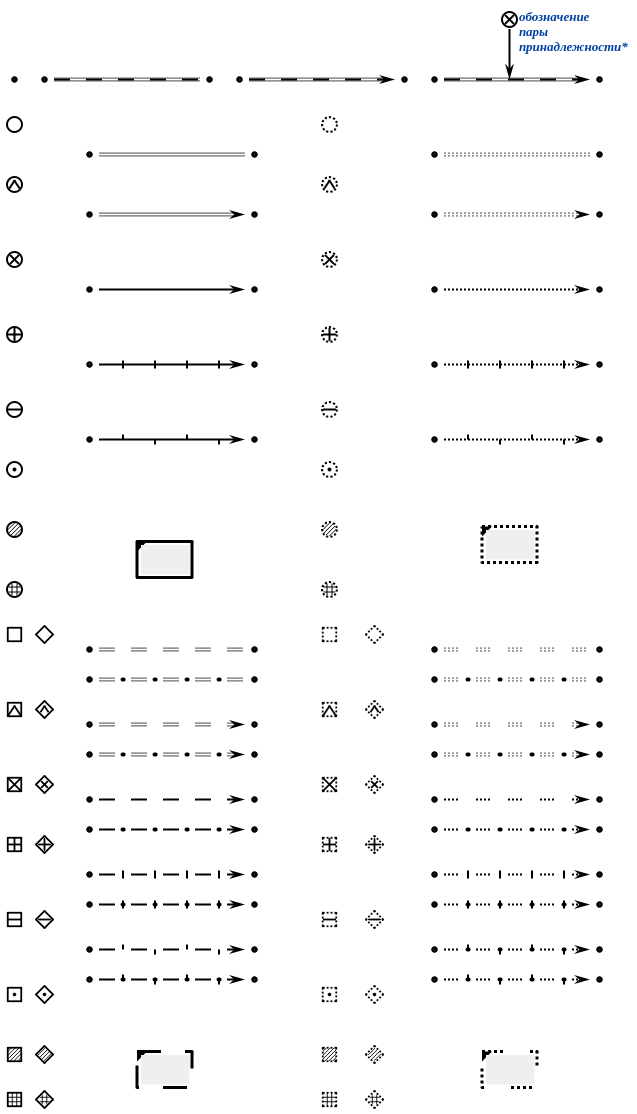
\includegraphics[scale=0.8]{images/intro/scg/SCg-full.png}
\end{figure}

\bigskip
Трудно сразу поверить, что на основе такого простого алфавита можно построить удобный и \uline{универсальный} \textit{графовый язык}. В рамках \textit{Документации Технологии OSTIS} мы постараемся Вас в этом убедить. Кроме того, нас не должна настораживать простота алфавита, поскольку человечество имеет большой опыт кодирования, хранения в памяти и передачи по каналам связи самых различных информационных ресурсов, используя алфавит, состоящий только из двух классов элементов --- единиц и нулей. 

Мы ведем речь о принципиально ином (графовом) способе кодирования информации в \textit{компьютерных системах}, но стараемся при этом свести это кодирование к достаточно простому алфавиту хотя бы для того, чтобы искусственно не усложнять проблему создания нового поколения компьютеров, основанных на указанном способе кодирования информации. 

Расширения \textit{Ядра SCg-кода} рассмотрим как направления перехода от текстов \textit{Ядра SCg-кода} к более компактным текстам. Но, поскольку это приводит к усложнению \textit{Синтаксиса SCg-кода} и, в первую очередь, к расширению \textit{Алфавита SCg-кода\scnsupergroupsign}, делать такие расширения необходимо обоснованно с учетом частоты встречаемости в рамках \textit{баз знаний ostis-систем} соответствующих фрагментов.

\subsection{Денотационная семантика SCg-кода}
\label{sec_scg_semantics}

В \textit{SCg-коде} выделяются Ядро SCg-кода и его расширения. 
\textbf{\textit{Алфавит Ядра SCg-кода\scnsupergroupsign}} --- алфавит \textit{sc.g-элементов}, графически изображаемых \textit{sc-элементы}. \textit{Алфавит Ядра SCg-кода\scnsupergroupsign} взаимно однозначно соответствует \textit{Алфавиту SC-кода\scnsupergroupsign}.

\textit{Денотационная семантика Ядра SCg-кода} соответствует \textit{Денотационной семантике SC-кода}. Это продемонстрировано на рисунке.

\textbf{\textit{Таблица. Алфавит Ядра SCg-кода\scnsupergroupsign}}
\begin{figure}[h]
	\centering
	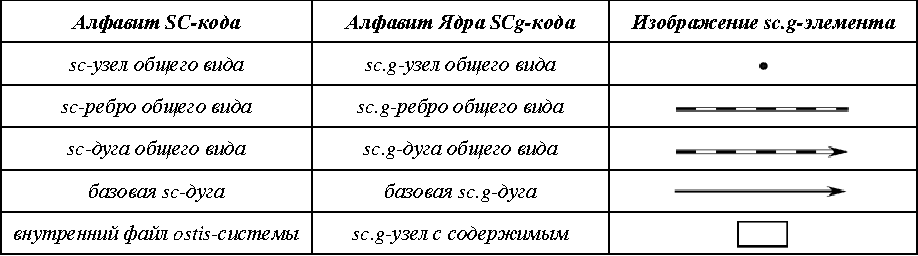
\includegraphics[scale=0.8]{images/intro/scg/SCg-core-alphabet.pdf}
\end{figure}

\textit{Алфавит Ядра SCg-кода\scnsupergroupsign} представлен следующими элементами:
\begin{textitemize}
	\item \textbf{\textit{sc.g-узел общего вида}} --- \textit{sc.g-элемент}, являющийся графическим изображением \textit{sc-узла общего вида}. Все \textit{sc-узлы}, не являющиеся знаками файлов, в тексте (конструкции) \textit{Ядра SCg-кода}, изображаются в виде небольших чёрных кругов одинакового диаметра, который обозначим через $\bm{d}$, и точная величина которого зависит от масштаба отображения \textit{sc.g-текста};
	
	\item \textbf{\textit{sc.g-ребро общего вида}} --- \textit{sc.g-элемент}, являющийся графическим изображением \textit{sc-ребра общего вида}. Каждое \textit{sc-ребро} в \textit{Ядре SCg-кода} изображается в виде широкой линии, в которой чередуются фрагменты со сплошной заливкой и без заливки, не имеющей самопересечений и имеющей общую толщину, равную примерно $\bm{0.7d}$;
	
	\item \textbf{\textit{sc.g-дуга общего вида}} --- \textit{sc.g-элемент}, являющийся графическим изображением \textit{sc-дуги общего вида}. Каждая \textit{sc-дуга} в \textit{Ядре SCg-кода} изображается в виде широкой линии, в которой чередуются фрагменты со сплошной заливкой и без заливки, не имеющей самопересечений, имеющей общую толщину, равную примерно $\bm{0.7d}$ и имеющей изображение стрелочки на одном из концов этой линии;
	
	\item \textbf{\textit{базовая sc.g-дуга}} --- \textit{sc.g-элемент}, являющийся графическим изображением \textit{базовой sc-дуги}. Каждая входящая в состав sc-текста \textit{базовая sc-дуга} в \textit{Ядре SCg--кода} изображается в виде линии произвольной формы, не имеющий самопересечений, имеющий толщину $\bm{0.4d}$, и имеющей изображение стрелочки на одном из ее концов;
	
	\item \textbf{\textit{внутренний файл ostis-системы}} --- \textit{sc-узел}, являющийся знаком \textit{внутреннего файла ostis-системы}, sc-знак \textit{внутреннего файла ostis-системы};
	
	\item \textbf{\textit{sc.g-узел с содержимым}} --- \textit{sc.g-узел}, имеющий содержимое, sc.g-узел, являющийся знаком внутреннего файла ostis-системы, sc.g-рамка. \textit{sc.g-рамка} --- это всегда прямоугольник, максимальный размер которого не ограничивается, но минимальный фиксируется и соответствует \textit{sc.g-рамке}, внутри которой обозначаемый ею \textit{файл} не отображается. Каждый входящий в sc-текст \textit{sc-узел, имеющий содержимое}, в \textit{Ядре SCg-кода} изображается в виде прямоугольника произвольного размера с толщиной линии $\bm{0.6d}$. Внутри этого прямоугольника отображается \textit{файл}, обозначаемый изображаемым \textit{sc-узлом}. Если нет необходимости изображать в тексте сам \textit{файл}, то \textit{sc-узел}, обозначающий такой \textit{файл}, в \textit{sc.g-тексте} изображается в виде прямоугольника со сторонами $\bm{2d}$ по вертикали и $\bm{4d}$ по горизонтали.
\end{textitemize}

\subsection{Иерархическое семейство подъязыков, семантически эквивалентных SCg-коду}
\label{sec_scg_extensions}

\begin{SCn}
\begin{scnrelfromlist}{ключевой знак}
	\scnitem{Первое направление расширения Ядра SCg-кода}
	\scnitem{Второе направление расширения Ядра SCg-кода}
	\scnitem{Третье направление расширения Ядра SCg-кода}
	\scnitem{Четвертое направление расширения Ядра SCg-кода}
	\scnitem{Пятое направление расширения Ядра SCg-кода}
	\scnitem{Шестое направление расширения Ядра SCg-кода}
	\scnitem{Седьмое направление расширения Ядра SCg-кода}
\end{scnrelfromlist}
\end{SCn}

\textbf{\textit{Первое направление расширения Ядра SCg-кода}}

\textit{Первое направление синтаксического расширения Ядра SCg-кода} --- это \uline{приписывание} некоторым \mbox{sc.g-элементам} \textit{основных sc-идентификаторов*} (чаще всего --- строковых идентификаторов, то есть имен) \textit{sc-элементов} , изображаемых этими \textit{sc.g-элементами}. Указываемые идентификаторы являются уникальным для каждого идентифицируемого (именуемого) \textit{sc.g-элемента}. Приписывание \textit{sc.g-элементам} уникальных идентификаторов дает возможность в рамках одного \textit{sc.g-текста} дублировать (копировать) некоторые \textit{sc.g-узлы} при условии, если \uline{всем} таким копиям будут приписаны соответствующие идентификаторы. Такое дублирование \textit{sc.g-узлов} является дополнительным средствам \uline{наглядного} размещения \textit{sc.g-текстов}. Кроме того, приписывание \textit{sc.g-элементу} соответствующего ему основного (уникального) \textit{sc-идентификатора*} представляет собой более компактный вариант изображения \textit{sc.g-текстов}.

\textbf{\textit{Пример sc.g-текста, трансформируемого по Первому направлению расширения Ядра SCg-кода}}

\begin{figure}[h]
	\centering
	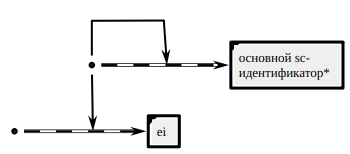
\includegraphics[scale=0.8]{images/intro/scg/scg_transf1.png}
\end{figure}

Здесь (в левом нижнем углу приведенного sc.g-текста) представлен \textit{sc.g-узел общего вида}, изображающий \textit{sc-узел общего вида}, которому соответствует \textit{основной sc-идентификатор*} в виде строки ``\textbf{\textit{ei}}''.

\bigskip
Трансформация \textit{sc.g-текста} по \textit{Первому направлению расширения Ядра SCg-кода}:
\begin{figure}[h]
	\centering
	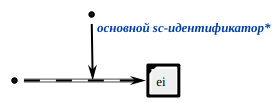
\includegraphics[scale=0.8]{images/intro/scg/scg_transf2.png}
\end{figure}
\textit{sc.g-узлу общего вида} изображающему \textit{sc-узел}, внешним идентификатором которого является строка ``\textit{основной sc-идентификатор*}'' и который, соответственно является знаком \textit{бинарного ориентированного отношения}, каждая \textit{пара} которого связывает идентифицируемый \textit{sc-элемент} с его основным внешним sc-идентификатором, приписывается указанный внешний идентификатор изображаемого им \textit{sc-элемента}.

\bigskip
Трансформация \textit{sc.g-текста} по \textit{Первому направлению расширения Ядра SCg-кода}:
\begin{figure}[h]
	\centering
	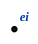
\includegraphics[scale=0.8]{images/intro/scg/scg_transf3.png}
\end{figure}

В результате данной трансформации исходный \mbox{\textit{sc.g-текст}} трансформируется в один \textit{sc.g-общего вида}, которому приписывается \textit{основной sc-идентификатор} ``\textit{\textbf{ei}}''.

Подчеркнем, что рассматриваемая трансформация преобразует исходный текст Ядра \textit{SCg-кода} в текст, семантически эквивалентный, но принадлежащий не Ядру \textit{SCg-кода}, а его расширению.

\textbf{\textit{Второе направление расширения Ядра SCg-кода}}

\textit{Второе направление расширения Ядра SCg-кода} --- это уточнение типологии \textit{константных постоянных сущностей} и расширение \textit{Алфавита Ядра SCg-кода\scnsupergroupsign}, позволяющее типологию \textit{константных постоянных сущностей} привести в соответствие с синтаксической типологией новых вводимых элементов \textit{Алфавита SCg-кода\scnsupergroupsign}. Рассмотрим подробнее sc.g-элементы, знаки \textit{константных постоянных сущностей} различного вида. Графическим признаком \textit{константных постоянных sc-узлов} в конструкциях SCg-кода является их изображение в виде \uline{окружностей} диаметра $3d$, где $d$ --- диаметр sc.g-узла общего вида. Такое изображение является более компактной записью факта принадлежности заданного sc-узла (назовем его $\bm{vi}$) классу sc-констант и классу обозначений постоянных сущностей. Запись этого факта в \textit{Ядре SCg-кода} потребует (1) явного изображения sc-узла, обозначающего класс всевозможных константных sc-элементов (класс \textit{sc-констант}), (2) явного изображения базовой sc-дуги, соединяющего изображение sc-узла, обозначающего класс sc-констант, с изображением заданного константного sc-узла, (3) явного изображение sc-узла, обозначающего класс всевозможных sc-элементов, обозначающих \textit{постоянные сущности}, (4) явного изображения базовой sc-дуги, соединяющего изображение sc-узла, обозначающего класс обозначений \textit{постоянных сущностей} с изображением рассматриваемого sc-узла $\bm{vi}$ (см. \textit{Файл. Изображение спецификации sc.g-элемента средствами Ядра SCg-кода и Первого расширения Ядра SCg-кода}).

\textit{Второе направление расширения Ядра SCg-кода} --- это уточнение типологии \textit{константных постоянных сущностей} и расширение \textit{Алфавита Ядра SCg-кода\scnsupergroupsign}, позволяющее типологию \textit{константных постоянных сущностей} привести в соответствие с синтаксической типологией новых вводимых элементов \textit{Алфавита SCg-кода\scnsupergroupsign}. Рассмотрим подробнее sc.g-элементы, знаки \textit{константных постоянных сущностей} различного вида. Графическим признаком \textit{константных постоянных sc-узлов} в конструкциях SCg-кода является их изображение в виде \uline{окружностей} диаметра $3d$, где $d$ --- диаметр sc.g-узла общего вида. Такое изображение является более компактной записью факта принадлежности заданного sc-узла (назовем его $\bm{vi}$) классу sc-констант и классу обозначений постоянных сущностей. Запись этого факта в \textit{Ядре SCg-кода} потребует:
\begin{textitemize}
	\item явного изображения sc-узла, обозначающего класс всевозможных константных sc-элементов (класс \textit{sc-констант});  
	\item явного изображения базовой sc-дуги, соединяющего изображение sc-узла, обозначающего класс sc-констант, с изображением заданного константного sc-узла; 
	\item явного изображение sc-узла, обозначающего класс всевозможных sc-элементов, обозначающих \textit{постоянные сущности};
	\item явного изображения базовой sc-дуги, соединяющего изображение sc-узла, обозначающего класс обозначений \textit{постоянных сущностей} с изображением рассматриваемого sc-узла $\bm{vi}$ (см. \textit{Файл. Изображение спецификации sc.g-элемента средствами \textit{Ядра SCg-кода} и \textit{Первого расширения Ядра SCg-кода}}).
\end{textitemize}

\bigskip
Общепринятая запись данного факта выглядит следующим образом:

``\textit{sc-константа} $\ni \bm{vi}$; \textit{постоянная сущность} $\ni \bm{v_i};$''
\bigskip

\begin{textitemize}
	\item \textit{Константные постоянные sc-ребра} в конструкциях SCg-кода изображаются в виде двойной линии, каждая из которых имеет толщину примерно $d/7$, а расстояние между ними равно примерно $3d/7$. 
	\item \textit{Константные постоянные sc-дуги} изображаются в виде такой же двойной линии, но со стрелочкой. Все \textit{базовые sc-дуги}, а также все sc-узлы, имеющие содержимое, по определению являются \textit{константными постоянными sc-элементами}. 
	\item \textit{Константные sc.g-узлы}, изображаемые окружностями диаметра $3d$ и толщиной границы $d/5$, обозначают \textit{константные постоянные сущности}, о которых мало что известно, но известно то, что они не являются парами (то есть множествами, \textit{мощность*} которых равна 2) и, следовательно, не могут быть изображёны в виде sc.g-дуг или sc.g-рёбер. Но, если при этом об обозначаемой \textit{константной постоянной сущности} ($\bm{vi}$) известно, что она является классом сущностей, то явное указание принадлежности sc-элемента \textit{vi} всевозможных классов можно заменить на специальное графическое изображение sc-элемента \textit{vi}, предполагаемое указанную принадлежность. Это приводит к расширению  \textit{Алфавита SCg-кода\scnsupergroupsign} (см. \textit{Примеры sc.g-текстов, трансформируемых по Второму направлению расширения Ядра SCg-код}).
\end{textitemize}


Аналогичным образом (см. \textit{Примеры sc.g-текстов, трансформируемых по Второму направлению расширения Ядра SCg-код}) вводятся: 
\begin{textitemize}
	\item \textit{sc.g-узел}, являющийся изображением \textit{класса};  
	\item \textit{sc.g-узел}, являющийся изображением \textit{класса классов};  
	\item \textit{sc.g-узел}, являющийся изображением \textit{отношения}; 
	\item \textit{sc.g-узел}, являющийся изображением \textit{ролевого отношения}; 
	\item \textit{sc.g-узел}, являющийся изображением \textit{структуры};  
	\item \textit{sc.g-узел}, являющийся изображением \textit{небинарной связки};
	\item \textit{sc.g-узел}, являющийся изображением \textit{первичной сущности} (терминальной сущности, которая не является множеством, а также файлом, хранимым в памяти ostis-системы).
\end{textitemize}

Важное место среди константных постоянных сущностей занимают \textit{константные постоянные пары принадлежности}, обозначаемое соответствующими \textit{sc.g-дугами}. Такие пары принадлежности и обозначающие их sc.g-дуги бывают позитивными, негативными и нечеткими. Константная постоянная позитивная sc.g-дуга принадлежности есть ничто иное, как \textit{базовая sc.g-дуга}. Константная постоянная негативная sc.g-дуга принадлежности изображается в виде \textit{базовой sc.g-дуги}, перечеркнутой штриховыми черточками. Константная постоянная нечёткая sc.g-дуга принадлежности изображается в виде "недочеркнутой"{} \textit{базовой sc.g-дуги}, с каждой стороны которой отображаются штрихи, по длине равные половине от длины штрихов, которыми перечеркнута \textit{константная постоянная негативная sc.g-дуга}.

\textbf{\textit{Третье направление расширения Ядра SCg-кода}}

\textit{Третье направление расширения Ядра SCg-кода} --- это расширение его алфавита путем введения дополнительных sc.g-элементов, обозначающих \textit{константные временные сущности} различного вида. Признаком sc.g-элементов, обозначающих \textit{константные временные сущности} являются точечные линии (линии, состоящие из точек, размер которых равен размеру изображаемой линии и которые близко расположены друг к другу на расстоянии, равном половине их размера), с помощью которых рисуются окружности при изображении sc-узлов, а также линии при изображении sc-коннекторов.

Результатом \textit{Третьего направления расширения Ядра SCg-кода} является введение следующих видов \textit{sc.g-элементов} (см. \textit{Примеры sc.g-текстов, трансформируемых по Третьему направлению расширения Ядра SCg-кода}).

\textbf{\textit{Четвёртое направление расширения Ядра SCg-кода}}

\textit{Четвёртое направление расширения Ядра SCg-кода} --- это расширение его алфавита путем введения дополнительных элементов, обозначающих \textit{переменные постоянные сущности} различного вида. Признаком sc.g-элементов, обозначающих сущности указанного класса, являются квадратики для изображения обозначений \textit{переменных постоянных сущностей}, не являющихся бинарными связями, а также пунктирные и штрих-пунктирные линии для изображения \textit{переменных постоянных бинарных связей}. 

Подчеркнем, что \textit{переменные постоянные сущности} могут отличаться друг от друга по характеру их \textit{области значений*}. Этими значениями в общем случае могут быть как \textit{константные постоянные сущности}, так и \textit{переменные постоянные сущности}. В любом случае, значение \textit{переменной сущности} является либо \textit{константной сущностью}, либо \textit{переменной сущностью}. Если каждое значение переменной является константой, то такую переменную будем называть \textit{переменной первого уровня}. Если каждое значение переменной является \textit{переменной первого уровня}, то такую переменную будем называть \textit{переменной второго уровня}. 

\textbf{\textit{переменная постоянная сущность первого уровня}} (первичная sc-переменная), не являющаяся бинарной связью --- это переменная, каждым значением которой является \textit{константная постоянная сущность}, не являющаяся бинарной связью. Такая переменная изображается квадратиком, который ориентирован по вертикали и горизонтали. 

\textit{переменная постоянная сущность второго уровня} (вторичная sc-переменная), не являющаяся бинарной связью, изображается квадратиком, повернутым на 45$^\circ$. 

Указанная выше семантика таких изображений приписывается \uline{по умолчанию}. Это означает, что, если обозначаемая sc-переменная имеет более сложную структуру области её значений (является sc-переменной третьего и выше уровня или sc-переменной, значения которой имеют различный логический уровень), то эта область должна быть специфицирована явно, при этом такая sc-переменная в SCg-коде изображается так же, как первичная sc-переменная.

\textbf{\textit{Пятое направление расширения Ядра SCg-кода}}
	
\textit{Пятое направление расширения Ядра SCg-кода} --- это расширение его алфавита путем введения дополнительных \textit{sc.g-элементов}, обозначающих \textit{переменные временные сущности} различного вида. Указанные дополнительные \textit{sc.g-элементы} аналогичны тем, которые введены в рамках \textit{Четвертого направления расширения Ядра SCg-кода}, и отличаются только тем, что в \textit{Пятом направлении расширении Ядра SCg-кода} речь идёт о переменных \uline{временных} сущностях, а в \textit{Четвертом направлении расширения Ядра SCg-кода} --- о переменных \uline{постоянных} сущностях.

\textbf{\textit{Шестое направление расширения Ядра SCg-кода}}

\textit{Шестое направление расширения Ядра SCg-кода} --- это введение в SCg-код \textit{sc.g-контуров} и \textit{sc.g-шин} как средств структуризации sc.g-текстов и повышения наглядности при их размещении. Подчеркнем, что и sc.g-контуры, и sc.g-шины, и sc.g-рамки являются специальными видами sc.g-элементов. При этом sc.g-контуры и sc.g-рамки являются sc.g-ограничителями (ограничителями SCg-кода).

Каждый \textbf{\textit{sc.g-контур}} изображается (в 2D-модификации) в виде замкнутой ломаной линии со скругленными изломами, ограничивающей некоторый фрагмент sc.g-текста и обозначает множество всех \uline{sc-элементов}, sc.g-изображения которых оказались внутри этого контура. Толщина указанной линии составляет примерно $\bm{0.4d}$, где \textbf{\textit{d}} --- диаметр \textit{sc.g-узла общего вида}.

Обозначение \textit{множества sc-элементов}, изображаемое \textit{sc.g-контуром}, может быть как константным, так и переменным. Соответственно этому линия, изображающая \textit{sc.g-контур} может быть: 

\begin{textitemize}
	\item сплошной непунктирной линией,
	\item точечной непунктирной линией,
	\item сплошной пунктирной линией,
	\item точечной пунктирной линией.
\end{textitemize}

\bigskip
Семантическим эквивалентом \textit{sc.g-контуру} является \textit{sc.g-узел, обозначающий структуру}. Использование \textit{sc.g-контура} вместо указанного \textit{sc.g-узла} исключает необходимость явно изображать \textit{sc-дуги принадлежности}, выходящие из этого \textit{sc.g-узла}. Это существенно повышает уровень наглядности \textit{sc.g-текста}.

Если представленный внутри \textit{sc.g-контура} текст не является \textit{sc.g-текстом}, то считается, что на самом деле внутренностью \textit{sc.g-контура} является \textit{sc.g-текст}, являющийся результатом перевода предоставленного текста в \textit{SCg-код}.

Каждая \textbf{\textit{sc.g-шина}} представляет собой замкнутую или незамкнутую линию толщиной примерно равной диаметру \textit{sc.g-узла общего вида}, которая инцидентна только одному \textit{sc.g-элементу} и семантически ему эквивалентна. Идея введения \textit{sc.g-шин} заключается в увеличении «размеров» \textit{sc.g-элементов} для расширения их области инцидентности. Особенно актуально это для \textit{sc.g-узлов}, имеющих большое число инцидентных им \textit{sc.g-коннекторов}.

\bigskip
\textbf{\textit{Седьмое направление расширения Ядра SCg-кода}}
	
\textit{Седьмое направление синтаксического расширения Ядра SCg-кода} --- это переход от 2D-изображений \textit{sc.g-текстов} к 3D-изображениям.

Одним из вариантов трехмерного изображения \textit{sc.g-текстов} является следующий:
\begin{textitemize}
	\item все sc.g-узлы изображаются, как и ранее, \uline{плоскими} графическими примитивами. При изменении точки просмотра они \uline{всегда} "поворачиваются"{} параллельно плоскости экрана, но их масштаб (размер на экране) при удалении от точки просмотра \uline{уменьшается};
	\item аналогичным "плоским"\ образом изображаются \textit{sc.g-рамки} с их "внутренним"\ содержанием, а также внешние идентификаторы, приписываемые \textit{sc.g-элементам};
	\item \textit{sc.g-коннекторы} изображаются \uline{непересекающимися} линиями в трехмерном пространстве (заметим, что при изображении \textit{sc.g-текстов} на плоскости пересечение \textit{sc.g-коннекторов} часто снижает наглядность, "читабельность"{} \textit{sc.g-текстов}). Т.е. \textit{sc.g-коннекторы}, которые на плоскости изображаются двойными линиями, в пространстве  цилиндрическими, "трубчатыми линиями"{} с находящейся внутри тонкой, но просвечивающейся осевой линией;
	\item \textit{sc.g-контур} в пространстве визуализируется несколькими (!) специального вида точками --- например там, где есть точки инцидентности \textit{sc.g-контура} с \uline{внешними} \textit{sc.g-коннекторами}. При этом \textit{sc.g-контур} становится виден только по команде просмотра указываемого контура (указание контура --- это указание одной из его точек инцидентности). По этой команде цветом выделяются все граничные точки контура (точки инцидентности) и все внутренние \textit{sc.g-элементы} контура. Если просматривается  несколько контуров, то используется несколько цветов.
\end{textitemize}

Вторым вариантом 3D-визуализации \textit{sc.g-текстов} является размещение \textit{sc.g-текстов} на параллельных плоскостях (слоях) с “прошивками”\ между этими слоями, соединяющими синонимичные \textit{sc.g-узлы}, то есть \textit{sc.g-узлы}, имеющие одинаковые приписываемые им внешние идентификаторы. Такой вариант плоской, но многослойной визуализации \textit{sc.g-текстов} дает возможность широко использовать те средства просмотра и редактирования \textit{sc.g-текстов}, которые разработаны для плоской их визуализации.

\section{Язык внешнего линейного представления конструкций SC-кода --- SCs-код (Semantic Code string)}
\label{sec_scs}

\begin{SCn}
\begin{scnrelfromlist}{подраздел}
	\scnitem{\ref{sec_scs_syntax}~\nameref{sec_scs_syntax}}
	\scnitem{\ref{sec_scs_semantics}~\nameref{sec_scs_semantics}}
	\scnitem{\ref{sec_scs_extensions}~\nameref{sec_scs_extensions}}
\end{scnrelfromlist}

\begin{scnrelfromlist}{ключевое понятие}
	\scnitem{sc.s-предложение}
	\scnitem{sc.s-ограничитель}
	\scnitem{sc.s-разделитель}
	\scnitem{sc.s-модификатор}
	\scnitem{sc.s-элемент}
	\scnitem{sc.s-коннектор}
	\scnitem{sc.s-ребро}
	\scnitem{sc.s-дуга}
\end{scnrelfromlist}

\begin{scnrelfromlist}{ключевой знак}
	\scnitem{SCs-код}
	\scnitem{Алфавит SCs-кода\scnsupergroupsign}
	\scnitem{Синтаксис SCs-кода}
	\scnitem{Денотационная семантика SCs-кода}
	\scnitem{Иерархическое семейство подъязыков, семантически эквивалентных SCs-коду}
\end{scnrelfromlist}
\end{SCn}

\begin{SCn}
\scnheader{SCs-код}
\scnidtf{Semantic Code string}
\scnidtf{Язык линейного представления знаний ostis-систем}
\scnidtf{Множество всевозможных текстов \textit{SCs-кода}}
\scnidtf{Язык внешнего линейного представления конструкций внутреннего языка ostis-систем}
\end{SCn}

\textbf{\textit{SCs-код}} представляет собой множество линейных текстов (\textit{sc.s-текстов}), каждый из которых состоит из предложений (\textit{sc.s-предложений}), разделенных друг от друга двойной \textit{точкой с запятой} (разделителем \textit{sc.s-предложений}). При этом \mbox{\textit{sc.s-предложение}} представляет собой последовательность \textit{sc-идентификаторов}, являющихся именами описываемых \textit{сущностей} и разделяемых между собой различными \textit{sc.s-разделителями} и \textit{sc.s-ограничителями}.

\subsection{Синтаксис SCs-кода}
\label{sec_scs_syntax}

\begin{SCn}
	\scnheader{Алфавит SCs-кода\scnsupergroupsign}
	\scnidtf{Алфавит символов SCs-кода\scnsupergroupsign}
	\scnidtf{множество символов SCs-кода}
	\scnidtf{символ, используемый в текстах SCs-кода}
	\scnidtf{Язык внешнего линейного представления информационных конструкций
		внутреннего языка ostis-систем}
	\begin{scnreltoset}{объединение}
		\scnitem{Алфавит символов, используемых в sc.s-разделителях\scnsupergroupsign}
		\scnitem{Алфавит символов, используемых в sc.s-ограничителях\scnsupergroupsign}
		\scnitem{Алфавит символов, используемых в sc-идентификаторах\scnsupergroupsign}
			\begin{scnreltoset}{объединение}
				\scnitem{Алфавит символов, используемых в простых строковых sc-идентификаторах\scnsupergroupsign}
				\scnitem{Алфавит символов, используемых в sc-выражениях\scnsupergroupsign}			
			\end{scnreltoset}
		\scnitem{Алфавит символов, используемых в неоднозначных sc.s-изображениях sc-узлов\scnsupergroupsign}
	\end{scnreltoset}
\end{SCn} 

\textbf{\textit{Алфавит SCs-кода\scnsupergroupsign}} строится на основе современных общепринятых наборов символов, что позволяет упростить разработку средств для работы с \textit{sc.s-текстами} с использованием современных технологий.

В состав \textit{sc.s-текстов}, как и в состав текстов любых других языков, являющихся вариантами внешнего отображения текстов \textit{SC-кода}, могут входить различные файлы, в том числе естественно-языковые или даже файлы, содержащие другие \textit{sc.s-тексты}. В общем случае в таких файлах могут использоваться самые разные символы, в связи с чем будем считать, что в \textit{Алфавит SCs-кода\scnsupergroupsign} эти символы не включаются.

\textbf{Алфавит символов, используемых в \textit{sc.s-разделителях}\scnsupergroupsign} состоит из: пробел, точка с запятой, двоеточие, круглый маркер и знак равенства.

\textbf{Алфавит символов, используемых в \textit{sc.s-разделителях}\scnsupergroupsign}, изображающих связь инцидентности sc-элементов состоит из: `` < ''{}, `` > ''{}, `` | ''{}, `` - ''{}.



\textbf{Алфавит символов, используемых в \textit{sc.s-разделителях}} состоит из: пробел, точка с запятой, двоеточие, круглый маркер и знак равенства.

\textbf{Алфавит символов, используемых в \textit{sc.s-разделителях}}, изображающих связь инцидентности sc-элементов состоит из: `` < ''{}, `` > ''{}, `` | ''{}, `` --- ''{}.

\textbf{Базовый алфавит символов, используемых в \textit{sc.s-коннекторах}} состоит из: `` $\sim$ ''{}, знак подчеркивания, знак равенства, двоеточие, `` < ''{}, `` > ''{}, `` --- ''{}, `` | ''{}, `` / ''{}.
	
\textbf{Расширенный алфавит символов, используемых в \textit{sc.s-коннекторах}\scnsupergroupsign} состоит из:
	``$\in$''{}, 
	``$\ni$''{}, ``$\subseteq$''{}, ``$\supseteq$''{},   ``$\subset$''{}, ``$\supset$''{}, ``$\leq$''{},  ``$\geq$''{}, ``$\Leftarrow$''{}, ``$\Rightarrow$''{}, ``$\leftarrow$''{}, ``$\rightarrow$''{}, 
	``$\Leftrightarrow$''{}.


При необходимости комбинации указанных признаков перечисленные символы комбинируются так, как показано в параграфе "\textit{Описание sc.s-разделителей и sc.s-ограничителей}"{}.

Как в \textit{Базовом}, так и в \textit{Расширенном Алфавитах} \textit{sc.s-коннекторов} используются следующие общие признаки, характеризующие тип изображаемого \textit{sc-коннектора}:
\begin{textitemize}
	\item знак подчеркивания как признак изображений переменных \textit{sc-коннекторов} (один знак подчеркивания для \textit{sc-коннекторов}, являющихся первичными \textit{sc-переменными}, два знака подчеркивания для \textit{sc-коннекторов}, являющихся вторичными \textit{sc-переменными (sc-метапеременными)});
	\item вертикальная черта `` $ | $ ''{} как признак изображений \textit{негативных sc-дуг принадлежности}; 
	\item косая черта `` $ / $ ''{} как признак изображений \textit{нечетких sc-дуг принадлежности};
	\item тильда `` $ \sim $ ''{} как признак изображений \textit{временных sc-дуг принадлежности}.   
\end{textitemize}

Для упрощения процесса разработки исходных текстов \textit{баз знаний} с использованием \textit{SCs-кода} и создания соответствующих средств вводятся два алфавита символов. \textit{Базовый алфавит символов, используемых в sc.s-коннекторах\scnsupergroupsign} включает только символы, входящие в переносимый набор символов и имеющиеся на стандартной современной клавиатуре. Таким образом, для разработки исходных текстов баз знаний, использующих только \textit{Базовый алфавит символов, используемых в sc.s-коннекторах\scnsupergroupsign} достаточно обычного текстового редактора. \textit{Расширенный алфавит символов, используемых в sc.s-коннекторах\scnsupergroupsign} включает также дополнительные символы, которые позволяют сделать sc.s-тексты (и sc.n-тексты) более читабельными и наглядными. Для визуализации и разработки sc.s-текстов с использованием расширенного алфавита требуется наличие специализированных средств.

\textbf{Алфавит символов, используемых в \textit{sc.s-ограничителях}\scnsupergroupsign} состоит из: ``( ''{}, ``)''{}, ``*''{}.

\textbf{Алфавит символов, используемых в неоднозначных \textit{sc.s-изображениях sc-узлов}\scnsupergroupsign} состоит из:
``\{''{}, ``\}''{}, 
``-''{}, ``!''{}, ``~[ \,''{}, ``~] \,{}.

\bigskip
\textbf{\textit{Описание sc.s-разделителей и sc.s-ограничителей}}

\textbf{\textit{sc.s-разделитель}} и \textbf{\textit{sc.s-ограничитель}} являются важными элементами \textit{SCs-кода}.

Существует \textit{sc.s-разделитель}, используемый для структуризации \textit{sc.s-предложений} и \textit{sc.s-разделитель} \textit{sc.s-предложений}.

\textit{sc.s-разделить} --- разделитель, используемый в \textit{sc.s-текстах}. \textit{sc.s-разделитель} разбивается на:
\begin{textitemize}
	\item \textit{sc.s-разделитель}, используемый для структуризации \textit{\textit{sc.s-предложений}}.
	\begin{textitemize}
		\item Разделяет \textit{sc-идентификатор бинарного отношения} и второй компонент одной из связок этого отношения в случае, если указанное бинарное отношение и его связка связаны \textit{константной sc-дугой принадлежности}. Представляется в виде двоеточия.
		\item Разделяет \textit{sc-идентификатор бинарного отношения} и второй компонент одной из связок этого отношения в случае, если указанное бинарное отношение и его связка связаны \textit{переменной sc-дугой принадлежности}. Представляется в виде двойного двоеточия.
	\end{textitemize}
	\item \textit{sc.s-разделитель \textit{sc.s-предложений}}, представляется в виде двойной точки с запятой.    
\end{textitemize}

\bigskip
\textbf{\textit{sc.s-ограничитель}} представляется в виде: $(![  (\ast ]! \cup ![  \ast) ]!)$

Круглые скобки со звездочкой ограничивают присоединенные \textit{sc.s-предложения}, которые, в свою очередь, могут иметь в своем составе другие присоединенные \textit{sc.s-предложения}.

Также существует \textbf{\textit{sc.s-коннектор}}. Типология \textit{sc.s-коннекторов} полностью соответствует типологии \textit{sc.g-коннекторов}, и, тем более, \textit{sc-коннекторов}, т.к. она учитывает устоявшиеся традиции изображения связок целого ряда конкретных отношений.

\begin{SCn}
\scnheader{sc.s-коннектор}
\scnidtf{изображение \textit{sc-коннектора} во внешнем тексте SCs-кода или SCn-кода}
\scnsubset{sc.s-разделитель}
\end{SCn}

Выделяют следующие \textit{sc.s-коннекторы}:
\begin{textitemize}
	\item \textit{ориентированный \textit{sc.s-коннектор}},
	\item \textit{неориентированный \textit{sc.s-коннектор}};
	\item \textit{\textit{sc.s-коннектор}}, соответствующий \textit{sc.g-дуге принадлежности},
	\item \textit{\textit{sc.s-коннектор}}, соответствующий \textit{sc.g-коннектору}, который не является \textit{sc.g-дугой}.
\end{textitemize}

Типология \textit{sc.s-коннекторов} полностью соответствует типологии \textit{sc.g-коннекторов}, и, тем более, \textit{sc-коннекторов}, так как она учитывает устоявшиеся традиции изображения связок целого ряда конкретных отношений.

На множестве \textit{sc-элементов} задано бинарное ориентированное отношение инцидентности sc-элементов, а так же подмножество этого отношения --- отношение инцидентности входящих \textit{sc-дуг}, каждая пара которого связывает sc-дугу с тем sc-элементом, в который она входит. В \textit{SC-коде} \textit{sc-коннекторы} могут соединять между собой не только \textit{sc-узел} с \textit{sc-узлами}, но и \textit{sc-узел} с \textit{sc-коннектором} и даже \textit{sc-коннектор} с \textit{sc-коннектором}. В последнем случае, указывая инцидентность sc-коннекторов, необходимо уточнить, какой из них является соединяемым (связываемым), а какой-соединяющим (связующим). Поэтому отношение инцидентности, заданное на множестве sc-элементов является ориентированным. Первый компонент пары этого отношения – связующий \textit{sc-коннектор}, а второй --- связуемый \textit{sc-элемент}. Очевидно, что связующий \textit{sc-элемент} всегда является \textit{sc-коннектором}, а \textit{sc-узел} может быть только связуемым.

\textit{sc.s-разделитель}, изображающий связь инцидентности \textit{sc-элементов} разбивается на:
\begin{textitemize}
	\item знак инцидентности “правого” \textit{sc-коннектора} --- знак инцидентности \textit{sc-коннектора}, \textit{sc-идентификатор} которого находится справа, изображается в виде `` $ \vdash$ ''{};
	\item знак инцидентности “левого” \textit{sc-коннектора} --- знак инцидентности \textit{sc-коннектора}, \textit{sc-идентификатор} которого находится слева, изображается в виде `` $ \dashv$ ''{};
	\item знак инцидентности входящей \textit{sc-дуги} справа --- знак инцидентности \textit{sc-дуги}, \textit{sc-идентификатор} который находится справа, изображается в виде `` $ |<$ ''{};
	\item знак инцидентности входящей \textit{sc-дуги} слева --- знак инцидентности \textit{sc-дуги}, \textit{sc-идентификатор} который находится слева, изображается в виде `` $ >| $ ''{}.
\end{textitemize}

\begin{SCn}
\scnheader{sc.s-разделитель, изображающий связь инцидентности sc-элементов}
\begin{scnrelfromset}{разбиение}
	\scnitem{знак инцидентности “правого” sc-коннектора}
	\begin{scnindent}
		\scnidtf{знак инцидентности sc-коннектора, sc-идентификатор которого находится справа}
		\scneqfileclass{|-}
	\end{scnindent}
	\scnitem{знак инцидентности “левого” sc-коннектора}
	\begin{scnindent}
		\scnidtf{знак инцидентности sc-коннектора, sc-идентификатор которого находится слева}
		\scneqfileclass{-|}
	\end{scnindent}
	\scnitem{знак инцидентности входящей sc-дуги справа}
	\begin{scnindent}
		\scnidtf{знак инцидентности sc-дуги, sc-идентификатор который находится справа}
		\scneqfileclass{|<}
	\end{scnindent}
	\scnitem{знак инцидентности входящей sc-дуги слева}
	\begin{scnindent}
		\scnidtf{знак инцидентности sc-дуги, sc-идентификатор который находится слева}
		\scneqfileclass{>|}
	\end{scnindent}
\end{scnrelfromset}
\end{SCn}

Указанные \textit{sc.s-разделители} с точки зрения синтаксической структуры \textit{sc.s-предложений} аналогичны \textit{sc.s-коннекторам}, но с точки зрения их денотационной семантики в отличие от \textit{sc.s-коннекторов} они не являются изображениями соответствующих sc-коннекторов
\newpage
\textbf{\textit{Описание изображения sc.s-коннекторов в Базовом и Расширенном алфавите SCg-кода\scnsupergroupsign}}

\begin{figure}[h]
	\centering
	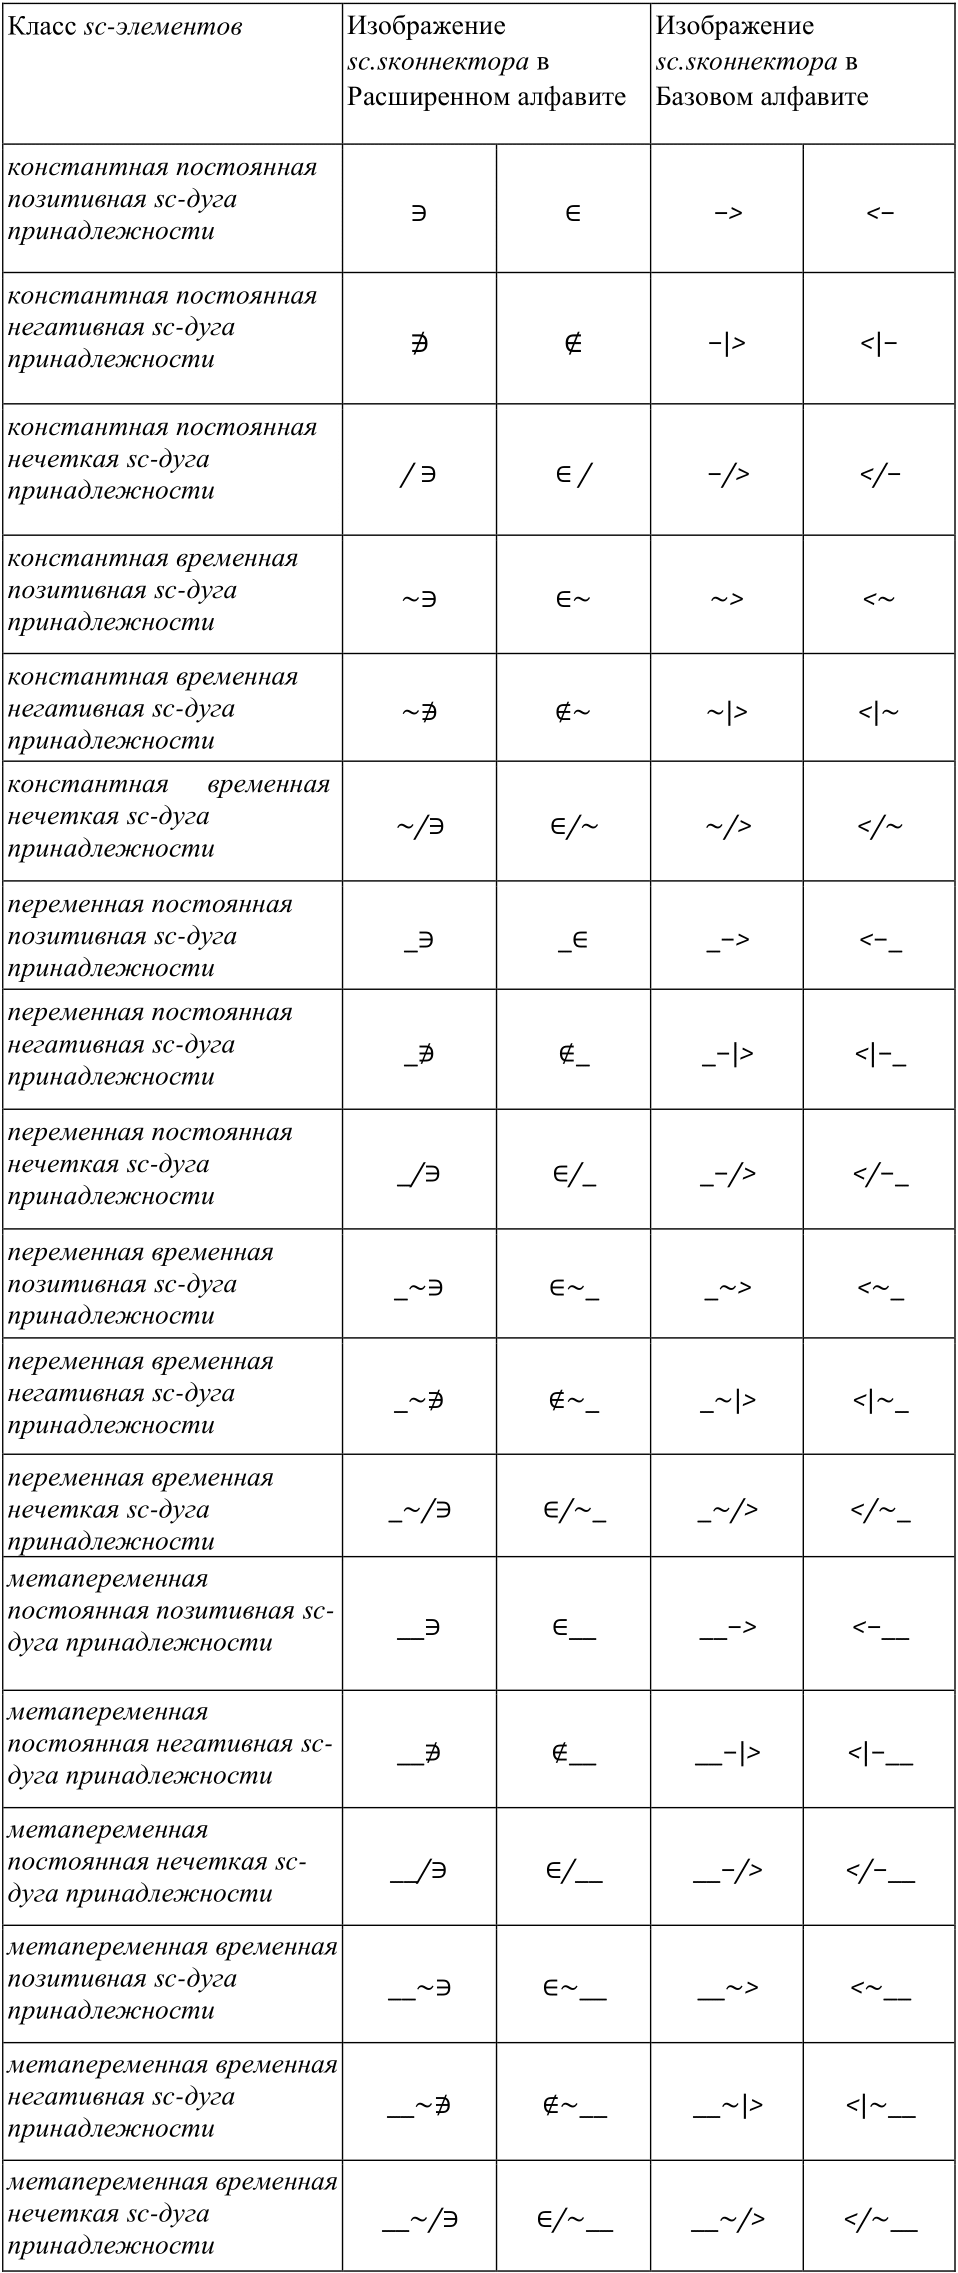
\includegraphics[scale=0.3]{images/intro/scs_membership_connectors_0.png}
\end{figure}

Знак равенства является \textit{sc.s-разделителем} двух \textit{sc-идентификаторов}, которые идентифицируют (именуют) одну и ту же сущность и, соответственно, являются \textit{sc-идентификаторами*} (внешними уникальными изображениями) одного и того же \textit{sc-элемента}. При этом из указанных двух sc-идентификаторов чаще всего один является простым \textit{sc-идентификатором}, а второй --- \textit{sc-выражением}. Реже оба эти \textit{sc-идентификатора} являются \textit{sc-выражениями}. И совсем редко оба они являются простыми sc-идентификаторами. Последнее обозначает то, что оба эти \textit{sc-идентификатора} являются основными \textit{sc-идентификаторами*} одного и того же \textit{sc-элемента}. Пример:
\textit{SC-код} = sc.s-текст;;

Здесь первый \textit{sc-идентификатор} является \textit{именем собственным}, а второй --- \textit{именем нарицательным}.

При трансляции \textit{sc.s-текста} в \textit{SC-код} знаку равенства на некотором этапе может быть поставлено в соответствие \textit{sc-ребро}, принадлежащее отношению \textit{синонимии}* \textit{sc-элементов}, идентифицируемых \mbox{\textit{sc-идентификаторами}}, связанными знаком равенства. Но на последующем этапе указанное \textit{sc-ребро} \uline{удаляется}, а связанные им \textit{sc-элементы} \uline{склеиваются}. Таким образом \textit{sc-ребро}, принадлежащее отношению \textit{синонимии}* sc-элементов, имеет не только денотационную, но и операционную семантику.

Знак равенства с включением --- изображение \textit{sc-дуги}, принадлежащей отношению погружения*, связывающей два \textit{sc-узла}, обозначающих \textit{sc-тексты}, первый из которых является погружающим, а второй (в который указанная \textit{sc-дуга} входит) является погружаемым, вводимым в состав первого \textit{sc-текста}. 

\textit{sc-дуга}, принадлежащая отношению погружения*, интерпретируется как команда погружения одного sc-текста в состав другого. При выполнении этой команды (1) все sc-элементы погружаемого \textit{sc-текста} становятся элементами, принадлежащими погружающему sc-тексту, (2) все синонимичные \textit{sc-элементы}, оказавшиеся в составе погружающего \textit{sc-текста}, склеиваются, (3) \textit{sc-узел}, обозначающий погружаемый \textit{sc-текст}, а так же спецификация этого \textit{sc-текста} (включая перечень всех его \textit{sc-элементов}) погружается в историю эволюции базы знаний вместе со спецификацией события погружения рассматриваемого \textit{sc-текста} в состав базы знаний.

Указанные \textit{sc.s-коннекторы} отличаются от остальных \textit{sc.s-коннекторов} тем, что они и соответствующие им sc-коннекторы (sc-ребра, принадлежащих отношению синонимии sc-элементов и sc-дуги, принадлежащие отношению погружения одного sc-текста в состав другого) имеют не только денотационную, но и операционную семантику, так как являются командами склеивания и командами погружения.

\bigskip
\textbf{\textit{Описание sc.s-предложений}}

\begin{SCn}
\scnheader{sc.s-предложение}
\scnidtf{минимальный семантически целостный фрагмент sc.s-текста}
\scnidtf{минимальный sc.s-текст}
\end{SCn}

\textit{sc.s-предложение}, (1) \uline{состоящее} или из двух \textit{sc-идентификаторов}, соединенных между собой \textit{\mbox{sc.s-коннектором}}, или из трех \textit{sc-идентификаторов}, разделенных \textit{sc.s-разделителями, изображающими связь инцидентности sc-элементов}, и (2) завершающееся \textit{двойной точкой с запятой}.

Нетрудно заметить, что простые sc.s-предложения по сути аналогичны триплетам языка RDF (\mbox{RDF-триплетам}), за тем исключением, что \textit{простое sc.s-предложение} можно "развернуть"{} при помощи \textit{Операции конверсии sc.s-предложений*} не меняя при этом его смысл, а RDF-триплет нельзя. Это является одной из причин, по которой, в отличие от RDF-триплетов, в простых \mbox{sc.s-предложениях} \textit{\mbox{sc.s-коннекторы}} и \textit{\mbox{sc.s-разделители}, изображающие связь инцидентности \mbox{sc-элементов}} не могут быть опущены, поскольку они в том числе показывают направление изображаемой ими связи между sc-элементами.

Признаком завершения любого \textit{sc.s-предложения}, то есть последними его символами является \textit{двойная точка с запятой}, которую, следовательно, можно считать разделителем \textit{sc.s-предложений}.

Выделяют следующие операции над sc.s-предложениями:
\begin{textitemize}
	\item \textbf{Операция конверсии sc.s-предложения*}
	
		Каждое \textit{sc.s-предложение} (в том числе, и \textit{простое sc.s-предложение}) можно преобразовать в семантически эквивалентное ему \textit{sc.s-предложение} путем конверсии ("разворота"{}) цепочки компонентов \textit{sc.s-предложения}. Так, например, при конверсии ("развороте") простого \textit{\mbox{sc.s-предложения}} (1) первый его \textit{\mbox{sc-идентификатор}} (первый компонент этого \textit{\mbox{sc.s-предложения}}) становится третьим компонентом конвертированного \textit{ \mbox{sc.s-предложения}}, (2) второй его \textit{\mbox{sc-идентификатор}} (третий компонент исходного \textit{\mbox{sc.s-предложения}}) становится первым компонентом "конвертированного"\ \textit{\mbox{sc.s-предложения}} и (3) второй компонент исходного \textit{\mbox{sc.s-предложения}} (\textit{\mbox{sc.s-коннектор}} или \textit{\mbox{sc.s-разделитель}, изображающий связь инцидентности \mbox{sc-элементов}}, соединяющий указанные выше компоненты) остается вторым компонентом конвертированного \textit{\mbox{sc.s-предложения}}, но меняет направленность ("$\ni$"\ заменяется на "$\in$"\ и наоборот, "$\supset$"\ на "$\subset$"\ и наоборот, "$\Rightarrow$"\ на "$\Leftarrow$"\ и наоборот и так далее).
	
	\item \textbf{Операция присоединения sc.s-предложения*}
		
		Операция соединения двух \textit{sc.s-предложений} при совпадении последнего компонента первого предложения с первым компонентом второго.
		В результате выполнения данной операции:
		\begin{textitemize}
			\item первый компонент второго \textit{sc.s-предложения} удаляется;
			\item оставшаяся часть второго предложения окружается \textit{sc.s-ограничителем} присоединенных предложений ("(*"{} и "*)"{}). Разделитель \textit{sc.s-предложений} (";;"{}) также попадает внутрь указанного ограничителя;
			\item полученная конструкция помещается между последним компонентом первого предложения и разделителем \textit{sc.s-предложений}, которым заканчивалось первое предложение;
			\item второе предложение, таким образом, становится \textit{присоединенным sc.s-предложением}.
		\end{textitemize}
	
		Аналогичным образом к любому присоединенному \textit{sc.s-предложению} могут "пристыковываться"\ другие присоединенные \textit{sc.s-предложения}, в общем случае уровень такой вложенности не ограничен.
		
		Присоединенные \textit{sc.s-предложения} используются для того, чтобы продолжить спецификацию какого-либо sc-элемента, \textit{sc-идентификатор} которого является последним компонентом в рамках какого-либо sc.s-предложения, не начиная при этом нового \textit{sc.s-предложения} и, таким образом, не дублируя указанный \mbox{sc-идентификатор}. Внутрь присоединенных sc.s-предложений также могут встраиваться другие присоединенные \textit{sc.s-предложения}, в общем случае уровень вложенности таких предложений не ограничен. Таким образом присоединенные \textit{sc.s-предложения} описывают "ветвление"{} \textit{sc.s-предложений}, при этом точками такого "ветвления"{} выступают \textit{sc-идентификаторы}, входящие в состав этих \textit{sc.s-предложений}.
		
		Благодаря введению \textit{присоединенных sc.s-предложений} появляется возможность любой \textit{sc-текст} изобразить в виде одного \textit{sc.s-предложения}, содержащего необходимое количество \textit{присоединенных sc.s-предложений}. Таким образом, \textit{SCs-код} по выразительной мощности становится эквивалентным \textit{SCn-коду}.
	
	\item \textbf{Операция слияния sc.s-предложений*}
		
		Операция присоединения \textit{простого sc.s-предложения} к \textit{sc.s-предложению}, у которого последний sc.s-коннектор совпадает с \textit{sc.s-коннектором} \textit{простого sc.s-предложения}, а предшествующий указанному \textit{sc.s-коннектору} sc-идентификатор совпадает с первым sc-идентификатором простого sc.s-предложения.
		
		В результате выполнения этой операции совпадающие sc-идентификаторы и sc.s-коннекторы соединяемых sc.s-предложений "склеиваются"{} , а последние sc-идентификаторы соединяемых \textit{sc.s-предложений} становятся последними компонентами объединенного \textit{sc.s-предложения},
		разделенными \textit{точкой с запятой}. Аналогичным образом можно присоединять сколько угодно простых \textit{sc.s-предложений}.
	
	\item \textbf{Операция разложения sc.s-предложений на простые sc.s-предложения*}
		
		Каждое \textit{sc.s-предложение} можно разложить на множество \textit{простых sc.s-предложений}, т.е. представить в виде последовательности \textit{простых sc.s-предложений}.
	
	\item \textbf{Операция разложения sc.s-предложений на простые sc.s-предложения с sc.s-разделителем, изображающим связь инцидентности sc-элементов*}
		
		Каждое \textit{sc.s-предложение} (в том числе и \textit{простое sc.s-предложение} с \textit{sc.s-коннектором}) можно представить в виде семантически эквивалентной последовательности \textit{простых \mbox{sc.s-предложений}} с \textit{sc.s-разделителем, изображающим связь инцидентности \mbox{sc-элементов}}.
		
		Данная операция осуществляет \uline{однозначное} (!) формирование множества \textit{простых \mbox{sc.s-предложений}} указанного вида.
\end{textitemize}

Операции, заданные на множестве \textit{sc.s-предложений} можно разделить на три группы:
\begin{textitemize}
	\item группа операций конверсии \textit{sc.s-предложений}, состоящая из одной операции;
	\item группа операций соединения \textit{sc.s-предложений};
	\item группа операций декомпозиции \textit{sc.s-предложений} и, в частности, операций разложения \textit{sc.s-предложений}.
\end{textitemize}

\bigskip
\textbf{\textit{компонент sc.s-предложения*}}

Каждое \textit{sc.s-предложение} представляет собой последовательность (1) \textit{sc-идентификаторов}, \mbox{(2) \textit{sc.s-коннекторов}} или \textit{sc.s-разделителей}, изображающих связь инцидентности \textit{sc-элементов}, (3) \textit{точек с запятыми}, (4) \textit{ограничителей присоединенных sc.s-предложений}, завершаемая \textit{двойной точкой с запятой}. При этом непосредственно соседствовать друг с другом не могут ни \textit{\mbox{sc-идентификаторы}}, ни \textit{\mbox{sc.s-коннекторы}}, ни, очевидно, \textit{точки с запятыми} и \textit{ограничители присоединенных sc.s-предложений}.\\
Между \textit{sc-идентификаторами} в рамках \textit{sc.s-предложения} может находиться либо \textit{точка с запятой}, либо \textit{sc.s-коннектор}, либо \textit{sc.s-разделитель}, изображающий связь инцидентности \textit{sc-элементов}. Слева и справа от \textit{sc.s-коннектора} и от \textit{sc.s-разделителя}, изображающего связь инцидентности \textit{sc-элементов}, должны находиться \textit{sc-идентификаторы}.

Указанные \textit{sc-идентификаторы}, \textit{sc.s-коннекторы} и \textit{sc.s-разделители}, изображающие связь инцидентности \textit{sc-элементов}, считаются компонентами соответствующего \textit{sc.s-предложения}. Понятие "быть компонентом sc.s-предложения"{} является относительным понятием (отношением), т.к. в состав некоторых компонентов \textit{sc.s-предложения} (в состав \textit{sc-идентификаторов}, являющихся \textit{sc.s-выражениями}, ограничиваемыми фигурными или квадратными скобками) могут входить других \textit{sc.s-предложения}, состоящие из своих компонентов.

\bigskip
\textbf{\textit{sc.s-модификатор*}}

Это дополнительный вид компонентов \textit{sc.s-предложений}. Каждый \textit{sc.s-модификатор}, являющийся компонентом некоторого \textit{sc.s-предложения}, представляет собой \textit{sc-идентификатор}, обозначающий множество (чаще всего, отношение), которому принадлежит sc-коннектор, изображенный \textit{sc.s-коннектором}, который предшествует указанному \textit{sc-идентификатору}. Признаком \textit{sc.s-модификатора} является \textit{двоеточие} (или \textit{двойное двоеточие}), которое ставится после \textit{sc.s-модификатора} и отделяет его либо от следующего за ним другого \textit{sc.s-модификатора} для этого же \textit{sc.s-коннектора}, либо от следующего за ним \textit{sc-идентификатора}, соответствующего sc-элементу, который инцидентен sc-коннектору, изображенному \textit{sc.s-коннектором}, находящимся левее рассматриваемого \textit{sc-идентификатора} после одного или нескольких \textit{sc.s-модификаторов}. Обычное ("одинарное"{}) \textit{двоеточие} обозначает, что sc-элемент, изображенный соответствующим \mbox{sc.s-модификатором}, связан с sc-коннектором, изображенным левее этого \mbox{sc.s-модификатора}, \textit{базовой \mbox{sc-дугой}} (\textit{константной постоянной позитивной \mbox{sc-дугой} принадлежности}), \textit{двойное двоеточие} обозначает, что указанные элементы связаны \textit{переменной постоянной позитивной \mbox{sc-дугой} принадлежности}.

\begin{SCn}
\scnheader{sc.s-текст}
\scnidtf{конкатенация \textit{sc.s-предложений}}
\scnidtf{последовательность \textit{sc.s-предложений}, разделяемых \textit{двойными точками с запятой}}
\end{SCn}

\textbf{\textit{sc.s-предложение}} является минимальным \textit{sc.s-текстом}. Смысл sc.s-текста (а также \textit{sc.s-текста, включенного в структуру} не зависит от порядка \textit{\mbox{sc.s-предложений}} в этих sc-текстах. Т.е. перестановка \textit{\mbox{sc.s-предложений}} в рамках таких \mbox{sc.s-текстов} смысла этих \mbox{sc.s-текстов} не меняет (т.е. приводит к семантически эквивалентным \mbox{sc.s-текстам}), но сильно влияет на трудоемкость человеческого восприятия (на "читабельность"{}) этих текстов.

\newpage
\subsection{Денотационная семантика SCs-кода}
\label{sec_scs_semantics}

\textbf{\textit{Таблица. Алфавит sc.s-коннекторов, соответствующих sc.g-дугам принадлежности\scnsupergroupsign}}
\begin{figure}[h]
	\centering
	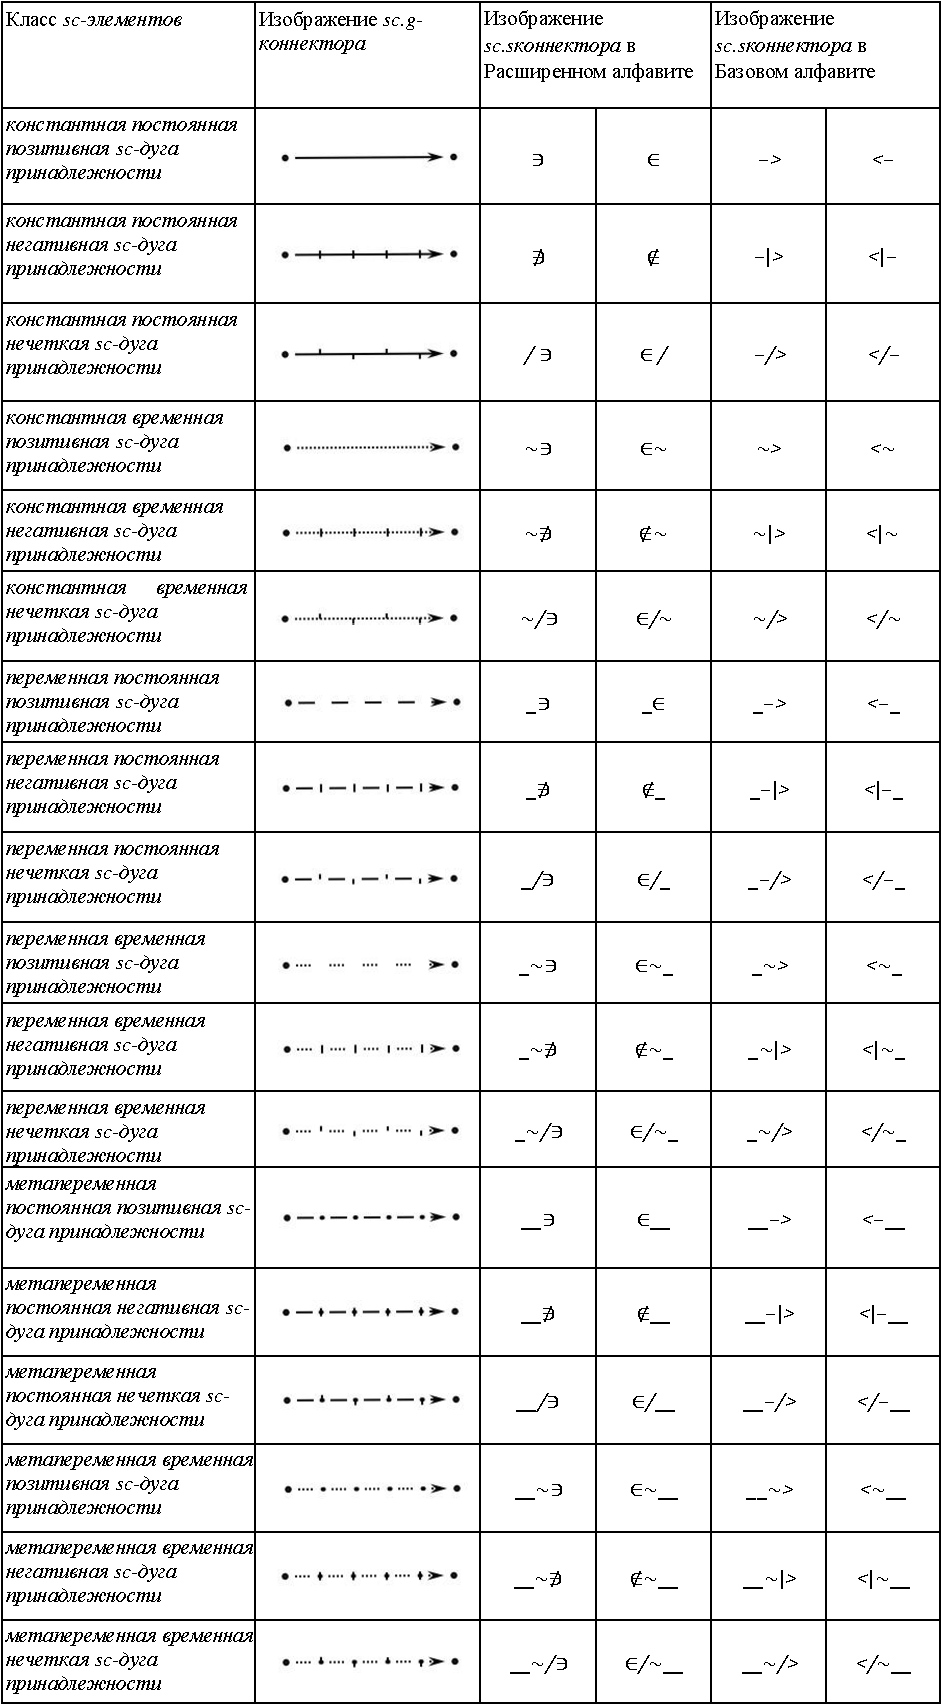
\includegraphics[scale=0.8]{images/intro/scs_membership_connectors.pdf}
\end{figure}

%---------------------------------------------

\textbf{\textit{Таблица. Алфавит sc.s-коннекторов, соответствующих sc.g-коннекторам, которые не являются sc.g-дугами принадлежности\scnsupergroupsign}}


\begin{figure}[h]
	\centering
	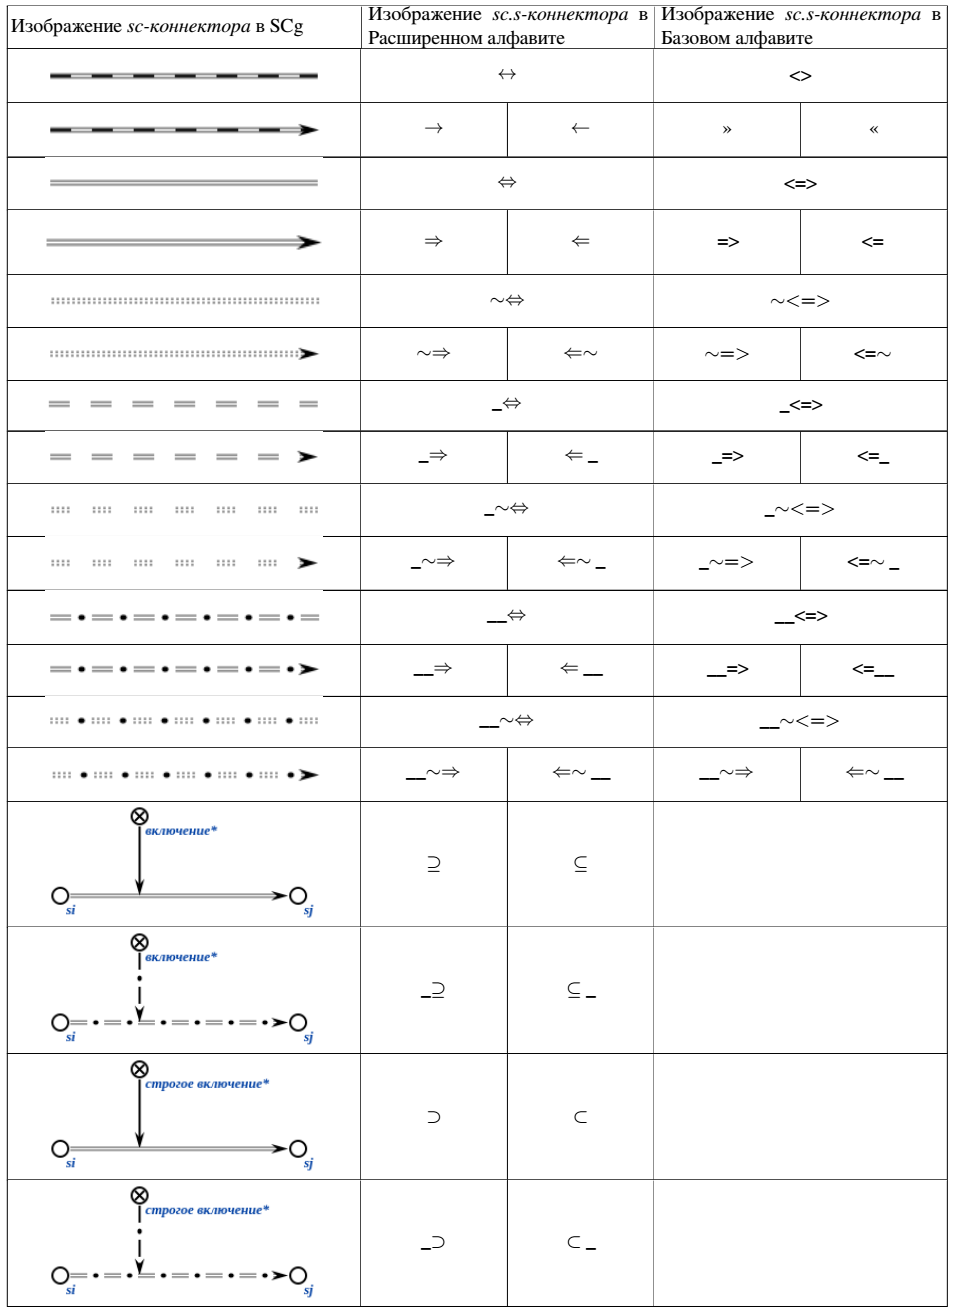
\includegraphics[scale=0.5]{images/intro/scs_non_membership_connectors_1.png}
\end{figure}

\begin{figure}[h]
	\centering
	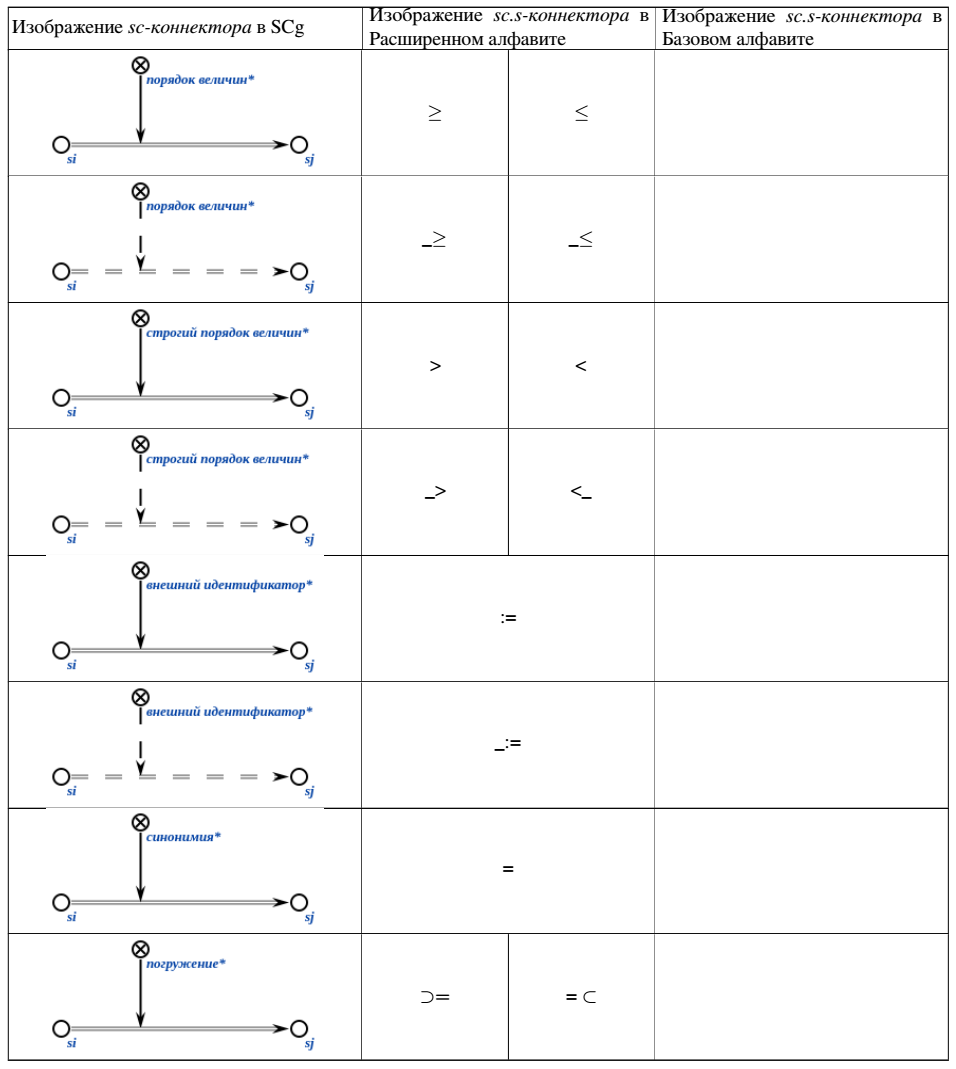
\includegraphics[scale=0.5]{images/intro/scs_non_membership_connectors_2.png}
\end{figure}

\newpage
\textbf{\textit{Примеры синтаксической трансформации sc.s-предложений с использованием Расширенного алфавита sc.s-коннекторов и соответствующие семантически эквивалентные конструкции в SCg-коде}}

\begin{SCn}
\scnfilelong{\textbf{\textit{si}}~$\Rightarrow$~\textit{включение*}:~\textbf{\textit{sj}}}
\scnrelfrom{синтаксическая трансформация}{
	\scnfilelong{\textbf{\textit{si}}~$\supseteq$~\textbf{\textit{sj}}}}
\begin{scnindent}
	\scnrelboth{семантическая эквивалентность}{
		\begin{figure}[h]
			\centering
			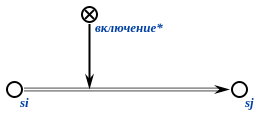
\includegraphics[scale=0.8]{images/intro/scs/sc.s-connectors/examples/scs_transf_inclusion_const.png}
	\end{figure}}
\end{scnindent}
\end{SCn}

\newpage

\begin{figure}[h]
	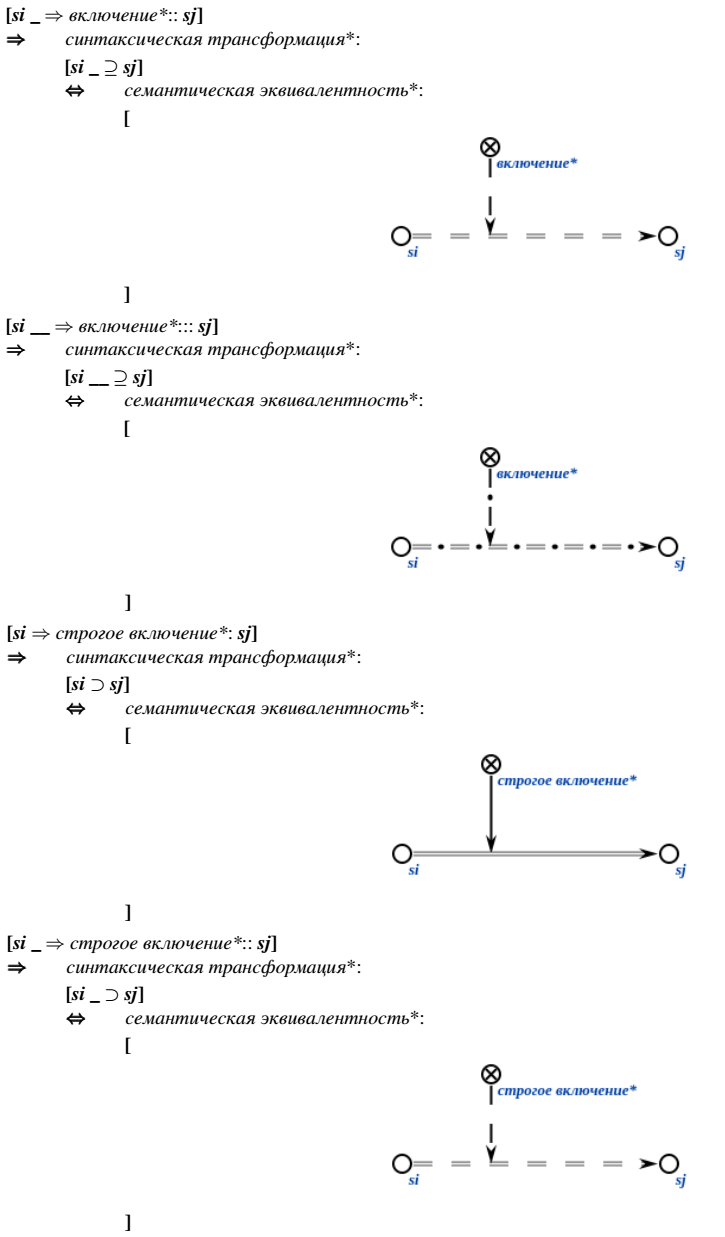
\includegraphics[scale=0.5]{images/intro/scs/sc.s-connectors/examples/example_1.png}
\end{figure}

\newpage
\begin{figure}[h]
	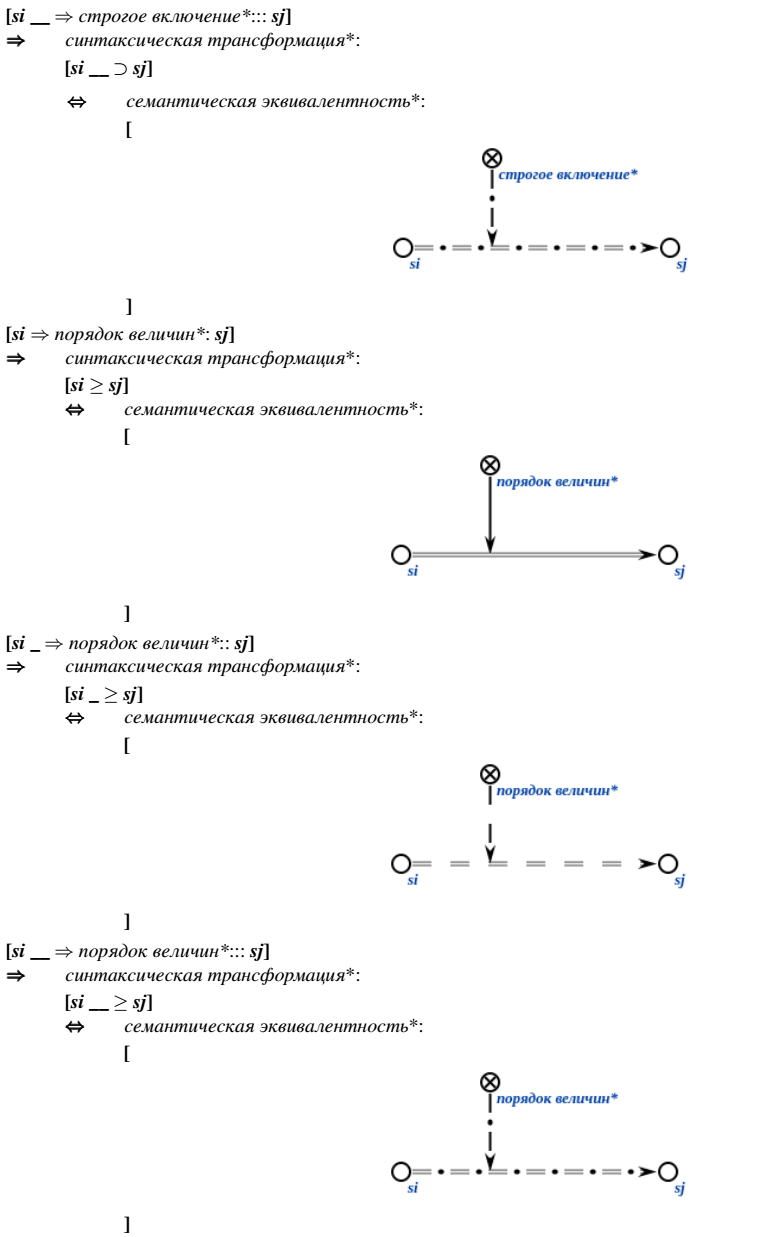
\includegraphics[scale=0.5]{images/intro/scs/sc.s-connectors/examples/example_2.png}
\end{figure}

\newpage
\begin{figure}[h]
	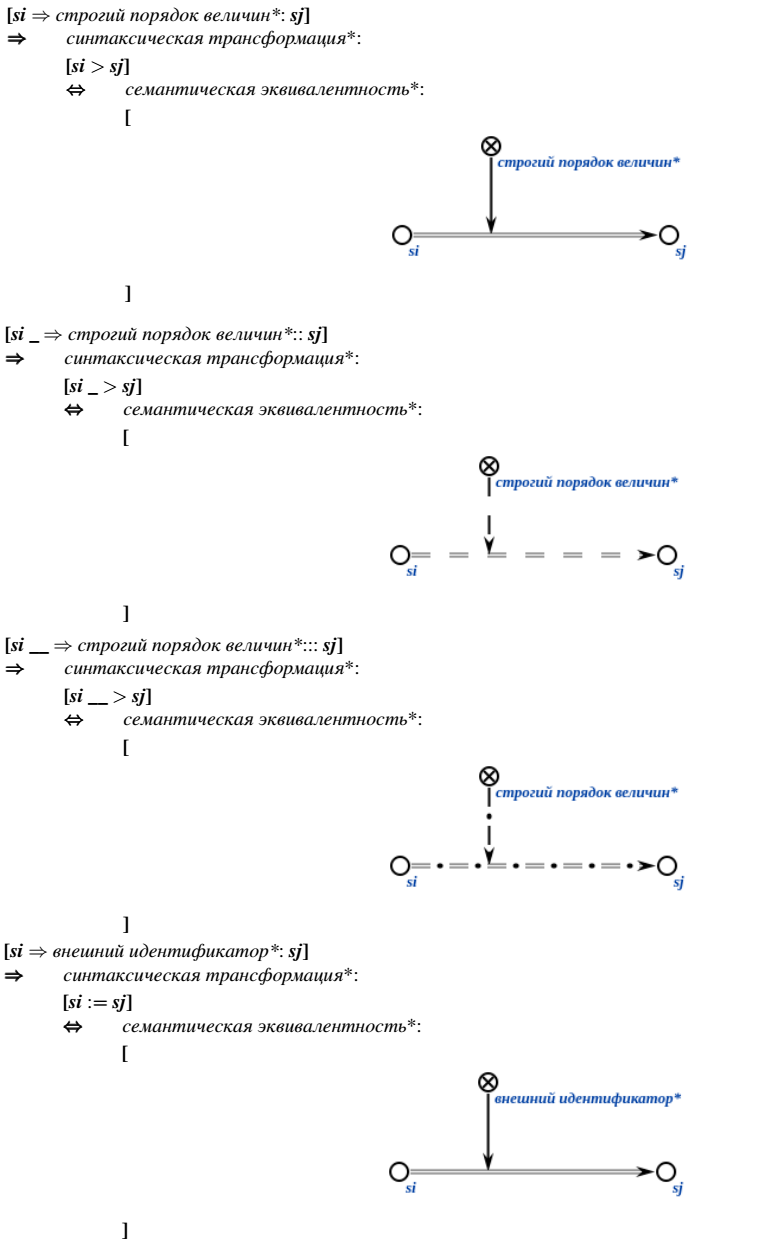
\includegraphics[scale=0.5]{images/intro/scs/sc.s-connectors/examples/example_3.png}
\end{figure}

\newpage
\begin{figure}[h]
	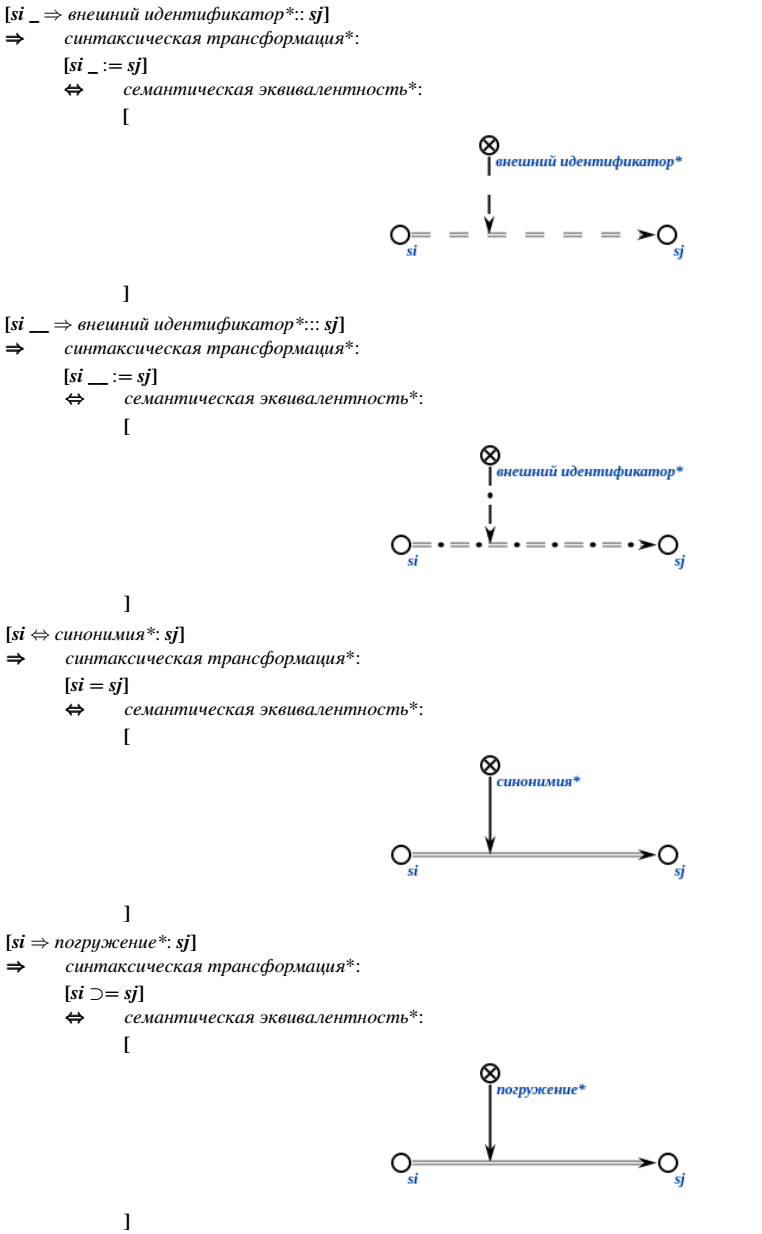
\includegraphics[scale=0.5]{images/intro/scs/sc.s-connectors/examples/example_4.png}
\end{figure}

Аналогичным образом может быть описана трансформация предложений, содержащих любые классы \textit{sc.s-коннекторов}, за исключением тех классов \textit{sc.s-коннекторов}, которые соответствуют классам \textit{sc-коннекторов}, входящим в \textit{Ядро SC-кода}.

В общем случае \textit{sc-элементы}, инцидентные \textit{sc-коннекторам}, классы которых описаны в данном примере, могут быть как \textit{sc-константами}, так и \textit{sc-переменными} (в том числе \textit{sc-метапеременными}). При этом как \textit{переменному sc-коннектору} может соответствовать \textit{константный sc-узел}, так и \textit{константному sc-коннектору} может соответствовать \textit{переменный sc-узел} (например, если возникает необходимость переменному sc-узлу приписать \textit{внешний идентификатор*}). Последняя ситуация встречается не очень часто и возникает в случае, когда область определения соответствующего \textit{отношения} имеет непустое пересечение с классом \textit{sc-переменных}.

\textbf{\textit{Описание примеров выполнения операций, заданных на множестве sc.s-предложений}}

С семантической точки зрения \textit{sc.s-предложение} представляет собой описание некоторого \uline{маршрута} в соответствующем sc-тексте, который является графовой структурой специального вида и структура которого описывается (изображается) с помощью \textit{sc.s-предложений}. Указанный маршрут "проводится"{} по sc-коннекторам и по связям инцидентности sc-элементов, если маршрут проходит через инцидентные sc-коннекторы. В описании указанного маршрута могут дополнительно указываться множества (чаще всего отношения), которым принадлежат sc-коннекторы, входящие в описываемый маршрут. Кроме того, указанный маршрут в начале и/или в конце может иметь разветвления, когда какой-либо sc-элемент \uline{одинаково} инцидентен нескольким \uline{однотипным} sc-коннекторам, соединяющим указанный sc-элемент с некоторыми другими sc-элементами.

Таким образом каждое указанное разветвление состоит из неограниченного числа ветвей, каждая из которых состоит из одного \textit{sc-коннектора} и одного связываемого им \textit{sc-элемента}.

\subsection{Иерархическое семейство подъязыков, семантически эквивалентных SCs-коду}
\label{sec_scs_extensions}

В рамках \textit{SCs-кода} выделяют \textit{Ядро SCs-кода} и \textit{Направления расширения Ядра SCs-кода}.

\begin{SCn}
\scnheader{Ядро SCs-кода}
\scnidtf{Подъязык \textit{SCs-кода}, который использует минимальный набор синтаксических средств, но при этом имеет семантическую мощность, эквивалентную мощности \textit{SCs-кода} в целом}
\end{SCn}

В \textit{Ядре SCs-кода}:
\begin{textitemize}
	\item используются только \textit{простые sc-идентификаторы}, в том числе \textit{sc-идентификаторы внешних файлов ostis-систем} (sc-выражения не используются);
	\item используются только \textit{sc.s-разделители, изображающие связь инцидентности sc-элементов}, а также sc.s-коннектор, изображающий константную  постоянную позитивную пару принадлежности ("$\in$"{} и "$\ni$"{} в Расширенном алфавите и "{}->{}"{} и "{}<-{}"{} в Базовом алфавите). Другие \textit{sc.s-коннекторы} не используются;
	\item не используются \textit{sc.s-модификаторы} и, соответственно, двоеточия, являющиеся признаком завершения \textit{sc.s-модификаторов};
	\item используются только \textit{простые sc.s-предложения}, которые, как следует из вышеуказанных свойств Ядра SCs-кода, либо состоят из двух \textit{простых sc-идентификаторов}, соединяемых sc.s-коннектором, изображающим константную  постоянную позитивную пару принадлежности, либо трех \textit{простых sc-идентификаторов}, разделенных \textit{sc.s-разделителями, изображающими связь инцидентности sc-элементов}.
\end{textitemize}

Из перечисленных свойств \textit{Ядра SCs-кода} следует, что для представления (изображения) любого \mbox{sc-текста} средствами \textit{Ядра SCs-кода} необходимо для \uline{всех} (!) sc-элементов этого \mbox{sc-текста} (кроме константных постоянных позитивных пар принадлежности) построить соответствующие им простые \textit{sc-идентификаторы}, то есть необходимо проименовать все указанные sc-элементы. В свою очередь, тип каждого используемого \mbox{sc-элемента} (кроме константных постоянных позитивных пар принадлежности) задается явно путем указания принадлежности этих элементов соответствующим классам sc-элементов, в том числе классам, входящим в \textit{Ядро SC-кода}.

Как видно из приведенного описания, \textit{Ядро SCs-кода} соответствует \textit{Ядру SCg-кода}, за исключением того, что в \textit{Ядре SCg-кода} нет необходимости именовать все изображаемые \textit{sc-элементы}, а также в\textit{ Ядре SCg-кода} присутствуют графические изображения для sc-элементов, принадлежащих соответствующим классам \textit{Ядра SC-кода} и эту принадлежность нет необходимости указывать явно.

Очевидно, что широко практически применять \textit{Ядро SCs-кода} для записи больших фрагментов баз знаний неудобно и неэффективно. Тем не менее, с практической точки зрения \textit{Ядро SCs-кода} может использоваться, например, для обмена информацией со сторонними средствами представления графовых конструкций, рассчитанными на представление информации в виде триплетов (например, RDF-хранилищ).
Для обеспечения возможности более широкого практического использования необходимы синтаксические расширения \textit{Ядра SCs-кода} в целях:
\begin{textitemize}
	\item минимизации числа идентифицируемых (именуемых) sc-элементов путем использования \textit{sc-выражений} и ликвидации необходимости идентифицировать (именовать) \uline{все} (!) \textit{sc-элементы};
	\item сокращения текста путем минимизации числа повторений одного и того же \textit{sc-идентификатора} путем соединения \textit{sc.s-предложений};
	\item повышение уровня наглядности, "читабельности"{} \textit{sc.s-текстов}.
\end{textitemize}

\begin{SCn}
\scnheader{Первое направление расширения Ядра SCs-кода}
\scnidtf{Первое направление расширения Ядра SCs-кода \uline{и всех иных его расширений}}
\end{SCn}

По сравнению с \textit{Ядром SCs-кода} в \textit{Первом направлении расширения Ядра SCs-кода} вместо \textit{sc-идентификато|-ров}, являющихся идентификаторами (именами), которые взаимно однозначно соответствуют синонимичным им (представляемым ими) sc-коннекторам, вводятся \textit{sc.s-коннекторы}, каждый из которых соответствует не одному конкретному sc-коннектору, а некоторому классу однотипных sc-коннекторов. Очевидно, что это ликвидирует необходимость \uline{каждому} sc-коннектору приписывать уникальный \textit{sc-идентификатор}. Кроме того, \textit{Алфавит sc.s-коннекторов\scnsupergroupsign} включает в себя элементы этого Алфавита (классы \uline{синтаксически} эквивалентных \textit{sc.s-коннекторов}), которые соответствуют \uline{всем} (!) элементам \textit{Алфавита sc-коннекторов\scnsupergroupsign}, но при этом дополнительно включают в себя и другие элементы \textit{Алфавита sc.s-коннекторов\scnsupergroupsign}, которые соответствуют часто используемым \uline{семантически} явно выделяемым классам sc-коннекторов. К таким дополнительно вводимым классам \textit{sc.s-коннекторов} относятся \textit{константные sc.s-коннекторы} включения множеств ("$\supset$"{} или "$\subset$"{}), \textit{переменные sc.s-коннекторы} включения множеств ("$\_\supset$"{} или "$\subset\_$"{}), \textit{sc.s-коннектор} синонимии ("$=$"{}), \textit{sc.s-коннектор} погружения ("$=\subset$"{} или "$\supset=$"{}) и другие.

Заметим, что указанное расширение \textit{Алфавита SCs-кода\scnsupergroupsign} \textit{sc.s-коннекторов} аналогично расширенному Алфавиту \textit{sc.g-коннекторов} в SCg-коде и ликвидирует необходимость (как и в SCs-коде) явно специфицировать (средствами SCs-кода) синтаксически выделяемые классы \textit{sc.s-коннекторов}.

\textbf{\textit{Второе направление расширения Ядра SCs-кода}}

Во \textit{Втором направлении расширения Ядра SCs-кода} вводятся модификаторы \textit{sc.s-коннекторов} (\textit{\mbox{sc.s-модификаторы}}), которые позволяют достаточно компактно дополнительно специфицировать \mbox{sc-коннекторы}, изображаемые (представляемые) соответствующими \textit{sc.s-коннекторами}. Речь идет о такой часто востребованной форме спецификации sc-коннекторов, как указание множества (возможно, нескольких множеств), которому принадлежит специфицируемый  sc-коннектор (чаще всего, таким множеством является \textit{бинарное отношение} (в частности, \textit{ролевое отношение}) или \textit{квазибинарное отношение}).

\begin{SCn}
\scnheader{sc.s-модификатор*}
\scniselement{отношение}
\begin{scnindent}
	\scnidtf{относительное понятие}
\end{scnindent}	
\scnidtf{модификатор sc.s-коннектора*}
\textit{sc-идентификатор}, который (1) находится либо между \textit{sc.s-коннектором} и \textit{двоеточием}, либо между \textit{двоеточиями} и (2) обозначает множество (чаще всего, отношение), которому принадлежит sc-коннектор, изображаемый ближайшим предшествующим \textit{sc.s-коннектором}. Два подряд идущих двоеточия ("::"{}) обозначают, что указанное множество связано с указанным sc-коннектором \textit{\uline{переменной} позитивной постоянной sc-дугой принадлежности}.
\end{SCn}

Очевидно, что, если не использовать \textit{sc.s-модификаторы}, указанного вида спецификация sc-коннекторов средствами SCs-кода будет выглядеть значительно более громоздкой.

\textbf{\textit{Третье направление расширения Ядра SCs-кода}}

В \textit{Третьем направлении расширения Ядра SCs-кода} осуществляется переход от использования только \textit{простых sc-идентификаторов} к использованию как \textit{простых sc-идентификаторов}, так и \textit{sc-выражений}, а также к использованию \textit{sc.s-представлений некоторых неидентифицируемых sc-узлов}. Это существенно сокращает число придумываемых \textit{простых sc-идентификаторов}, т.к. каждое \textit{sc-выражение} в конечном счете — это комбинация \textit{простых sc-идентификаторов}, построенная по правилам, которые достаточно легко семантически интерпретируются. Если проводить аналогию с SCg-кодом, то очевидно, что \textit{\mbox{sc-выражение}}, ограничиваемое фигурными скобками, есть не что иное, как информационная конструкция, ограничиваемая \textit{sc.g-контуром}, а \textit{sc-выражение}, ограничиваемое квадратными скобками есть не что иное, как информационная конструкция, ограничиваемая \textit{sc.g-рамкой}. Отличие здесь заключается в том, что круглыми и квадратными скобками можно ограничивать только линейные информационные конструкции (цепочки символов).

\begin{SCn}
\scnheader{sc.s-представление неидентифицируемого sc-узла}
\scnidtf{изображение (представление) неидентифицируемого (неименуемого) sc-узла в sc.s-тексте}
\scnidtf{sc.s-обозначение неименуемой сущности, не являющейся парой, обозначаемой sc-коннектором}
\scnidtf{sc.s-представление sc-узла, не являющееся sc-идентификатором (именем этого sc-узла)}
\end{SCn}

Если одно и то же обозначение неименуемой сущности встречается в \uline{разных} \textit{sc.s-предложениях}, то считается, что это обозначения \uline{разных} сущностей, т.е. изображения \uline{разных} sc-узлов.

\textbf{\textit{Четвертое направление расширения Ядра SCs-кода}}

В \textit{Четвертом направлении расширения Ядра SCs-кода} осуществляется переход от использования только \textit{простых sc.s-предложений} к использованию также \textit{sc.s-предложений}, построенных с помощью \textit{\mbox{Операции} присоединения sc.s-предложения*}. В результате этого, благодаря "склеиванию"{} одинаковых \textit{\mbox{sc-идентификаторов}}, а также "склеиванию"{} синтаксически эквивалентных \textit{\mbox{sc.s-коннекторов}} с одинаковыми \textit{\mbox{sc.s-модификаторами}} (несмотря на то, что эти "склеиваемые"{} \textit{sc.s-коннекторы} соответствуют \uline{разным} \mbox{sc-коннекторам}), существенно сокращается число копий используемых \textit{\mbox{sc-идентификаторов}} и \textit{\mbox{sc.s-коннекторов}} с их \textit{\mbox{sc.s-модификаторами}}.

\textbf{\textit{Пятое направление расширения Ядра SCs-кода}}

В \textit{Пятом направлении расширения Ядра SCs-кода} разрешается использование \textit{присоединенных \mbox{sc.s-предложений}}. В результате этого \textit{sc.s-тексты} становятся более компактными и удобными для восприятия за счет снижения числа дублируемых \textit{sc-идентификаторов} и более широких возможностей их структуризации.

\section{Язык внешнего форматированного представления конструкций SC-кода --- SCn-код (Semantic Code natural)}
\label{sec_scn}

\begin{SCn}
\begin{scnrelfromlist}{подраздел}
	\scnitem{\ref{sec_scn_syntax}~\nameref{sec_scn_syntax}}
	\scnitem{\ref{sec_scn_semantics}~\nameref{sec_scn_semantics}}
	\scnitem{\ref{sec_scn_latex}~\nameref{sec_scn_latex}}
\end{scnrelfromlist}

\begin{scnrelfromlist}{ключевое понятие}
	\scnitem{страница sc.n-текста}
	\scnitem{строка sc.n-текста}
	\scnitem{линия разметки sc.n-текста}
	\scnitem{sc.n-предложение}
	\scnitem{sc.n-элемент}
	\scnitem{sc.n-коннектор}
	\scnitem{sc.n-ребро}
	\scnitem{sc.n-дуга}
	\scnitem{sc.n-контур}
	\scnitem{sc.n-рамка}
\end{scnrelfromlist}

\begin{scnrelfromlist}{ключевой знак}
	\scnitem{SCn-код}
	\scnitem{Алфавит SCn-кода\scnsupergroupsign}
	\scnitem{Синтаксис SCn-кода}
	\scnitem{Денотационная семантика SCn-кода}
\end{scnrelfromlist}
\end{SCn}

\begin{SCn}
\scnheader{SCn-код}
\scnidtf{Язык структурированного представления знаний \textit{ostis-систем}}
\scnidtf{Язык внешнего форматированного представления конструкций внутреннего языка ostis-систем}
\end{SCn}

\textbf{\textit{SCn-код}} является языком структурированного внешнего представления текстов \textit{SC-кода} и представляет собой синтаксическое расширение \textit{SCs-кода}, направленное на повышение наглядности и компактности текстов \textit{SCs-кода}. 

\textit{SCn-код} позволяет перейти от линейных текстов \uline{SCs-кода} к форматированным и фактически двухмерным текстам, в которых появляется декомпозиция исходного линейного текста \uline{SCs-кода} на \uline{строчки}, размещенные "по вертикали"{}. При этом начало всех \uline{строчек} текста фиксировано и определяется известным и ограниченным набором правил, что дает возможность использовать это при форматировании \uline{sc.n-текста} (текста, принадлежащего \textit{SCn-коду}).

\subsection{Синтаксис SCn-кода}
\label{sec_scn_syntax}

\textit{Алфавит SCs-кода\scnsupergroupsign} является также алфавитом символов и \textit{SCn-кода}, то есть \textit{алфавиты}* этих языков совпадают.

\textit{SCn-код} --- язык, каждый \textit{текст} которого задается:
\begin{textitemize}
	\item множеством входящих в него \textit{символов};
	\item отношением порядка (последовательности) \textit{символов} по "горизонтали"{};
	\item отношением порядка(последовательности) \textit{символов} по "вертикали"{}.
\end{textitemize}

\begin{SCn}
	\scnheader{sc.n-текст}
	\scnidtf{текст SCn-кода}
	\scnidtf{последовательность предложений SCn-кода}
	\scnidtf{последовательность предложений SCn-кода, каждое из которых не является частью какого-либо другого предложения из \uline{этой} последовательности}
\end{SCn}

Важной особенностью \textit{SCn-кода} является "двухмерный"{} характер его текстов. Это проявляется в том, что для каждого фрагмента текста \textit{SCn-кода} важное значение имеет величина отступа от левого края \textit{строчки}.

Символ, входящий в состав \textit{двухмерного текста}, в общем случае может иметь четыре "соседних"{} \textit{символа}: 
\begin{textitemize}
	\item \textit{символ}, находящийся от него \uline{слева} в рамках той же \textit{строчки};
	\item \textit{символ}, находящийся от него \uline{справа} в рамках этой же \textit{строчки};
	\item \textit{символ}, находящийся строго \uline{над} ним в предыдущей \textit{строчке};
	\item \textit{символ}, находящийся строго \uline{под ним} в следующей \textit{строчке} текста.
\end{textitemize}

Благодаря тому, что в состав \textit{sc.n-текстов} могут входить и \textit{sc.s-тексты}, и \textit{sc.g-тексты} (ограниченные \textit{sc.n-контуром}), SCn-код можно считать интегратором различных внешних языков представления знаний.  Это дает возможность при визуализации и разработке базы знаний ostis-системы недостатки одного из предлагаемых вариантов внешнего представления sc-текстов (\textit{SCg-кода}, \textit{SCs-кода}, \textit{SCn-кода}) компенсировать достоинствами других вариантов.

\begin{SCn}
\scnheader{страница sc.n-текста}
\scnidtf{страница, на которой размещается sc.n-текст}
\end{SCn}

Если \textit{sc.n-текст} является частью какого-либо другого файла, разделяемого на страницы, например, публикации какой-либо части базы знаний, то \textit{sc.n-страницей} считается только часть страницы, на которой изображен \textit{sc.n-текст}, в то время как страница указанного файла может быть больше за счет, например, белых полей по краям страницы, необходимых для последующей распечатки.

\textbf{\textit{строчка sc.n-текста}}

Максимальное количество символов в строчках \textit{sc.n-текста} для каждого \textit{sc.n-текста} фиксировано и определяется конкретным вариантом размещения \textit{sc.n-текста}. При этом, в зависимости от отступов в рамках конкретного \textit{sc.n-предложения}, строчка \textit{sc.n-текста} может начинаться не с левого края \textit{sc.n-текста} (но всегда с какой-то из вертикальных линий разметки) и иметь произвольную длину, ограничиваемую правой границей \textit{sc.n-страницы}.

\begin{SCn}
\scnheader{линия разметки sc.n-текста}
\scnidtf{табуляционная линия sc.n-текста}
\scnidtf{вертикальная линия разметки sc.n-текста}
\scnidtf{вертикальная табуляционная линия}
\scnidtf{вертикальная линия, используемая для упрощения восприятия sc.n-текстов и показывающая уровень отступа для компонентов sc.n-предложений}
\end{SCn}

1-я линия разметки ограничивает левый край \textit{sc.n-страницы}, 2-я линия разметки располагается примерно между 5 и 6 символами строчки и так далее. Расстояние между линиями разметки может меняться в зависимости от размера шрифта, однако в рамках одного \textit{sc.n-текста} всегда остается одинаковым. Общее количество линий разметки ограничивается максимально возможной шириной \textit{sc.n-страницы} в конкретном файле \textit{ostis-системы}, содержащем данный \textit{sc.n-текст}.

\begin{SCn}
\scnheader{следует отличать*}
\begin{scnhaselementset}
	\scnitem{страница sc.n-текста}
	\scnitem{строчка sc.n-текста}
	\scnitem{строка}	
\end{scnhaselementset}
\end{SCn}

Все компоненты \textit{sc.s-текстов} используются также и в \textit{sc.n-текстах}:
\begin{textitemize}
	\item \textit{sc-идентификаторы};
	\item \textit{sc.s-коннекторы};
	\item модификаторы \textit{sc.s-коннекторов} с соответствующими разделителями (двоеточиями)
	\item разделители, используемые в sc-выражениях, обозначающих sc-множества, заданные перечислением элементов с соответствующими разделителями (\textit{точкой с запятой} или \textit{круглым маркером});
	\item \textit{круглые маркеры} в перечислениях идентификаторов \mbox{sc-элементов}, связанных однотипными sc-коннекторами с однотипными модификаторами с заданным sc-элементом;
	\item разделители предложений (двойные точки с запятой) (опускаются при преобразовании \mbox{sc.s-предложений} в \mbox{sc.n-предложения});
	\item ограничители присоединенных \textit{sc.s-предложений} (опускаются при преобразовании sc.s-предложений в sc.n-предложения).
\end{textitemize}

В отличие от \textit{sc.s-текстов} в \textit{sc.n-текстах}:
\begin{textitemize}
	\item добавляются новые виды \textit{sc-выражений} (а именно --- sc-выражений, имеющих двухмерный характер);
	\item добавляется новый вид разделителей предложений --- пустая строчка;
	\item меняется размещение предложений с учетом двухмерного характера такого размещения.
\end{textitemize}

В \textit{SCn-коде} по сравнению с \textit{SCs-кодом} добавляются новые виды \textit{sc-выражений}:
\begin{textitemize}
	\item \textit{sc-выражение}, представляющее собой двухмерный \textit{\mbox{sc.n-текст}}, ограниченный \textit{sc.n-контуром} или \textit{sc.n-рамкой}. Каждый \textit{sc.n-контур} изображается условно в виде \textit{открывающей фигурной скобки} и расположенной строго \uline{под} ней через несколько строчек \textit{закрывающей фигурной скобки}. Внутри указанных скобок (начиная от линии вертикальной разметки, на которой расположены сами скобки, и до правого края \textit{страницы}) размещается sc.n-текст. Полученный sc.n-контур является изображением структуры, являющейся результатом трансляции указанного sc.n-текста в SC-код. Каждая \textit{sc.n-рамка} изображается аналогичным образом, только вместо \textit{фигурных скобок} в ней используются \textit{квадратные скобки}, либо \textit{квадратные скобки} с \textit{восклицательным знаком} (в случае файла-образца);
	\item \textit{sc-выражение}, представляющее собой двухмерный \textit{sc.g-текст}, ограниченный \textit{\mbox{sc.n-контуром}} или \textit{\mbox{sc.n-рамкой}}.
	\item \textit{sc-выражение}, представляющее собой ограниченное \textit{sc.n-рамкой} двухмерное графическое изображение \textit{информационной конструкции}, закодированной в некотором \textit{файле ostis-системы}. Такой \textit{информационной конструкцией} может быть таблица, рисунок, фотография, диаграмма, график и многое другое.
\end{textitemize}

Нетрудно заметить, что \textit{sc.n-контур} является, по сути, двухмерным эквивалентом \textit{sc-выражения структуры}, а \textit{sc.n-рамка} --- двухмерным эквивалентом \textit{sc-выражения внутреннего файла \mbox{ostis-системы}} или \textit{sc-выражения, обозначающего файл-образец ostis-системы}.

\begin{SCn}
\scnheader{sc.n-рамка}
\scnidtf{ограничитель изображения файла \uline{ostis-системы}, используемый в \uline{sc.n-предложениях}}
\end{SCn}

Обозначается с помощью квадратных скобок: `` [ '', `` ] ''.

С формальной точки зрения \textit{sc.n-рамка} всегда представляет собой \uline{одну} \textit{строчку sc.n-текста}. Это означает, что \textit{sc.n-рамка} не может быть синтаксически разделена на части в рамках того \textit{sc.n-текста}, в котором она используется, и внутрь нее не могут вставляться, например, \textit{присоединенные sc.n-предложения} или какой-либо другой текст (за исключением случаев, когда \textit{sc.n-рамка} содержит \textit{sc.n-текст}, но в этом случае указанный \textit{sc.n-текст} все равно будет рассматриваться как целостный внешний файл, а не как фрагмент окружающего его \textit{sc.n-текста}). 

\begin{SCn}
	\scnheader{sc.n-контур}
	\scnidtf{используемый в sc.n-предложениях ограничитель, являющийся изображением структуры}
\end{SCn}

Обозначается с помощью фигурных скобок: `` \{ '', `` \} ''.

Понятие \textbf{\textit{sc.n-предложения}} является естественным обобщением понятия \textit{sc.s-предложения}. Более того, аналогичным для \textit{sc.s-предложений} образом вводятся понятия:
\begin{textitemize}
	\item \textit{простого sc.n-предложения}
	\item \textit{сложного sc.n-предложения}
	\item \textit{sc.n-предложения, содержащего присоединенные sc.n-предложения}
	\item \textit{sc.n-предложения, не содержащего присоединенные sc.n-предложения}
	\item \textit{присоединенного sc.n-предложения}
	\item \textit{неприсоединенного sc.n-предложения}
\end{textitemize}

\uline{Если} каждое \textit{неприсоединенное sc.s-предложение} \uline{либо} являетcя первым предложением \textit{sc.s-текста}, \uline{либо} начинается после \textit{разделителя sc.s-предложений} (\textit{двойной точки с запятой}), \uline{то} каждое \textit{неприсоединенное sc.n-предложение} начинается с начала новой строчки.

\uline{Если} каждое \textit{присоединенное sc.s-предложение} начинается либо после открывающего ограничителя присоединенных sc.s-предложений (открывающей круглой скобки со звездочкой), \uline{либо} после \textit{разделителя sc.s-предложений}, \uline{то} каждое \textit{присоединенное sc.n-предложение} начинается с новой строчки под sc-идентификатором, которым завершается то sc.n-предложение (и соответственно, sc.s-предложение), в которое встраивается данное \textit{присоединенное sc.n-предложение}.

Первый \textit{sc-идентификатор}, входящий в состав \textit{sc.n-предложения} до \textit{sc.s-коннектора} выделяется \uline{жирным} курсивом;
В \textit{sc.n-предложениях двойная точка с запятой} не используется в качестве признака завершения этих предложений и, соответственно, не используется в качестве разделителя \textit{sc.n-предложений}. Таким разделителем является \textit{пустая строчка}.

Благодаря двухмерности \textit{SCn-кода} появляются более широкие возможности (степени свободы) для наглядного и компактного размещения \textit{sc.n-предложений}.

При оформлении \textit{sc.n-предложения} осуществляется четкая \uline{табуляция} всех присоединенных к нему \textit{sc.n-предложений}, присоединяемых к исходному "по вертикали"{}. Вертикальная линия табуляции задает левую границу исходного (максимального) sc.n-предложения или левую границу присоединенного \textit{sc.n-предложения}, присоединяемого "по вертикали". Левая граница sc.n-предложения задает начало первого sc-идентификатора, входящего в состав этого \mbox{sc.n-предложения}, а также начало \textit{sc.s-коннектора}, инцидентного указанному \mbox{sc-идентификатору} и размещаемого \uline{строго под} этим \textit{sc-идентификатором}. Расстояние между вертикальными табуляционными линиями фиксировано и примерно равно максимальной длине \textit{sc.s-коннектора}.

\subsection{Денотационная семантика SCn-кода}
\label{sec_scn_semantics}

В отличие от \textit{sc.s-текстов}: в \textit{sc.n-текстах} \textit{sc.s-коннектор} может быть инцидентен предшествующему sc-идентификатору (как простому, так и \textit{sc-выражению}) не только "по горизонтали"{}, но и "по вертикали"{}. Для этого \textit{sc.s-коннектор} размещается строго \uline{под} предшествующим ему sc-идентификатором.

Кроме того "по вертикали"\ sc-идентификатор может быть инцидентен не одному, а \uline{нескольким} \textit{sc.s-коннекторам}, которые последовательно "по вертикали"{} размещаются \uline{под} указанным \textit{sc-идентификатором}. Это позволяет в рамках одного \textit{sc.n-предложения} представлять произвольное число "ответвлений"{} от каждого sc-идентификатора, то есть произвольное число \textit{sc.s-коннекторов}, инцидентных этому \textit{sc-идентификатору};
Каждый \textit{sc-идентификатор}, включая \textit{sc-выражение}, ограничиваемого фигурными или квадратными скобками, должен размещаться сразу правее вертикальной разметочной линии, если \uline{под ним} размещается \textit{sc.s-коннектор}.

Каждый \textit{sc.s-коннектор} выделяется жирным некурсивным шрифтом и, если он находится \uline{под} инцидентным ему \textit{sc-идентификатором}, размещается строго между двумя вертикальными разметочными линиями, прижимаясь при этом к левой из этих двух разметочных линий.

Поскольку по отношению к \textit{SCn-коду} \textit{SCs-код} является \textit{синтаксическим ядром языка*}, \textit{SCn-код} можно рассматривать как результат интеграции нескольких направлений расширения \textit{SCs-кода}, в основе которых лежат правила синтаксической трансформации \textit{sc.s-текстов} и \textit{sc.n-текстов}, ориентированные на повышение эффективности использования тех возможностей обеспечения наглядности и компактности \textit{sc.n-текстов}, которые открываются при переходе от линейности \textit{sc.s-текстов} к двухмерности \textit{sc.g-текстов}.

\subsection{Язык представления исходных текстов баз знаний на основе языка LaTeX}
\label{subsec_LaTeX}

Одним из удобных вариантов представления исходных текстов баз знаний для различных областей научно-технической деятельности является Язык представления исходных текстов баз знаний на основе языка LaTeX. В его основу положен язык LaTeX, так как:
\begin{textitemize}
	\item LaTeX это популярный общепринятый язык для записи научно-технических текстов;
	\item LaTeX представляет собой достаточно мощный и легко расширяемый язык;
	\item LaTeX это достаточно строгий и формальный язык, что позволяет реализовать для него транслятор исходных текстов в базу знаний интеллектуальной системы.
\end{textitemize}

Язык представления исходных текстов баз знаний на основе языка LaTeX был разработан для:
\begin{textitemize}
	\item формирования читабельного текста для публикации всего текста \textit{Стандарта OSTIS} или фрагментов в виде печатных изданий;
	\item возможности иметь формальный исходный текст \textit{Стандарта OSTIS}, который может быть протранслирован в базу знаний.
\end{textitemize}

Предлагаемый набор команд условно называется scn-tex (см. \scncite{Ostis-scn-LaTeX-plugin2023}), поскольку в его основу положена идея того, чтобы разработчик писал исходный текст максимально приближенно к тому, как он будет видеть результат компиляции этого исходного текста в SCn-коде и при этом максимально был избавлен от необходимости учитывать особенности языка LaTeX в работе.

Основные принципы разработки исходных текстов баз знаний с использованием scn-tex:
\begin{textitemize}
	\item весь исходный текст стандарта формируется исключительно с использованием набора команд scn-tex;
	\item запрещается использовать любые другие команды для форматирования текста, изменения шрифта, вставки внешних файлов и т.д;
	\item в рамках естественно-языковых фрагментов, входящих в состав стандарта, допускается использование команд LaTeX для вставки специальных символов и математических формул
	\item для добавления файлов изображений в текст стандарта используются только команды scn-tex;
	\item используются для формирования нумерованных и маркированных списков, добавления закрывающих и открывающих скобок различного вида (кроме круглых) используются только команды scn-tex;
	\item для выделения курсивом идентификаторов в рамках естественно-языковых фрагментов, входящих в состав стандарта, используется только команда \textbackslash textit\{\}
	\item для выделения полужирным курсивом используется комбинация команд \textbackslash textbf\{\textbackslash textit\{\}\}
\end{textitemize}

Каждая команда из набора scn-tex начинается с префикса \textbackslash scn, после которого идет имя команды, примерно описывающее то, как связан текущий отображаемый фрагмент текста с описываемой сущностью. 

Например:
\begin{textitemize}
	\item \textbackslash scnrelfrom --- дуга ориентированного отношения, которая выходит из описываемой сущности в другую сущность
	\item \textbackslash scnrelto --- дуга ориентированного отношения, которая входит в описываемую сущность
	\item \textbackslash scnnote --- естественно-языковое примечание к описываемой сущности
\end{textitemize}

Полный перечень команд можно увидеть в файле scn.sty (см. \scncite{Ostis-scn-LaTeX-plugin2023}), а примеры использования команд каждого типа --- в исходных текстах стандарта (см. \scncite{Ostis-standart2023}).

Для формирования отступов для корректного отображения sc.n-текстов используется окружение \textbackslash begin\{scnindent\} --- \textbackslash end\{scnindent\}. После смещения на определенное число уровней вправо следует смещение на то же число уровней влево.

Пример исходного текста:

\begin{verbatim}
\scnheader{кибернетическая система}
\scnsuperset{компьютерная система}
\begin{scnindent}
    \scnidtf{искусственная кибернетическая система}
    \scnsuperset{ostis-система}
    \begin{scnindent}
        \scnidtf{компьютерная система, построенная по технологии OSTIS на основе
		 интерпретации спроектированной логико-семантическая sc-модель этой системы}
    \end{scnindent}
\end{scnindent}
\end{verbatim}

Результат компиляции:

\begin{SCn}
\scnheader{кибернетическая система}
\scnsuperset{компьютерная система}
\begin{scnindent}
    \scnidtf{искусственная кибернетическая система}
    \scnsuperset{ostis-система}
    \begin{scnindent}
        \scnidtf{компьютерная система, построенная по технологии OSTIS на основе интерпретации спроектированной логико-семантическая sc-модель этой системы}
    \end{scnindent}
\end{scnindent}
\end{SCn}

\bigskip

Команды из набора scn-tex делятся на классы. К чаще всего используемым классам относятся окружения (environments) и списки (lists), которые являются частным случаем окружения. Окружения могут быть вложенными. 

\bigskip

Пример исходного текста:

\bigskip

\begin{verbatim}
\scnheader{Логико-семантическая модель Метасистемы IMS.ostis}
\scnrelfrom{примечание}{
	\begin{scnset}
	\scnfilelong{IMS.ostis}
	\scnrelto{сокращение}{\scnfilelong{Метасистема IMS.ostis}}
	\begin{scnindent}
	\scnrelto{сокращение}{\scnfilelong{Intelligent MetaSystem of Open Semantic Technology
	 for Intelligent Systems}}
	\end{scnindent}
	\end{scnset}
	}
\scnidtf{Логико-семантическая модель интеллектуального ostis-портала научно-технических
 знаний по Технологии OSTIS}
\end{verbatim}

\bigskip

Результат компиляции:

\begin{SCn}
\scnheader{Логико-семантическая модель Метасистемы IMS.ostis}
\scnrelfrom{примечание}{
	\begin{scnset}
	\scnfilelong{IMS.ostis}
	\scnrelto{сокращение}{\scnfilelong{Метасистема IMS.ostis}}
	\begin{scnindent}
	\scnrelto{сокращение}{\scnfilelong{Intelligent MetaSystem of Open Semantic Technology for Intelligent Systems}}
	\end{scnindent}
	\end{scnset}
	}
\scnidtf{Логико-семантическая модель интеллектуального ostis-портала научно-технических знаний по Технологии OSTIS}
\end{SCn}

\bigskip

Таким образом scn-tex позволяет записать практически любую синтаксически корректную конструкцию SCn-кода.

Для трансляции исходного текста в базу знаний был разработан tex2scs-translator (см. \scncite{Ostis-tex2scs-translator2023}), который переводит фрагменты scn-tex в SCs-код. Каждой scn-tex команде соответствует определенная синтаксическая конструкция SCs-кода. Таким образом, весь исходный текст Стандарта OSTIS, записанный в scn-tex, может быть протранслирован в базу знаний любой ostis-системы, которая поддерживает сборку базы знаний из sc.s-файлов. Далее рассмотрим пример работы транслятора.

Текст для трансляции в формате scn-tex:

\begin{verbatim}
	\scnheader{множество}
	\begin{scnrelfromset}{разбиение}
	\scnitem{конечное множество}
	\scnitem{бесконечное множество}
	\end{scnrelfromset}
\end{verbatim}

\bigskip

Результат трансляции в SCs-код:

\begin{verbatim}
	.system_element_0
=> nrel_subdividing: {
	.system_element_1;
	.system_element_2
};;

.system_element_1 => nrel_main_idtf: [конечное множество] (* <- lang_ru;;
 => nrel_format: format_html;; *);;
.system_element_1 <- sc_node;;

nrel_subdividing => nrel_main_idtf: [разбиение*] (* <- lang_ru;; => 
nrel_format: format_html;; *);;
nrel_subdividing <- sc_node_norole_relation;;

.system_element_2 => nrel_main_idtf: [бесконечное множество] (* <- lang_ru;;
 => nrel_format: format_html;; *);;
.system_element_2 <- sc_node;;

.system_element_0 => nrel_main_idtf: [множество] (* <- lang_ru;; => nrel_format:
 format_html;; *);;
.system_element_0 <- sc_node;;

	\end{verbatim}
%\input{author/references}
\chapter{Представление формальных онтологий базовых классов сущностей в ostis-системах}
\chapauthortoc{Бутрин С.В.\\Шункевич Д.В.}
\label{chapter_top_ontologies}

\vspace{-7\baselineskip}

\begin{SCn}
	\begin{scnrelfromlist}{автор}
		\scnitem{Бутрин С.В.}
	\end{scnrelfromlist}
	
\bigskip

\scntext{аннотация}{В данной главе рассматриваются актуальные проблемы текущего состояния технологий разработки формальных онтологий сущностей. Предложен список онтологий базовых классов сущностей в рамках Технологии OSTIS.}

\bigskip

\begin{scnrelfromlist}{подраздел}
	\scnitem{\ref{sec_top_ontologies_set}~\nameref{sec_top_ontologies_set}}
	\scnitem{\ref{sec_top_ontologies_rel}~\nameref{sec_top_ontologies_rel}}	\scnitem{\ref{sec_top_ontologies_params}~\nameref{sec_top_ontologies_params}}
	\scnitem{\ref{sec_top_ontologies_numbers}~\nameref{sec_top_ontologies_numbers}}
	\scnitem{\ref{sec_top_ontologies_temp}~\nameref{sec_top_ontologies_temp}}
	\scnitem{\ref{sec_top_ontologies_dynamic}~\nameref{sec_top_ontologies_dynamic}}
\end{scnrelfromlist}

\begin{scnrelfromlist}{ключевой знак}
	\scnitem{Ядро базы знаний ostis-системы}
\end{scnrelfromlist}

\begin{scnrelfromlist}{ключевое понятие}
	\scnitem{онтология}
	\scnitem{предметная область}
	\scnitem{знание}
	\scnitem{база знаний}
	\scnitem{понятие}
	\scnitem{базовый класс описываемых сущностей}
	\scnitem{сущность}
	\scnitem{онтология верхнего уровня}
	\scnitem{семантическая совместимость}
\end{scnrelfromlist}

\bigskip

\begin{scnrelfromlist}{библиографическая ссылка}
	\scnitem{\scncite{Davydenko2017a}}
	\scnitem{\scncite{Gavrilova2001}}
	\scnitem{\scncite{Dobrov2006}}
	\scnitem{\scncite{Golenkov2017}}
	\scnitem{\scncite{Gorshkov2016}}
	\scnitem{\scncite{Hepp2008}}
	\scnitem{\scncite{Iqbal2013}}
	\scnitem{\scncite{Nikonenko2009}}
\end{scnrelfromlist}

\end{SCn}


\section*{Введение в Главу \ref{chapter_top_ontologies}}

Для обеспечения совместного использования различных видов \textit{знаний}, входящих в состав \textit{базы знаний}, необходимо обеспечить их совместимость с указанной \textit{базой знаний}, которая включает \textit{семантическую совместимость}, что подразумевает однозначную и единую для всех \textit{фрагментов базы знаний} трактовку используемых \textit{понятий}.

Среди многообразия средств представления \textit{знаний} к наиболее эффективным относятся \textit{онтологии }(см. \scncite{Davydenko2017a}, \scncite{Gavrilova2001}, \scncite{Dobrov2006}, \scncite{Iqbal2013}). Суть такого подхода при проектировании \textit{базы знаний} состоит в рассмотрении \textit{базы знаний} как иерархической системы выделенных \textit{предметных областей} и соответствующих им \textit{онтологий}(см. \scncite{Gorshkov2016}, \scncite{Hepp2008}). Однако онтологически можно по разному специфицировать \textit{знания}. Чтобы решить эту проблему проектируются \textit{онтологии верхнего уровня}.

Применение современных \textit{онтологий верхнего уровня} при разработке \textit{баз знаний} \textit{интеллектуальных компьютерных систем} сопряжено с проблемами обеспечения их совместимости (см. \scncite{Golenkov2017}). Поскольку изначальной целью создания \textit{онтологий верхнего уровня} являлось обеспечение  совместимости \textit{онтологий} \textit{предметных областей} и \textit{прикладных онтологий}, а не самих \textit{интеллектуальных систем}. 

Такими проблемами являются:
\begin{textitemize}
    \item свобода трактовки \textit{понятий}, вызванная отсутствием их четкого \textit{определения};
    \item отсутствие единой \textit{технологии проектирования баз знаний} на основе \textit{онтологий верхнего уровня};
    \item отсутствие принадлежности \textit{онтологий верхнего уровня} к какой-либо \textit{технологии}, что не позволяет использовать их в качестве \textit{многократно используемых компонентов};
\end{textitemize}

Поэтому возникает необходимость в разработке такой \textit{системы онтологии верхнего уровня}, которая смогла бы обеспечить \textit{семантическую совместимость} между большим количеством \textit{онтологий} различных предметных областей.

Предлагаемый подход подразумевает разработку \textit{семейств Предметных областей и онтологий}, которые бы содержали описания всех необходимых \textit{базовых классов сущностей} для построения \textit{базы знаний интеллектуальной компьютерной системы}.

К таким \textit{Предметным областям и онтологиям} относятся:

\begin{textitemize}
\item Предметная область и онтология множеств
\item Предметная область и онтология связок и отношений
\item Предметная область и онтология параметров, величин и шкал
\item Предметная область и онтология чисел и числовых структур
\item Предметная область и онтология структур
\item Предметная область и онтология темпоральных сущностей
\item Предметная область и онтология темпоральных сущностей баз знаний ostis-систем
\item Предметная область и онтология семантических окрестностей
\item Предметная область и онтология предметных областей
\item Предметная область и онтология онтологий
\item Предметная область и онтология логических формул, высказываний и формальных %теорий
\item Предметная область и онтология внешних информационных конструкций и файлов ostis-систем
\item Глобальная предметная область действий и задач и соответствующая ей онтология методов и технологий
\end{textitemize}

Данные \textit{предметные области} являются частью \textit{Ядра базы знаний}, которое должно быть в каждой \textit{интеллектуальной системе}. Это ядро гарантирует \textit{совместимость интеллектуальных компьютерных} систем за счет общего понятийного аппарата. В зависимости от специфики конкретных систем могут выделяться различные \textit{Ядра базы знаний}, но неизменным должна оставаться наличие базовая части, включающей в себя \textit{предметные области} и \textit{онтологии} указанные выше.

\section{Формальная онтология множеств}
\label{sec_top_ontologies_set}

\begin{SCn}
\begin{scnrelfromlist}{ключевое понятие}
	\scnitem{множество}
	\scnitem{класс}
	\scnitem{семейство множеств}
\end{scnrelfromlist}

\begin{scnrelfromlist}{ключевое отношение}
	\scnitem{пересечение*}
	\scnitem{объединение*}
	\scnitem{включение*}
	\scnitem{принадлежность*}
\end{scnrelfromlist}
\end{SCn}


Под \textbf{\textit{множеством}} понимается соединение в некое целое M определённых хорошо различимых предметов m нашего созерцания или нашего мышления (которые будут называться «элементами» множества M). 

\textbf{\textit{множество}} – мысленная сущность, которая связывает одну или несколько сущностей в целое.

Более формально \textbf{\textit{множество}} – это абстрактный математический объект, состоящий из элементов. Связь множеств с их элементами задается бинарным ориентированным отношением \textbf{\textit{принадлежность*}}.

\textbf{\textit{Множество}} может быть полностью задано следующими тремя способами:

\begin{textitemize}
	\item путем перечисления (явного указания) всех его элементов (очевидно, что таким способом можно задать только конечное множество)
	\item с помощью определяющего высказывания, содержащего описание общего характеристического свойства, которым обладают все те и только те объекты, которые являются элементами (т.е. принадлежат) задаваемого множества.
	\item с помощью теоретико-множественных операций, позволяющих однозначно задавать новые множества на основе уже заданных (это операции объединения, пересечения, разности множеств и др.)
\end{textitemize}

Для любого семантически ненормализованного \textbf{\textit{множества}} существует единственное семантически нормализованное \textbf{\textit{множество}}, в котором все элементы, не являющиеся знаками множеств, заменены на знаки множеств.

\begin{SCn}

\scnheader{множество}

\begin{scnrelfromset}{разбиение}
\scnitem{конечное множество}
\scnitem{бесконечное множество}
\end{scnrelfromset}

\begin{scnrelfromset}{разбиение}
	\scnitem{множество без кратных элементов}
	\scnitem{мультимножество}
\end{scnrelfromset}


\begin{scnrelfromset}{разбиение}
	\scnitem{связка}
	\scnitem{класс}
	\begin{scnindent}
		\scnidtf{sc-элемент, обозначающий класс sc-элементов}
		\scnidtf{sc-знак множества sc-элементов, эквивалентных в том или ином смысле}
	\end{scnindent}
	\scnitem{структура}
	\begin{scnindent}
		\scnidtf{sc-знак множества sc-элементов, в состав которого входят sc-связки или структуры, связывающие эти sc-элементы}
	\end{scnindent}
\end{scnrelfromset}

\begin{scnrelfromset}{разбиение}
	\scnitem{четкое множество}
	\scnitem{нечеткое множество}
\end{scnrelfromset}

\begin{scnrelfromset}{разбиение}
	\scnitem{множество первичных сущностей}
	\scnitem{множество множеств}
	\scnitem{множество первичных сущностей и множеств}
\end{scnrelfromset}

\begin{scnrelfromset}{разбиение}
	\scnitem{рефлексивное множество}
	\scnitem{нерефлексивное множество}
\end{scnrelfromset}

\begin{scnrelfromset}{разбиение}
	\scnitem{сформированное множество}
	\scnitem{несформированное множество}
\end{scnrelfromset}

\begin{scnrelfromset}{разбиение}
	\scnitem{кортеж}
	\scnitem{неориентированное множество}
\end{scnrelfromset}


\scnheader{множество без кратных элементов}
\scnidtf{классическое множество}
\scnidtf{канторовское множество}
\scnidtf{множество, состоящее из разных элементов}
\scnidtf{множество без кратного вхождения элементов}
\scnidtf{множество, все элементы которого входят в него однократно}
\scnidtf{множество, не имеющее кратного вхождения элементов}
\scnexplanation{\textbf{\textit{множество без кратных элементов}} - это \textit{множество}, для каждого элемента которого существует только одна пара принадлежности, выходящая из знака этого множества в указанный элемент.}

\scnheader{нечеткое множество}
\scnexplanation{\textbf{\textit{нечеткое множество}} – это \textit{множество}, которое представляет собой совокупность элементов произвольной природы, относительно которых нельзя точно утверждать – обладают ли эти элементы некоторым характеристическим свойством, которое используется для задания этого нечеткого множества. Принадлежность элементов такому множеству указывается при помощи \textit{нечетких позитивных sc-дуг принадлежности}.}

\scnheader{четкое множество}
\scnexplanation{\textbf{\textit{четкое множество}} – это \textit{множество}, принадлежность элементов которому достоверна и указывается при помощи \textit{четких позитивных sc-дуг принадлежности}.}


\scnheader{мультимножество}
\scnidtf{множество, имеющее кратные вхождения хотя бы одного элемента}
\scnidtf{множество, по крайней мере один элемент которого входит в его состав многократно}
\scnexplanation{\textbf{\textit{мультимножество}} - это \textit{множество}, для которого существует хотя бы одна кратная пара принадлежности, выходящая из знака этого множества.}

\scnheader{множество первичных сущностей}
\scnsuperset{класс первичных сущностей}
\scnsubset{множество}
\scnexplanation{\textbf{\textit{множество первичных сущностей}} – это \textit{множество}, элементы которого не являются знаками множеств.}

\scnheader{семейство множеств}
\scnidtf{множество множеств}
\scnsuperset{класс классов}
\scnexplanation{\textbf{\textit{семейство множеств}} – это \textit{множество}, элементами которого являются знаки множеств.}

\scnheader{нерефлексивное множество}
\scnexplanation{\textbf{\textit{нерефлексивное множеств}} – это \textit{множество}, знак которого не является элементом этого множества}

\scnheader{рефлексивное множество}
\scnexplanation{\textbf{\textit{рефлексивное множеств}} – это \textit{множество}, знак которого является элементом этого множества}


\end{SCn}

\begin{SCn}
\scnheader{принадлежность*}
\scnidtf{принадлежность элемента множеству*}
\scnidtf{отношение принадлежности элемента множеству*}
\scniselement{бинарное отношение}
\scniselement{ориентированное отношение}
\end{SCn}

\textbf{\textit{принадлежность*}} – это бинарное ориентированное отношение, каждая связка которого связывает множество с одним из его элементов. Элементами отношения \textbf{\textit{принадлежность*}} по умолчанию являются \textit{позитивные sc-дуги принадлежности}.


\begin{SCn}
\scnheader{класс}
\scnidtf{класс sc-элементов}
\begin{scnrelfromset}{разбиение}
	\scnitem{класс первичных sc-элементов}
	\scnitem{класс множеств}
\end{scnrelfromset}
\end{SCn}

\textbf{\textit{класс}} – множество элементов, обладающих какими-либо явно указываемыми общими свойствами.


\begin{SCn}
\scnheader{включение*}
\scnidtf{включение множеств*}
\scnidtf{быть подмножеством*}
\scniselement{бинарное отношение}
\scniselement{ориентированное отношение}
\scniselement{транзитивное отношение}
\scnrelfrom{область определения}{множество}
\scnsuperset{строгое включение*}
\end{SCn}

\textbf{\textit{включение*}} – это бинарное ориентированное отношение, каждая связка которого связывает два множества. Будем говорить, что \textit{Множество Si} \textbf{\textit{включает*}} в себя \textit{Множество Sj} в том и только том случае, если каждый элемент \textit{Множества Sj} является также и элементом \textit{Множества Si}

\begin{SCn}
\scnheader{объединение*}
\scnidtf{объединение множеств*}
\scniselement{квазибинарное отношение}
\scniselement{ориентированное отношение}
\end{SCn}

\textbf{\textit{объединение*}} – это \textit{квазибинарное ориентированное отношение}, областью определения которого является семейство всевозможных множеств. Будем говорить, что \textit{Множество Si} является объединением \textit{Множество Sj} и \textit{Множество Sk} тогда и только тогда, когда любой элемент \textit{Множество Si} является элементом или \textit{Множество Sj} или \textit{Множество Sk}.

\begin{SCn}
\scnheader{разбиение*}
\scnidtf{разбиение  множества*}
\scnidtf{объединение попарно непересекающихся множеств*}
\scnidtf{декомпозиция множества*}
\scniselement{квазибинарное отношение}
\scniselement{ориентированное отношение}
\scniselement{отношение декомпозиции}
\end{SCn}
	
\textbf{\textit{разбиение*}} – это \textit{квазибинарное ориентированное отношение}, областью определения которого является семейство всевозможных множеств. В результате разбиения множества получается множество попарно непересекающихся множеств, объединение которых есть исходное множество.

Семейство множеств \{\textit{S1…, Sn}\} является разбиением множества \textit{Si} в том и только том случае, если:
\begin{textitemize}
		\item семейство \{\textit{S1…, Sn}\} является семейством \textit{попарно непересекающихся множеств};
		\item семейство \{\textit{S1…, Sn}\} является покрытием множества \textit{Si} (или другими словами, множество \textit{Si} является \textit{объединением} множеств, входящих в указанное выше семейство)
\end{textitemize}

\begin{SCn}
\scnheader{пересечение*}
\scnidtf{пересечение множеств*}
\scniselement{квазибинарное отношение}
\scniselement{ориентированное отношение}
\end{SCn}

\textbf{\textit{пересечение*}} – это операция над множествами, аргументами которой являются два или большее число множеств, а результатом является множество, элементами которого являются все те и только те сущности, которые одновременно принадлежат каждому множеству, которое входит в семейство аргументов этой операции.

Будем говорить, что \textit{Множество Si} является пересечением \textit{Множество Sj} и \textit{Множество Sk} тогда и только тогда, когда любой элемент \textit{Множество Si} является элементом \textit{Множество Sj} и элементом \textit{Множество Sk}.

\begin{SCn}
\scnheader{пара пересекающихся множеств*}
\scniselement{бинарное отношение}
\scniselement{неориентированное отношение}
\scnexplanation{\textbf{\textit{пара пересекающихся множеств*}} – \textit{бинарное неориентированное отношение} между двумя \textit{множествами}, имеющими непустое \textit{пересечение*}.}
\scntext{определение}{\textbf{\textit{пара пересекающихся множеств*}} – \textit{бинарное неориентированное отношение} между двумя \textit{множествами}, имеющими, по крайней мере, один общий для этих двух множеств элемент.}
\end{SCn}

\begin{SCn}
\scnheader{попарно пересекающиеся множества*}
\scnidtf{семейство попарно пересекающихся множеств*}
\scnsuperset{пересекающиеся множества*}
\scniselement{отношение}
\scntext{определение}{\textbf{\textit{попарно пересекающиеся множества*}} – семейство множеств, каждая пара которых является парой пересекающихся множеств, т.е. каждая пара которых имеет хотя бы один общий элемент}
\scntext{примечание}{Не каждое \textit{семейство попарно пересекающихся множеств*} является \textit{семейством пересекающихся множеств*}, хотя обратное верно.}
\end{SCn}

\begin{SCn}
\scnheader{декартово произведение*}
\scnidtf{декартово произведение множеств*}
\scnidtf{прямое произведение множеств*}
\scniselement{бинарное отношение}
\scniselement{ориентированное отношение}
\end{SCn}

\textbf{\textit{декартово произведение*}} – это \textit{бинарное ориентированное отношение} между \textit{ориентированной парой} множеств и \textit{множеством}, элементами которого являются всевозможные упорядоченные пары, первыми элементами которых являются элементы первого из указанных множеств, вторыми – элементы второго из указанных множеств.


\begin{SCn}
\scnheader{мощность множества}
\scnidtf{кардинальное число}
\scnidtf{общее число вхождений элементов в заданное множество}
\scnidtf{класс эквивалентности, элементами которого являются знаки всех тех и только тех множеств, которые имеют одинаковую мощность}
\scnidtf{класс эквивалентности, соответствующий отношению быть парой множеств, имеющих одинаковую мощность (равномощность множеств)}
\scnidtf{величина мощности множеств}
\scnidtf{трансфинитное число}
\scnidtf{мощность по Кантору}
\scniselement{параметр}
\end{SCn}

\textbf{\textit{мощность множества}} – это \textit{параметр}, элементами которых являются \textit{множества}, имеющие одинаковое количество элементов. Значением данного параметра является числовая величина, задающая количество элементов, входящих в данный класс множеств, т.е. по сути, количество \textit{позитивных sc-дуг принадлежности}, выходящих из данного \textit{множества}.
	
Для двух множеств, имеющих одинаковую мощность, существует взаимно-однозначное соответствие между ними (между множествами вхождений элементов в эти множества – на случай мультимножеств).


\section{Формальная онтология связок и отношений}
\label{sec_top_ontologies_rel}

\begin{SCn}
	\begin{scnrelfromlist}{ключевое понятие}
		\scnitem{связь}
		\scnitem{отношение}
		\scnitem{бинарное отношение}
		\scnitem{ролевое отношение}
		\scnitem{неролевое отношение}
	\end{scnrelfromlist}
\end{SCn}

\textit{связь} -- множество, являющееся абстрактной моделью связи между описываемыми сущностями, которые или знаки которых являются элементами этого множества.

Напомним, что все элементы множества, представленного в SC-коде, являются знаками, но описываемыми сущностями могут быть не только сущности, обозначаемые sc-элементами, но и сами эти sc-элементы.

\begin{SCn}
\scnheader{Предметная область связок и отношений}
\scniselement{предметная область}
\scnheader{связь}
\scnidtf{связка sc-элементов}
\scnidtf{sc-связка}
\end{SCn}

\begin{SCn}
\begin{scnsubdividing}
	\scnitem{бинарная связь}
	\scnitem{небинарная связь}
\end{scnsubdividing}

\begin{scnsubdividing}
	\scnitem{неориентированная связь}
	\scnitem{ориентированная связь}
\end{scnsubdividing}
	
\scnheader{бинарная связь}
\begin{scnsubdividing}
	\scnitem{sc-коннекторь}
	\scnitem{неатомарная бинарная связь}
\end{scnsubdividing}
\end{SCn}

Данное разбиение осуществляется на основе синтаксического признака, а не семантического, поскольку каждый \textit{sc-коннектор} может быть записан в памяти при помощи семантически эквивалентной конструкции, содержащей знак самой связи и пары принадлежности, ведущие к ее элементам, уточненные, при необходимости ролевыми отношениями.

Каждый \textbf{\textit{sc-коннектор}} представлен в \textit{sc-памяти} одним \textit{sc-элементом} и семантически эквивалентен конструкции, содержащей знак некоторой \textit{бинарной связи} и пары принадлежности, ведущие к элементам этой связи, уточненные, при необходимости ролевыми отношениями.

\begin{SCn}
Такая конструкция может быть обозначена \textbf{\textit{sc-коннектором}} только в случае, когда роли компонентов соответствующей бинарной связи указываются только при помощи \textit{числовых атрибутов 1\scnrolesign} и \textit{2\scnrolesign} или не уточняются вообще.
\end{SCn}
	

\begin{SCn}
\scnheader{небинарная связь}
\textbf{\textit{небинарная связь}} -- связь, имеющая больше двух элементов.
	
	\scnheader{неориентированная связь}
	\scnsuperset{неориентированное множество}
	\scnexplanation{\textbf{\textit{неориентированная связь}} -- связь, все элементы которой имеют одинаковые роли (при этом соответствующее ролевое отношение, как правило, явно не указывается).}
	
	\scnheader{ориентированная связь}
	\scnsuperset{кортеж}
	\scnexplanation{\textbf{\textit{ориентированная связь}} -- связь, в которой с помощью ролевых отношений, указываются роли компонентов этой связи.}
	
	\scnheader{отношение}
	\scnidtf{класс связей}
	\scnidtf{класс sc-связок}
	\scnidtf{множество отношений}
	\scnidtf{Множество всевозможных отношений}
	\scntext{определение}{\textbf{\textit{отношение}}, \textit{заданное на множестве M} -- это подмножество \textit{декартового произведения} этого множества самого на себя некоторое количество раз}
\end{SCn}
	
В более широком смысле \textbf{\textit{отношение}} -- это математическая структура, которая формально определяет свойства различных объектов и их взаимосвязи.

\begin{SCn}
\begin{scnsubdividing}
	\scnitem{класс равномощных связок}
	\scnitem{класс связок разной мощности}
\end{scnsubdividing}
\begin{scnsubdividing}
	\scnitem{бинарное отношение}
	\scnitem{небинарное отношение}
\end{scnsubdividing}
\begin{scnsubdividing}
	\scnitem{ориентированное отношение}
	\scnitem{неориентированное отношение}
\end{scnsubdividing}
\begin{scnsubdividing}
	\scnitem{ролевое отношение}
	\scnitem{неролевое отношение}
\end{scnsubdividing}
	
\scnheader{бинарное отношение}
\scnidtf{отношение арности два}
\scnidtf{двухместное отношение}
\scnsuperset{квазибинарное отношение}
\scnsuperset{отношение порядка}
\scnsuperset{отношение толерантности}
\begin{scnsubdividing}
	\scnitem{рефлексивное отношение}
	\scnitem{антирефлексивное отношение}
	\scnitem{частично рефлексивное отношение}
\end{scnsubdividing}
\begin{scnsubdividing}
	\scnitem{симметричное отношение}
	\scnitem{антисимметричное отношение}
	\scnitem{частично симметричное отношение}
\end{scnsubdividing}
\begin{scnsubdividing}
	\scnitem{транзитивное отношение}
	\scnitem{антитранзитивное отношение}
	\scnitem{частично транзитивное отношение}
\end{scnsubdividing}
\begin{scnsubdividing}
	\scnitem{ролевое отношение}
	\scnitem{неролевое бинарное отношение}
\end{scnsubdividing}

\scntext{определение}{\textbf{\textit{бинарное отношение}} -- это множество таких отношений на множестве \textbf{\textit{M}}, являющихся подмножеством \textit{декартова произведения} множества \textbf{\textit{M}}.}
\end{SCn}

Если \textbf{\textit{бинарное отношение R}} задано на \textit{множестве} \textbf{\textit{М}} и два элемента этого множества \textbf{\textit{a}} и \textbf{\textit{b}} связаны данным отношением, то будем обозначать такую связь как \textbf{\textit{aRb}}.
	
\begin{SCn}
\scnheader{квазибинарное отношение}
\scnexplanation{\textbf{\textit{квазибинарное отношение}} -- множество ориентированных пар, первые компоненты которых являются связками.}
\end{SCn}

Таким образом, \textit{sc-дуги}, принадлежащие \textbf{\textit{квазибинарным отношениям}}, всегда выходят из связок.

\begin{SCn}
\scntext{sc-утверждение}{В область определения квазибинарного отношения будем включать:
\begin{scnitemize}
	\item вторые компоненты ориентированных пар, принадлежащих этому отношению;
	\item элементы первых компонентов ориентированных пар, принадлежащих этому отношению;
	\item других элементов область определения квазибинарного отношения не содержит.
\end{scnitemize}

}
	

\scnheader{связанное отношение*}
\scniselement{бинарное отношение}
\scntext{определение}{\textbf{\textit{связанное отношение* R}} на \textit{множестве} \textbf{\textit{A}} -- это \textit{бинарное отношение}, в котором для каждой пары элементов \textbf{\textit{а}} и \textbf{\textit{b}} этого множества выполняется одно из двух отношений: \textbf{\textit{aRb}} или \textbf{\textit{bRa}}.}
	
\scnheader{отношение порядка}
\begin{scnsubdividing}
	\scnitem{отношение строгого порядка}
	\scnitem{отношение нестрогого порядка}
\end{scnsubdividing}
	
\scntext{определение}{\textbf{\textit{отношение порядка}} -- это \textit{бинарное отношение}, обладающее свойством транзитивности и антисимметричности.}
	
\scnheader{отношение строгого порядка}
\scntext{определение}{\textbf{\textit{отношение строгого порядка}} -- это \textit{отношение порядка}, обладающее свойством антирефлексивности.}
	
\scnheader{отношение нестрогого порядка}
\scntext{определение}{\textbf{\textit{отношение нестрогого порядка}} -- это \textit{отношение порядка}, обладающее свойством рефлексивности.}
	
\scnheader{отношение толерантности}
\scntext{определение}{\textbf{\textit{отношение толерантности}} -- это \textit{бинарное отношение}, принадлежащее классам \textit{симметричное отношение} и \textit{рефлексивное отношение}.}
	
\scnheader{отношение эквивалентности}
\scnidtf{максимальное семейство отношений эквивалентности}
\scnsubset{отношение толерантности}
\scntext{определение}{\textbf{\textit{отношение эквивалентности}} -- это \textit{отношение толерантности}, принадлежащее классу \textit{транзитивных отношений}}
\scntext{примечание}{Каждое отношение эквивалентности уточняет то, что мы считаем эквивалентными сущностями, т.е. то, на какие сходства этих сущностей мы обращаем внимание и какие их отличия мы игнорируем (не учитываем).}
	
\scnheader{ролевое отношение}
\scnidtf{атрибут}
\scnidtf{атрибутивное отношение}
\scnidtf{отношение, которое задает роль элементов в рамках некоторого множества}
\scnidtf{отношение, являющееся подмножеством отношения принадлежности}
\scnrelto{семейство подмножеств}{принадлежность*}
\scnsubset{бинарное отношение}
\scnsuperset{числовой атрибут}
\scnexplanation{\textbf{\textit{ролевое отношение}} -- это отношение, являющееся подмножеством отношения принадлежности.}
\scntext{правило идентификации экземпляров}{В конце каждого \textit{идентификатора}, соответствующего экземплярам класса \textbf{\textit{ролевое отношение}}, не являющегося системным, ставится знак ``\scnrolesign''.
	
Например:\\
\textit{ключевой экземпляр\scnrolesign}
	
Из-за ограничений в разрешенном алфавите символов, в системном идентификаторе не может быть использовать знак ``\scnrolesign'', поэтому в начале каждого \textit{системного идентификатора}, соответствующего экземплярам класса \textbf{\textit{ролевое отношение}} ставится префикс ``rrel\_''.
	
Например:\\
\textit{rrel\_key\_sc\_element}}
	
\scnheader{числовой атрибут}
\scnidtf{порядковый номер}
\scnidtf{номер компонента ориентированной связки}
\scnhaselement{\textbf{1\scnrolesign}; \textbf{2\scnrolesign}; \textbf{3\scnrolesign}; \textbf{4\scnrolesign}; \textbf{5\scnrolesign}; \textbf{6\scnrolesign}; \textbf{7\scnrolesign}; \textbf{8\scnrolesign}; \textbf{9\scnrolesign}; \textbf{10\scnrolesign}}
\scnexplanation{\textbf{\textit{числовой атрибут}} -- \textit{ролевое отношение}, задающее порядковый номер элемента некоторой ориентированной связки, не уточняя при этом семантику такой принадлежности. Во многих случаях бывает достаточно использовать числовые атрибуты, чтобы различать компоненты связки, семантика каждого из которых дополнительно оговаривается, например, при определении отношения, которому данная связка принадлежит.}
	
\scnheader{неролевое отношение}
\begin{scnsubdividing}
	\scnitem{небинарное отношение}
	\scnitem{неролевое бинарное отношение}
\end{scnsubdividing}
\scnexplanation{\textbf{\textit{неролевое отношение}} -- отношение, не являющееся подмножеством отношения принадлежности.}
\scntext{правило идентификации экземпляров}{В конце каждого \textit{идентификатора}, соответствующего экземплярам класса \textbf{\textit{неролевое отношение}}, не являющегося системным, ставится знак ``*''.
	
Например:\\
\textit{включение*}
	
Из-за ограничений в разрешенном алфавите символов, в системном идентификаторе не может быть использовать знак ``*'', поэтому в начале каждого \textit{системного идентификатора}, соответствующего экземплярам класса \textbf{\textit{неролевое отношение}} ставится префикс ``nrel\_''.
	
Например:\\
\textit{nrel\_inclusion}}
	
	
\scnheader{арность}
\scnidtf{арность отношения}
\scniselement{параметр}
\scnexplanation{\textbf{\textit{арность}} -- это параметр, каждый элемент которого представляет собой класс \textit{отношений}, каждая связка которых имеет одинаковую \textit{мощность}. Значение данного \textit{параметра} совпадает со значением \textit{мощности} каждой из таких связок.}
	
	
\scnheader{область определения*}
\scnidtf{область определения отношения*}
\scniselement{бинарное отношение}
\scnexplanation{\textbf{\textit{область определения*}} -- это \textit{бинарное отношение}, связывающее отношение со множеством, являющимся его областью определения.
	
Областью определения отношения будем называть результат теоретико-множественного объединения всех связок этого отношения, или, другими словами, результат теоретико-множественного объединения всех множеств, являющихся доменами данного отношения.}
	
\scnheader{атрибут отношения*}
\scnidtf{ролевой атрибут, используемый в связках заданного отношения*}
\scniselement{бинарное отношение}
\scnexplanation{\textbf{\textit{атрибут отношения*}} -- это \textit{бинарное отношение}, связывающее заданное отношение с \textit{ролевым отношением}, используемым в данном отношении для уточнения роли того или иного элемента связок данного отношения.}
	
\scnheader{домен*}
\scnidtf{домен отношения по заданному атрибуту*}
\scniselement{бинарное отношение}
\scnexplanation{\textbf{\textit{домен*}} -- это \textit{бинарное отношение}, связывающее связку отношения \textit{атрибут отношения*} со множеством, являющимся доменом заданного отношения по заданному атрибуту. Множество \textbf{\textit{di}} является доменом отношения \textbf{\textit{ri}} по атрибуту \textbf{\textit{ai}} в том и только том случае, если элементами этого множества являются все те и только те элементы связок отношения \textbf{\textit{ri}}, которые имеют в рамках этих связок атрибут \textbf{\textit{ai}}.}
	

\scnheader{соответствие*}
\scnidtf{наличие соответствия*}
\scniselement{бинарное отношение}
\begin{scnsubdividing}
	\scnitem{соответствие между непересекающимися множествами*}
	\scnitem{соответствие между строго пересекающимися множествами*}
	\scnitem{соответствие, область отправления и область прибытия которого совпадают*}
\end{scnsubdividing}
\begin{scnsubdividing}
	\scnitem{всюду определенное соответствие*}
	\scnitem{частично определенное соответствие*}
\end{scnsubdividing}
\begin{scnsubdividing}
	\scnitem{сюръекция*}
	\scnitem{несюръективное соответствие*}
\end{scnsubdividing}
\begin{scnsubdividing}
	\scnitem{однозначное соответствие*}
	\scnitem{неоднозначное соответствие*}
\end{scnsubdividing}
\scntext{определение}{\textbf{\textit{соответствие*}} -- \textit{бинарное ориентированное отношение}, каждая пара которого связывает два множества и указывает на наличие некоторого отношения, связывающего элементы этих двух множеств.}
	
	
\scnheader{область отправления\scnrolesign}
\scnidtf{область отправления соответствия\scnrolesign}
\scnidtf{область определения соответствия\scnrolesign}
\scnidtf{первый компонент пары в отношении соответствия\scnrolesign}
\scniselement{ролевое отношение}
\scntext{определение}{\textbf{\textit{область отправления\scnrolesign}} -- \textit{ролевое отношение}, указывающее на первый компонент пары в рамках отношения \textit{соответствие*}.}
	
\scnheader{область прибытия\scnrolesign}
\scnidtf{область прибытия соответствия\scnrolesign}
\scnidtf{область значений соответствия\scnrolesign}
\scniselement{ролевое отношение}
\scntext{определение}{\textbf{\textit{область прибытия\scnrolesign}} -- \textit{ролевое отношение}, указывающее на второй компонент пары в рамках отношения \textit{соответствие*}.}
\end{SCn}


\section{Формальная онтология параметров, величин и шкал}
\label{sec_top_ontologies_params}

\begin{SCn}
	\begin{scnrelfromlist}{ключевое понятие}
		\scnitem{параметр}
		\scnitem{величина}
		\scnitem{измерение с фиксированной единицей измерения}
	\end{scnrelfromlist}
	\begin{scnrelfromlist}{ключевое отношение}
		\scnitem{измерение*}
		\scnitem{точность*}
	\end{scnrelfromlist}
\end{SCn}

Каждый \textbf{\textit{параметр}} представляет собой класс, являющийся семейством всевозможных классов эквивалентности или толерантности, задаваемых либо \textit{отношением эквивалентности}, либо \textit{отношением толерантности} (симметричным, рефлексивным, но частично транзитивным).

Так, например, элементами (значениями, величинами) \textbf{\textit{параметра}} \textit{длина} являются либо классы эквивалентности, задаваемые отношением эквивалентности ``иметь точно одинаковую длину*'', либо классы толерантности, задаваемые отношением вида ``иметь приблизительно одинаковую длину с указываемой точностью*'', либо интервальные классы, задаваемые бинарными отношениями вида ``иметь длину, находящуюся в одном и том же указываемом интервале*'' (например, от 1 метра до 2 метров).

Примерами параметров как отношений эквивалентности являются:

\begin{textitemize}
	\item равновеликость геометрических фигур (по длине, площади, объему -- в зависимости от размерности этих фигур);
	\item иметь одинаковый цвет (быть эквивалентными по цвету);
	\item эквивалентность, по вкусу, запаху, твердости и т.д.
\end{textitemize}

Заметим, что среди элементов (значений, величин) параметра могут встречаться пересекающиеся множества (классы), но объединение всех элементов каждого параметра есть не что иное, как класс всевозможных сущностей, обладающих этим параметром (свойством, характеристикой). Например, класс всех сущностей, имеющих длину, класс всех сущностей, обладающих цветом.

\begin{SCn}
\scnheader{Предметная область параметров, величин и шкал}
\scnidtf{Предметная область параметров и классов эквивалентности, являющихся их элементами (значениями, величинами)}
\scniselement{предметная область}
\scnsdmainclasssingle{параметр}
%\scnsdclass{измеряемый параметр;неизмеряемый параметр;уровень класса эквивалентности;величина;точная величина;неточная величина;интервальная величина;параметрическая модель;измерение с фиксированной единицей измерения ;измерение по шкале;арифметическое выражение на величинах;арифметическая операция на величинах;действие. измерение;задача. измерение}
%\scnsdrelation{область определения параметра*;эталон\scnrolesign;измерение*;точность*;единица измерения*;нулевая отметка*;единичная отметка*;сумма величин*;произведение величин*;возведение величин в степень*;большая величина*;равенство величин*;большая или равная величина*}
	
\scnheader{параметр}
\scnidtf{характеристика}
\scnidtf{свойство}
\scnidtf{признак}
\scnidtf{класс классов}
\scnidtf{измеряемое свойство}
\scnidtf{признак классификации или покрытия некоторого класса сущностей}
\scnidtf{признак разбиения или покрытия некоторого класса сущностей}
\scnidtf{семейство множеств, разбивающих или покрывающих некоторый класс сущностей}
\scnidtf{семейство классов сущностей, обладающих одинаковым соответствующим свойством}
\scnidtf{фактор-множество, соответствующее некоторому отношению эквивалентности, или аналог фактор-множества, соответствующий некоторому отношению толерантности}
\begin{scnsubdividing}
	\scnitem{измеряемый параметр}
	\scnitem{неизмеряемый параметр}
\end{scnsubdividing}
\end{SCn}
		
Каждый конкретный параметр (характеристика), т.е. каждый элемент класса всевозможных параметров (характеристик) есть, по сути, признак классификации сущностей, обладающих это характеристикой, по принципу эквивалентности (одинаковости значения) этой характеристики. Например, параметр \textit{цвет} разбивает множество сущностей имеющих цвет на классы, каждый из которых включает в себя сущности, имеющие одинаковый цвет. Параметр может разбиваться на классы для уточнения некоторого свойства, например элементами параметра цвет будут классы, соответствующие конкретным цветам (синий, красный и т.д.), в свою очередь каждый конкретный цвет может включать более частные классы, уточняющие данное свойство, например, темно-синий, светло-красный и т.д.
		
Другими словами, каждому множеству сущностей может ставиться в соответствие набор (семейство) параметров (параметрическое пространство), которыми обладают сущности этого множества -- аналог семейства отношений, определенных (заданных) на этом множестве. Часто бывает важно построить такое параметрическое пространство, "точки"{} которого взаимнооднозначно соответствуют параметризуемым сущностям (например, набор параметров, позволяющих однозначно идентифицировать, установить личность каждого человека). 
		
Таким образом, для каждого используемого элемента (значения) какого-либо параметра, необходимо явно указывать спецификацию этого значения (точное значение, неточное значение, интервальное значение, точность, интервал).
		
	
\begin{SCn}
\scnheader{область определения параметра*}
\scnidtf{множество всех тех и только тех сущностей, которые являются компонентами значений заданного параметра*}
\scnidtf{множество всех тех и только тех сущностей, которые обладают заданным параметром*}
\scnrelto{включение}{объединение*}
	
\scnheader{измеряемый параметр}
\scnidtf{количественный параметр}
\scnidtf{семейство измеряемых величин}
\scnidtf{семейство классов эквивалентности, каждому из которых может быть поставлено в соответствие числовое значение}
\end{SCn}

Каждый \textbf{\textit{измеряемый параметр}} представляет собой \textit{параметр}, значение (элемент, экземпляр) которого трактуется как \textit{величина}, которой можно поставить в соответствие ее числовое значение на основании выбранной единицы измерения и/или точки отсчета (нулевой отметки выбранной шкалы).

\begin{SCn}
\scnsuperset{параметр, измеряемый по шкале}
	
\scnheader{неизмеряемый параметр}
\scnidtf{качественный параметр}
	
\scnheader{ориентированный параметр}
\scnidtf{упорядоченный параметр}
\scnsuperset{параметр, измеряемый по шкале}
\scnidtf{параметр, на значениях которого может быть задано некоторое отношение порядка, семантика которого уточняется в зависимости от семантики параметра}
	

\scnheader{величина}
\scnidtf{значение количественного параметра}
\scnidtf{значение измеряемого параметра}
\scnidtf{класс сущностей, имеющих одинаковое значение соответствующего параметра}
\begin{scnrelfromlist}{включение}
	\scnitem{точная величина}
	\scnitem{неточная величина}
	\scnitem{интервальная величина}
\end{scnrelfromlist}
\end{SCn}

Каждая \textbf{\textit{величина}} представляет собой однозначный и независящий от шкалы измерения результат измерения некоторой характеристики у некоторой сущности.
		
Каждой \textbf{\textit{величине}} можно поставить в соответствие ее числовое значение на основании выбранной единицы измерения и точки отсчета (нулевой отметки выбранной шкалы, в случае, если измерение осуществляется по шкале).
		
Нельзя путать значение параметра (\textbf{\textit{величину}}) и значение величины по некоторой шкале, которое может быть скалярным и векторным.
	
\begin{SCn}
\scnheader{точная величина}
\scnidtf{точное значение параметра}
\scnidtf{множество всех точных значений параметра}
\scnidtf{значение параметра, являющееся семейством классов эквивалентности, соответствующим некоторому отношению эквивалентности}
\scnidtf{класс эквивалентности}
\end{SCn}

Каждая \textbf{\textit{точная величина}} имеет одно фиксированное значение в некоторой единице измерения или по какой-либо шкале. При этом считается, что все элементы такого класса имеют одинаковое значение данного параметра и отклонениями можно пренебречь.
		
Каждой \textbf{\textit{точной величине}} можно поставить в соответствие группу \textit{неточных величин}, являющихся не разбиениями, а покрытиями того же множества, но с разной степенью точности.

\begin{SCn}
\scnheader{неточная величина}
\scnidtf{множество неточных значений параметра}
\scnidtf{приблизительная величина}
\scnidtf{приблизительное значение параметра}
\scnidtf{значение параметра в интервале с нефиксированными границами}
\end{SCn}

Каждой \textbf{\textit{неточной величине}} ставится в соответствие ее значение в некоторой единице измерения или по какой-либо шкале, а также дополнительно указывается \textit{точность*}, т.е. возможное отклонение от данного значения.

\begin{SCn}
\scnheader{интервальная  величина}
\scnidtf{интервальное значение параметра}
\scnidtf{значение параметра в интервале с фиксированными границами}
\scnidtf{интервал значения параметра из множества пересекающихся интервалов разной длины, имеющих нефиксированные границы}
\end{SCn}

Каждая \textbf{\textit{интервальная величина}} представляет собой класс сущностей, находящихся в рамках точно заданного интервала, минимальная и максимальная точка которого являются \textit{точными величинами}. Результатом \textit{измерения*} такой величины является ориентированная пара, первым компонентом которой является левая (меньшая) граница интервала, вторым компонентом -- правая (большая) граница интервала.

\begin{SCn}
\scnheader{эталон\scnrolesign}
\scnidtf{образец\scnrolesign}
\scniselement{ролевое отношение}
\end{SCn}

\begin{SCn}
Ролевое отношение \textit{эталон\scnrolesign} указывает на тот элемент значения некоторого параметра, который в рамках данного класса эквивалентности считается эталонным, то есть он используется как образец при определении данного параметра.
\end{SCn}
		
\begin{SCn}
\textit{эталон\scnrolesign} может задаваться как для измеряемых, так и для неизмеряемых параметров, например, эталон метра или эталон красоты.
\end{SCn}
	
\begin{SCn}
\scnheader{измерение*}
\scnidtf{значение параметра*}
\scnidtf{значение заданной величины заданного параметра*}
\scnidtf{измерение как соответствие*}
\scnidtf{результат измерения заданной величины в заданной единице измерения и по заданной шкале*}
\scnidtf{бинарное ориентированное отношение, связывающее различные величины с результатами их измерения в различных единицах измерения и по различным шкалам*}
\end{SCn}

Связки отношения \textit{измерение*} связывают величину и ее значение в некоторой единице измерения (в том числе, в интервале) или по некоторой шкале. Конкретная единица измерения или шкала указывается дополнительно при помощи соответствующего отношения. Одной величине может соответствовать только одно значение в каждой возможной единице измерения или одна точка на некоторой шкале.
	
	
\begin{SCn}
\scnheader{единица измерения*}
\scniselement{бинарное отношение}
\scnidtf{единица по шкале*}
\scnidtf{единичная отметка по шкале*}
\end{SCn}

Связки отношения \textbf{\textit{единица измерения*}} связывают знак конкретного \textbf{\textit{измерения с фиксированной единицей измерения}} и некоторую \textit{точную величину}, входящую в тот же конкретный \textit{параметр}, что и первый компонент связок этого конкретного измерения, и которая используется в данном случае в качестве единицы измерения.
	

\begin{SCn}
\scnheader{измерение по шкале}
\scnidtf{шкала}
\scnrelto{семейство подмножеств}{измерение*}
\end{SCn}

Каждая \textbf{\textit{измерение по шкале}} представляет собой подмножество отношения \textit{измерение*} и характеризуется не единицей измерения, а некоторой точкой отсчета для данной \textbf{\textit{шкалы}}. Результатом \textbf{\textit{измерения по шкале}} будет некоторая точка шкалы, отстоящая от точки отсчета на определенное расстояние в нужную сторону (меньшую или большую). Понятно, что это расстояние может быть измерено любыми единицами измерения, но его величина при этом останется неизменной.
		
Не стоит путать измерение по \textbf{\textit{измерение по шкале}}, которое зависит от \textit{нулевой отметки*}, с измерением изменения того же \textit{параметра}, которое характеризуется единицей измерения и не зависит от точки отсчета. Например, не стоит путать дату по некоторому календарю, соответствующую \textit{началу} какого-либо процесса, и \textit{длительность} этого процесса, которая не зависит от выбранного календаря.

Каждое \textbf{\textit{арифметическое выражение на величинах}} представляет собой \textit{связку}, компонентами которой являются элементы или подмножества некоторого \textit{количественного параметра}.


\begin{SCn}
\scnheader{действие. измерение}
\scnidtf{измерение как действие}
\scnidtf{действие, направленное на установление связи, принадлежащей отношению измерение* и связывающей величину, которая принадлежит заданному параметру, и которой принадлежит заданная сущность, и соответствующее значение этой величины на некоторой шкале}
\scnidtf{действие, направленное на решение задачи измерения заданного параметра у заданной сущности}
\scnrelto{включение}{действие}
	
\scnheader{задача. измерение}
\scnidtf{спецификация действия измерения}
\scnidtf{спецификация действия, целью которого является измерение заданного параметра у заданной сущности}
\scnrelto{включение}{задача}
\end{SCn}	

\section{Формальная онтология чисел и числовых структур}
\label{sec_top_ontologies_numbers}
	
\begin{SCn}
	\begin{scnrelfromlist}{ключевое понятие}
		\scnitem{число}
		\scnitem{цифра}
	\end{scnrelfromlist}
	\begin{scnrelfromlist}{ключевое отношение}
		\scnitem{сумма*}
		\scnitem{произведение*}
	\end{scnrelfromlist}
\end{SCn}

\textbf{\textit{число}} -- это основное понятие математики, используемое для количественной характеристики, сравнения, нумерации объектов и их частей. Письменными знаками для обозначения чисел служат \textit{цифры}.

\begin{SCn}
\scnheader{Предметная область чисел и числовых структур}
\scniselement{предметная область}
\scnsdmainclasssingle{число}
	
\scnheader{число}
\scnidtf{множество чисел}
\scnsubset{абстрактная терминальная сущность}
\end{SCn}

\begin{SCn}
\scnheader{цифра}
\scnidtf{множество цифр}
\scnsubset{внутренний файл ostis-системы}

\begin{scnrelfromlist}{включение}
	\scnitem{арабская цифра}
	\scnitem{римская цифра}
\end{scnrelfromlist}
\end{SCn}

\textbf{\textit{цифра}} -- это множество файлов, обозначающих вхождение этой цифры во всевозможные записи чисел с помощью этой цифры.

\begin{SCn}
\scnheader{натуральное число}
\scnidtf{множество натуральных чисел}
\scnsubset{целое число}
\end{SCn}

\textbf{\textit{натуральное число}} -- это подмножество множества \textit{целых чисел}, которые используются при счете предметов.


\begin{SCn}
\scnheader{рациональное число}
\scnidtf{множество рациональных чисел}
\scnsubset{действительное число}
\scnsubset{целое число}
\end{SCn}

\textbf{\textit{рациональное число}} -- это число, представляемое \textit{обыкновенной дробью}, где числитель — \textit{целое число}, а знаменатель — \textit{натуральное число}.

\begin{SCn}
\scnheader{дробь}
\scnidtf{множество дробей}
\begin{scnrelfromlist}{включение}
	\scnitem{обыкновенная дробь}
	\scnitem{десятичная дробь}
\end{scnrelfromlist}
\end{SCn}

\textbf{\textit{дробь}} — это число, состоящее из одной или нескольких равных частей (долей) единицы

\begin{SCn}
\scnheader{обыкновення дробь}
\scnidtf{множество обыкновенных дробей}
\scnidtf{множество простых дробей}
\end{SCn}

\textbf{\textit{обыкновенная дробь}} - запись \textit{рационального числа} в виде ${\displaystyle \pm {\frac {m}{n}}}$ или ${\pm m/n}$, где ${n\neq 0}$.Горизонтальная или косая черта обозначает знак деления, в результате которого получается частное. Делимое называется числителем дроби, а делитель — знаменателем.

\begin{SCn}
\scnheader{десятичная дробь}
\scnidtf{множество десятичных дробей}
\end{SCn}

\textbf{\textit{десятичная дробь}} — разновидность дроби, которая представляет собой способ представления действительных чисел в виде ${\pm d_m \ldots d_1 d_0{,} d_{-1} d_{-2} \ldots}$, где , — десятичная запятая, служащая разделителем между целой и дробной частью числа, ${d_{k}}$m — десятичные цифры.

\begin{SCn}
\scnheader{иррациональное число}
\scnidtf{множество иррациональных чисел}
\scnsubset{действительное число}
\end{SCn}

\textbf{\textit{иррациональное число}} -- это \textit{вещественное число}, которое не является рациональным, то есть не может быть представлено в виде дроби, где числитель — \textit{целое число}, знаменатель — \textit{натуральное число}. Любое \textbf{\textit{иррациональное число}} может быть представлено в виде бесконечной непериодической десятичной дроби.

\begin{SCn}
\scnheader{модуль*}
\scnidtf{модуль числа*}
\scniselement{бинарное отношение}
\scnexplanation{Связки отношения \textbf{\textit{модуль*}} связывают некоторое \textit{число} (которое может быть как \textit{отрицательным}, так и \textit{положительным}) и другое \textit{число} (всегда \textit{положительное}), которое выражает расстояние от указанного числа до \textit{Нуля} в единицах.}
\end{SCn}


\begin{SCn}
\scnheader{арифметическая операция*}
\scnidtf{множество арифметических операций}
\scnrelto{семейство подмножеств}{арифметическое выражение}
\end{SCn}

Каждая \textbf{\textit{арифметическая операция*}} представляет собой \textit{отношение}, элементами которого являются \textit{арифметические выражения}, то есть множество \textit{арифметических выражений} какого-либо одного вида.
	
\begin{SCn}
\scnheader{сумма*}
\scnidtf{сложение*}
\scniselement{арифметическая операция}
\scniselement{квазибинарное отношение}
\end{SCn}

\textbf{\textit{сумма*}} -- это арифметическая операция, в результате которой по данным числам (слагаемым) находится новое число (сумма), обозначающее столько единиц, сколько их содержится во всех слагаемых.
		
Первым компонентом связки отношения \textbf{\textit{сумма*}} является \textit{множество чисел} (слагаемых), содержащее два или более элемента, вторым компонентом -- \textit{число}, являющееся результатом сложения.
		
Отдельно отметим, что каждая связка отношения \textbf{\textit{сумма*}} вида a = b+c может также трактоваться и как запись о вычитании чисел, например b = a-c, в связи с чем \textit{арифметическая операция} разности чисел отдельно не вводится.

\begin{SCn}
\scnheader{произведение*}
\scnidtf{умножение*}
\scniselement{арифметическая операция}
\scniselement{квазибинарное отношение}
\end{SCn}

\textbf{\textit{произведение*}} -- это \textit{арифметическая операция}, в результате которой один аргумент складывается столько раз, сколько показывает другой, затем результат складывается столько раз, сколько показывает третий и т.д.
		
Первым компонентом связки отношения \textbf{\textit{произведение*}} является \textit{множество чисел} (множителей), содержащее два или более элемента, вторым компонентом -- \textit{число}, являющееся результатом произведения.
		
Отдельно отметим, что каждая связка отношения \textbf{\textit{произведение*}} вида a = b*c может также трактоваться и как запись о делении чисел, например b = a/c, в связи с чем \textit{арифметическая операция} деления чисел отдельно не вводится.

\begin{SCn}
\scnheader{возведение в степень*}
\scniselement{арифметическая операция}
\scniselement{бинарное отношение}
\end{SCn}

\textbf{\textit{возведение в степень*}} -- это \textit{арифметическая операция}, в результате которой число, называемое основанием степени, умножается само на себя столько раз, каков показатель степени.
	
Первым компонентом связки отношения \textbf{\textit{возведение в степень*}} является ориентированная пара, первым компонентом которой является \textit{число}, которое является основанием степени, вторым -- \textit{число}, которое является показателем степени; Вторым компонентом связки отношения \textbf{\textit{возведение в степень*}} является \textit{число}, которое является результатом возведения в степень.

\begin{SCn}	
\scnheader{больше*}
\scniselement{бинарное отношение}
\scniselement{отношение строгого порядка}
\scnexplanation{\textbf{\textit{больше*}} -- это \textit{бинарное отношение} сравнения чисел. Из двух чисел на координатной прямой больше то, которое расположено правее. Соответственно, первым компонентом связки \textit{отношения} \textbf{\textit{больше*}} является большее из двух \textit{чисел}.}
\end{SCn}
	
	
\section{Формальная онтология темпоральных сущностей}
\label{sec_top_ontologies_temp}
%% Введение в пердметную область
	
\begin{SCn}
	\begin{scnrelfromlist}{ключевое понятие}
		\scnitem{временная сущность}
		\scnitem{временная связь}
		\scnitem{процесс}
	\end{scnrelfromlist}
\end{SCn}	
		
\begin{SCn}
\scnheader{Предметная область темпоральных сущностей}
\scnidtf{Предметная область темпоральных связей и отношений}
\scnidtf{Предметная область временных сущностей}
\scniselement{предметная область}
\scnsdmainclasssingle{временная сущность}
%\scnsdclass{прошлая сущность;настоящая сущность;будущая сущность;временная связь;ситуация;процесс;процесс в sc-памяти;процесс во внешней среде ostis-системы;материальная сущность;воздействие;отношение;класс временных связей;класс временных и постоянных связей;множество;ситуативное множество;неситуативное множество;частично ситуативное множество;темпоральная связь;темпоральное отношение;начало\scnsupergroupsign;завершение\scnsupergroupsign;длительность\scnsupergroupsign;тысячелетие;век;год;месяц;сутки;час;минута;секунда}
%\scnsdrelation{воздействующая сущность*;объект воздействия*;начальная ситуация*;причинная ситуация*;конечная ситуация*;событие*;последний добавленный sc-элемент\scnrolesign;темпоральное включение*;темпоральная часть*;начальный этап*;конечный этап*;промежуточный этап*;темпоральное включение без совпадения начальных и конечных моментов*;темпоральное включение с совпадением начальных моментов*;темпоральное включение с совпадением конечных моментов*;темпоральное совпадение*;темпоральное объединение*;темпоральная декомпозиция*;темпоральная смежность*;темпоральная последовательность с промежутком*;темпоральная последовательность с пересечением*;номер тысячелетия\scnrolesign;номер века\scnrolesign;номер года\scnrolesign;номер месяца в году\scnrolesign;номер суток в месяце\scnrolesign;номер часа в дне\scnrolesign;номер минуты в часе\scnrolesign;номер секунды в минуте\scnrolesign}
		
\scnheader{временная сущность}
\scnidtf{временно существующая сущность}
\scnidtf{нестационарная сущность}
\scnidtf{сущность, имеющая и/или начало, и/или конец своего существования}
\scnidtf{sc-элемент, являющийся знаком некоторой временно существующей сущности}
\scnidtf{сущность, обладающая темпоральными характеристиками (длительностью, начальным моментом, конечным моментом и т.д.)}
\begin{scnsubdividing}
	\scnitem{прошлая сущность}
	\scnitem{настоящая сущность}
	\scnitem{будущая сущность}
\end{scnsubdividing}
\begin{scnsubdividing}
	\scnitem{временная связь}
	\scnitem{темпоральная структура}
	\begin{scnindent}
		\scnidtf{структура, содержащая хотя бы одну временную сущность}
		\scnrelfrom{включение}{структура}
		\scnnote{Следует отличать:
			\begin{scnitemize}
				\item временный характер самой структуры как sc-элемента;
				\item временный характер sc-элементов, принадлежащих данной структуре, и сущностей, обозначаемых этими sc-элементами;
				\item временный характер пар принадлежности, связывающих структуру с ее элементами.
		\end{scnitemize}}
		\scnidtf{структура, описывающая темпоральные свойства (свойства, связанные со временем) окружающей среды, частью которой являются также и различные базы знаний кибернетических систем (в том числе и собственная база знаний).}
		\begin{scnsubdividing}
			\scnitem{ситуация}
			\begin{scnindent}
			\scnidtf{статическая темпоральная структура}
			\end{scnindent}
			\scnitem{процесс}
			\begin{scnindent}
			\scnidtf{динамическая структура}
			\scnidtf{динамическая темпоральная структура}
			\end{scnindent}
		\end{scnsubdividing}
		\end{scnindent}
	\scnitem{материальная сущность}	
\end{scnsubdividing}


\begin{scnsubdividing}
	\scnitem{непрерывная временная сущность}
	\begin{scnindent}
	\begin{scnsubdividing}
		\scnitem{точечная временная сущность}
		\begin{scnindent}
			\scnidtf{атомарная временная сущность}
			\scnidtf{условно мгновенная временная сущность}
			\scnidtf{временная сущность, длительность существования которой в данном контексте считается несущественной (пренебрежительно малой)}
		\end{scnindent}
		\scnitem{длительная непрерывная временная сущность}
	\end{scnsubdividing}
	\end{scnindent}	
		\scnitem{дискретная временная сущность}
	\begin{scnindent}
		\scnidtf{временная сущность, которая может быть декомпозирована на последовательность точечных временных сущностей}
		\scnidtf{временная сущность, которой соответствует некоторый временной ряд параметров (состояний) точечных временных сущностей, на которые декомпозируется исходная временная сущность}
	\end{scnindent}	
		\scnitem{прерывистая временная сущность}
	\begin{scnindent}
		\scnidtf{временная сущность, являющаяся результатом соединения нескольких не только точечных временных сущностей}
		\scnidtf{временная сущность с прерываниями}
	\end{scnindent}
\end{scnsubdividing}
\end{SCn}	

Следует отметить, что приведенная классификация \textit{временных сущностей} характеризует не столько сами \textit{временные сущности}, сколько наши знания о них и степень детализации знаний об этих сущностях, с которой они описаны в базе знаний.
Так, если для решения конкретных задач не важно, как изменялась некоторая \textit{временная сущность} в рамках какого-либо периода времени, а важно только ее начальное и конечное состояние, то она может рассматриваться как \textit{точечная временная сущность}.
Впоследствии же та же \textit{временная сущность} может быть рассмотрена и описана с большей степенью детализации, и таким образом, уже не будет точечной.

Следует отличать:
	\begin{textitemize}
		\item временный характер сущности, обозначаемой \textit{sc-элементом};
		\item временный характер существования самого \textit{sc-элемента} в рамках \textit{sc-памяти}, поскольку в ходе обработки информации каждый \textit{sc-элемент} может быть удален из \textit{sc-памяти}; 
		\item временный характер описываемых ситуаций, событий и самих процессов;
		\item временный характер хранения в sc-памяти тех sc-конструкций, которые являются самими описаниями соответствующих ситуаций, событий и процессов.
	\end{textitemize}

Следует отличать, например, \textit{материальную сущность} (некоторый физический или, в частности, биологический объект) от различных динамических структур (\textit{процессов}), которые с той или иной степенью детализации и в том или ином ракурсе отражают (описывают) динамику изменений этой \textit{материальной сущности}. 
			
При этом сам \textit{процесс} как уточнение динамики некоторой последовательности ситуаций и событий, также является сущностью, принадлежащей к классу \textit{временных сущностей}.
		
\begin{SCn}
\scnheader{прошлая сущность}
\scnidtf{сущность, существовавшая в прошлом времени}
\scnidtf{сущность прошлого времени}
\scnidtf{сущность, завершившая свое существование}
		
\scnheader{настоящая сущность}
\scnidtf{сущность, существующая в текущий момент времени}
\scnidtf{сущность, существующая сейчас}
\scnidtf{сущность настоящего времени}
		
\scnheader{будущая сущность}
\scnidtf{возможно будущая сущность}
\scnidtf{прогнозируемая временная сущность}
\scnidtf{временная сущность, которая может существовать в будущем}
\scnidtf{сущность, которая может или должна начать свое существование в будущем времени}
\scnrelfrom{включение}{инициированное действие}
\end{SCn}

Каждой \textbf{\textit{будущей сущности}} можно поставить в соответствие вероятность ее возникновения.
	
\begin{SCn}
\scnheader{временная связь}
\scnidtf{нестационарная связь}
\scnidtf{временно существующая связь}
\end{SCn}

Каждая \textbf{\textit{временная связь}} представляет собой \textit{связку}, принадлежащую множеству \textit{временных сущностей}.
			
Понятие \textbf{\textit{временной связи}} не следует путать с понятием \textit{темпоральной связи}, которая сама является \textit{постоянной сущностью}, описывающей то, как связаны во времени некоторые \textit{временные сущности}.

\begin{SCn}
\scnheader{ситуация}
\scnidtf{состояние}
\scnidtf{временная структура}
\scnidtf{временно существующая структура}
\scnidtf{квазистационарная структура}
\scnidtf{состояние некоторой динамической системы, описываемое с некоторой степенью детализации (подробности)}
\scnidtf{квазистационарная структура, существующая временно (в течение некоторого отрезка времени)}
\end{SCn}

Под ситуацией понимается \textit{структура}, содержащая, по крайней мере, один элемент, который является \textit{временной сущностью}. Наличие в рамках ситуации нескольких \textit{временных сущностей} говорит о том, что существует момент времени (в прошлом, настоящем или будущем), в который все они существуют одновременно.

\begin{SCn}
\scnheader{процесс}
\scnidtf{процесс преобразования некоторой временной сущности из одного состояния в другое}
\scnidtf{процесс перехода от одной ситуации к другой}
\scnidtf{абстрактный процесс}
\scnidtf{информационная модель некоторых преобразований}
\scnidtf{динамическая sc-модель}
\scnidtf{динамическая структура}
\scnrelfrom{включение}{воздействие}
\end{SCn}

Каждый \textbf{\textit{процесс}} определяется (задается) либо возникновением или исчезновением связей, связывающих заданную \textit{временную сущность} с другими сущностями, либо возникновением или исчезновением связей, связывающих части указанной \textit{временной сущности} с другими сущностями. 
			
Многим \textbf{\textit{процессам}} можно поставить в соответствие \textit{ситуацию}, которая является его \textit{начальной ситуацией*} и \textit{ситуацию}, которая является его \textit{конечной ситуацией*}, то есть указать \textit{ситуации}, переход между которыми осуществляется в ходе \textbf{\textit{процесса}}.
			
При этом знаки тех \textit{временных сущностей}, с которыми связаны изменения, описываемые некоторым \textbf{\textit{процессом}}, входят в данный \textbf{\textit{процесс}} как элементы и при необходимости уточняются дополнительными \textit{ролевыми отношениями}.

\begin{SCn}
\begin{scnsubdividing}
	\scnitem{процесс в sc-памяти}
	\scnitem{процесс во внешней среде ostis-системы}
\end{scnsubdividing}
\end{SCn}

Каждой \textbf{\textit{материальной сущности}} можно поставить в соответствие различные \textit{процессы}, описывающие ее преобразование из одного состояния в другое.

Поскольку \textit{процесс} представляет собой изменяющуюся во времени динамическую структуру, то полностью представить процесс в базе знаний в общем случае не представляется возможным.
Однако, можно ввести sc-элемент, обозначающий конкретный процесс, с необходимой степенью детализации описать его декомпозицию на более частные подпроцессы и/или описать ситуации, соответствующие состояниям процесса в разные моменты времени.
В данном случае можно провести некоторую аналогию с \textit{бесконечными множествами}, все элементы которых физически не могут быть представлены в базе знаний одновременно, тем не менее, само множество и некоторые из его элементов могут быть описаны с необходимой степенью детализации.
	
\begin{SCn}
\scnheader{воздействие}
\scnidtf{процесс, осуществляющийся на основе (в результате) воздействия одной сущности на другую}
\scnrelfrom{включение}{действие}
\end{SCn}

Каждому \textbf{\textit{воздействию}} может быть поставлена в соответствие (1) некоторая \textit{воздействующая сущность*}, т.е. сущность, осуществляющая \textbf{\textit{воздействие}} (в частности, это может быть некоторое физическое поле), и (2) некоторый \textit{объект воздействия*}, т.е. сущность, на которую воздействие направлено. Если \textbf{\textit{воздействие}} связано с \textit{материальной сущностью}, то его объектом воздействия является либо сама эта \textit{материальная сущность}, либо некоторая ее пространственная часть.


\begin{SCn}
\scnheader{точечный процесс}
\scnidtf{атомарный процесс}
\scnidtf{условно мгновенный процесс}
\scnidtf{процесс, длительность которого в данном контексте считается несущественной (пренебрежимо малой)}
\scnsubset{точечная временная сущность}
		
\scnheader{элементарный процесс}
\scnidtf{процесс, детализация которого на входящие в него подпроцессы в текущем контексте не производится}
\scnsuperset{точечный процесс}
\end{SCn}

Элементарные процессы могут иметь длительность и, следовательно, не обязательно являются атомарными процессами.

Понятия \textit{точечного процесса} и \textit{элементарного процесса}, как и понятие \textit{точечной временной сущности} в целом, характеризуют не столько характеристики самого \textit{процесса}, сколько степень наших знаний о нем и степень детализации описания процесса в базе знаний. Так, очевидно, что любой процесс, протекающий в компьютерной системе, может быть при необходимости детализирован до уровня команд процессора, затем до уровня микропрограмм и даже до уровня физических процессов (изменения физических характеристик сигналов), однако чаще всего такая детализация не требуется.


\begin{SCn}
\scnheader{событие}
\scnsubset{точечная временная сущность}
\scnidtf{точечная временная сущность, являющаяся началом и/или завершением какой-либо временной сущности (например, процесса)}
\scnidtf{граничная точка временной сущности}

\scnheader{детализация процесса*}
\scnidtf{Бинарное ориентированное отношение, каждая связка которого связывает некоторый процесс с более детальным его описанием, что предполагает представление декомпозиции этого процесса на систему взаимосвязанных его подпроцессов (в том числе элементарных).}
\scnrelfrom{пример}{Переход от процесса, соответствующего какой-либо программе, к рассмотрению декомпозиции этого процесса (протокола) в терминах языка программирования высокого уровня, затем переход для каждого из полученных подпроцессов (операторов языка высокого уровня) к детализации выполнения этих подпроцессов на уровне машинных операций, выполняемых процессором компьютера (на уровне ассемблера), и далее к детализации выполнения подпроцессов уровня машинных операций к подпроцессам на уровне языка микропрограммирования. Таким образом, детализация процесса может быть иерархической, вплоть до уровня \textit{элементарных процессов}.}
		
\scnheader{темпоральное отношение}
\scnrelto{семейство подмножеств}{темпоральная связь}
\scnidtf{класс темпоральных связей}
\scnidtf{отношение, задающее темпоральные связи между временными сущностями}
\scnhaselement{темпоральное включение*}
\scnhaselement{темпоральное объединение*}
\scnhaselement{темпоральная декомпозиция*}
\scnhaselement{темпоральная последовательность*}
\begin{scnindent}
	\begin{scnsubdividing}
	\scnitem{темпоральная смежность*}
	\scnitem{темпоральная последовательность с промежутком*}
	\scnitem{темпоральная последовательность с пересечением*}
	\end{scnsubdividing}
\end{scnindent}
		
\scnheader{темпоральное включение*}
\scnexplanation{Связки отношения \textbf{\textit{темпоральное включение*}} связывают две \textit{временные сущности}, период существования одной из которых полностью включается в период существования второй.\\
Первым компонентом каждой связки отношения \textbf{\textit{темпоральное включение*}} является знак \textit{временной сущности}, \textit{длительность} существования которой больше.}
\scnsuperset{темпоральная часть*}
\scnsuperset{темпоральное включение без совпадения начальных и конечных моментов*}
\scnsuperset{темпоральное совпадение*}
\scnsuperset{темпоральное включение с совпадением начальных моментов*}
\scnsuperset{темпоральное включение с совпадением конечных моментов*}
		
\scnheader{темпоральная часть*}
\scnidtf{этап (период) заданной временной сущности*}
\scnidtf{этап процесса существования временной сущности*}
\scnsuperset{начальный этап*}
\scnsuperset{конечный этап*}
\scnsuperset{промежуточный этап*}
\scnsuperset{подпроцесс*}
\begin{scnindent}
		\scnrelfrom{первый домен}{процесс}
		\scnrelfrom{второй домен}{процесс}
\end{scnindent}
\end{SCn}

Связки отношения \textbf{\textit{темпоральная часть*}} связывают две \textit{временные сущности}, одна из которых является частью другой, например, действие и одно из его поддействий. Соответственно, период существования одной из этих сущностей всегда будет включаться в период существования другой (большей).
			
В отличие от более общего отношения \textit{темпоральное включение*}, связки которого могут связывать любые \textit{временные сущности}, связки отношения \textbf{\textit{темпоральная часть*}} связывают только \textit{временные сущности}, одна из которых является частью другой.

\begin{SCn}
\scnheader{следует отличать*}
\begin{scnhaselementset}
	\scnitem{темпоральная часть*}
	\begin{scnindent}
		\scnsuperset{подпроцесс*}
	\end{scnindent}
	\scnitem{темпоральное включение*}
	\begin{scnindent}
		\scnnote{Связь \textit{темпорального включения*} может связывать абсолютно разные \textit{временные сущности}, существующие в общем случае в разных местах, а не только \textit{временные сущности}, одна из которых является частью другой. Хотя формально и можно объединить любые разные \textit{временные сущности} в одну общую \textit{временную сущность}, далеко не всегда имеет смысл это делать.}
	\end{scnindent}
\end{scnhaselementset}
		
\scnheader{темпоральное включение без совпадения начальных и конечных моментов*}
\scnidtf{строгое темпоральное включение*}
		
\scnheader{начало\scnsupergroupsign}
\scnidtf{одновременность начинаний\scnsupergroupsign}
\scnidtf{класс одновременно начавшихся сущностей\scnsupergroupsign}
\scniselement{параметр}
\end{SCn}

Каждый элемент множества \textbf{начало} представляет собой класс \textit{временных сущностей}, у которых совпадает момент начала их существования. Конкретное значение данного \textit{параметра} может быть как \textit{точной величиной}, так и \textit{неточной величиной} или \textit{интервальной величиной}.


\begin{SCn}
\scnheader{завершение\scnsupergroupsign}
\scnidtf{конец\scnsupergroupsign}
\scnidtf{одновременность завершений\scnsupergroupsign}
\scnidtf{класс одновременно завершившихся сущностей\scnsupergroupsign}
\scniselement{параметр}
\end{SCn}

Каждый элемент множества \textbf{\textit{завершение}} представляет собой класс \textit{временных сущностей}, у которых совпадает конечный момент их существования (момент завершения существования). Конкретное значение данного \textit{параметра} может быть как \textit{точной величиной}, так и \textit{неточной величиной} или \textit{интервальной величиной}.


\begin{SCn}
\scnheader{одновременность\scnsupergroupsign}
\scnidtf{параметр, значениями (элементами) которого являются классы либо одновременно существующих (происходящих) \textit{точечных временных сущностей}, одновременность которых рассматривается с заданной степенью точности, либо одновременно начинающихся и заканчивающихся длительных процессов}
\end{SCn}

Важно отметить, что элементами некоторого значения параметра \textit{одновременности} с заданной точностью могут быть только те временные сущности, которые и начались, и завершились в течение периода времени, заданного указанным значением этого параметра, но при этом начало и завершение этих временных сущностей не обязательно должно совпадать с началом и завершением указанного периода времени. Так, например, можно ввести значение параметра \textit{одновременности} ``\textit{2022 год по Григорианскому календарю}'', элементами которого будут все временные сущности, начавшие и закончившие свое существовавшие в рамках 2022 года. При этом не обязательно, чтобы эти временные сущности начались именно в полночь 1 января 2022 года и закончились в полночь 1 января 2023 года, это могут быть временные сущности, существовавшие, например, в течение июля 2022 года.

\begin{SCn}
\scnheader{следует отличать*}
\begin{scnhaselementset}
\scnitem{темпоральное совпадение*}
	\begin{scnindent}
	\scniselement{отношение эквивалентности}
	\end{scnindent}
	\scnitem{одновременность\scnsupergroupsign}
	\begin{scnindent}
	\scnidtf{фактор-множество для отношения темпоральное совпадение*}
	\end{scnindent}
\end{scnhaselementset}
		
\scnheader{длительность\scnsupergroupsign}
\scnidtf{класс временных сущностей, имеющих одинаковую длительность\scnsupergroupsign}
\scniselement{параметр}
\scnhaselement{тысячелетие}
\scnhaselement{век}
\scnhaselement{год}
\scnhaselement{месяц}
\scnhaselement{день}
\scnhaselement{час}
\scnhaselement{минута}
\scnhaselement{секунда}
\end{SCn}

Каждый элемент множества \textbf{\textit{длительность}} представляет собой класс \textit{временных сущностей}, у которых совпадает длительность их существования. Конкретное значение данного \textit{параметра} может быть как \textit{точной величиной}, так и \textit{неточной величиной} или \textit{интервальной величиной}.
		
	
\section{Формальная онтология ситуаций и событий, описывающих динамику баз знаний ostis-систем}
\label{sec_top_ontologies_dynamic}

\begin{SCn}
	\begin{scnrelfromlist}{ключевое понятие}
		\scnitem{sc-элемент}
		\scnitem{событие в sc-памяти}
	\end{scnrelfromlist}
\end{SCn}	

Обработка информации в \textit{sc-памяти} (т.е. динамика базы знаний, хранимой в \textit{sc-памяти}) в конечном счете сводится:
\begin{textitemize}
	\item к появлению в \textit{sc-памяти} новых актуальных \textit{sc-узлов} и \textit{sc-коннекторов};
	\item к логическому удалению актуальных \textit{sc-элементов}, т.е. к переводу их в неактуальное состояние (это необходимо для хранения протокола изменения состояния базы знаний, в рамках которого могут описываться действия по удалению \textit{sc-элементов});
	\item к возврату логически удаленных \textit{sс-элементов} в статус актуальных (необходимость в этом может возникнуть при откате базы знаний к какой-нибудь ее прошлой версии);
	\item к физическому удалению \textit{sc-элементов};
	\item к изменению состояния актуальных (логически не удаленных \textit{sc-элементов}) -- \textit{sc-узел} может превратиться в \textit{sc-ребро}, \textit{sc-ребро} может превратиться в \textit{sc-дугу}, \textit{sc-дуга} может поменять направленность, \textit{sc-дуга} общего вида может превратиться в \textit{константную стационарную sc-дугу принадлежности}, и т.д.;
\end{textitemize}

Подчеркнем, что временный характер самого \textit{sc-элемента} (т.к. он может появиться или исчезнуть) никак не связан с возможно временным характером сущности, обозначаемой этим \textit{sc-элементом}. Т.е. временный характер самого sc-элемента и временный характер сущности, которую он обозначает -- абсолютно разные вещи.

Таким образом, следует четко отличать динамику внешнего мира, описываемого базой знаний, а динамику самой базы знаний (динамику внутреннего мира). При этом очень важно, чтобы описание динамики базы знаний также входило в состав каждой базы знаний.

К числу понятий, используемых для описания динамики базы знаний относятся:
\begin{textitemize}
	\item логически удаленный sc-элемент;
	\item сформированное множество;
	\item вычисленное число;
	\item сформированное высказывание;
\end{textitemize}

\begin{SCn}
\scnheader{Предметная область ситуаций и событий, описывающих динамику баз знаний ostis-систем}
\scnidtf{Предметная область, описывающая динамику базы знаний, хранимой в sc-памяти}
\scniselement{предметная область}
\scnsdmainclasssingle{ситуация}

\scnheader{sc-элемент}
\begin{scnreltoset}{разбиение}
	\scnitem{наcтоящий sc-элемент}
	\scnitem{логически удаленный sc-элемент}
\end{scnreltoset}

\scnheader{наcтоящий sc-элемент}
\scniselement{ситуативное множество}

\scnheader{логически удаленный sc-элемент}
\scniselement{ситуативное множество}


\scnheader{основное понятие}
\scnidtf{основное понятие для данной ostis-системы}
\scniselement{ситуативное множество}
\end{SCn}

К \textbf{\textit{основным понятиям}} относятся те понятия, которые активно используются в системе и могут быть ключевыми элементами sc-агентов. К \textbf{\textit{основным понятиям}} относятся также все неопределяемые понятия.

\begin{SCn}
\scnheader{неосновное понятие}
\scnidtf{дополнительное понятие}
\scnidtf{вспомогательное понятие}
\scnidtf{неосновное понятие для данной ostis-системы}
\scniselement{ситуативное множество}
\end{SCn}

Каждое \textbf{\textit{неосновное понятие}} должно быть строго определено на основе \textit{основных понятий}. Такие \textbf{\textit{неосновные понятия}} используются только для понимания и правильного восприятия вводимой информации, в том числе, для выравнивания онтологий. Ключевым элементом \textit{sc-агентов} \textbf{\textit{неосновные понятия}} быть не могут.

\begin{SCn}
\scntext{правило идентификации экземпляров}{В случае, когда некоторое понятие полностью перешло из \textit{основных понятий} в неосновные, то есть стало \textbf{\textit{неосновным понятием}}, и соответствующее ему \textit{основное понятие} (через которое оно определяется) в рамках некоторого внешнего языка имеет одинаковый с ним основной идентификатор, то к идентификатору \textbf{\textit{неосновного понятия}} спереди добавляется знак \#. Если при этом соответствуюшее \textit{основное понятие} имеет в идентификаторе знак \$, добавленный в процессе перехода, то этот знак удаляется. Если указанные понятия имеют разные основные идентификаторы в рамках этого внешнего языка, то никаких дополнительных средств идентификации не используется.

Например:\\
\textit{\#трансляция sc-текста}\\
\textit{\#scp-программа}}

\scnheader{понятие, переходящее из основного в неосновное}
\scniselement{ситуативное множество}

\scnheader{понятие, переходящее из неосновного в основное}
\scniselement{ситуативное множество}
\scntext{правило идентификации экземпляров}{В случае, когда текущее \textit{основное понятие} и соответствующее ему \textbf{\textit{понятие, переходящее из неосновного в основное}} в рамках некоторого внешнего языка имеют одинаковый основной идентификатор, то к идентификатору понятия, переходящего из неосновного в основное спереди добавляется знак \$. Если указанные понятия имеют разные основные идентификаторы в рамках этого внешнего языка, то никаких дополнительных средств идентификации не используется.

Например:\\
\textit{\$трансляция sc-текста}\\
\textit{\$scp-программа}}

\scnheader{специфицированная сущность}
\begin{scnsubdividing}
	\scnitem{недостаточно специфицированная сущность}
	\scnitem{достаточно специфицированная сущность}
\end{scnsubdividing}
\end{SCn}

К \textbf{\textit{достаточно специфицированным сущностям}} предъявляются следующие требования:
\begin{textitemize}
\item если сущность не является понятием, то для нее должны быть указаны
\begin{textitemize}
	\item различные варианты обозначающих ее внешних знаков;
	\item классы, которым она принадлежит;
	\item связки, которыми она связана с другими сущностями (с указанием соответствующего отношения);
	\item значения параметров, которыми она обладает;
	\item те разделы базы знаний, в которых указанная сущность является ключевой;
	\item предметные области, в которые данная сущность входит.
\end{textitemize}
\item если специфицированная сущность является понятием, то для нее должны быть указаны:
\begin{textitemize}
	\item различные варианты внешних обозначений этого понятия;
	\item предметные области, в которых это понятие исследуется;
	\item определение понятия;
	\item пояснения
	\item разделы базы знаний, в которых это понятие является ключевым;
	\item описание примера -- пример экземпляра понятия.
\end{textitemize}
\end{textitemize}

\begin{SCn}
\scnheader{событие в sc-памяти}
\scnsuperset{событие}

\scnheader{элементарное событие в sc-памяти}
\scnsubset{событие в sc-памяти}
\begin{scnsubdividing}
	\scnitem{событие добавления sc-дуги, выходящей из заданного sc-элемента}
	\scnitem{событие добавления sc-дуги, входящей в заданный sc-элемент}
	\scnitem{событие добавления sc-ребра, инцидентного заданному sc-элементу}
	\scnitem{событие удаления sc-дуги, выходящей из заданного sc-элемента}
	\scnitem{событие удаления sc-дуги, входящей в заданный sc-элемент}
	\scnitem{событие удаления sc-ребра, инцидентного заданному sc-элементу}
	\scnitem{событие удаления sc-элемента}
	\scnitem{событие изменения содержимого файла}
\end{scnsubdividing}
\end{SCn}

Под \textbf{\textit{элементарным событием в sc-памяти}} понимается такое \textit{событие}, в результате выполнения которого изменяется состояние только одного \textit{sc-элемента}.

\begin{SCn}
\scnheader{точечный процесс}
\scnidtf{атомарный процесс}
\scnidtf{условно мгновенный процесс}
\scnidtf{процесс, длительность которого в данном контексте считается несущественной (пренебрежимо малой)}

\scnheader{элементарный процесс}
\scnidtf{процесс, детализация которого на входящие в него подпроцессы в текущем контексте не производится}
\end{SCn}

%\section{Формальная онтология пространственных сущностей}
%% Введение в пердметную область
%\section{Формальная онтология материальных сущностей}
%% Введение в предметную область
%\section{Иерархическая система онтологий верхнего уровня}
%% Введение в пердметную область

%\input{author/references}

\chapauthor{Голенков В.В.\\Банцевич К.А.}
\chapter{Структура баз знаний интеллектуальных компьютерных систем нового поколения: иерархическая система предметных областей и соответствующих им онтологий}
\chapauthortoc{Голенков В.В.\\Банцевич К.А.}
\label{chapter_kb}

\abstract{В настоящее время всё более актуальным становится использование интеллектуальных систем в различных областях, что, в свою очередь, требует от данных систем поддержки решения комплексных задач. Ключевым компонентом таких систем является база знаний, которая должна обеспечивать совместное использование различных видов знаний и моделей их представления.}

Основным факторами, определяющими качество интеллектуальной компьютерной системы, являются:
	\begin{itemize}
		\item {качественная структуризация (систематизация) и \uline{стратификация} базы знаний интеллектуальной 		компьютерной системы, а также}
		\item {систематизация и стратификация деятельности, которая осуществляется интеллектуальной компьютерной системой и спецификация которой является важнейшей частью базы знаний этой системы.}
	\end{itemize}

Качественная структуризация базы знаний позволит обеспечить совместимость различных видов знаний, используемых интеллектуальными системами.  

На сегодняшний день наиболее эффективным средством структуризации различных областей знаний являются онтологии. Суть онтологического подхода при проектировании базы знаний заключается в рассмотрении структуры базы знаний как иерархической системы выделенных предметных областей и соответствующих им онтологий. Однако, онтологически существует множество способов, которыми можно описать реальный мир таким, каким он есть. Следовательно, задача обеспечения совместимости различных видов знаний остается актуальной. Решением данной задачи является использование при проектировании баз знаний онтологий верхнего уровня.

\begin{SCn}
	\scnheader{онтология верхнего уровня}
	\scnsuperset{онтология}
	\scnidtf{онтология, описывающая фундаментальные понятия, которые являются общими для всех предметных областей}
	\scnidtf{онтология, систематизирующая знания о реальном мире безотносительно к какой-либо конкретной предметной области}
	\scntext{цель}{поддержка семантической совместимости онтологий предметных областей и прикладных онтологий}	
\end{SCn}

Грамотно построенная онтология верхнего уровня позволит обеспечить широкую семантическую совместимость между большим количеством онтологий для различных предметных областей. Поскольку термины предметно-ориентированных онтологий подчинены терминам онтологии более высокого уровня.

На сегодняшний момент существует несколько разработанных онтологий верхнего уровня:
\begin{itemize}
	\item{\textbf{The Standard Upper Ontology} (SUMO). Назначение SUMO -- содействовать улучшению интероперабельности данных, извлечения и поиска информации. Онтология охватывает следующие области знания: общие виды процессов и объектов, абстракции (теория множеств, атрибуты, отношения), числа и единицы измерения, временные понятия, части и целое, агенты и намерения.}
	\item{\textbf{Descriptive Ontology for Linguistic and Cognitive Engineering} (DOLCE). Онтология DOLCE предполагается применять в SemanticWeb для согласования между интеллектуальными агентами, использующими разную терминологию. Основная цель разработчиков - создать модель, помогающую при сравнении и объяснении связей с другими онтологиями библиотеки WFOL (базовой библиотеки онтологий WonderWeb).}
	\item{\textbf{Cyc’s upper ontology} (OpenCyc). Открытая для общего пользования часть коммерческого проекта Cyc, на текущий момент наиболее масштабной и детализированной онтологии в области общего знания. База знаний OpenCyc содержит информацию из различных предметных областей: Философия, Математика, Химия, Биология, Психология, Лингвистика.}
	\item{и др.}
\end{itemize}	

Каждая из представленных онтологий верхнего уровня претендует на то, чтобы быть единой онтологией, содержащей знания, общие для всех предметных областей, и благодаря этому многократно использоваться при создании всех других онтологий более низкого уровня. Однако, попытки создать универсальную онтологию верхнего уровня не привели к ожидаемым результатам, поскольку многие из них содержат одни и те же понятия, при этом имея разную трактовку и принципы организации иерархии, что приводит к несовместимости разрабатываемых онтологий более низкого уровня.

Предлагаемый подход заключается в построении онтологий верхнего уровня, затрагивающие основные понятия для структуризации и описания любых видов знаний. 

\section{Формальная онтология знаний ostis-систем}

\textit{База знаний} ostis-систем представляет собой совокупность знаний, хранимых в ее памяти  и достаточных для того, чтобы указанная система удовлетворяла соответствующим предъявляемым к ней требованиям (в частности, чтобы она имела соответствующий уровень интеллекта).

Из этого следует, что ключевым понятием при проектировании баз знаний  является понятие \textit{знания}. 

\begin{SCn}
	\scnheader{знание}
	\scnidtf{синтаксически корректная (для соответствующего языка) и семантически целостная информационная конструкция}
	\scnsubset{информационная конструкция}
	\scnrelfrom{покрытие}{вид знаний}
	\begin{scnindent}
		\scnidtf{Множество \uline{всевозможных} видов знаний}
	\end{scnindent}
\end{SCn}	
	
Тот факт, что семейство видов знаний является покрытием Множества всевозможных знаний, означает то, что каждое знание принадлежит по крайней мере одному выделенному нами виду знаний.	
	
\begin{SCn}
	\scnheader{вид знаний}
	\scnhaselement{спецификация}
	\begin{scnindent}
		\scnsubset{семантическая окрестность}
	\end{scnindent}
	\scnhaselement{предметная область}
	\scnhaselement{предметная область и онтология}
		\begin{scnindent}
		\scnidtf{предметная область и соответствующая ей объединенная онтология}
	\end{scnindent}
	\scnhaselement{метазнание}
\begin{scnindent}
	\scnidtf{спецификация знания}
\end{scnindent}
\scnhaselement{база знаний}
\end{SCn}	
			
Даже небольшой перечень \textit{видов знаний} свидетельствует об огромном многообразии \textit{видов знаний}.

\section{Формальная онтология структур}

Существующие подходы при разработке онтологий верхнего уровня основываются на рассмотрении в качестве объектов спецификации конкретные элементы (классы, экземпляры классов, свойства классов, отношения и др.). Данные подходы не учитывают необходимость при большом количестве информации выделять целые фрагменты баз знаний и их специфицировать, как отдельные сущности. Такие фрагменты баз знаний называются \textit{структурой}. \textit{\textbf{Структура}} представляет собой множество \textit{sc-элементов}, удаление одного из которых может привести к нарушению целостности этого множества.

Понятие \textit{структуры} является одним из наиболее общих понятий при описании свойств какого-то объекта, следовательно, является хорошим базисом для проектирования онтологии верхнего уровня.

%Пример представления структуры в SCg представлен на рисунке \textit{\nameref{fig:structure_scg}}.

%\begin{figure}[H]
%	\centering
%	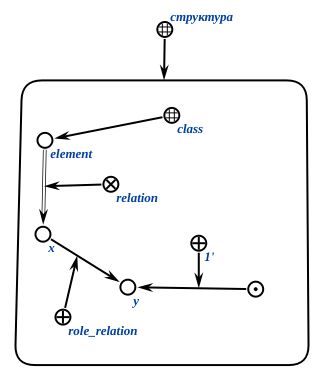
\includegraphics[scale=1]{author/part2/figures/chapter_kb/structure.png}
%	\caption{Представление структуры в SCg}
%	\label{fig:structure_scg}
%\end{figure}

Выделяют следующие классы структур:
\begin{SCn}
	\scnheader{структура}
	\begin{scnrelfromset}{разбиение}
	\scnitem{связная структура}
	\scnitem{несвязная структура}
\end{scnrelfromset}
	\begin{scnrelfromset}{разбиение}
	\scnitem{тривиальная структура}
	\scnitem{нетривиальная структура}
\end{scnrelfromset}
\end{SCn}

\textit{Структуре}, представленной в \textit{SC-коде}, поставим в соответствие орграф, вершинами которого являются \textit{sc-элементы}, а дугами – пары инцидентности, связывающие \textit{sc-коннекторы} с инцидентными им \textit{sc-элементами}, которые являются компонентами указанных \textit{sc-коннекторов}. Если полученный таким способом орграф является связным орграфом, то исходную структуру будем считать \textit{связной структурой}. Если полученный таким способом орграф не является связным орграфом, то исходную структуру будем считать \textit{несвязной структурой}.

Каждая выделяемая структура может выступать в роли либо тривиальной структуры: структуры, которая не содержит связки в качестве элементов, либо в роли нетривиальной структуры: структуры, среди элементов которой есть хотя бы одна связка.

Между структурами можно определять ряд соответствий, таких как гомоморфизм, полиморфизм, автоморфизм, изоморфизм, а также аналогичность структур, что позволяет фиксировать факт наличия некоторой аналогии, сходства и различия некоторых подструктур рассматриваемых структур.

%Пример отношения \textit{аналогичность структур} в SCg представлен на рисунке \textit{\nameref{fig:structure_analogy_scg}}.

%\begin{figure}[H]
%	\centering
%	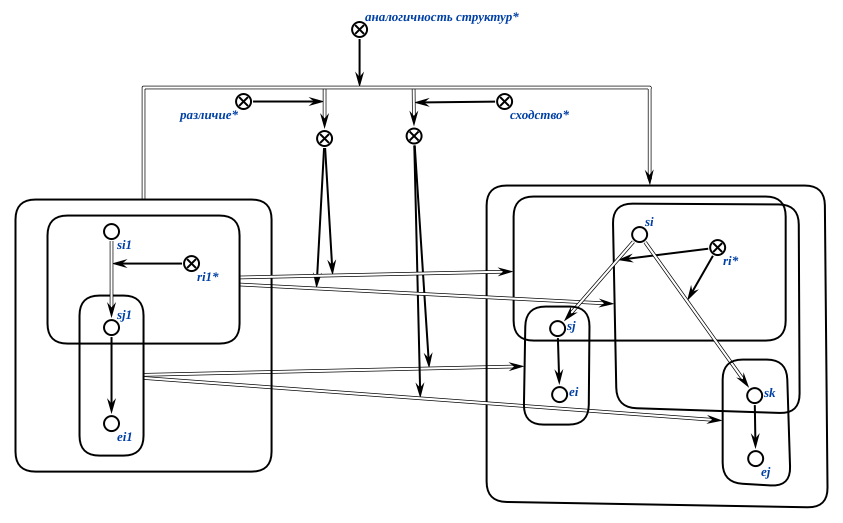
\includegraphics[scale=0.8]{author/part2/figures/chapter_kb/analogy.png}
%	\caption{Пример отношения аналогичность структур в SCg}
%	\label{fig:structure_analogy_scg}
%\end{figure}

\section{Формальная онтология семантических окрестностей}

Для спецификации отдельных сущностей в рамках базы знаний вводиться понятие \textit{семантической окрестности}. Семантическая окрестность представляет собой спецификацию (описание) заданной сущности, знак которой указывается как ключевой элемент этой спецификации.

Набор признаков, по которым можно специфицировать сущности, различен.

Различают полную и базовую семантические окрестности.

\begin{SCn}
	\scnheader{полная семантическая окрестность}
	\scnidtf{полная спецификация некоторой описываемой сущности}
\end{SCn}

Структура \textit{полной семантической окрестности} определяется прежде всего семантической типологией описываемой сущности.
Так, например, для понятия в \textit{полную семантическую окрестность} необходимо включить следующую
информацию (при наличии):
\begin{itemize}
	\item{варианты идентификации на различных внешних языках (sc-идентификаторы)};
	\item{принадлежность некоторой предметной области с указанием роли, выполняемой в рамках этой предметной области};
	\item{теоретико-множественные связи заданного понятия с другими sc-элементами};
	\item{определение или пояснение};
	\item{высказывания, описывающие свойства указанного понятия};
	\item{задачи и их классы, в которых данное понятие является ключевым};
	\item{описание типичного примера использования указанного понятия};
	\item{экземпляры описываемого понятия}.
\end{itemize}

Для понятия, являющегося отношением дополнительно указываются:
\begin{itemize}
	\item {домены};
	\item{область определения};
	\item{схема отношения};
	\item{классы отношений, которым принадлежит описываемое отношение}.
\end{itemize}

\begin{SCn}
	\scnheader{базовая семантическая окрестность}
	\scnidtf{минимально достаточная семантическая окрестность}
	\scnidtf{минимальная спецификация описываемой сущности}
\end{SCn}

Структура \textit{базовой семантической окрестности} определяется прежде всего семантической типологией описываемой сущности. Так, например, для понятия в \textit{базовую семантическую окрестность} необходимо включить следующую  информацию (при наличии):
\begin{itemize}
	\item {варианты идентификации на различных внешних языках (sc-идентификаторы)};
	\item {принадлежность некоторой предметной области с указанием роли, выполняемой в рамках этой предметной области};
	\item{определение или пояснение}.
\end{itemize}

Для понятия, являющегося отношением дополнительно указываются:
\begin{itemize}
	\item {домены};
	\item {область определения};
	\item {описание типичного примера связки указанного отношения (спецификация типичного экземпляра)}.
\end{itemize}

\section{Формальная онтология предметных областей}

Важнейшим этапом разработки баз знаний является процесс выделения описываемых предметных областей и их представления в базе знаний.

Понятие \textit{\textbf{предметной области}} является важнейшим методологическим приемом, позволяющим выделить из всего многообразия исследуемого Мира только определенный класс исследуемых сущностей и только определенное семейство отношений, заданных на указанном классе. То есть осуществляется локализация,
фокусирование внимания только на этом, абстрагируясь от всего остального исследуемого Мира.

Каждой \textit{предметной области} можно поставить в соответствие:
\begin{itemize}
	\item {семейство соответствующих ей онтологий разного вида};
	\item {множество семантических окрестностей, описывающих объекты исследования этой предметной области}.
\end{itemize}


\section{Формальная онтология онтологий}

Для формальной спецификации соответствующей предметной области,
ориентированной на описание свойств и взаимосвязей понятий, входящих в состав указанной предметной области, используется такой вид знаний, как \textit{онтология}.

\begin{SCn}
	\scnheader{онтология}
	\scnidtf{sc-онтология}
	\scnidtf{семантическая спецификация любого знания, имеющего достаточно сложную структуру, любого целостного
		фрагмента базы знаний – предметной области, метода решения сложных задач некоторого класса, описания
		истории некоторого вида деятельности, описания области выполнения некоторого множества действий
		(области решения задач), языка представления методов решения задач и т.д}
\end{SCn}

Онтология включает в себя:
\begin{itemize}
	\item {типологию специфицируемого знания};
	\item{связи специфицируемого знания с другими знаниями};
	\item{спецификацию ключевых понятий, используемых в специфицируемом знании, а также ключевых экземпляров некоторых таких понятий}.
\end{itemize}

Онтологии являются важнейшим видом знаний, обеспечивающих семантическую систематизацию знаний, хранимых в памяти интеллектуальных компьютерных систем (в т.ч. ostis-систем), и, соответственно, семантическую структуризацию баз знаний.

%\input{author/references}
\chapter{Смысловое представление логических формул и высказываний в различного вида логиках}
\chapauthortoc{Шункевич Д.~В.\\Василевская А.~П.\\Орлов М.~К.\\Ивашенко В.~П.}
\label{chapter_logic}

\begin{SCn}
	\begin{scnrelfromlist}{автор}
		\scnitem{Шункевич Д.~В.}
		\scnitem{Василевская А.~П.}
		\scnitem{Орлов М.~К.}
		\scnitem{Ивашенко В.~П.}
	\end{scnrelfromlist}
	
	\bigskip
	
	\scntext{аннотация}{В главе рассмотрено представление логических формул и высказываний как для классических логик и их приложений (прикладных логик), так и представление некоторых понятий неклассических логик.}
	
	\bigskip
	
	\begin{scnrelfromlist}{подраздел}
		\scnitem{\ref{sec_class_logic}~\nameref{sec_class_logic}}
		\scnitem{\ref{sec_applied_logic}~\nameref{sec_applied_logic}}
		\scnitem{\ref{sec_nonclass_logic}~\nameref{sec_nonclass_logic}}
	\end{scnrelfromlist}
	
	\bigskip
	
	\begin{scnrelfromlist}{ключевое понятие}
		\scnitem{логическая формула}
		\scnitem{атомарная логическая формула}
		\scnitem{неатомарная логическая формула}
		\scnitem{замкнутая логическая формула}
		\scnitem{открытая логическая формула}
		\scnitem{высказывание}
		\scnitem{атомарное высказывание}
		\scnitem{неатомарное высказывание}
		\scnitem{фактографическое высказывание}
		\scnitem{нефактографическое высказывание}
		\scnitem{атомарное фактографическое высказывание}
		\scnitem{атомарное нефактографическое высказывание}
		\scnitem{неатомарное нефактографическое высказывание}
		\scnitem{выполнимая логическая формула}
		\scnitem{невыполнимая логическая формула}
		\scnitem{общезначимая логическая формула}
		\scnitem{нейтральная логическая формула}				
		\scnitem{необщезначимая логическая формула}
		\scnitem{логическая формула, равнозначная логической константе}				
		\scnitem{атомарное существование}			
		\scnitem{кратность существования}			
		\scnitem{единственность существования}			
		\scnitem{иррефлексивное слотовое бинарное отношение}
		\scnitem{иррефлексивное неслотовое бинарное отношение}
		\scnitem{рефлексивное слотовое бинарное отношение}
		\scnitem{рефлексивное неслотовое бинарное отношение}
		\scnitem{транзитивное слотовое бинарное отношение}
		\scnitem{транзитивное неслотовое бинарное отношение}
		\scnitem{симметричное слотовое бинарное отношение}
		\scnitem{симметричное неслотовое бинарное отношение}
		\scnitem{антисимметричное слотовое бинарное отношение}
		\scnitem{антисимметричное неслотовое бинарное отношение}
		\scnitem{слотовое бинарное отношение}
		\scnitem{неслотовое бинарное отношение}
		\scnitem{слотовое отношение эквивалентности}
		\scnitem{неслотовое отношение эквивалентности}
		\scnitem{слотовое отношение нестрогого порядка}
		\scnitem{неслотовое отношение нестрогого порядка}
		\scnitem{секвенция}
		\scnitem{метаструктура}
		\scnitem{модальный оператор}
		\scnitem{модальное правило вывода}
		\scnitem{отношение становления структур}
		\scnitem{последовательность мышления}
		\scnitem{немонотонный вывод на конечном sc-множестве посылок}
		\scnitem{выводимое множество}
	\end{scnrelfromlist}
	
	\bigskip
	
	\begin{scnrelfromlist}{ключевое отношение}
		\scnitem{высказывание*}
		\scnitem{неразрешимое высказывание*}
		\scnitem{истинное высказывание*}
		\scnitem{ложное высказывание*}
		\scnitem{подформула*}				
		\scnitem{логическая связка*}				
		\scnitem{конъюнкция*}						
		\scnitem{дизъюнкция*}								
		\scnitem{отрицание*}
		\scnitem{строгая дизъюнкция*}	
		\scnitem{эквиваленция*}
		\scnitem{импликация*}
		\scnitem{если\scnrolesign}										
		\scnitem{то\scnrolesign}												
		\scnitem{квантор*}	
		\scnitem{всеобшность*}	
		\scnitem{существование*}	
		\scnitem{неатомарное существование*}
		\scnitem{нечеткая истинность*}
		\scnitem{конструктивно истинное высказывание*}
		\scnitem{верное высказывание*}
		\scnitem{монотонное бинарное отношение*}
		\scnitem{неискаженное высказывание*}
	\end{scnrelfromlist}

	\begin{scnrelfromlist}{ключевое знание}
		\scnitem{Описание понятия формальной теории}
		\scnitem{Описание понятия утверждения}				
		\scnitem{Описание понятия определение}
	\end{scnrelfromlist}
	
	\bigskip
	
	\begin{scnrelfromlist}{ключевой знак}
		\scnitem{Отношение выводимости}
		\scnitem{Отношение выводимости на конечных множествах}
		\scnitem{Отношение выводимости на конечных множествах полносвязно представленных множеств}
		\scnitem{Отношение выводимости на секвенциях}
	\end{scnrelfromlist}
	
	\bigskip
	
	\begin{scnrelfromlist}{библиографическая ссылка}		
		\scnitem{\scncite{Klini1973}}
		\scnitem{\scncite{Gribomon1990}}
		\scnitem{\scncite{Gribomon1998}}
		\scnitem{\scncite{Dragalin}}
		\scnitem{\scncite{Vagin2008}}
		\scnitem{\scncite{Golenkov2001b}}
		\scnitem{\scncite{Tarasov2007}}
		\scnitem{\scncite{Cintula2011}}		
		\scnitem{\scncite{Ivashenko2014diss}}
		\scnitem{\scncite{Ivashenko2017}}
		\scnitem{\scncite{Letichevskij2003}}
	\end{scnrelfromlist}
	
\end{SCn}

%Перенесено из chapter_logic_productions
%Язык SCL является логическим языком графового типа, используемым ostis-системами. Тексты языка SCL представляют собой однородные семантические сети, являющиеся текстами языка SC. Алфавит языка SCL отдельно не выделяется, так как используется алфавит SC-кода, на котором можно описать любые утверждения, явления, закономерности, программы и любые другие знания. Язык SCL позволяет записывать тексты языка логики высказываний, языка логики предикатов и любых других логических языков. SC-код является метаязыком как для языка SCL, так и для самого себя, то есть он позволяет описывать смысл формул, записанных на SCL. Многие формальные языки, в отличие от SC, недостаточно богаты, чтобы быть метаязыком для самих себя. 

%Одной из важных особенностей SCL является его способность представления текстов языка логики предикатов с учетом семантики этих текстов (высказываний). Язык SCL естественным образом ориентирован на работу в формальной системе языка логики предикатов. Язык SC позволяет записать любые отношения и соответствия в графовом представлении. Значению предиката от некоторого набора sc-переменных соответствует результат операции поиска по шаблону некоторой sc-конструкции (найдена или не найдена), в которую входят sc-константы и/или sc-переменные с соответствующей конфигурацией связей между ними. Подход, основанный на языке SCL для представления формул предоставляет возможность явно не записывать кванторы общности и существования (это не запрещается, однако является излишним). Квантор существования является "встроенным"{} понятием в том смысле, что если некоторый sc-элемент входит в некоторую sc-структуру, то соответствующее понятие существует в этой sc-структуре. Таким образом, квантор существования накладывается автоматически (если иной квантор не наложен явно) на те sc-переменные, которые входят в атомарные логические формулы. Квантор всеобщности накладывается по умолчанию (если иной квантор не наложен явно) на переменные, входящие в связки эквиваленции и импликации в соответствии с денотационной семантикой логических языков.

% Вагин дедукция и обобщения в системах принятия решений
\section{Смысловое представление логических формул и формальных теорий классической логики}
\label{sec_class_logic}
Появление \textit{формальных систем} было обусловлено осознанием того факта, что совершенно различные системы, будь то технические, социальные, экономические или биологические, обладают глубоким сходством. Действительно, каждая конкретная система состоит из каких-то первичных (базовых) элементов, обладающих какими-то свойствами. Затем, исходя из наличия исходных описаний, можно логическим путем вывести описание новых свойств, причем утверждения о наличии исходных или выведенных свойств воспринимаются как истинные на основании смысла определений данных элементов.

\scnkeyword{формальная теория} --- это \textit{множество} \textit{высказываний}, которые считаются истинными в рамках данной \scnkeyword{формальной теории}.

Аксиоматические системы --- это системы с наличием определенного числа исходных заранее выбранных и фиксированных высказываний, называемых аксиомами.

\textit{высказывания} могут быть как фактографическими, так и нефактографическими. Некоторые \textit{высказывания} считаются аксиомами, а другие доказываются на основе других высказываний в рамках этой же \scnkeyword{формальной теории}.

Каждая формальная теория интерпретируется (то есть ее \textit{высказывания} являются истинными) на какой-либо \textit{предметной области}, которая является максимальным из \textit{фактографических высказываний} (их \textit{объединением*}),  входящих в состав этой \scnkeyword{формальной теории}.

Каждой \scnkeyword{формальной теории} соответствует одна \textit{предметная область}, которая входит в нее под атрибутом \textit{предметная область\scnrolesign}.

Каждая \textit{формальная теория} может рассматриваться как \textit{конъюнктивное высказывание}, априори истинное (с чьей-то точки зрения) при интерпретации на соответствующей предметной области.

Каждая \textit{формальная теория} задается \textit{алфавитом}, \textit{формулами}, \textit{аксиомами}, \textit{правилами вывода}.

%\scnrelfrom{источник}{\scncite{Serhievskaya2004}}

\textit{предметная область} является \textit{максимальным фактографическим высказыванием} \textit{формальной теории}, которая интерпретируется на данной \textit{предметной области}.

\textbf{\textit{аксиома}} --- это \textit{высказывание}, истинность которого не требует доказательства в рамках рассматриваемой \textit{формальной теории}.

\textbf{\textit{теорема}} --- это \textit{высказывание}, истинность которого доказывается в рамках рассматриваемой \textit{формальной теории}.

\begin{SCn}
\scnheader{логическая формула}
\begin{scnrelfromset}{разбиение}
	\scnitem{атомарная логическая формула}
	\scnitem{неатомарная логическая формула}
\end{scnrelfromset}
\begin{scnrelfromset}{разбиение}
	\scnitem{замкнутая логическая формула}
	\scnitem{открытая логическая формула}
\end{scnrelfromset}
\end{SCn}
\begin{SCn}
\scnheader{высказывание}
\scnsubset{логическая формула}
\begin{scnrelfromset}{разбиение}
	\scnitem{атомарное высказывание}
	\scnitem{неатомарное высказывание}
\end{scnrelfromset}
\begin{scnrelfromset}{разбиение}
	\scnitem{фактографическое высказывание}
	\begin{scnindent}
		\scnsubset{замкнутая логическая формула}
	\end{scnindent}
	\scnitem{нефактографическое высказывание}
\end{scnrelfromset}
\end{SCn}

Под \textbf{\textit{высказыванием}} понимается некоторая \textit{структура} (в которую входят \textit{sc-константы} из некоторой предметной области и/или \textit{sc-переменные}) или \textit{логическая связка}, которая может трактоваться как истинная или ложная в рамках какой-либо \textit{предметной области}.

Истинность \textbf{\textit{высказывания}} задается путем указания принадлежности знака этого высказывания \textit{формальной теории}, соответствующей данной \textit{предметной области}. Ложность высказывания задается путем указания принадлежности знака \textit{отрицания*} этого высказывания данной \textit{формальной теории}.

Явно указанная непринадлежность \textbf{\textit{высказывания}} \textit{формальной теории} может говорить как о его ложности в рамках данной теории (если это указано рассмотренным выше образом), так и о том, что данное  \textbf{\textit{высказывание}} вообще не рассматривается в данной \textit{формальной теории} (например, использует понятия, не принадлежащие данной \textit{предметной области}).

Одно и то же \textbf{\textit{высказывание}} может быть истинно в рамках одной \textit{формальной теории} и ложно в рамках другой.

%\begin{SCn}
%% Добавить темпоральное высказывание
%\scnheader{высказывание формальной теории\scnrolesign}
%\begin{scnrelfromset}{разбиение}
%	\scnitem{истинное высказывание\scnrolesign}
%	\scnitem{ложное высказывание\scnrolesign}
%%	\scnitem{нечеткое высказывание\scnrolesign}
%	\scnitem{бессмысленное высказывание\scnrolesign}
%\end{scnrelfromset}
%\end{SCn}

%\textbf{\textit{истинное высказывание}} --- высказывание, знак которого принадлежит изучаемой формальной теории.
%Нечеткое высказывание --- высказывание, возможно истинное или ложное в рамках изучаемой формальной теории (высказывание, возможно истинное или ложное в рамках данной формальной теории).
%\textbf{\textit{бессмысленное высказывание}} --- высказывание, не рассматриваемое в рамках данной формальной теории. Высказывание является бессмысленным в рамках заданной формальной теории, если в какое-либо \textit{атомарное высказывание} в его составе (или в само это высказывание, если оно является атомарным) входит какая-либо \textit{sc-константа}, не являющаяся элементом предметной области, описываемой указанной \textit{формальной теорией}.

\begin{SCn}
\scnheader{атомарное высказывание}
\scnsubset{структура}
\begin{scnrelfromset}{разбиение}
	\scnitem{атомарное фактографическое высказывание}
	\scnitem{атомарное нефактографическое высказывание}
\end{scnrelfromset}
\end{SCn}

\textbf{\textit{атомарное высказывание}} --- это \textit{высказывание}, которое не является \textit{неатомарным высказыванием}.

\textbf{\textit{неатомарное высказывание}} --- это \textit{высказывание}, в состав которого входят только знаки \textit{логических формул} или множества связываемых переменных. Следует отметить, что невозможно говорить об истинности либо ложности \textbf{\textit{неатомарного высказывания}} в рамках какой-либо \textit{формальной теории}, в случае, когда невозможно установить истинность либо ложность любого из его элементов в рамках этой же \textit{формальной теории} или интерпретации этих элементов.

Под \textit{фактографическим высказыванием} понимается:
\begin{textitemize}
	\item \textit{атомарное высказывание}, в состав которого не входит ни одна \textit{sc-переменная};
	\item \textit{неатомарное высказывание}, все элементы которого также являются \textbf{\textit{фактографическими высказываниями}}.
\end{textitemize}

\begin{SCn}
\scnheader{высказывание*}
\scnidtf{бинарное ориентированное отношение, каждая \textit{пара} которого связывает (1) знак некоторой \textit{предметной области} и (2) знак некоторого \textit{высказывания}.}
\begin{scnrelfromset}{разбиение}
	\scnitem{ложное высказывание*}
	\scnitem{неразрешимое высказывание*}
%	\begin{scnindent}
%			\scnsuperset{гипотеза}
%	\end{scnindent}}
	\scnitem{истинное высказывание*}	
\end{scnrelfromset}
\end{SCn}

%\scntext{предъявляемое требование}{Все \textit{sc-элементы}, входящие в состав \textit{предметной области}, описываемой высказыванием, (включая и \textit{sc-переменные}, которые, хоть и редко, но могут входить в состав некоторых \textit{предметных областей}) 
%\textit{sc-элементами} для всех высказываний, соответствующих этой \textit{предметной области}.}

\scntext{предъявляемое требование}{Все \textit{sc-константы}, входящие в состав всех \textit{атомарных логических формул}, входящих в состав всех \textit{высказываний}, описывающих некоторую \textit{предметную область} должны входить в состав описываемой \textit{предметной области}.}

\begin{SCn}
\scnheader{следует отличать*}
\begin{scnhaselementset}
	\scnitem{высказывание*}
	\begin{scnindent}
		\scniselement{бинарное ориентированное отношение}
		\scnidtf{быть высказыванием, описывающим заданную предметную область*}
		\begin{scnindent}
			\scntext{сокращение}{быть высказыванием*}
		\end{scnindent}
	\end{scnindent}
	\scnitem{высказывание}
	\begin{scnindent}
		\scnsubset{логическая формула}
		\scnidtf{Второй домен отношения ``быть высказыванием''}
	\end{scnindent}
\end{scnhaselementset}
\end{SCn}

\begin{SCn}
\scnheader{нефактографическое высказывание}
\begin{scnrelfromset}{разбиение}
	\scnitem{атомарное нефактографическое высказывание}
	\scnitem{неатомарное нефактографическое высказывание}
\end{scnrelfromset}
\end{SCn}

Под \textit{нефактографическим высказыванием} понимается:
\begin{textitemize}
	\item \textit{атомарное нефактографическое высказывание}, в состав которого входит хотя бы одна \textit{sc-переменная};
	\item \textit{неатомарное нефактографическое высказывание}, хотя бы один элемент которого является \textbf{\textit{нефактографическим высказыванием}}.
\end{textitemize}

Под \textbf{\textit{атомарным нефактографическим высказыванием}} понимается \textit{атомарное высказывание}, которое является \textit{нефактографическим высказыванием}.

\textbf{\textit{атомарное нефактографическое высказывание}} --- это \textit{нефактографическое высказывание}, которая не является \textit{неатомарным нефактографическим высказыванием}.

\textbf{\textit{атомарная логическая формула}} --- это \textit{логическая формула}, которая не является \textit{неатомарной логической формулой}.

По умолчанию \textbf{\textit{атомарное нефактографическое высказывание}} трактуется как \textit{высказывание} о существовании, то есть наличия в памяти значений, соответствующих всем \textit{sc-переменным}, входящим в состав данной формулы и не попадающих под действие какого-либо другого \textit{квантора} (указанного явно или по умолчанию). Таким образом, на все \textit{sc-переменные}, входящие в состав \textit{атомарного нефактографического высказывания} и не попадающие под действие какого-либо другого \textit{квантора}, неявно накладывается квантор \textit{существования*}.

\begin{SCn}
\scnheader{логическая формула}
\begin{scnrelfromset}{разбиение}
	\scnitem{выполнимая логическая формула}
	\begin{scnindent}
		\begin{scnrelfromset}{разбиение}
			\scnitem{общезначимая логическая формула}
			\scnitem{нейтральная логическая формула}
		\end{scnrelfromset}
	\end{scnindent}
	\scnitem{невыполнимая логическая формула}
\end{scnrelfromset}
\end{SCn}

Под \textbf{\textit{неатомарным нефактографическим высказыванием}} понимается \textit{неатомарное высказывание}, которое является \textit{нефактографическим высказыванием}.

Для того, чтобы рассмотреть типологию \textbf{\textit{неатомарных логических формул}}, будем говорить, что исследуется истинность самой \textbf{\textit{неатомарной логической формулы}} и всех ее \textit{подформул*} в рамках одной и той же \textit{формальной теории}, при этом не важно, какой именно. Также считается, что в рассматриваемой \textit{формальной теории} каждая \textit{подформула*} рассматриваемой \textbf{\textit{неатомарной логической формулы}} в рамках этой \textit{формальной теории} может однозначно трактоваться как либо истинная, либо ложная. В противном случае мы не можем говорить об истинности либо ложности исходной \textbf{\textit{неатомарной логической формулы}} в рамках этой \textit{формальной теории}.

Будем называть \textbf{\textit{подформулой*}} \textit{неатомарной логической формулы} \textbf{\textit{fi}} любую \textit{логическую формулу} \textbf{\textit{fj}}, являющуюся элементом исходной формулы \textbf{\textit{fi}}, а также любую \textbf{\textit{подформулу*}} формулы \textbf{\textit{fj}}.

\begin{SCn}
\scnheader{подформула*}
\scnidtf{частная формула*}
\scniselement{бинарное отношение}
\scniselement{ориентированное отношение}
\scniselement{транзитивное отношение}
%\scnrelfrom{описание примера}{\scnfileitem{figures/sd_logical_formulas/subformula.png}}
\end{SCn}

\begin{figure}[H]
	\caption{Формализация примера подформулы}
	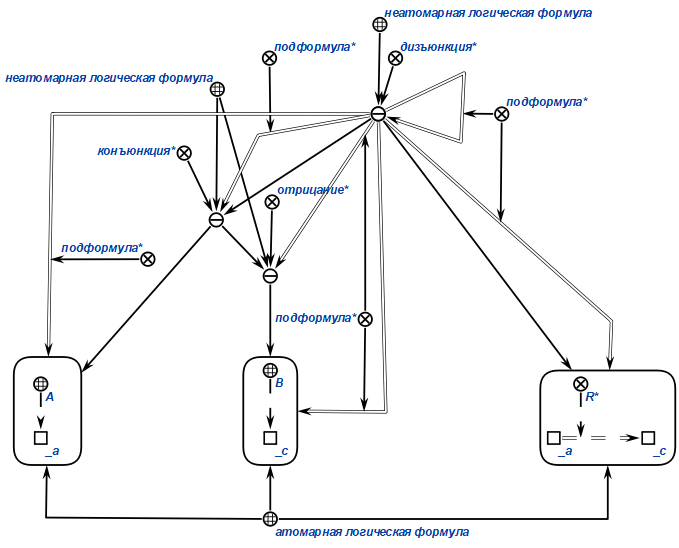
\includegraphics[scale=0.8]{author/part2/figures/logic/subformula.png}
	\label{fig:modus_ponens}
\end{figure}

\textbf{\textit{утверждение}} --- это \textit{семантическая окрестность} некоторой \textit{логической формулы}, в которую входит полный текст этой \textit{логической формулы}, а также факт принадлежности этой \textit{логической формулы} некоторой \textit{формальной теории}.

Знак \textit{логической формулы}, семантическая окрестность которой представляет собой утверждение, является \textit{главным ключевым sc-элементом\scnrolesign} в рамках этого \textbf{\textit{утверждения}}. Знаки понятий соответствующей \textit{предметной области}, которые входят в состав какой-либо \textit{подформулы*} указанной \textit{логической формулы}, будут \textit{ключевыми sc-элементами\scnrolesign} в рамках этого \textbf{\textit{утверждения}}.
	
Полный текст некоторой \textit{логической формулы} включает в себя:
\begin{textitemize}
	\item{знак самой этой \textit{логической формулы}};
	\item{знаки всех ее \textit{подформул*}};
	\item{элементы всех \textit{логических формул}, знаки которых попали в данную структуру;}
	\item{все пары принадлежности, связывающие \textit{логические формулы}, знаки которых попали в данную структуру, с их компонентами.}
\end{textitemize}

Таким образом, факт принадлежности (истинности) логической формулы нескольким \textit{формальным теориям} будет порождать новое утверждение для каждой такой \textit{формальной теории}. Текст \textbf{\textit{утверждения}} входит в состав \textit{логической онтологии}, соответствующей \textit{предметной области}, на которой интерпретируется \textit{главный ключевой sc-элемент\scnrolesign} данного утверждения.

Правило идентификации экземпляров \textbf{\textit{утверждения}} в рамках \textit{Русского языка} именуются по следующим правилам:
\begin{textitemize}
	\item{в начале идентификатора пишется сокращение \textbf{Утв.};}
	\item{далее в круглых скобках через точку с запятой перечисляются основные идентификаторы \textit{ключевых \mbox{sc-элементов}\scnrolesign} данного \textbf{\textit{утверждения}}. Порядок определяется в каждом конкретном случае в зависимости от того, свойства каких из этих \textit{понятий} описывает данное \textbf{\textit{утверждение}} в большей или меньшей степени.}
\end{textitemize}

%\scntext{описание примера}{\textit{Утв. (параллельность*; секущая*)}}
Могут быть исключения для \textbf{\textit{утверждений}}, названия которых закрепились исторически, например, \textit{Теорема Пифагора}, \textit{Аксиома о прямой и точке}.


%\scnrelfrom{описание примера}{\scnfilescg{figures/sd_logical_formulas/statement.png}}
%Утверждение показывает, что соответствующие углы при пересечении параллельных прямых секущей равны.

\textbf{\textit{определение}} --- это \textit{утверждение}, \textit{главным ключевым sc-элементом\scnrolesign} которого является связка \textit{эквиваленции*}, однозначно определяющая некоторое понятие на основе других понятий.

Каждое определение имеет ровно один \textit{ключевой sc-элемент\scnrolesign} (не считая \textit{главного ключевого sc-элемента\scnrolesign}).

Для одного и того же понятия в рамках одной \textit{формальной теории} может существовать несколько \textit{утверждений об эквиваленции*}, однозначно задающих некоторое понятие на основе других, однако только одно такое \textit{утверждение} в рамках этой \textit{формальной теории} может быть отмечено как \textbf{\textit{определение}}. Остальные \textit{утверждения об эквиваленции*} могут трактоваться как \textit{пояснения} данного понятия.

Правило идентификации экземпляров \textbf{\textit{определения}} в рамках \textit{Русского языка} именуются по следующим правилам:
\begin{textitemize}
	\item{в начале идентификатора пишется сокращение \textbf{Опр.};}
	\item{далее в круглых скобках через точку с запятой записывается основной идентификатор  \textit{ключевого sc-элемента\scnrolesign} данного \textbf{\textit{определения}}.}
\end{textitemize}


%\scntext{описание примера}{\textit{Опр. (ромб)}}
%\scnrelfrom{описание примера}{\scnfilescg{figures/sd_logical_formulas/definition.png}}
%\scnnote{Определение показывает, что ромб — это четырехугольник, у которого все стороны равны.}
\begin{SCn}
\scnheader{общезначимая логическая формула}
\scnidtf{тождественно истинная логическая формула}
\scnsubset{выполнимая логическая формула}
\scnsubset{логическая формула, равнозначная логической константе}
\end{SCn}
% Вагин, дедукция и обобщение в системах принятия решений
\textbf{\textit{общезначимая логическая формула}} --- это \textit{логическая формула}, для которой не существует \textit{формальной теории}, в рамках которой она была бы ложной (или имела бы ложную интерпретацию) с учетом истинности и ложности всех ее \textit{подформул*} (или их интерпретаций) в рамках этой же \textit{формальной теории}.

\begin{figure}[H]
\caption{Формализация закона тождества}
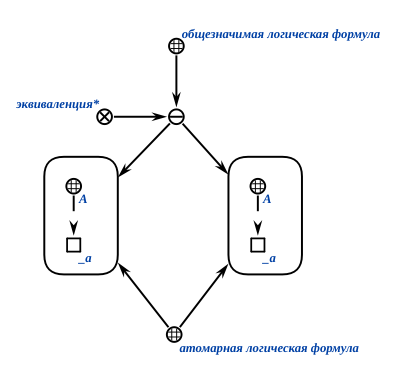
\includegraphics[scale=0.8]{author/part2/figures/logic/valid_formula.png}
\label{fig:valid_formula}
\end{figure}

\begin{SCn}
\scnheader{противоречивая логическая формула}
\scnidtf{тождественно ложная логическая формула}
\scnsubset{невыполнимая логическая формула}
\scnsubset{логическая формула, равнозначная логической константе}
\end{SCn}
% Вагин, дедукция и обобщение в системах принятия решений
\textbf{\textit{противоречивая логическая формула}} --- это \textit{логическая формула}, для которой не существует \textit{формальной теории}, в рамках которой она была бы истинной (или имела бы истинную интерпретацию) с учетом истинности и ложности всех ее \textit{подформул*} (или их интерпретаций) в рамках этой же \textit{формальной теории}.

\begin{figure}[H]
	\caption{Формализация закона противоречия}
	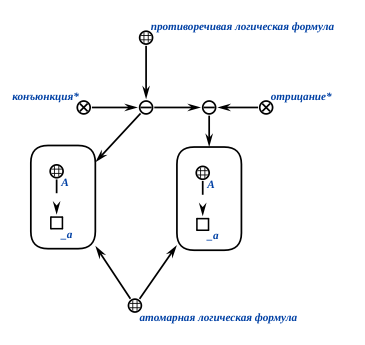
\includegraphics[scale=0.8]{author/part2/figures/logic/contradiction_formula.png}
	\label{fig:contradiction_formula}
\end{figure}

\begin{SCn}
\scnheader{нейтральная логическая формула}
\scnsubset{выполнимая логическая формула}
\end{SCn}

\textbf{\textit{нейтральная логическая формула}} --- это \textit{логическая формула}, для которой существует хотя бы одна \textit{формальная теория}, в рамках которой эта формула ложна (или имеет ложную интерпретацию), и хотя бы одна \textit{формальная теория}, в рамках которой эта формула истинна (или имеет ложную интерпретацию).

\begin{figure}[H]
	\caption{Формализация нейтральной логической формулы}
	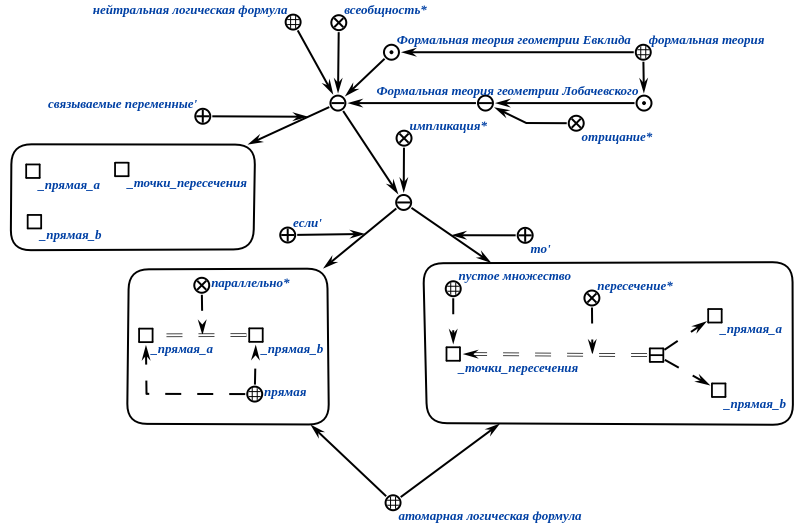
\includegraphics[scale=0.8]{author/part2/figures/logic/neutral_formula.png}
	\label{fig:neutral_formula}
\end{figure}

В \textit{Геометрии Евклида} в плоскости через точку, не лежащую на данной прямой, можно провести одну и только одну прямую, параллельную данной. В \textit{Геометрии Лобачевского} данный постулат является ложным.
В \textit{Сферической геометрии} все прямые пересекаются.

\begin{SCn}
\scnheader{непротиворечивая логическая формула}
\scnidtf{выполнимая логическая формула}
\begin{scnreltoset}{объединение}
	\scnitem{нейтральная логическая формула}
	\scnitem{общезначимая логическая формула}
\end{scnreltoset}
\end{SCn}

\textbf{\textit{непротиворечивая логическая формула}} --- это \textit{логическая формула}, для которой существует хотя бы одна \textit{формальная теория}, в рамках которой эта формула истинна (или имеет истинную интерпретацию).

\begin{SCn}
\scnheader{необщезначимая логическая формула}
%\scnidtf{невыполнимая логическая формула}
\begin{scnreltoset}{объединение}
	\scnitem{нейтральная логическая формула}
	\scnitem{противоречивая логическая формула}
\end{scnreltoset}
\end{SCn}

\textbf{\textit{необщезначимая логическая формула}} --- это \textit{логическая формула}, для которой существует хотя бы одна \textit{формальная теория}, в рамках которой эта формула ложна (или имеет ложную интерпретацию).

\textbf{\textit{логическая формула, равнозначная логической константе}} --- это \textit{логическая формула}, которая является либо только истинной (имеет только истинные интерпретации), либо только ложной (имеет только ложные интерпретации) в рамках всех \textit{формальных теорий}, в которых можно установить ее истинность или ложность.
\textbf{\textit{логическая формула, равнозначная логической константе}} --- это такая \textit{логическая формула}, которая является либо \textit{общезначимой логической формулой}, либо \textit{противоречивой логической формулой}.

\begin{SCn}
\scnheader{логическая связка*}
\scnidtf{неатомарная логическая формула}
\scnidtf{логический оператор*}
\scnidtf{пропозициональная связка*}
\scniselement{класс связок разной мощности}
\scnrelto{семейство подмножеств}{неатомарное высказывание}
\end{SCn}

\textbf{\textit{логическая связка*}} --- это отношение (класс связок), связками которого являются \textit{высказывания}, а областью определения которого является множество \textit{высказываний}, при этом само это отношение и некоторые его подмножества могут быть \textit{классами связок разной мощности}.

\begin{SCn}
\scnheader{конъюнкция*}
\scnidtf{логическое и*}
\scnidtf{логическое умножение*}
\scnsubset{логическая связка*}
\scniselement{неориентированное отношение}
\scniselement{класс связок разной мощности}
\scniselement{неунарное отношение}
\scnrelfrom{область определения}{логическая формула}
\end{SCn}

\textbf{\textit{конъюнкция*}} --- это множество конъюнктивных \textit{логических формул}, каждая из которых истинна (имеет истинные интерпретации) в рамках некоторой \textit{формальной теории} только в том случае, когда все ее компоненты истинны (имеют только соответствующие истинные интерпретации) в рамках этой же \textit{формальной теории}. 
%\textit{конъюнкция*} атомарных формул может быть представлена атомарной формулой, полученной путем объединения исходных атомарных формул.

\begin{figure}[H]
	\caption{Формализация примера конъюнкции}
	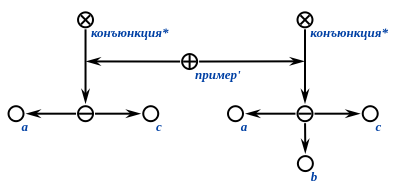
\includegraphics[scale=0.8]{author/part2/figures/logic/conjunction.png}
	\label{fig:conjunction}
\end{figure}

%logically incorrect figure
%\begin{figure}[H]
%	\caption{Формализация примера конъюнкции в геометрии}
%	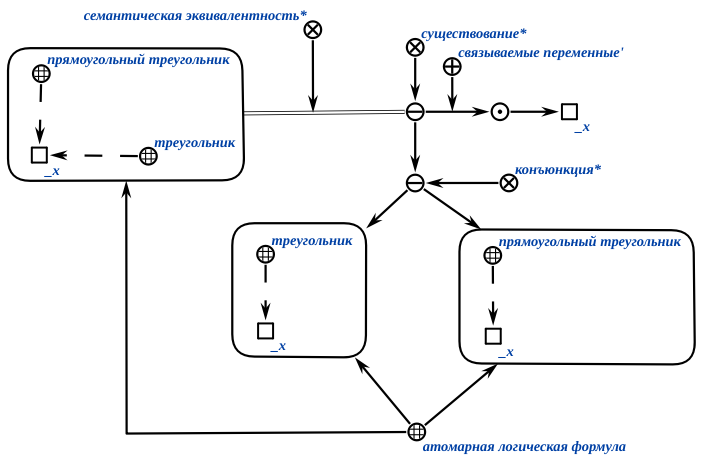
\includegraphics[scale=0.8]{author/part2/figures/logic/conjunction_triangles.png}
%	\label{fig:conjunction_triangles}
%	\scnexplanation{Данные конструкции эквивалентны по принципу $\exists x T(x) \land \exists x PT(x) \ \Longrightarrow \ \exists x (T(x) \land PT(x))$}
%\end{figure}

\begin{SCn}
\scnheader{дизъюнкция*}
\scnidtf{логическое или*}
\scnidtf{логическое сложение*}
\scnidtf{включающее или*}
\scnsubset{логическая связка*}
\scniselement{неориентированное отношение}
\scniselement{класс связок разной мощности}
\scniselement{неунарное отношение}
\scnrelfrom{область определения}{логическая формула}
\end{SCn}

\textbf{\textit{дизъюнкция*}} --- это множество дизъюнктивных \textit{логических формул}, каждая из которых истинна (имеет истинные интерпретации) в рамках некоторой \textit{формальной теории} только в том случае, когда хотя бы один его компонент является истинным (имеет соответствующую истинную интерпретацию) в рамках этой же \textit{формальной теории}.

Следует отметить, что каждая конъюнктивная и дизъюнктивная формула представляют собой связку (множество) своих непосредственных подформул, причем эти множества могут быть равными, однако, такие множества будем полагать различными, так как одно множество будет представлять конъюнкцию, а другое -- дизъюнкцию. Наличие равных, но различных множеств не допускается в классической математике, которая основывается, в том числе, на абстракции обобщения (все равные множества (абстракции) -- тождественны). Однако, такие множества могут существовать в неклассических математических моделях. Таким образом, в рамках языка SC будем использовать неклассическую математическую модель для представления логических формул классической математической логики.

\begin{figure}[H]
	\caption{Формализация примера дизъюнкции}
	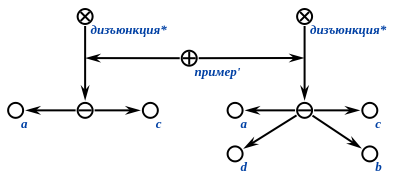
\includegraphics[scale=0.8]{author/part2/figures/logic/disjunction.png}
	\label{fig:disjunction}
\end{figure}

\begin{SCn}
\scnheader{отрицание*}
\scnsubset{логическая связка*}
\scnsubset{синглетон}
\scniselement{унарное отношение}
\scnrelfrom{область определения}{логическая формула}
\end{SCn}

\textbf{\textit{отрицание*}} --- это множество \textit{логических формул} об отрицании, каждое из которых истинно (имеет истинную интерпретацию) в рамках некоторой \textit{формальной теории} только в том случае, когда его единственный элемент является ложным (имеет ложную эту же интерпретацию) в рамках этой же \textit{формальной теории}.

\begin{figure}[H]
	\caption{Формализация примера отрицания}
	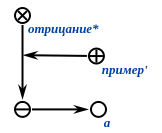
\includegraphics[scale=0.8]{author/part2/figures/logic/negation.png}
	\label{fig:negation}
\end{figure}

\begin{SCn}
\scnheader{строгая дизъюнкция*}
%\scnidtf{сложение по модулю 2*}
\scnidtf{исключающее или*}
\scnidtf{альтернатива*}
\scnsubset{логическая связка*}
\scniselement{неориентированное отношение}
\scniselement{класс связок разной мощности}
\end{SCn}

\textbf{\textit{строгая дизъюнкция*}} --- это множество строго дизъюнктивных \textit{логических формул}, каждое из которых истинно в рамках некоторой \textit{формальной теории} только в том случае, когда ровно один его компонент является истинным (имеет соответствующую истинную интерпретацию) в рамках этой же \textit{формальной теории}.

\begin{figure}[H]
	\caption{Формализация примера строгой дизъюнкции в геометрии}
	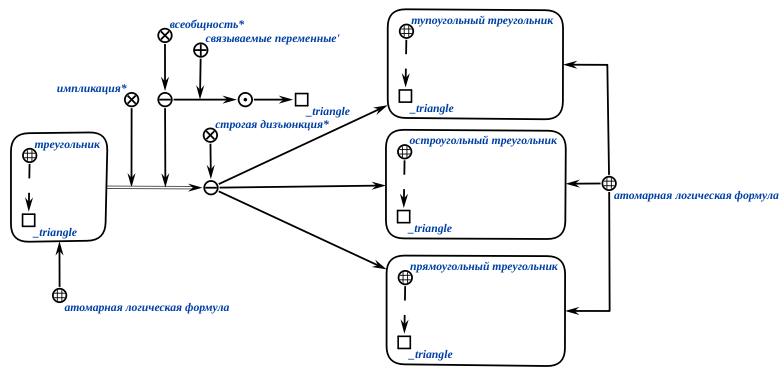
\includegraphics[scale=0.8]{author/part2/figures/logic/strict_disjunction_triangle.png}
	\label{fig:strict_disjunction_triangle}
\end{figure}
	\scnexplanation{Данная неатомарная логическая формула содержит следующую информацию: для любых переменных \_triangle если \_triangle является треугольником, то \_triangle является или тупоугольным треугольником, или остроугольным треугольником, или прямоугольным треугольником.}

\begin{figure}[H]
	\caption{Формализация примера строгой дизъюнкции}
	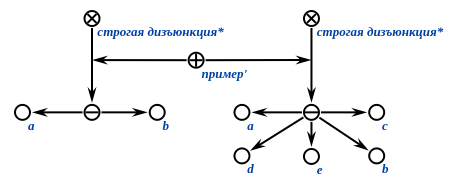
\includegraphics[scale=0.8]{author/part2/figures/logic/strictDisjunction.png}
	\label{fig:strict_disjunction}
\end{figure}

\textbf{\textit{строгая дизъюнкция*}} может быть представлена как \textit{дизъюнкция} \textit{конъюнкции} \textit{отрицания} первой логической формулы и второй логической формулы и \textit{конъюнкции} первой логической формулы и \textit{отрицания} второй логической формулы. Также она может быть представлена и в виде \textit{конъюнкции} \textit{дизъюнкций} двух логических формул и их \textit{отрицаний}.

\begin{figure}[H]
	\caption{Формализация примера строгой дизъюнкции}
	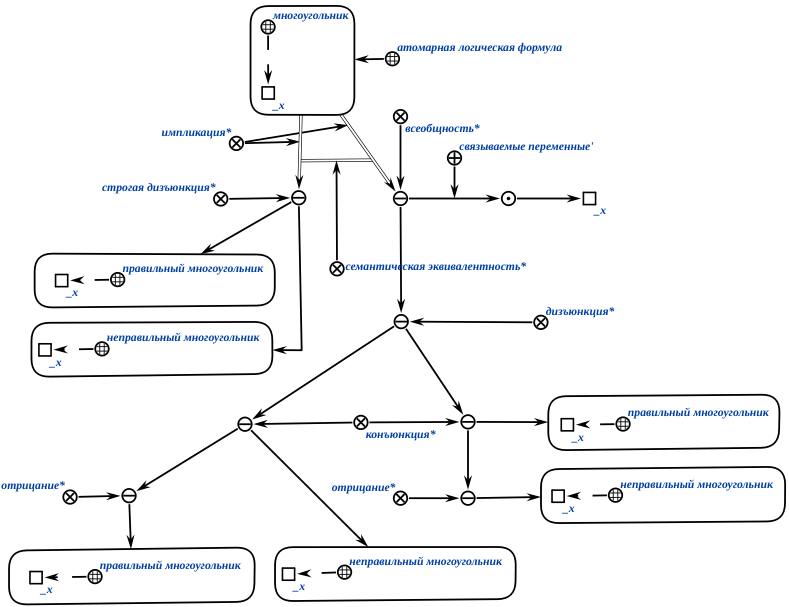
\includegraphics[scale=0.8]{author/part2/figures/logic/strict_disjunction_representation.png}
	\label{fig:strict_disjunction_representation}
\end{figure}

\begin{SCn}
\scnheader{импликация*}
\scnidtf{логическое следование*}
\scnsubset{логическая связка*}
\scniselement{бинарное отношение}
\scniselement{ориентированное отношение}
\scnrelfrom{область определения}{логическая формула}
\end{SCn}

\textbf{\textit{импликация*}} --- это множество импликативных \textit{логических формул}, каждая из которых состоит из посылки (первый компонент \textit{высказывания}) и следствия (второй компонент \textit{высказывания}).

Каждое импликативное \textit{высказывание} ложно в рамках некоторой \textit{формальной теории} в том случае, когда его посылка истинна, а заключение ложно в рамках этой же \textit{формальной теории}. В других случаях такое \textit{высказывание} истинно.

По умолчанию на все переменные, входящие в обе части высказывания об \textbf{\textit{импликации*}} (или хотя бы одну из \textit{подформул*} каждой части) неявно накладывается квантор \textit{всеобщности*}, при условии, что эти переменные не связаны другим \textit{квантором}, указанным явно.

\begin{figure}[H]
\caption{Формализация примера импликации}
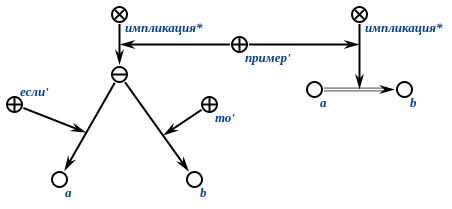
\includegraphics[scale=0.8]{author/part2/figures/logic/implication.png}
\label{fig:implication}
\end{figure}

\textbf{\textit{импликация*}} может быть представлена как \textit{дизъюнкция} \textit{отрицания} первой логической формулы и второй логической формулы или же как \textit{отрицание} \textit{конъюнкции} первой логической формулы и \textit{отрицания} второй логической формулы.

\begin{figure}[H]
	\caption{Формализация примера импликации}
	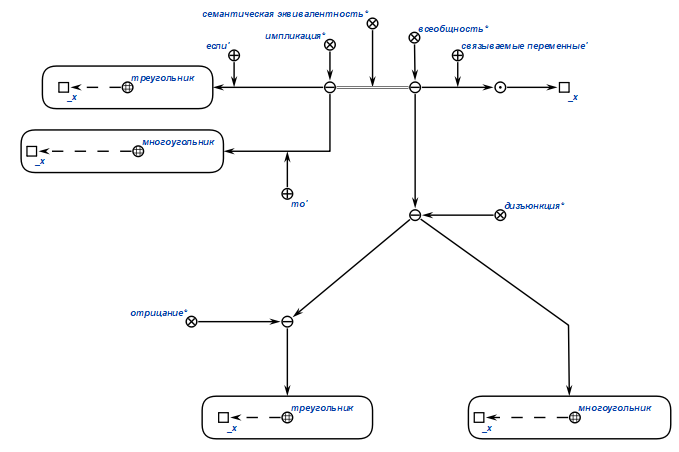
\includegraphics[scale=0.8]{author/part2/figures/logic/implication_representation.png}
	\label{fig:implication_representation}
\end{figure}

\begin{figure}[H]
	\caption{Формализация примера импликации}
	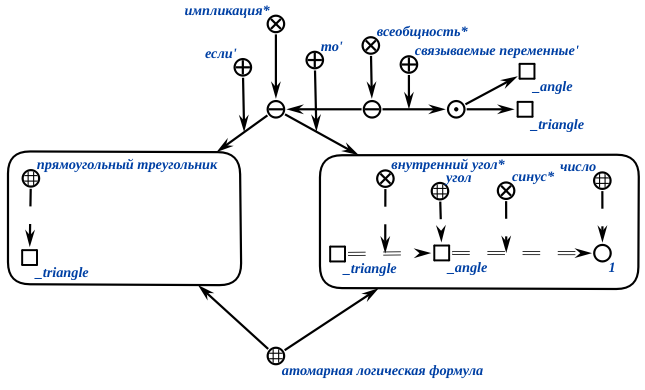
\includegraphics[scale=0.8]{author/part2/figures/logic/implication_triangle.png}
	\label{fig:implication_triangle}
\end{figure}
\vspace{-2\baselineskip}
\scnexplanation{Данная неатомарная логическая формула содержит следующую информацию: для любых переменных \_triangle и \_angle если \_triangle является прямоугольным треугольником, то синус его внутреннего угла \_angle равен единице.}

\begin{SCn}
\scnheader{если\scnrolesign}
\scnidtf{посылка\scnrolesign}
\scnsubset{1\scnrolesign}
\scniselement{ролевое отношение}
\end{SCn}

\textbf{\textit{если\scnrolesign}} --- это \textit{ролевое отношение}, используемое в связках \textit{импликации*} для указания посылки.

\begin{SCn}
\scnheader{то\scnrolesign}
\scnidtf{следствие\scnrolesign}
\scnsubset{2\scnrolesign}
\scniselement{ролевое отношение}
\end{SCn}

\textbf{\textit{то\scnrolesign}} --- это \textit{ролевое отношение}, используемое в связках \textit{импликации*} для указания следствия.

\begin{SCn}
\scnheader{эквиваленция*}
\scnidtf{эквивалентность*}
\scnsubset{логическая связка*}
\scniselement{бинарное отношение}
\scniselement{неориентированное отношение}
\scnrelfrom{область определения}{логическая формула}
\end{SCn}

\textbf{\textit{эквиваленция*}} --- это множество \textit{логических формул} об эквивалентности, каждое из которых истинно (имеет истинную интерпретацию) в рамках некоторой \textit{формальной теории} только в тех случаях, когда оба его компонента одновременно либо истинны (имеют соответствующие истинные интерпретации) в рамках этой же \textit{формальной теории}, либо ложны (имеют соответствующие ложные интерпретации).

По умолчанию на все переменные, входящие в обе части высказывания об \textbf{\textit{эквиваленции*}} (или хотя бы одну из \textit{подформул*} каждой части) неявно накладывается квантор \textit{всеобщности*}, при условии, что эти переменные не связаны другим \textit{квантором}, указанным явно.

\begin{figure}[H]
	\caption{Формализация примера эквиваленции}
	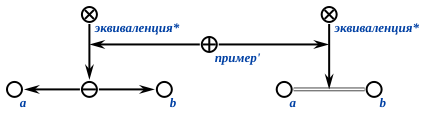
\includegraphics[scale=0.8]{author/part2/figures/logic/equivalent.png}
	\label{fig:equivalent}
\end{figure}

\textbf{\textit{эквиваленция*}} двух логических формул может быть представлена как \textit{дизъюнкция} \textit{конъюнкции} этих двух логических формул и \textit{конъюнкции} \textit{отрицаний} этих двух логических формул.

\begin{figure}[H]
	\caption{Формализация примера эквиваленции}
	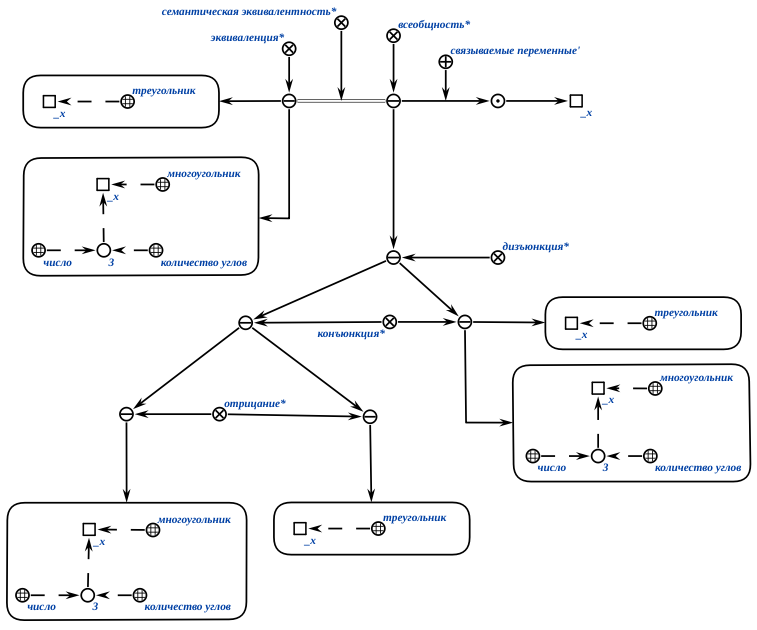
\includegraphics[scale=0.8]{author/part2/figures/logic/equivalence_representation.png}
	\label{fig:equivalence_representation}
\end{figure}

\begin{SCn}
\scnheader{квантор}
\scnsubset{логическая связка*}
\end{SCn}

\textbf{\textit{квантор}} — это \textit{отношение}, каждая связка которого истинна (или имеет истинную интерпретацию) при выполнении дополнительных условий, связанных с некоторыми из переменных, входящих в состав \textit{логических формул}, входящих в ее состав.

Будем говорить, что переменные связаны \textbf{\textit{квантором}} или попадают под область действия данного \textbf{\textit{квантора}} (имея в виду конкретную связку конкретного \textbf{\textit{квантора}}).

В состав каждой связки каждого \textbf{\textit{квантора}} входит \textit{атомарная формула}, являющаяся \textit{тривиальной структурой}, в которой перечислены переменные, связанные данным \textbf{\textit{квантором}}.

\begin{SCn}
\scnheader{всеобщность*}
\scnidtf{квантор всеобщности*}
\scnidtf{квантор общности*}
\scniselement{квантор}
\scniselement{ориентированное отношение}
\scniselement{класс связок разной мощности}
\end{SCn}

\textbf{\textit{всеобщность*}} --- это \textit{квантор}, для каждой связки которого, истинной в рамках некоторой \textit{формальной теории} (или имеющей истинную интерпретацию), выполняется следующее утверждение: все формулы, входящие в состав этой связки имеют соответствующую истинную интерпретацию в рамках этой же \textit{формальной теории} при всех (любых) возможных значениях всех элементов множества \textit{связываемых переменных\scnrolesign} входящего в эту связку.

Каждая связка \textit{квантора} \textbf{\textit{всеобщность*}} может быть представлена как \textit{конъюнкция*} (потенциально бесконечная) исходных \textit{логических формул}, входящих в состав этой связки, в каждой из которых все \textit{связанные переменные\scnrolesign} заменены на их возможные значения.

Квантор \textbf{\textit{всеобщности*}} зачастую обозначается ``$\forall$'' и читается как ``для всех'', ``для каждого'', ``для любого'' или ``все'', ``каждый'', ``любой''.

\begin{figure}[H]
\caption{Формализация примера всеобщности}
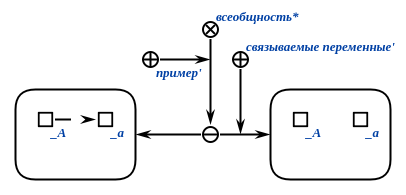
\includegraphics[scale=0.8]{author/part2/figures/logic/universality.png}
\label{fig:universality}
\end{figure}

\begin{SCn}
\scnheader{формула существования}
\scnidtf{существование*}
\begin{scnrelfromset}{разбиение}
	\scnitem{атомарное существование}
	\scnitem{неатомарное существование*}
\end{scnrelfromset}

\scnheader{неатомарное существование*}
\scnidtf{квантор неатомарного существования*}
\scniselement{квантор}
\scniselement{ориентированное отношение}
\scniselement{класс связок разной мощности}
\end{SCn}

\textbf{\textit{неатомарное существование*}} --- это \textit{квантор}, для каждой связки которого, истинной в рамках некоторой \textit{формальной теории} (или имеющей истинную интерпретацию), выполняется следующее утверждение: существуют значения всех элементов множества \textit{связываемых переменных\scnrolesign} входящего в эту связку, такие, что все формулы, входящие в состав этой связки имеют соответствующую истинную интерпретацию в рамках этой же \textit{формальной теории}.

Каждая связка \textit{квантора} \textbf{\textit{неатомарное существование*}} может быть представлена как \textit{дизъюнкция*} (потенциально бесконечная) исходных \textit{логических формул}, входящих в состав этой связки, в каждой из которых все \textit{связанные переменные\scnrolesign} заменены на их возможные значения.

Квантор \textbf{\textit{существования*}} зачастую обозначается ``$\exists$'' и читается как ``существует'', ``для некоторого'', ``найдется''.

\begin{figure}[H]
\caption{Формализация примера неатомарного существования}
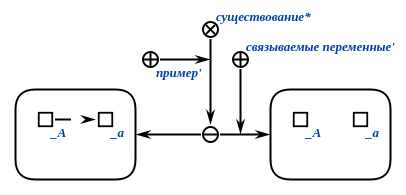
\includegraphics[scale=0.8]{author/part2/figures/logic/non_atomicExistence.png}
\label{fig:non_atomic_existence}
\end{figure}

\begin{SCn}
\scnheader{число значений переменной}
\scniselement{параметр}
\end{SCn}

Каждый элемент \textit{параметра} \textbf{\textit{число значений переменной}} представляет собой класс ориентированных пар, первым компонентом которых является знак \textit{логической формулы}, вторым --- \textit{sc-переменная}, имеющая в рамках данной \textit{логической формулы} ограниченное известное число значений, при которых данная формула является истинной в рамках соответствующей \textit{формальной теории}.

Отметим, что в случае \textit{атомарной логической формулы} каждая такая связка связывает знак формулы и знак принадлежащей ей \textit{sc-переменной}, то есть является, по сути, частным случаем пары принадлежности. В случае \textit{неатомарной логической формулы} указанная \textit{sc-переменная} может принадлежать любой из \textit{подформул*} исходной формулы.

\textit{измерением*} значения параметра \textbf{\textit{число значений переменной}} является некоторое \textit{число}, задающее количество значений \textit{sc-переменных} в рамках \textit{логической формулы}.

\begin{SCn}
\scnheader{кратность существования}
\scniselement{параметр}
\scnrelfrom{область определения параметра}{формула существования}
\scnhaselement{единственное существование}
\end{SCn}

Каждый элемент \textit{параметра} \textbf{\textit{кратность существования}} представляет собой класс логических \textit{формул существования}, для которых  при интерпретации на соответствующей \textit{предметной области} существует ограниченное общее для всех таких формул число комбинаций значений переменных, при которых указанные формулы являются истинными в рамках соответствующей \textit{формальной теории}.
\textit{измерением*} каждого значения \textbf{\textit{кратности существования}} является некоторое \textit{число}, задающее количество таких комбинаций.

\begin{SCn}
\scnheader{единственное существование}
\scnidtf{однократное существование}
\scnidtf{формула существования и единственности}
\end{SCn}

Единственное существование зачастую обозначается ``$\exists!$'' и читается как ``существует и единственный''.

\begin{SCn}
\scnheader{логическая формула и единственность}
\scnsubset{логическая формула}
\scnsubset{единственное существование}
\end{SCn}

Каждый элемент множества \textbf{\textit{логическая формула и единственность}} представляет собой \textit{логическую формулу} (\textit{атомарную} или \textit{неатомарную}), для которой дополнительно уточняется, что при ее интерпретации на некоторой предметной области существует только один набор значений переменных, входящих в эту формулу (или ее \textit{подформулы*}), при котором указанная логическая формула истинна в рамках \textit{формальной теории}, в которую входит данная \textit{предметная область}.


%\scnfilescg{figures/sd_logical_formulas/unique_existance.png}
%Данная формула показывает, что в рамках формальной теории геометрии Евклида существует только один прямоугольный треугольник с некоторым периметром, являющийся равнобедренным.

\textbf{\textit{связываемые переменные\scnrolesign}} --- это \textit{ролевое отношение}, которое связывает связку конкретного \textit{квантора} с множеством переменных, которые связаны этим квантором.

\textbf{\textit{открытая логическая формула}} --- это \textit{логическая формула}, в рамках которой (и всех ее \textit{подформул*}) существует хотя бы одна переменная, не связанная никаким \textit{квантором}.

\textbf{\textit{замкнутая логическая формула}} --- это \textit{логическая формула}, в рамках которой (и всех ее \textit{подформул*}) не существует переменных, не связанных каким-либо \textit{квантором}.

%\scnheader{Примеры неатомарных логических формул}
%\scneqtoset{\scgfileitem{figures/sd_logical_formulas/example_line_segment_sum.png}\\
%\scnrelfrom{описание примера}{
%\scnfilescg{figures/sd_logical_formulas/example_line_segment_sum_note.png}}
%\scnexplanation{AB+BC=AC}
%;
%\scgfileitem{figures/sd_logical_formulas/example_line_segment_diff.png}\\
%\scnrelfrom{описание примера}{
%\scnfilescg{figures/sd_logical_formulas/example_line_segment_diff_note.png}}
%\scnexplanation{AB-AC=CB}

\section{Смысловое представление логических формул и высказываний в прикладных логиках}
\label{sec_applied_logic}
\begin{SCn}
	\begin{scnrelfromlist}{ключевое понятие}
		\scnitem{иррефлексивное слотовое бинарное отношение}
		\scnitem{иррефлексивное неслотовое бинарное отношение}
		\scnitem{рефлексивное слотовое бинарное отношение}
		\scnitem{рефлексивное неслотовое бинарное отношение}
		\scnitem{транзитивное слотовое бинарное отношение}
		\scnitem{транзитивное неслотовое бинарное отношение}
		\scnitem{симметричное слотовое бинарное отношение}
		\scnitem{симметричное неслотовое бинарное отношение}
		\scnitem{антисимметричное слотовое бинарное отношение}
		\scnitem{антисимметричное неслотовое бинарное отношение}
		\scnitem{монотонное бинарное отношение*}
		\scnitem{отношение порядка монотонного отношения\scnrolesign}
		\scnitem{монотонное бинарное отношение\scnrolesign}
		\scnitem{монотонное слотовое бинарное отношение*}
		\scnitem{монотонное неслотовое бинарное отношение*}
		\scnitem{слотовое бинарное отношение}
		\scnitem{неслотовое бинарное отношение}
		\scnitem{слотовое отношение эквивалентности}
		\scnitem{неслотовое отношение эквивалентности}
		\scnitem{слотовое отношение нестрогого порядка}
		\scnitem{неслотовое отношение нестрогого порядка}
		\scnitem{секвенция}
		\scnitem{метаструктура}
		\scnitem{модальный оператор}
		\scnitem{модальное правило вывода}
		\scnitem{отношение становления структур}
		\scnitem{последовательность мышления}
		\scnitem{последовательность рационального мышления}
		\scnitem{последовательность иррационального мышления}
		\scnitem{последовательность рационального мышления классической логики}
		\scnitem{последовательность рационального дедуктивного мышления классической логики}
		\scnitem{последовательность рационального дедуктивного мышления классической логики на конечных sc-множествах}
		\scnitem{последовательность классического рационального дедуктивного познания}
	\end{scnrelfromlist}
\end{SCn}
\begin{SCn}
	\begin{scnrelfromlist}{ключевой знак}
		\scnitem{Отношение выводимости}
		\scnitem{Отношение выводимости на конечных множествах}
		\scnitem{Отношение выводимости на конечных множествах полносвязно представленных множеств}
		\scnitem{Отношение выводимости на секвенциях}
	\end{scnrelfromlist}
\end{SCn}

Прикладные логики (см. \scncite{Klini1973}, \scncite{Gribomon1990}, \scncite{Dragalin}, \scncite{Vagin2008}, \scncite{Gribomon1998}, \scncite{Golenkov2001b}) рассматривают приложения классической логики к абстрактным и предметным областям, описывающим действительность: логические теории об отношениях равенства и порядка (см. \scncite{Klini1973}, \scncite{Gribomon1990}), логические теории арифметики (см. \scncite{Klini1973}), логические теории времени (см. \scncite{Gribomon1998}, \scncite{Vagin2008}), логические теории доказательств (см. \scncite{Dragalin}, \scncite{Klini1973}), теории графов и геометрические теории (см. \scncite{Golenkov2001b}), теории природных и социальных систем (см. \scncite{Gribomon1990}).

Классификация логических теорий соответствует классификации предметных областей.
Рассмотрим некоторые понятия и примеры, которые рассматриваются в рамках прикладных логик.

\begin{SCn}
	\scnheader{слотовое бинарное отношение}
	\scnnote{Слотовое бинарное отношение --- слотовое sc-отношение, являющееся множеством.}
\end{SCn}
\begin{SCn}
	\scnheader{неслотовое бинарное отношение}
	\scnnote{Неслотовое бинарное отношение --- бинарное sc-отношение, являющееся множеством, но не являющееся слотовым sc-отношением.}
\end{SCn}
\begin{SCn}
	\scnheader{иррефлексивное слотовое бинарное отношение}
	\scnsubset{иррефлексивное бинарное отношение}
	\scnnote{Иррефлексивное слотовое бинарное отношение --- слотовое (бинарное) отношение, любая связка которого не является связкой,обозначенной петлевой дугой (дугой с совпадающим началом и концом).}
\end{SCn}
\begin{SCn}
	\scnheader{иррефлексивное неслотовое бинарное отношение}
	\scnsubset{иррефлексивное бинарное отношение}
	\scnnote{Иррефлексивное неслотовое бинарное отношение --- неслотовое бинарное sc-отношение, для любой связки которого ее различные принадлежности являются принадлежностями различных элементов.}
\end{SCn}
\begin{SCn}
	\scnheader{рефлексивное слотовое бинарное отношение}
	\scnsubset{рефлексивное бинарное отношение}
	\scnnote{Рефлексивное слотовое бинарное отношение --- слотовое бинарное sc-отношение, для любого элемента связки которого найдется связка, обозначенная петлевой дугой (дугой с совпадающим началом и концом).}
\end{SCn}
\begin{SCn}
	\scnheader{рефлексивное неслотовое бинарное отношение}
	\scnsubset{рефлексивное бинарное отношение}
	\scnnote{Рефлексивное неслотовое бинарное отношение --- неслотовое бинарное sc-отношение, для любого элемента связки которого найдется связка, имеющая две различные принадлежности этого элемента.}
\end{SCn}
\begin{SCn}
	\scnheader{транзитивное слотовое бинарное отношение}
	\scnsubset{транзитивное бинарное отношение}
	\scnnote{Транзитивное слотовое бинарное отношение --- слотовое бинарное отношение, для любых двух связок которого, конец одной из которых является началом второй, существует связка началом которой является начало первой связки, а концом является конец второй связки.}
\end{SCn}
\begin{SCn}
	\scnheader{транзитивное неслотовое бинарное отношение}
	\scnsubset{транзитивное бинарное отношение}
	\scnnote{Транзитивное неслотовое бинарное отношение --- неслотовое бинарное отношение, для которого существует ролевое отношение, первым доменом которого является это бинарное отношение такое, что для любых двух связок этого бинарного отношения, принадлежность элемента одной из которых не принадлежит этому ролевому отношению, а принадлежность этого же элемента второй связке принадлежит этому ролевому отношению, существует связка с принадлежностью элемента, принадлежащей ролевому отношению, принадлежность которого первой связке принадлежит ролевому отношению, и с принадлежностью элемента, не принадлежащей ролевому отношению, принадлежность которого второй связке не принадлежит этому ролевому отношению.}
\end{SCn}
\begin{SCn}
	\scnheader{симметричное слотовое бинарное отношение}
	\scnsubset{симметричное бинарное отношение}
	\scnnote{Симметричное слотовое бинарное отношение --- слотовое бинарное отношение, для любой связки которого существует связка, конец которой является началом первой связки, а начало --- ее концом (то есть эти связки обозначены встречными дугами).}
\end{SCn}
\begin{SCn}
	\scnheader{симметричное неслотовое бинарное отношение}
	\scnsubset{симметричное бинарное отношение}
	\scnnote{Симметричное неслотовое бинарное отношение --- неслотовое бинарное отношение, для которого существует ролевое отношение, первым доменом которого является это бинарное отношение, для любой связки которого существует связка с принадлежностью элемента первой связке, принадлежащая ролевому отношению, принадлежность которого второй связке не принадлежит этому ролевому отношению, и с принадлежностью элемента первой связке, не принадлежащая ролевому отношению, принадлежность которого второй связке принадлежит этому же ролевому отношению.}
\end{SCn}
\begin{SCn}
	\scnheader{антисимметричное слотовое бинарное отношение}
	\scnsubset{антисимметричное бинарное отношение}
	\scnnote{Антисимметричное слотовое бинарное отношение --- слотовое бинарное отношение, для любой связки которого у которой различным начало и конец не существует связки, конец которой является началом первой связки, а начало --- ее концом (то есть эти связки обозначены встречными дугами).}
\end{SCn}
\begin{SCn}
	\scnheader{антисимметричное неслотовое бинарное отношение}
	\scnsubset{антисимметричное бинарное отношение}
	\scnnote{Антисимметричное неслотовое бинарное отношение --- неслотовое бинарное отношение, для которого существует ролевое отношение, первым доменом которого является это бинарное отношение, для любой связки которого не существует связки с принадлежностью элемента первой связке, принадлежащая ролевому отношению, принадлежность которого второй связке не принадлежит этому ролевому отношению, и с принадлежностью другого элемента первой связке, не принадлежащая ролевому отношению, принадлежность которого второй связке принадлежит этому же ролевому отношению.}
\end{SCn}
\begin{SCn}
	\scnheader{монотонное слотовое бинарное отношение*}
	\scnsubset{монотонное бинарное отношение*}
	\scnnote{Монотонное слотовое бинарное отношение* --- слотовое бинарное отношение по отношению к отношению порядка, если есть связка этого бинарного отношения, то для любой его связки, начало которой связано связкой этого отношения порядка с началом первой, найдется третья связка бинарного отношения, начало которой совпадает с началом втором связки, а конец совпадает с концом первой.}
\end{SCn}
\begin{SCn}
	\scnheader{отношение порядка монотонного отношения\scnrolesign}
	\scnrelfrom{первый домен}{монотонное бинарное отношение*}
	\scnrelfrom{второй домен}{отношение порядка}
\end{SCn}
\begin{SCn}
	\scnheader{монотонное бинарное отношение\scnrolesign}
	\scnrelfrom{первый домен}{монотонное бинарное отношение*}
	\scnrelfrom{второй домен}{монотонное бинарное отношение}
\end{SCn}
\begin{SCn}
	\scnheader{монотонное неслотовое бинарное отношение*}
	\scnsubset{монотонное бинарное отношение*}
	\scnnote{Монотонное неслотовое бинарное отношение* --- неслотовое бинарное отношение по отношению к отношению порядка, для которого существует ролевое отношение, первым доменом которого является это бинарное отношение, такое, что если есть связка этого бинарного отношения, то для любой его связки элемент принадлежащий ей под этим ролевым отношением в отличие от другого связан связкой этого отношения порядка с элементом принадлежащим первой связки под этим же ролевым отношением, в отличие от другого элемента первой связки, найдется третья связка бинарного отношения такая, что элемент, принадлежащий ей под ролевым отношением, принадлежит под этим же ролевым отношением второй связке, а элемент, принадлежащий не под ролевым отношением третьей связке, принадлежит не под ролевым отношением первой связке.}
\end{SCn}
\begin{SCn}
	\scnheader{слотовое отношение эквивалентности}
	\scnsubset{sc-отношение эквивалентности}
	\scnnote{Слотовое отношение эквивалентности --- слотовое транзитивное бинарное отношение, которое является слотовым рефлексивным и симметричным отношением.}
\end{SCn}
\begin{SCn}
	\scnheader{неслотовое отношение эквивалентности}
	\scnsubset{sc-отношение эквивалентности}
	\scnnote{Неслотовое отношение эквивалентности --- неслотовое транзитивное бинарное отношение, которое является неслотовым рефлексивным и симметричным отношением (по соответствующим доменам).}
\end{SCn}
\begin{SCn}
	\scnheader{слотовое отношение нестрогого порядка}
	\scnsubset{sc-отношение нестрогого порядка}
	\scnnote{Слотовое отношение нестрогого порядка --- транзитивное бинарное отношение, которое является рефлексивным и антисимметричным.}
\end{SCn}
\begin{SCn}
	\scnheader{неслотовое отношение нестрогого порядка}
	\scnsubset{sc-отношение нестрогого порядка}
	\scnnote{Неслотовое отношение нестрогого порядка --- транзитивное бинарное отношение, которое является рефлексивным и антисимметричным (по соответствующим доменам).}
\end{SCn}

\begin{SCn}
	\scnheader{Отношение выводимости}
	\scnsuperset{Отношение выводимости на конечных множествах}
	\begin{scnindent}
		\scnsuperset{Отношение выводимости на конечных множествах полносвязно представленных множеств}
	\end{scnindent}
	\scniselement{рефлексивное бинарное отношение}
	\scniselement{транзитивное бинарное отношение}
	\scniselement{монотонное бинарное отношение}	
	\scnnote{Отношение выводимости --- рефлексивное, транзитивное, монотонное бинарное отношение на множествах посылок (высказываний, логических формул). Свойствами отношения выводимости являются правила вывода по Генцену.}
\end{SCn}

\begin{SCn}
	\scnheader{секвенция}
	\scnnote{секвенция --- связка (импликативного вида) между конъюнктивным множеством логических формул (конъюнкцией) и дизъюнктивным множеством логических формул (дизъюнкцией). Примером секвенции является выражение вида: $A_{1} \wedge A_{2} \wedge ... \wedge A_{n} \Rightarrow \ C_{1} \vee C_{2} \vee ... \vee C_{m}$.}
\end{SCn}

\begin{SCn}
	\scnheader{антецедент\scnrolesign}
	\scnrelfrom{первый домен}{секвенция}
	\scnrelfrom{второй домен}{конъюнкция}
\end{SCn}

\begin{SCn}
	\scnheader{консеквент\scnrolesign}
	\scnrelfrom{первый домен}{секвенция}
	\scnrelfrom{второй домен}{дизъюнкция}
\end{SCn}

\begin{SCn}
	\scnheader{Отношение выводимости на секвенциях}
	\scnnote{Отношение выводимости на секвенциях удовлетворяет правилам вывода исчисления секвенций.}
\end{SCn}

\begin{SCn}
	\scnheader{метаструктура}
	\scnnote{метаструктура --- структура, полносвязно представленным элементом которой является другая структура.}
\end{SCn}

\begin{SCn}
	\scnheader{модальный оператор}
	\scnnote{модальный оператор --- логическая связка, которая связывает логическую формулу со структурой (и иногда --- другими элементами) в метаструктуре. Примером модального оператора является оператор знания: $\mathrm{\Delta}$.}
\end{SCn}

\begin{SCn}
	\scnheader{модальное правило вывода}
	\scnnote{модальное правило вывода --- связка модального оператора формулы истинна (имеет истинную интерпретацию) в структуре, если и только если формула истинна (имеет истинную интерпретацию) в предшествующей ей структуре. Примером правила вывода является оператор знания: $\Gamma \cup \left\lbrace \alpha \right\rbrace \vdash \Gamma \cup \left\lbrace \mathrm{\Delta} \alpha \right\rbrace$.}
\end{SCn}

\begin{SCn}
	\scnheader{отношение становления структур}
	\scnnote{Отношение становления структур --- бинарное отношение на множестве структур, имеющих непустой общий носитель. Ролями в связке отношения становления являются ролевые отношения предшествующей структуры и последующей структуры.}
\end{SCn}

\begin{SCn}
	\scnheader{последовательность мышления}
	\scnidtf{судьба мышления}
	\scnidtf{мысль}	
	\scnnote{последовательность мышления --- последовательность sc-множеств высказываний (логических формул).}
	\begin{scnsubdividing}
		\scnitem{последовательность иррационального мышления}
		\scnitem{последовательность рационального мышления}
	\end{scnsubdividing}
\end{SCn}
\begin{SCn}
	\scnheader{последовательность рационального мышления классической логики}
	\scnidtf{судьба рационального мышления классической логики}
	\scnsubset{последовательность рационального мышления}
	\scnnote{последовательность рационального мышления --- последовательность (заданная отношением становления структур) (классически) непротиворечивых sc-множеств (sc-подмножеств или sc-надмножеств) высказываний.}
\end{SCn}
\begin{SCn}
	\scnheader{последовательность классического рационального дедуктивного мышления}
	\scnsubset{последовательность рационального мышления классической логики}
	\scnsuperset{последовательность рационального дедуктивного мышления классической логики на конечных sc-множествах}
	\scnnote{последовательность классического рационального дедуктивного мышления --- последовательность рационального мышления, последовательность (становления) непротиворечивых sc-множеств высказываний, дедуктивно логически следующих (по классическим правилам) друг за другом.}
\end{SCn}
\begin{SCn}
	\scnheader{последовательность классического рационального дедуктивного познания}
	\scnidtf{воля}
	\scnnote{последовательность классического рационального дедуктивного познания --- последовательность (заданная отношением становления структур) непротиворечивых sc-надмножеств высказываний, логически следующих друг за другом.}
\end{SCn}

\section{Смысловое представление логических формул и высказываний в неклассических логиках}
\label{sec_nonclass_logic}

\begin{SCn}
	\begin{scnrelfromlist}{ключевое понятие}
		\scnitem{немонотонный вывод на конечном sc-множестве посылок}
		\scnitem{выводимое множество}
		\scnitem{нечеткая истинность*}
		\scnitem{конструктивно истинное высказывание*}
		\scnitem{верное высказывание*}
		\scnitem{неискаженное высказывание*}
	\end{scnrelfromlist}
\end{SCn}

\textbf{\textit{неклассические логики}} (см. \scncite{Gribomon1990}, \scncite{Gribomon1998}, \scncite{Dragalin}, \scncite{Tarasov2007}, \scncite{Cintula2011}, \scncite{Vagin2008}) рассматривают (1) неклассический вывод, в котором отношение выводимости обладает иными свойствами (см. \scncite{Gribomon1990}, \scncite{Gribomon1998}, \scncite{Vagin2008}, \scncite{Dragalin}) и при котором можно или нельзя вывести то, что выводимо в классической логике, а также (2) --- другие шкалы признаков логических формул, их интерпретаций и значений (см. \scncite{Tarasov2007}, \scncite{Cintula2011}), отличных от ложных и (достоверно) истинных.

\begin{SCn}
	\scnheader{немонотонный вывод на конечном sc-множестве посылок*}
	\scnnote{\textit{немонотонный вывод на конечном sc-множестве посылок*} --- \textit{отношение} между (конечными) \textit{sc-множествами} истинных \textit{логических высказываний} (посылок). Если не существует вложения структуры \textit{атомарной логической формулы} в реляционную структуру (sc-подмножество предметной области) \textit{sc-множества} истинных (непротиворечивых) посылок и относительно них истинно отрицание этой \textit{атомарной формулы}, то существует \textit{sc-множество}, с принадлежащей ему реляционной структурой, включающей все элементы ранее упомянутой реляционной структуры и константы этой \textit{атомарной формулы}, которому принадлежат все посылки ранее упомянутого sc-множества истинных (непротиворечивых) посылок и упомянутая атомарная логическая формула.}
\end{SCn}

\begin{SCn}
	\scnheader{выводимое множество}
	\scnnote{\textit{выводимое множество} --- \textit{ситуативное sc-множество} (см. \scncite{Ivashenko2014diss}, \scncite{Ivashenko2017}), (временная) принадлежность \textit{логических формул} которому устанавливается в порядке становления процесса вывода этих \textit{логических формул}.}
\end{SCn}

\begin{SCn}
	\scnheader{нечеткая истинность*}
	\scnnote{\textit{нечеткая истинность*} связывает конечное sc-множество с временными принадлежностями на конечном множестве конечных явлений принадлежности с высказыванием. На явлениях принадлежности задано конечное sc-подмножество sc-отношения становления (непосредственно прежде, непосредственно после), которое задает структуру соответствующих sc-подмножеств. Эта структура является ориентированным деревом. \textit{нечеткая истинность*} --- \textit{бинарное отношение} между (нечеткой) принадлежностью связки  \textit{высказывания} \textit{формальной теории} и конечного sc-множества и действительным числом от 0.0 до 1.0. Нечеткая истинность отрицания высказывания равна разности 1.0 и нечеткой истинности высказывания, принадлежащего отрицанию. \textit{нечеткая истинность*} \textit{конъюнкции*} высказываний не превышает минимума нечеткой истинности элементов этой конъюнкции и не ниже (граничного или драстического) произведения \textit{нечеткой истинности*} этих же элементов конъюнкции. 
	\textit{нечеткая истинность*} \textit{дизъюнкции*} не превышает (граничной или драстической) суммы \textit{нечеткой истинности*} элементов этой конъюнкции и не ниже максимума нечеткой истинности этих же элементов конъюнкции.
	\textit{нечеткая истинность*} \textit{атомарных высказываний} равна среднему арифметическому изоморфного вложения структуры \textit{высказывания} в каждое из sc-подмножеств конечного sc-множества, которые входят в структуру заданную sc-отношением становления.}
\end{SCn}

\begin{SCn}
	\scnheader{конструктивно истинное высказывание*}
	\scnnote{\textbf{\textit{конструктивно истинное высказывание*}} --- подмножество \textit{истинного высказывания*}. 
	Истинные \textit{атомарные логические формулы} или их истинные интерпретации --- конструктивно истинные, если и только если они имеют изоморфное вложение в предметную область, где все элементы вложения полносвязно представлены. 
	\textit{конъюнкция*} \textit{конструктивно истинных логических формул} (или имеющих соответствующие конструктивно истинные интерпретации) конструктивно истинна (или имеет конструктивно истинную соответствующую интерпретацию).
	\textit{дизъюнкция*} хотя бы одной \textit{конструктивно истинной логической формулы} (или имеющей соответствующую полную конструктивно истинную интерпретацию) конструктивно истинна (или имеет конструктивно истинную соответствующую интерпретацию).
	\textit{отрицание*} \textit{ложной логической формулы} (или имеющей ложную соответствующую интерпретацию) конструктивно истинное (или имеет конструктивно истинную интерпретацию).
	Если все \textit{логические формулы} в \textit{дизъюнкции*} ложны (имеют соответствующие ложные интерпретации), то и дизъюнкция ложна (имеет соответствующую ложную интерпретацию).
	\textit{отрицание*} \textit{ложной логической формулы} (или имеющей ложную соответствующую интерпретацию) конструктивно истинное (или имеет конструктивно истинную интерпретацию).
	\textit{импликация*} с ложной посылкой (или имеющей соответствующую ложную интерпретацию) конструктивна истинна (или имеет конструктивно истинную интерпретацию).
	\textit{импликация*} с конструктивно истинным следствием (или имеющим соответствующую конструктивно истинную интерпретацию) конструктивна истинна (или имеет конструктивно истинную интерпретацию).
	\textit{конструктивно истинная импликация*} (или имеющая конструктивно истинную интерпретацию) с конструктивно истинной посылкой (или имеющей соответствующую конструктивно истинную интерпретацию) имеет конструктивно истинное следствие (или имеющее соответствующую конструктивно истинную интерпретацию).
	\textit{конструктивно истинная импликация*} (или имеющая конструктивно истинную интерпретацию) с ложным следствием (или имеющим соответствующую ложную интерпретацию) имеет ложную посылку (или имеющую соответствующую ложную интерпретацию).
	Существование значений переменных для \textit{логической формулы} конструктивно истинно (или имеет соответствующую конструктивную истинную интерпретацию), если всеобщность значений переменных для этой \textit{логической формулы} конструктивно истинна (или имеет соответствующую конструктивную истинную интерпретацию).
	Если \textit{логическая формула} имеет только конструктивно истинные соответствующие интерпретации, то всеобщность значений переменной для этой \textit{логической формулы} конструктивно истинна (или имеет соответствующую конструктивно истинную интерпретацию).
}
\end{SCn}

\begin{SCn}
	\scnheader{верное высказывание*}
	\scnnote{\textit{верное высказывание*} --- \textit{высказывание}, которое является истинным или неискаженным.}	
\end{SCn}

\begin{SCn}
	\scnheader{неискаженное высказывание*}
	\scnnote{\textit{неискаженое высказывание*} --- \textit{высказывание}, верность или неверность которого не приводит к противоречию.}	
\end{SCn}

%\input{author/references}
\chapauthor{Никифоров С.А.\\Гойло А.А.}
\chapter{Языковые средства формального описания синтаксиса и денотационной семантики естественных языков в ostis-системах}
\chapauthortoc{Никифоров С.А.\\Гойло А.А.}
\label{chapter_lang}

\abstract{
    Аннотация к главе.

    Список доработок:
    \begin{textitemize}
        \item написать аннотацию;
        \item вставить отредактированный анализ из статьи (в частности, тут не нужно говорить про sem web и нужно убрать пару опасных высказываний, погорячился);
        \item формализовать все обобщенные правила,
        \item адекватное определения лексемы, пересмотреть термины для исклюения возможности появления омонимии / синонимии,
        \item примеры и пояснения,
        \item сказать что-то про отношения на лексемах,
        \item выделить пр. о. лексики,
        \item пройтись по подсказкам от плагина, поправит форматирование,
        \item формализовать пр. о..
    \end{textitemize}
    Список вопросов:
    \begin{textitemize}
        \item нужно ли фомрализвать все частные правила, их несколько десятков.
    \end{textitemize}
}

Проблема совместимости результатов исследований также остро стоит и в лингвистике -- науке, в которой существует множество различных теорий, часто несовместимых друг с другом.
В лингвистических исследованиях используются разные варианты разметки данных, нет одного подхода к структуризации корпусов текстов и различаются способы представления данных в них~\cite{Farrar2002ACO},~\cite{Chiarcos2012}.

В качестве решения проблемы несовместимости различных способов описания данных в лингвистике предлагались варианты стандартизации форматов такого описания.
Примером могут служить Text Encoding Initiative -- консорциум по стандартизации представления текстов в цифровом виде~\cite{Text_Encoding_Initiative} и гайдлайны экспертной группы по стандартизации представления языковых данных EAGLES (например, рекомендации по разметке корпусов текстов\cite{EAGLES_Recommendations}). Однако ни один из таких стандартов не получил распространения и не стал использоваться лингвистами повсеместно~\cite[p.~4]{Ide2010WhatDI}.

Вместо создания рекомендаций по разметке языкового материала в качестве более эффективного средства решения указанных выше проблем предлагается создание онтологий~\cite{schalley_2019},~\cite{mccrae_2015}. Помимо того, что онтология верхнего уровня для предметной области языкознания может служить связующим звеном между различными лингвистическими теориями, она также представляет собой формализованное описание лингвистических концептов, представленное в удобном для компьютеров формате, что обусловливает ее применимость в системах, способных понимать аннотированные языковые данные, совершать интеллектуальный поиск по корпусам текстов, а также потенциально выполнять анализ существующих лингвистических исследований~\cite{Farrar2002ACO}.

В качестве такой онтологии ПрО лингвистики выступает The General Ontology of Linguistic Description (GOLD)~\cite{gold}.
В этой онтологии формализованы наиболее базовые категории и отношения, используемые в лингвистике, а сама онтология интегрирована с онтологией верхнего уровня Suggested Upper Merged Ontology (SUMO)~\cite{pease_2002_sumo}. Авторы GOLD пишут, что создавали онтологию в первую очередь для того, чтобы решить проблему интероперабельности данных лингвистической типологии и для того, чтобы с ее помощью экспертные системы могли обрабатывать научные данные по естественным языкам -- т.е. целью создателей онтологии не являлось непосредственно решение задач из области обработки текстов на естественном языке~\cite{farrar_2003} (с.4).

Онтологией естественных языков, нацеленной непосредственно на использование при решении задач по обработке ЕЯ, является Ontologies of Linguistic Annotation (OLiA)~\cite{chiarcos-2012-ontologies}. Основной идеей онтологии является обеспечение совместимости разметки языковых данных, полученных в результате выполненного компьютерными системами анализа текстов на естественном языке с соответствующими им лингвистическими концептами из онтологии -- в отличие от других лингвистических онтологий, OLiA предоставляет не только инвентарь концептов и отношений, но и необходимую спецификацию интеграции этих элементов с разметкой языковых данных (например, в корпусах).~\cite[p.~4]{chiarcos-2012-ontologies}.

При создании онтологий естественного языка, встает вопрос о статусе спецификации лингвистической информации в таких онтологиях. Дж. Бейтман выделяет три типа онтологий в зависимости от интегрированности естественно-языковой информации в онтологию~\cite{Bateman_1997}:
\begin{enumerate}
    \item онтологии, представляющие собой абстрактную семантико-концептуальную репрезентацию знаний о мире, которая используется непосредственно в качестве денотационной семантики для синтаксиса и лексики естественного языка;
    \item онтологии, в которых есть отдельная спецификация денотационной семантики естественного языка, которая служит интерфейсом между синтаксисом естественных языков и собственно концептуальной онтологией;
    \item онтологии, представляющие собой абстрактную спецификацию знаний о реальном мире вне зависимости от ограничений естественного языка
\end{enumerate}

Популярность в сфере обработки естественного языка приобрел второй тип онтологии~\cite[p.~8]{Bateman_1997}, так как он, в отличие от третьего подхода, который совсем не формализует лингвистическую информацию, позволяет специфицировать больше информации о естественных языках. Так, одна из самых популярных онтологий, используемых в системах для обработки естественного языка, the Generalized Upper Model~\cite{Bateman2002TheGU}, является онтологией второго типа~\cite{Bateman_1997}.
П. Буителар и др. подчеркивают, что всем формальным онтологиям необходима связь с языковой информацией для решения таких задач как выделение информации из ЕЯ-текстов, автоматизированное заполнение онтологий и генерации текста на естественном языке~\cite{Buitelaar_2009}.

Так как использование онтологий в NLP позволяет задать семантику получаемым в результате обработки естественного языка данным и потенциально повысить качество NLP-анализа, начинается переход к созданию движимых онтологиями систем обработки естественных языков~\cite{Kostareva2016UsingOM},~\cite{nevzorova_2019}.
Онтологии естественного языка активно применяются для генерации ЕЯ-текстов на основе некоторой онтологии предметной области~\cite{cimiano-etal-2013-exploiting},~\cite{Bouayad_2014}.

Онтологический подход также используется в системах естественно-языковых запросов для баз данных, в которых запрос на естественном языке транслируется в язык запросов по онтологиям конкретных предметных областей, конструкции которого затем транслируются в SQL для обеспечения взаимодействия с реляционными базами данных~\cite{saha_2016}.

Кроме того, спецификация лингвистической информации в виде онтологий помогает решать задачу автоматизированного создания онтологий на основе естественно-языковых текстов~\cite{SHAMSFARD200417}.

Создаются онтологии частных областей лингвистики: например, онтология пространственных выражений в естественных языках~\cite{BATEMAN20101027}, онтология темпоральных сущностей на основе естественного языка~\cite{Moens_1987}, онтологии конкретных естественных языков~\cite{Dobrov_2018}.
При использовании онтологий для обработки естественного языка необходимо "связать"{} концепты из онтологии с лексикой конкретного ЕЯ.
Для этого создаются различные расширения существующих языковых БД, таких как WordNet~\cite{wordnet}, VerbNet~\cite{verbnet} и FrameNet~\cite{framenet}, направленные на их использование совместно с онтологиями верхнего уровня (например,~\cite{pease_fellbaum_2010}).
Активные разработки идут в сфере создания онтологий словарного состава естественных языков, в результате которых появилось множество формализованных описаний лексики~\cite{matsukawa-yokota-1991-development},~\cite{calzolari_1991},~\cite{buitelaar2006linginfo},~\cite{Cimiano2007LexOntoAM},~\cite{buitelaar_2006}.
Так как распространенные базы данных лексики ЕЯ не являются онтологиями и не имеют достаточной степени формализации (например, WordNet), создаются онтологии, являющиеся своего рода "надстройкой"{} над такими базами данных, самой известной из которых является lemon~\cite{McCrae_2012}.

Многие из приведенных выше онтологий созданы с использованием технологии Semantic Web~\cite{sem_web}, который является внешней технологией по отношению к существующим решениям для обработки естественных языков, поэтому последним приходится обращаться к ней с помощью API и стандартизированных языков запросов (в частности, SPARQL)~\cite{Bouayad_2014}.

Стоит отметить, что несмотря на активное развитие в направлении применения онтологий для обработки ЕЯ, многие популярные NLP-библиотеки (например, NLTK~\cite{nltk} и spaCy~\cite{spacy}) в принципе не поддерживают использование онтологий, а большинство инструментов для разметки естественно-языковых текстов используют обычно свой формат, что требует использования специфичных для таких инструментов парсеров и конвертеров, чтобы данные можно было применить при решении каких-либо задач~\cite[p.~3]{Erekhinskaya2020TenWO}.

Таким образом, в настоящее время в данной области можно выделить следующие проблемы:
\begin{enumerate}
    \item Отсутствие унификации (стандартизации) приведенных выше решений приводит к существенным накладным расходам на их интеграцию и значительно усложняет построение различных систем с их использованием в силу большой трудоемкости их интеграции~\cite{Standart2021},\cite{GolenkovProblems2021}.
    \item Несмотря на то, что онтологии потенциально способствуют решению широкого круга задач в сфере обработки естественного языка, большинство движимых онтологиями NLP-систем сконцентрированы на решении специализированных задач (например, только генерации текста, только заполнения онтологии или только обеспечения поиска с помощью естественного языка).
    \item Создано довольно большое количество частных лингвистических онтологий, формализующих, однако, лишь некий подраздел предметной области лингвистики (в особенности лексики), что отчасти вытекает из предыдущего пункта. В то же время, существующие лингвистические онтологии верхнего уровня (например, OLiA) все равно не до конца решают проблему унификации, т.к. им требуется вводить промежуточный уровень для интеграции полученных в результате NLP-анализа данных с фрагментами онтологии.
\end{enumerate}

Так как используемый в технологии OSTIS SC-код обладает достаточной экспрессивностью для описания знаний любого вида, а сама технология нацелена на создание интероперабельных интеллектуальных систем нового поколения, естественно-языковые интерфейсы ostis-систем смогут справляться с широким кругом задач по обработке текстов на естественных языках -- будь то синтез естественно-языковых текстов в целом, ведение диалога в диалоговых системах, поиск с использованием естественного языка, выделение информации из текстов и т.п. При этом в то время как в текущем состоянии сферы обработки естественных языков данные классы задач выполняются зачастую специализированными средствами и требуют дополнительных затрат на обеспечение потенциальной совместимости с конкретными компьютерными системами, в рамках технологии OSTIS для их решения будет использоваться один универсальный язык смыслового представления знаний, на котором будут написаны как компоненты решателя задач, так и онтология языков и конкретных предметных областей, что позволит решить проблему интероперабельности.

Более того, онтология естественных языков, разработанная в рамках такой технологии, могла бы быть использована не только для решения прикладных задач по обработке естественного языка, но и для обеспечения интероперабельности данных, полученных в ходе лингвистических исследований, что было бы ценным вкладом в область теоретической лингвистики.

Наконец, онтологию естественных языков можно рассматривать в качестве подмножества онтологии языков вообще (как естественных, так и искусственных и формальных), чего не делают рассмотренные выше существующие онтологии. Это позволит концептуализировать естественный язык в одной системе с языками программирования и более тесно связать используемые в соответствующих предметных областях понятия для более эффективного решения задач по обработке естественного языка в интеллектуальных компьютерных системах.

Цель данной работы -- предложить базовые средства формального описания синтаксиса и денотационной семантики различных языков в виде фрагмента онтологии языков и информационных конструкций, который можно будет использовать при проектировании интеллектуальных компьютерных систем нового поколения.
%Конец анализа

\section{Формализация естественных языков}

Как уже говорилось выше, для использования достижений лингвистики при проектировании интеллектуальных компьютерных систем требуется представить полученные результаты в формальном виде. В данном разделе мы предложим формализацию основных лингвистических концептов, выполненную на формальном языке представления знаний -- SC-коде.

\begin{SCn}

    \scnheader{язык}
    \begin{scnrelfromset}{разбиение}
        \scnitem{естественный язык}
        \begin{scnindent}
            \scntext{пояснение}{Естественный язык представляет собой язык, который не был создан целенаправленно}
        \end{scnindent}
        \scnitem{искусственный язык}
        \begin{scnindent}
            \scntext{пояснение}{Искусственный язык представляет собой язык, специально разработанный для достижения определённых целей}
            \scnhaselement{Эсперанто}
            \scnhaselement{Python}
            \scnsuperset{сконструированный язык}
            \begin{scnindent}
                \scntext{пояснение}{Сконструированный язык представляет собой искусственный язык, предназначенный для общения людей}
                \scnhaselement{Эсперанто}
            \end{scnindent}
        \end{scnindent}
    \end{scnrelfromset}

    \scnsuperset{международный язык}
    \begin{scnindent}
        \scntext{пояснение}{Международный язык представляет собой естественный или искусственный язык, использующийся для общения людей из разных стран}
        \scnhaselement{Английский язык}
        \scnhaselement{Русский язык}
    \end{scnindent}

    \scnheader{плановый язык}
    \begin{scnreltoset}{пересечение}
        \scnitem{сконструированный язык}
        \scnitem{международный язык}
    \end{scnreltoset}

    \scnheader{язык общения}
    \begin{scnreltoset}{объединение}
        \scnitem{естественный язык}
        \scnitem{сконструированный язык}
    \end{scnreltoset}
    \scnhaselement{Английский язык}
    \scnhaselement{Русский язык}
    \scnhaselement{Эсперанто}
    \begin{scnreltoset}{объединение}
        \scnitem{корневой язык}
        \begin{scnindent}
            \scntext{пояснение}{Корневой язык представляет собой язык, для которого характерно полное отсутствие словоизменения и наличие грамматической значимости порядка слов, состоящих только из корня.}
            \scnhaselement{Английский язык}
        \end{scnindent}
        \scnitem{агглютинативный язык}
        \begin{scnindent}
            \scntext{пояснение}{Агглютинативный язык характеризуется развитой системой употребления суффиксов, приставок, добавляемых к неизменяемой основе слова, которые используются для выражения категорий числа, падежа, рода и др.}
            \scnhaselement{Английский язык}
        \end{scnindent}
        \scnitem{флективный язык}
        \begin{scnindent}
            \scntext{пояснение}{Для флективного языка характерно развитое употребление окончаний для выражения категорий рода, числа, падежа, сложная система склонения глаголов, чередование гласных в корне, а также строгое различение частей речи.}
            \scnhaselement{Русский язык}
        \end{scnindent}
        \scnitem{профлективный язык}
        \begin{scnindent}
            \scntext{пояснение}{Для профлективного языка характерны агглютинация (в случае именного словоизменения), флексия и чередование гласных (аблаут)(в случае глагольного словоизменения).}
        \end{scnindent}
    \end{scnreltoset}

\end{SCn}

\section{Формализация синтаксиса естественных языков}

Лексема -- минимальная единица языка, имеющая семантическую интерпретацию и обозначающая концепт, отражающий взгляд на мир некоторого языкового сообщества \scncite{glossary}.

Грамматическая категория -- система противопоставленных друг другу рядов грамматических форм с однородными значениями. В рамках нашей формализации предлагается представить грамматические категории как классы ролевых отношений, каждый из которых соответствует определенному грамматическому значению. Следует отметить, что приводится онтология основных грамматических категорий, часто встречающихся в естественных языках, а не всех возможных.

\begin{SCn}

    \scnheader{грамматическая категория}
    \scnhaselement{лицо}
    \begin{scnindent}
        \scnrelto{семейство подмножеств}{ролевое отношение}
        \scnhaselement{первое лицо\scnrolesign}
        \scnhaselement{второе лицо\scnrolesign}
        \scnhaselement{третье лицо\scnrolesign}
    \end{scnindent}
    \scnhaselement{число}
    \begin{scnindent}
        \scnrelto{семейство подмножеств}{ролевое отношение}
        \scnhaselement{единственное число\scnrolesign}
        \scnhaselement{множественное число\scnrolesign}
        \scnhaselement{двойственное число\scnrolesign}
        \scnhaselement{тройственное число\scnrolesign}
        \scnhaselement{паукальное число\scnrolesign}
    \end{scnindent}
    \scnhaselement{род}
    \begin{scnindent}
        \scnrelto{семейство подмножеств}{ролевое отношение}
        \scnhaselement{мужской род\scnrolesign}
        \scnhaselement{средний род\scnrolesign}
        \scnhaselement{женский род\scnrolesign}
    \end{scnindent}
    \scnhaselement{падеж}
    \begin{scnindent}
        \scnrelto{семейство подмножеств}{ролевое отношение}
        \scnhaselement{именительный падеж\scnrolesign}
        \scnhaselement{родительный падеж\scnrolesign}
        \scnhaselement{дательный падеж\scnrolesign}
        \scnhaselement{винительный падеж\scnrolesign}
        \scnhaselement{творительный падеж\scnrolesign}
        \scnhaselement{предложный падеж\scnrolesign}
        \scnhaselement{звательный падеж\scnrolesign}
        \scnhaselement{абсолютивный падеж\scnrolesign}
        \scnhaselement{эргативный падеж\scnrolesign}
    \end{scnindent}
    \scnhaselement{время}
    \begin{scnindent}
        \scnrelto{семейство подмножеств}{ролевое отношение}
        \scnhaselement{настоящее время\scnrolesign}
        \scnhaselement{прошедшее время\scnrolesign}
        \scnhaselement{будущее время\scnrolesign}
    \end{scnindent}
    \scnhaselement{наклонение}
    \begin{scnindent}
        \scnrelto{семейство подмножеств}{ролевое отношение}
        \scnhaselement{изъявительное наклонение\scnrolesign}
        \scnhaselement{повелительное наклонение\scnrolesign}
        \scnhaselement{сослагательное наклонение\scnrolesign}
        \scnhaselement{условное наклонение\scnrolesign}
    \end{scnindent}
    \scnhaselement{залог}
    \begin{scnindent}
        \scnrelto{семейство подмножеств}{ролевое отношение}
        \scnhaselement{действительный залог\scnrolesign}
        \scnhaselement{страдательный залог\scnrolesign}
        \scnhaselement{средний залог\scnrolesign}
        \scnhaselement{возвратный залог\scnrolesign}
        \scnhaselement{взаимный залог\scnrolesign}
    \end{scnindent}
    \scnhaselement{вид}
    \begin{scnindent}
        \scnrelto{семейство подмножеств}{ролевое отношение}
        \scnhaselement{совершенный вид\scnrolesign}
        \scnhaselement{несовершенный вид\scnrolesign}
        \scnhaselement{общий вид\scnrolesign}
        \scnhaselement{прогрессивный вид\scnrolesign}
        \scnhaselement{перфектный вид\scnrolesign}
    \end{scnindent}
    \scnhaselement{степень сравнения}
    \begin{scnindent}
        \scnrelto{семейство подмножеств}{ролевое отношение}
        \scnhaselement{положительная степень сравнения\scnrolesign}
        \scnhaselement{сравнительная степень сравнения\scnrolesign}
        \scnhaselement{превосходная степень сравнения\scnrolesign}
    \end{scnindent}
\end{SCn}

Пример формализации части приведенных выше отношений на языке sc.g приведен на рисунке~\ref{fig:lexeme_example}.

\begin{figure}[h]
    \centering
    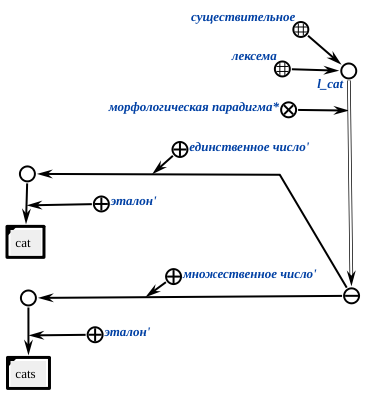
\includegraphics[width=0.4\textwidth]{images/part2/chapter_lang/lexeme_example.png}
    \caption{Пример спецификации лексемы в базе знаний.}
    \label{fig:lexeme_example}
\end{figure}

Часть речи -- категория, представляющая собой класс синтаксически эквивалентных знаков ЕЯ.

\begin{SCn}

    \scnheader{часть речи}
    \scnrelto{семейство подмножеств}{лексема}
    \scnhaselement{существительное}
    \scnhaselement{прилагательное}
    \scnhaselement{глагол}
    \scnhaselement{наречие}
    \scnhaselement{предлог}
    \scnhaselement{комплементатор}
    \scnhaselement{вспомогательный глагол}
    \scnhaselement{детерминант}

\end{SCn}

\textit{морфологическая парадигма*} - бинарное ориентированное отношение, связывающее лексему и множество ее словоформ.

Словоформа -- подмножество лексемы, которому принадлежат все вхождения лексемы с определенными грамматическими значениями. В рамках нашей онтологии словоформа понимается несколько иначе, чем принято в лингвистике, так как все вхождения лексемы в технологии OSTIS являются файлами.

При формализации синтаксиса в основном использовались стандартные положения генеративной грамматики \scncite{adger2003core}, \scncite{jackendoff1977x}, \scncite{haegeman1994introduction}, \scncite{carnie2012syntax}.

Дистрибуция знака –- это подмножество синтаксических правил, в которые входит данный знак.

Составляющая -- элемент множества C подмножеств кортежа вхождений лексем S, которое содержит в качестве элементов как сам S, так и все вхождения лексем в S, таким образом, что любые два подмножества, входящие в C, либо не пересекаются, либо одно из них включается в другое.

Непосредственно составляющая --  есть множество составляющих S, в которое входят составляющие A и B. В является непосредственно составляющей А если и только если В является подмножеством А и нет такой составляющей С, которая является подмножеством А и подмножеством которой является В.

Элементарная составляющая -- элемент кортежа вхождений лексем L, являющихся непосредственно составляющими множества составляющих C и не имеющих дочерних составляющих.

Синтаксическая группа -- класс составляющих, в который входят составляющие с вершинами, принадлежащими к одной части речи. Синтаксические группы представляют собой либо синглетон (минимально включают в себя вершину), либо упорядоченную пару, состояющую из вершины и другой синтаксической группы.

Вершина –- составляющая, дистрибуция которой совпадает с дистрибуцией всей синтаксической группы.

\begin{SCn}

    \scnheader{составляющая}
    \begin{scnrelfromset}{разбиение}
        \scnitem{синтаксическая группа}
        \scnitem{вершина}
    \end{scnrelfromset}

    \scnheader{синтаксическая группа}
% максимальная, промеж и вершины, вывести классы из примера как их пересечения
    \begin{scnrelfromset}{разбиение}
        \scnitem{именная группа}
        \begin{scnindent}
            \scntext{пояснение}{\textit{Именная группа} -- синтаксическая группа, вершиной которой является существительное.}
        \end{scnindent}
        \scnitem{глагольная группа}
        \begin{scnindent}
            \scntext{пояснение}{\textit{Глагольная группа} -- синтаксическая группа, вершиной которой является глагол.}
        \end{scnindent}
        \scnitem{группа прилагательного}
        \begin{scnindent}
            \scntext{пояснение}{\textit{Группа прилагательного} -- синтаксическая группа, вершиной которой является прилагательное.}
        \end{scnindent}
        \scnitem{наречная группа}
        \begin{scnindent}
            \scntext{пояснение}{\textit{Наречная группа} -- синтаксическая группа, вершиной которой является наречие.}
        \end{scnindent}
        \scnitem{предложная группа}
        \begin{scnindent}
            \scntext{пояснение}{\textit{Предложная группа} -- синтаксическая группа, вершиной которой является предлог.}
        \end{scnindent}
        \scnitem{группа комплементатора}
        \begin{scnindent}
            \scntext{пояснение}{\textit{Группа комплементатора} -- синтаксическая группа, вершиной которой является комплементатор.}
        \end{scnindent}
        \scnitem{временная группа}
        \begin{scnindent}
            \scntext{пояснение}{\textit{Временная группа} -- синтаксическая группа, вершиной которой является вспомогательный либо модальный глагол.}
        \end{scnindent}
        \scnitem{группа детерминанта}
        \begin{scnindent}
            \scntext{пояснение}{\textit{Группа детерминанта} -- синтаксическая группа, вершиной которой является детерминант.}
        \end{scnindent}
    \end{scnrelfromset}
    \begin{scnrelfromset}{разбиение}
        \scnitem{максимальная проекция вершины}
        \scnitem{промежуточная проекция вершины}
    \end{scnrelfromset}

\end{SCn}

При этом для упрощения могут быть введены более узкие классы, являющиеся пересечением приведенных выше, например \textit{максимальная проекция вершины группы детерминанта}.

\begin{SCn}

    \scnheader{максимальная проекция вершины группы детерминанта}
    \begin{scnreltoset}{пересечение}
        \scnitem{группа детерминанта}
        \scnitem{максимальная проекция вершины}
    \end{scnreltoset}

\end{SCn}

Пример синтаксической структуры предложения, записанный с применением введенных выше понятий представлен на рисунке~\ref{pic_tree}.

\begin{figure*}[h]
    \centering
    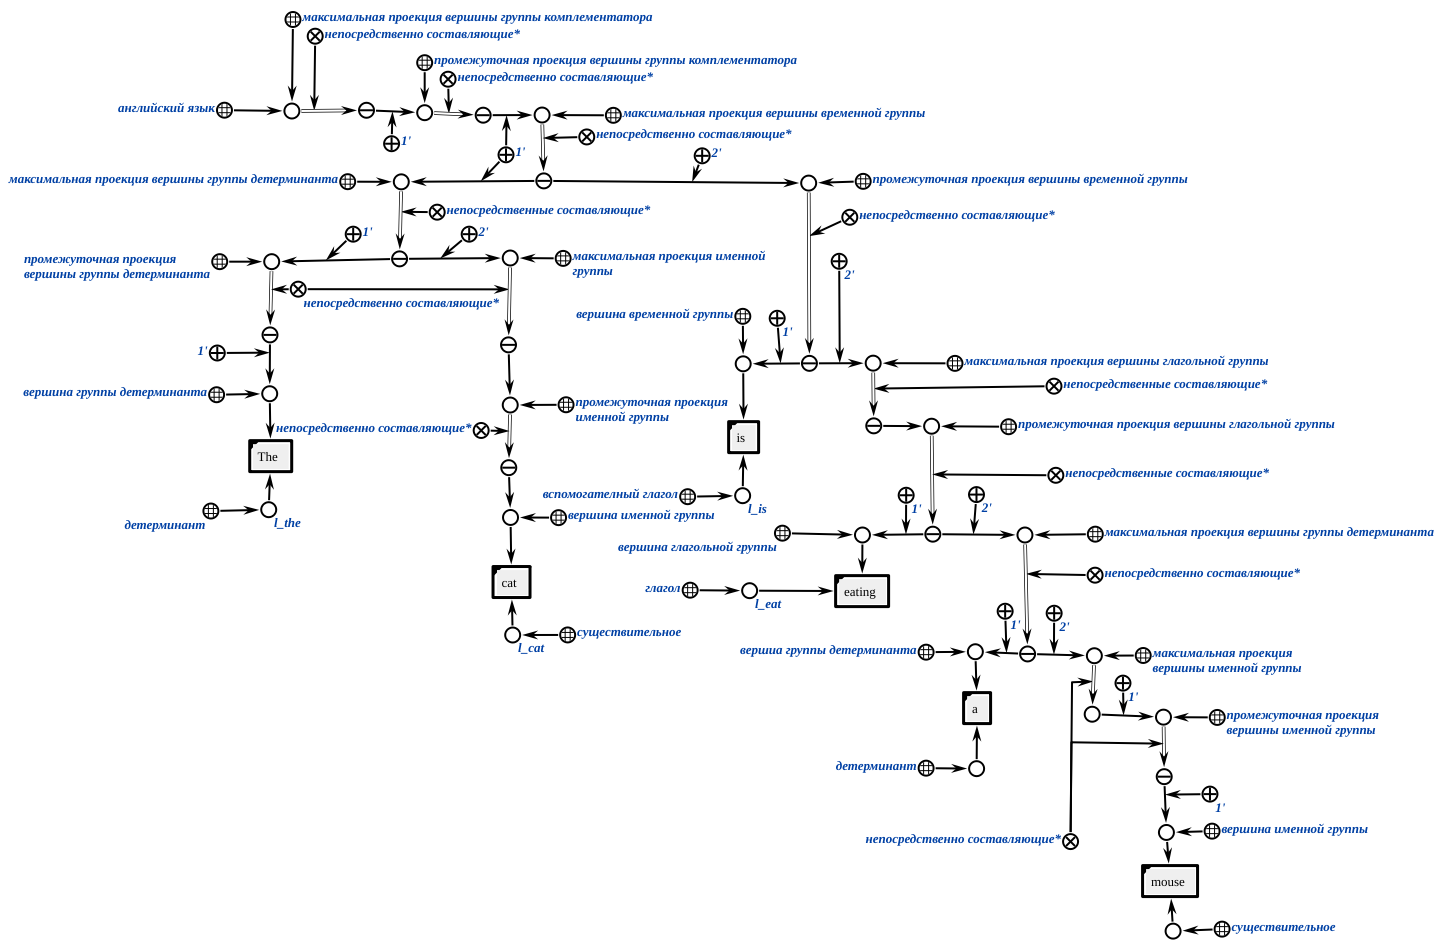
\includegraphics[width=\textwidth]{images/part2/chapter_lang/syntactic.png}
    \caption{Пример синтаксической структуры предложения.}
    \label{pic_tree}
\end{figure*}

Структуры синтаксических групп не являются произвольными -- элементы внутри группы могут граничить только с определенными множествами элементов.
Ниже приводятся возможные структуры синтаксических групп.
Знак "->"{} следует читать как "состоит из"{}.
В скобках указаны опциональные элементы.

Группа детерминанта:
\begin{textitemize}
    \item Максимальная проекция вершины группы детерминанта -> (Максимальная проекция вершины группы детерминанта) Промежуточная проекция вершины группы детерминанта
    \item Промежуточная проекция вершины группы детерминанта -> Вершина группы детерминанта (Максимальная проекция вершины именной группы)
\end{textitemize}

Именная группа:
\begin{textitemize}
    \item Максимальная проекция вершины именной группы -> (Максимальная проекция вершины группы детерминанта) Промежуточная проекция вершины именной группы
    \item Промежуточная проекция вершины именной группы -> (Максимальная проекция вершины группы прилагательного) Промежуточная проекция вершины именной группы ИЛИ Промежуточная проекция вершины именной группы (Максимальная проекция вершины предложной группы)
    \item Промежуточная проекция вершины именной группы -> Вершина именной группы (Максимальная проекция вершины предложной группы)
\end{textitemize}

Глагольная группа:
\begin{textitemize}
    \item Максимальная проекция вершины глагольной группы -> Промежуточная проекция вершины глагольной группы
    \item Промежуточная проекция вершины глагольной группы -> Промежуточная проекция вершины глагольной группы (Максимальная проекция вершины предложной группы) ИЛИ Промежуточная проекция вершины глагольной группы (Максимальная проекция вершины наречной группы)
    \item Промежуточная проекция вершины глагольной группы -> Вершина глагольной группы (Максимальная проекция вершины именной группы)
\end{textitemize}

Наречная группа:
\begin{textitemize}
    \item Максимальная проекция вершины наречной группы -> Промежуточная проекция вершины наречной группы
    \item Промежуточная проекция вершины наречной группы -> (Максимальная проекция вершины наречной группы) Промежуточная проекция вершины наречной группы
    \item Промежуточная проекция вершины наречной группы -> Вершина наречной группы (Максимальная проекция вершины предложной группы)
\end{textitemize}

Группа прилагательного:
\begin{textitemize}
    \item Максимальная проекция вершины группы прилагательного -> Промежуточная проекция вершины группы прилагательного
    \item Промежуточная проекция вершины группы прилагательного -> (Максимальная проекция вершины наречной группы) + Промежуточная проекция вершины группы прилагательного
    \item Промежуточная проекция вершины группы прилагательного -> Вершина группы прилагательного (Максимальная проекция вершины предложной группы)
\end{textitemize}

Предложная группа:
\begin{textitemize}
    \item Максимальная проекция вершины предложной группы -> Промежуточная проекция вершины предложной группы
    \item Промежуточная проекция вершины предложной группы -> Промежуточная проекция вершины предложной группы (Максимальная проекция вершины предложной группы) ИЛИ (Максимальная проекция вершины наречной группы) Промежуточная проекция вершины предложной группы
    \item Промежуточная проекция вершины предложной группы -> Вершина предложной группы (Максимальная проекция вершины именной группы)
\end{textitemize}

Временная группа:
\begin{textitemize}
    \item Максимальная проекция вершины временной группы -> (Максимальная проекция вершины группы детерминанта) Промежуточная проекция вершины временной группы
    \item Промежуточная проекция вершины временной группы -> Вершина временной группы (Максимальная проекция вершины глагольной группы)
\end{textitemize}

Группа комплементатора:
\begin{textitemize}
    \item Максимальная проекция вершины группы комплементатора -> (Максимальная проекция вершины некоторой синтаксической группы) Промежуточная проекция вершины группы комплементатора
    \item Промежуточная проекция вершины группы комплементатора -> Вершина группы комплементатора Максимальная проекция вершины временной группы
\end{textitemize}

В формальном виде данные правила можно представить следующим образом (см. рисунок~\ref{fig:pic_tree_structure_rule}).

\begin{figure*}[h]
    \centering
    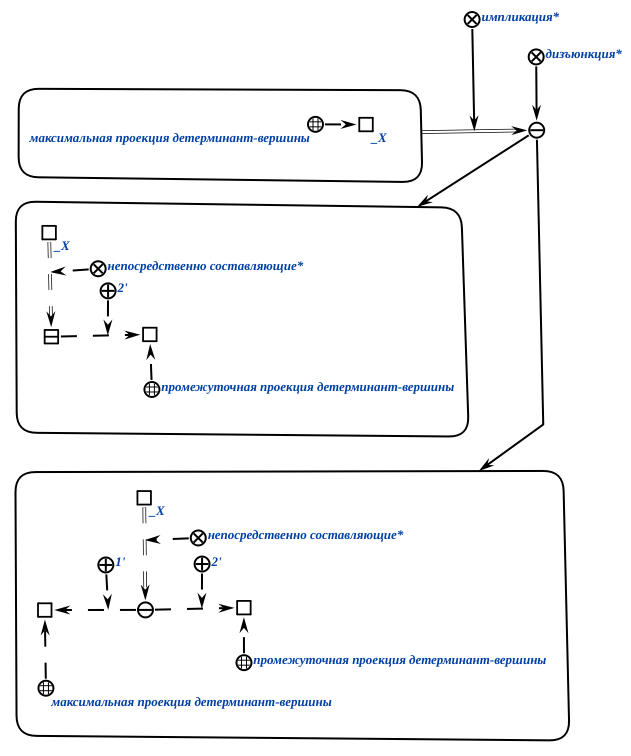
\includegraphics[width=0.8\textwidth]{images/part2/chapter_lang/tree_structure_rule.png}
    \caption{Пример правила структуры синтаксической группы.}
    \label{fig:pic_tree_structure_rule}
\end{figure*}

Комплемент -- синтаксическая группа, являющаяся сестрой вершины. Сестрами считаются составляющие, являющиеся непосредственно составляющими одной и той же составляющей.

Адъюнкт -- синтаксическая группа, являющаяся дочерью (непосредственно составляющей) промежуточной проекции и сестрой промежуточной проекции вершины той же синтаксической группы.

Спецификатор -- синтаксическая группа, являющейся дочерью максимальной проекции и сестрой промежуточной проекции.

Приведенные выше правила структуры синтаксических групп можно обобщить и свести к трем более абстрактным.

Правило спецификатора: XP -> (YP) X'

Правило адъюнкта: X' -> X' (ZP) | X' -> (ZP) X'

Правило комплемента: X' -> X (WP)

Формальное представление данных правил аналогично приведенному на рисунке~\ref{fig:pic_tree_structure_rule}.

\section{Формализация денотационной семантики естественных языков}

денотационная семантика языка специфицирует интерпретацию элементов синтаксиса данного языка и представляет собой множество формул, описывающих то, каким образом знаковым конструкциям языка ставятся в соответствие обозначаемые ими сущности и конфигурации отношений между этими сущностями.

денотационная семантика естественных языков должна обладать свойством композициональности -- т.е. интерпретация всего высказывания должна выводиться из интерпретации отдельных его частей. Таким образом, необходимо предоставить формальное описание интерпретации элементов синтаксиса ЕЯ, представленных в предыдущем разделе, а также описание правил совмещения интерпретации отдельных элементов для получения смысла всего высказывания.

В данной главе мы предлагаем вариант формализации денотационной семантики естественных языков в рамках \textit{Технологии OSTIS}, для составления которой использовались стандартные положения формальной семантики \scncite{heim1998semantics}, \scncite{Winter+2016}, \scncite{portner2008formal}.

Рассмотрим примеры правил, реализующих денотационную семантику языка. Приведенные ниже правила должны применяться последовательно и позволяют получить смысл текста естественного языка по его синтаксической структуре, "поднимаясь"{} по дереву составляющих от вершин к максимальным проекциям.

На рисунке~\textit{\nameref{fig:d_sem_1}} приведено правило, по которому происходит интерпретация вершин именной группы и группы прилагательного.
Смыслом таких вершин является класс, например: прилагательному ``черный'' соответствует множество черных объектов, а существительному ``кот'' -- множество котов.

\begin{figure}[H]
    \centering
    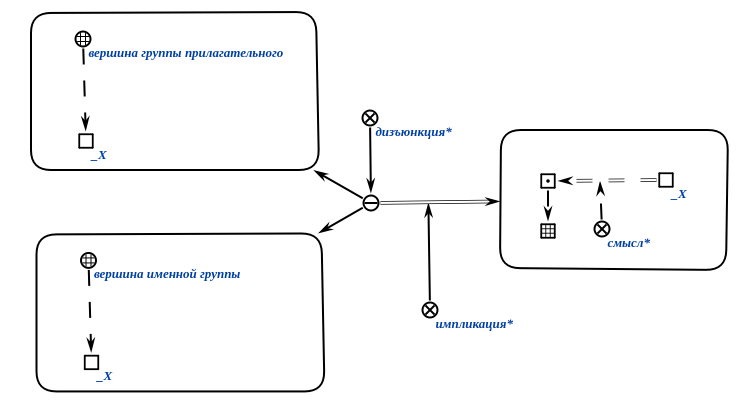
\includegraphics[width=0.8\textwidth]{images/part2/chapter_lang/d_sem_1}
    \caption{Правило интерпретации вершины группы прилагательного и вершины именной группы}
    \label{fig:d_sem_1}
\end{figure}
%в этом правиле мы интерпретируем вершины групп прилагательного и существительного - т.е. отдельные "слова"{}-прилагательные и существительные, которые у нас соответствуют классам

На рисунке~\textit{\nameref{fig:d_sem_2}} приведено правило, по которому происходит интерпретация именной группы, максимальная проекция которой включается в себя также группу прилагательного.
Как говорилось выше, для применения данного правила необходимо предварительное применение правила, представленного на рисунке~\textit{\nameref{fig:d_sem_1}}.
Смыслом таких конструкций является класс, являющийся результатом пересечения классов, полученных в результате интерпретации вершин групп прилагательного и именной группы по отдельности. Например: ``черный кот''{} -- множество черных котов, пересечение множества котов и черных объектов. %ну все, теперь включаю мою кошку в соавторы

\begin{figure*}[h]
    \centering
    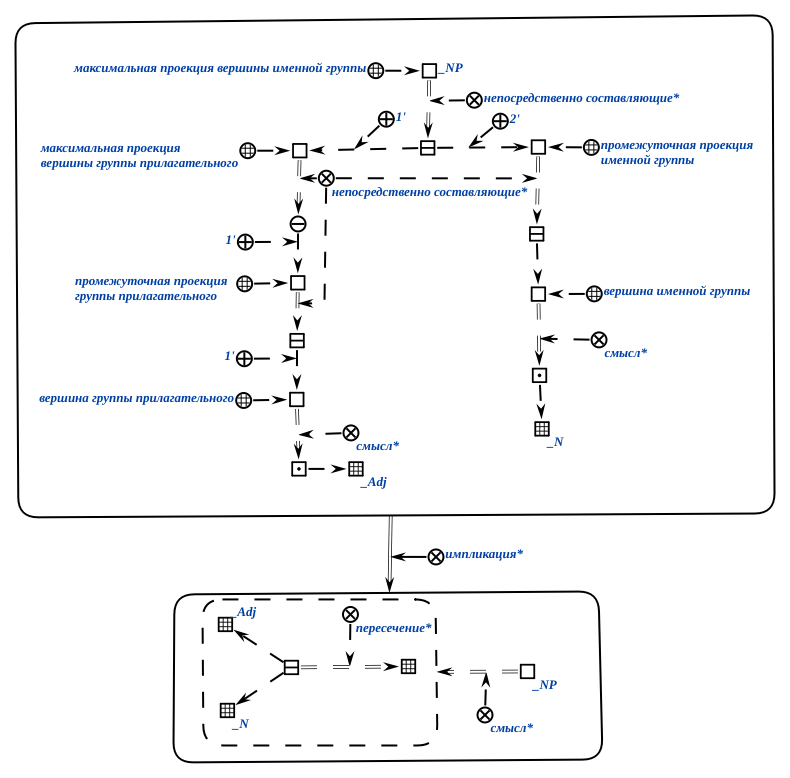
\includegraphics[width=0.8\textwidth]{images/part2/chapter_lang/d_sem_2.png}
    \caption{Правило интерпретации максимальной проекции вершины именной группы}
    \label{fig:d_sem_2}
\end{figure*}
%тут мы комбинируем смыслы прилагательного и существительного, которые входят в одну именную группу

На рисунке~\textit{\nameref{fig:d_sem_3}} приведено правило, по которому происходит интерпретация глагольной группы. Необходимость включения в посылку правила всей ветки глагольной группы объясняется ее необходимостью для определения типа глагола -- данное правило предназначено для интерпретации непереходных глаголов. Смыслом такой конструкции является класс действий.

\begin{figure*}[h]
    \centering
    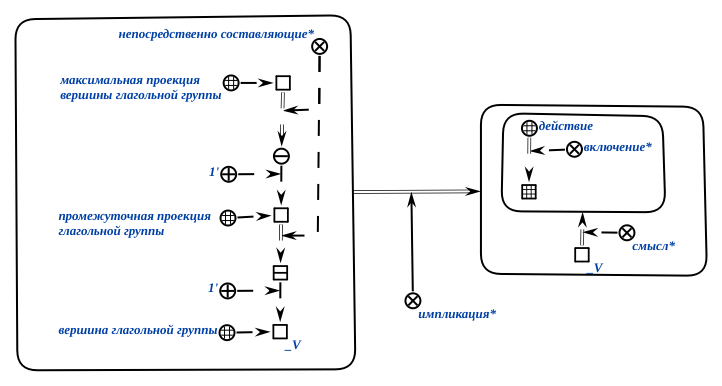
\includegraphics[width=0.8\textwidth]{images/part2/chapter_lang/d_sem_3.png}
    \caption{Правило интерпретации максимальной проекции вершины глагольной группы, содержащей непереходный глагол}
    \label{fig:d_sem_3}
\end{figure*}
%тут мы задаем интерпретацию всей глагольной группы (макс проекции) только для непереходных глаголов. написать, что смотрим по всей структуре группы целиком, потому что для того, чтобы отличить непереходный от переходного нам нужна вся ветка глагольной группы в дереве целиком

На рисунке~\textit{\nameref{d_sem_4}} приведено правило, по которому происходит интерпретация группы детерминанта с неопределенным артиклем. Смыслом такой конструкции является существование элемента класса, являющегося смыслом входящей в состав данной группы детерминанта именной группы.

\begin{figure*}[h]
    \centering
    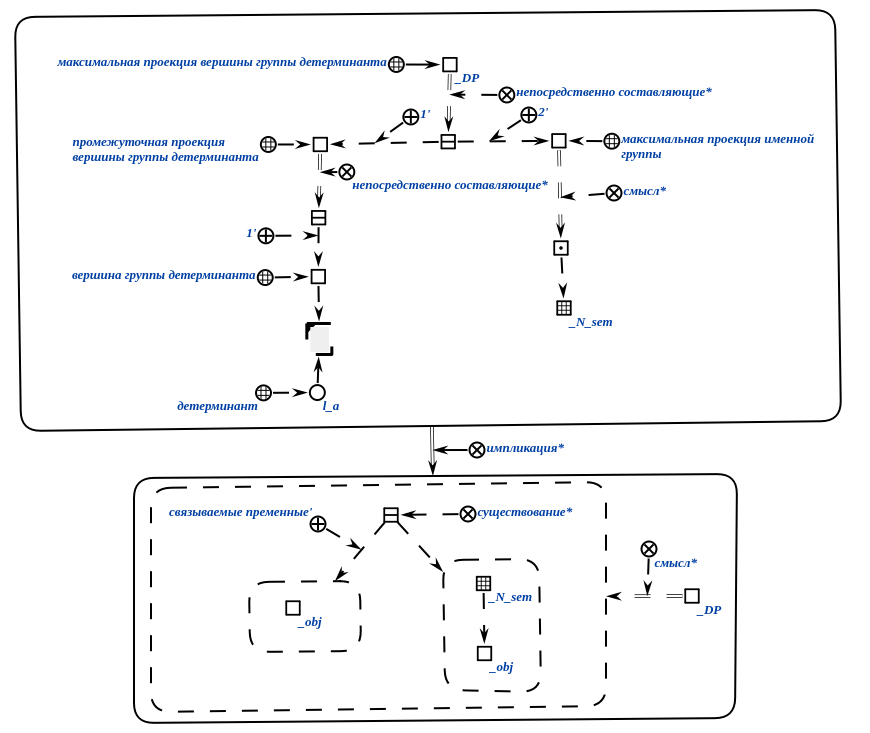
\includegraphics[width=0.8\textwidth]{images/part2/chapter_lang/d_sem_4.png}
    \caption{Правило интерпретации максимальной проекции вершины группы детерминанта}
    \label{d_sem_4}
\end{figure*}
%тут задается интерпретация сочетания именной группы с артиклем (в данном случае неопределенным)

На рисунке~\textit{\nameref{fig:d_sem_5}} приведено правило, по которому происходит интерпретация промежуточной проекции вершины временной группы, состоящей из вспомогательного глагола и полнозначного глагола. Вспомогательный глагол в данном случае задет класс действий по времени (является ли оно запланированным, выполняемым, уже выполненным и т.д.).

\begin{figure*}[h]
    \centering
    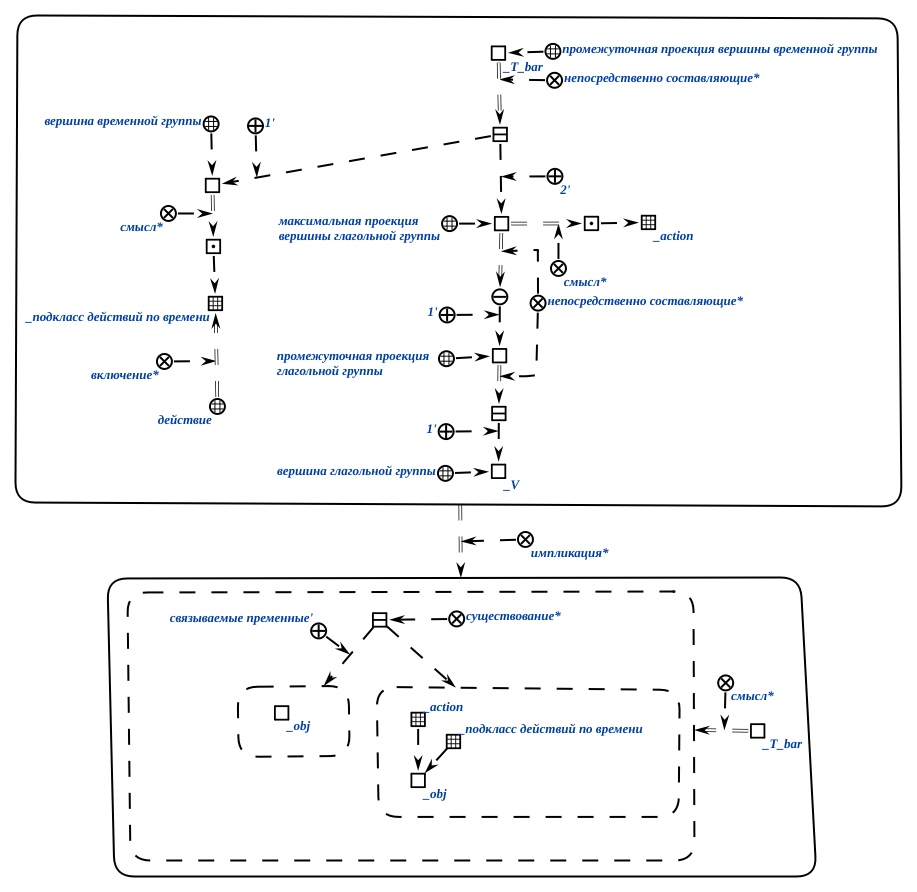
\includegraphics[width=0.8\textwidth]{images/part2/chapter_lang/d_sem_5.png}
    \caption{Правило интерпретации промежуточной проекции вершины временной группы}
    \label{fig:d_sem_5}
\end{figure*}
%тут задаем интерпретацию сочетания вспомогательного глагола и основного глагола. вспомогательный у нас соответствует классу действий по времени

На рисунке~\textit{\nameref{fig:d_sem_6}} приведено правило, по которому происходит интерпретация максимальной проекции вершины временной группы на основе полученного на предыдущем шаге смысла промежуточной проекции вершины временной группы и смысла максимальной проекции группы детерминанта.

\begin{figure*}[h]
    \centering
    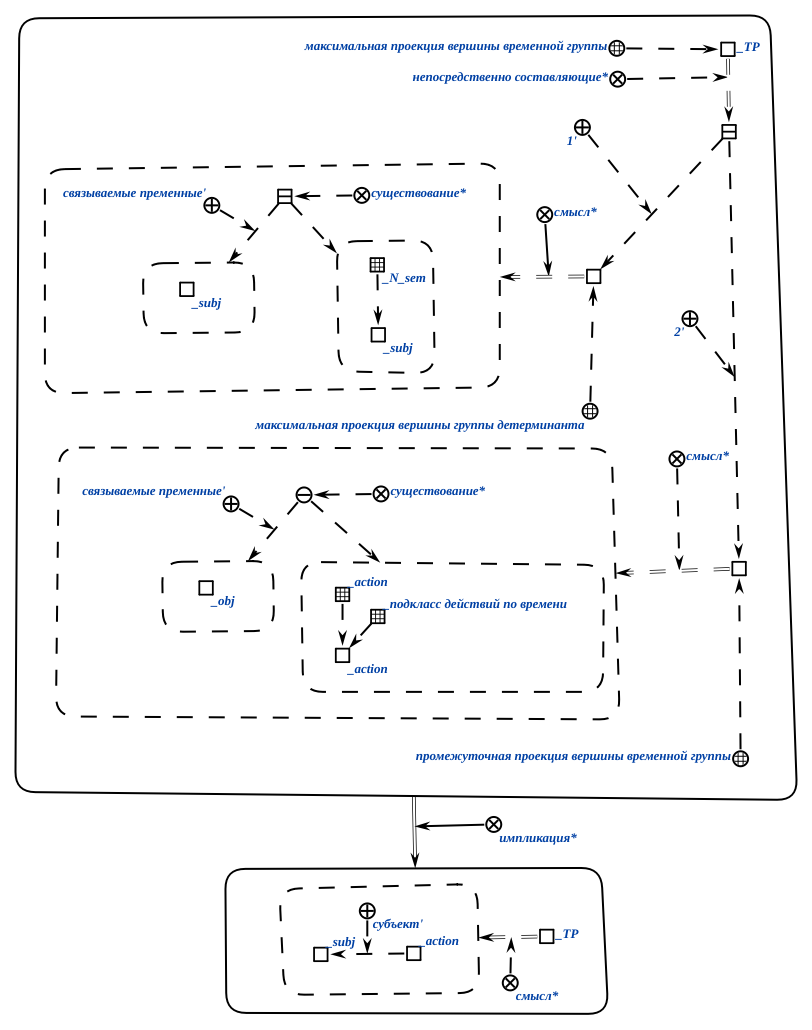
\includegraphics[width=0.8\textwidth]{images/part2/chapter_lang/d_sem_6.png}
    \caption{Правило интерпретации максимальной проекции вершины временной группы}
    \label{fig:d_sem_6}
\end{figure*}
%тут задаем интерпретацию для аргументной структуры непереходного глагола (сочетания подлежащего с непереходным глаголом)

На рисунке~\textit{\nameref{fig:d_sem_7}} приведено правило, по которому происходит интерпретация максимальной проекции вершины группы комплементатора на основе полученных на предыдущих шагах смыслов более частных конструкций. Данным правилом задается интерпретация предложения с переходным глаголом.

\begin{figure*}[h]
    \centering
    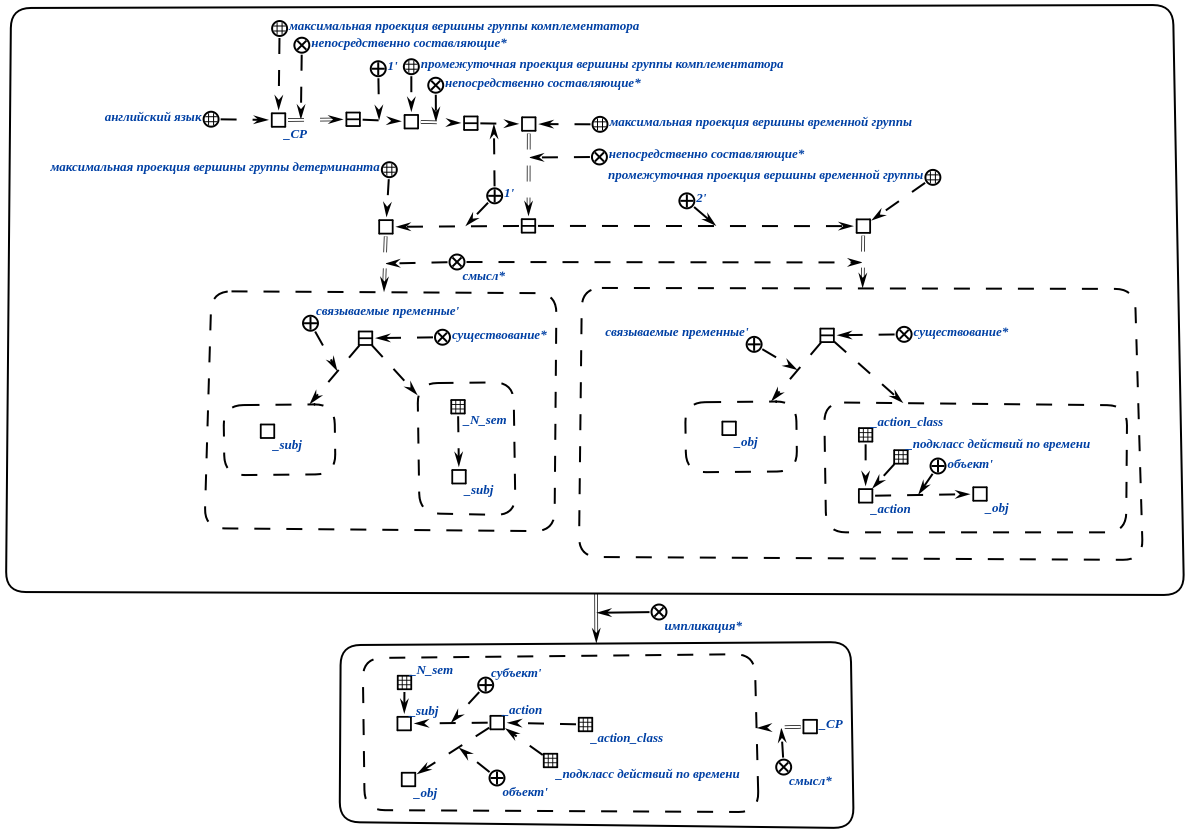
\includegraphics[width=0.8\textwidth]{images/part2/chapter_lang/d_sem_7.png}
    \caption{Правило интерпретации предложения с переходным глаголом}
    \label{fig:d_sem_7}
\end{figure*}
%тут задаем интерпретацию аргументной структуры переходного глагола (сочетания переходного глагола с его аргументами - подлажещим и дополнением)

%\input{author/references}